\documentclass[a4paper,pdftex]{book} 

\usepackage{fullpage}
%\usepackage{isolatin1} 
\usepackage{graphicx}
\usepackage{mathpazo}
\usepackage{listings}
\usepackage{longtable} %pour les preuves des programmes

\usepackage{lscape}    % pour le mode landscape
\usepackage{makeidx}
\usepackage{color}
\usepackage{amstext,url,latexsym,amsfonts,amssymb,amsmath,amsthm}
\usepackage{hyperref}


\newtheorem{example}{Example}
\newtheorem{theorem}{Theorem}
\newtheorem{algorithm}{Algorithm}
\newtheorem{propriete}{Property}

\DeclareMathOperator{\sinpi}{sinpi}
\DeclareMathOperator{\cospi}{cospi}
\DeclareMathOperator{\tanpi}{tanpi}
\DeclareMathOperator{\asinpi}{asinpi}
\DeclareMathOperator{\acospi}{acospi}
\DeclareMathOperator{\atanpi}{atanpi}
\DeclareMathOperator{\arccosh}{arccosh}


\newcommand{\pref}[1]{$<$\ref{#1}$>$}
\newcommand{\quick}{{quick}}
\newcommand{\accurate}{{accurate}}
\newcommand{\ulp}{\mbox{ulp}}
\newcommand{\crlibm}{\texttt{crlibm}}
\newcommand{\scslib}{\texttt{scslib}}

\renewcommand{\epsilon}{\varepsilon}

\newcommand{\round}{\circ}
\newcommand{\roundup}{\bigtriangleup}
\newcommand{\rounddown}{\bigtriangledown}
\newcommand{\intpart}[1]{\left\lceil #1 \right\rfloor}
\newcommand{\maxv}[1]{{\overline{#1}}}
\newcommand{\maxx}{\maxv{x}}
\newcommand{\maxeps}{\maxv{\epsilon}}
\newcommand{\maxdelta}{\maxv{\delta}}
\newcommand{\maxz}{{\overline{z}}}
\newcommand{\maxs}[1]{\overline{s}_{#1}}
\newcommand{\mins}[1]{\underline{s}_{#1}}
\newcommand{\maxp}{\overline{|P|}}
\newcommand{\minp}{\underline{|P|}}
\newcommand{\infnorm}[1]{||{#1}||^{\infty}}

\newcommand{\abserr}[1]{\delta_{\mathrm{#1}}}
\newcommand{\relerr}[1]{\epsilon_{\mathrm{#1}}}
\newcommand{\maxabserr}[1]{\maxv{\delta}_{\mathrm{#1}}}
\newcommand{\maxrelerr}[1]{\maxv{\epsilon}_{\mathrm{#1}}}

\newcommand{\N}{\ensuremath{\mathbb {N}}}
\newcommand{\Z}{\ensuremath{\mathbb {Z}}}
\newcommand{\F}{\ensuremath{\mathbb {F}}}
\newcommand{\R}{\ensuremath{\mathbb {R}}}
\newcommand{\hi}{\ensuremath{\mathit{h}}}
\newcommand{\mi}{\ensuremath{\mathit{m}}}
\newcommand{\lo}{\ensuremath{\mathit{l}}}
\newcommand{\E}{\ensuremath{\mathcal{E}}}
\newcommand{\Add}{{\bf Add12}}
\newcommand{\AddDD}{{\bf Add22}}
\newcommand{\AddDTT}{{\bf Add233}}
\newcommand{\AddDTTCond}{{\bf Add233Cond}}
\newcommand{\AdddTT}{{\bf Add133}}
\newcommand{\AddTT}{{\bf Add33}}
\newcommand{\MulDT}{{\bf Mul23}}
\newcommand{\Mul}{{\bf Mul12}}
\newcommand{\MulDD}{{\bf Mul22}}
\newcommand{\MulDTT}{{\bf Mul233}}
\newcommand{\MuldTT}{{\bf Mul133}}
\newcommand{\MuldDD}{{\bf Mul122}}
\newcommand{\MuldDT}{{\bf Mul123}}
\newcommand{\MulTT}{{\bf Mul33}}
\newcommand{\MulAddDdD}{{\bf MulAdd212}}
\newcommand{\MulAddDD}{{\bf MulAdd22}}
\newcommand{\SqrtD}{{\bf sqrt12}}
\newcommand{\SqrtT}{{\bf sqrt13}}
\newcommand{\Renormalize}{{\bf Renormalize3}}
\newcommand{\mAdd}{\ensuremath{\mathbf{Add12}}}
\newcommand{\mAddDD}{\ensuremath{\mathbf{Add22}}}
\newcommand{\mAddDTT}{\ensuremath{\mathbf{Add233}}}
\newcommand{\mAddDTTCond}{\ensuremath{\mathbf{Add233Cond}}}
\newcommand{\mAdddTT}{\ensuremath{\mathbf{Add133}}}
\newcommand{\mAddTT}{\ensuremath{\mathbf{Add33}}}
\newcommand{\mMul}{\ensuremath{\mathbf{Mul12}}}
\newcommand{\mMulDD}{\ensuremath{\mathbf{Mul22}}}
\newcommand{\mMulDT}{\ensuremath{\mathbf{Mul23}}}
\newcommand{\mMulDTT}{\ensuremath{\mathbf{Mul233}}}
\newcommand{\mMuldTT}{\ensuremath{\mathbf{Mul133}}}
\newcommand{\mMuldDD}{\ensuremath{\mathbf{Mul122}}}
\newcommand{\mMuldDT}{\ensuremath{\mathbf{Mul123}}}
\newcommand{\mMulAddDdD}{\ensuremath{\mathbf{MulAdd212}}}
\newcommand{\mMulAddDD}{\ensuremath{\mathbf{MulAdd22}}}
\newcommand{\mUlp}{\ensuremath{\mathrm{ulp}}}
\newcommand{\nan}{\ensuremath{\mathrm{NaN}}}
\newcommand{\sgn}{\ensuremath{\mathrm{sgn}}}
\renewcommand{\succ}{\ensuremath{\mathrm{succ}}}
\newcommand{\pred}{\ensuremath{\mathrm{pred}}}
\newcommand{\xor}{\ensuremath{\mbox{ }\mathrm{XOR}\mbox{ }}}
\newcommand{\Ord}{\ensuremath{\mathcal{O}}} 



%\newcommand{\deltapprox}{\delta_{\mathrm{approx}}}
%\newcommand{\deltaround}{\delta_{\mathrm{round}}}




% Environnement pour disposer de propri�t� ``� la leslie lamport''
\newcounter{propexp} % reset propexp � chaque chapitre
\newenvironment{prop}
{\begin{trivlist}\refstepcounter{propexp}\item[\hbox to 0pt{\spring {\bf $<$\arabic{propexp}$>$}}]}
{\ifvmode\smallskip\fi$\bullet$\end{trivlist}}

% D�finition de l'environnement proof
\def\spring{\hskip 0pt minus 1fil}
\def\@yproof[#1]{\@proof{ #1}}
\def\@proof#1{\begin{trivlist}\item[\hbox to 0pt{\spring $\diamond$}]
\emph{Proof#1. }}
\newenvironment{preuve}
{\@proof{}}{\hfill\null\hfill$\square$\end{trivlist}}



% Definition des options pour le packages listings
\lstset{numbers=left,
  numberstyle=\tiny,
  stepnumber=1,
  numbersep=5pt,
  lineskip=-1pt,
  extendedchars=true,
  basicstyle=\footnotesize,
  breaklines,
  showstringspaces=false,
  frame=single,
  language={[ANSI]C},
  firstnumber=last,
  escapeinside={(*@}{@*)}
}
 



\title{CR-LIBM\\A library of correctly rounded elementary functions in double-precision}
\author{\mbox{Catherine Daramy-Loirat}, \mbox{David Defour}, \mbox{Florent~de~Dinechin},\\ \mbox{Matthieu Gallet}, \mbox{Nicolas Gast},  \mbox{Christoph Quirin Lauter}, \mbox{Jean-Michel Muller}}

%% \abstract{
%%   CRLibm is a mathematical library with correct rounding in
%%   double-precision in the four IEEE-754 rounding modes. This report
%%   explains the code and proves the correct rounding property.
%% }

%% \RRIresume{%
%%   CRLibm est une biblioth�que math�matique offrant l'arrondi correct
%%   en double pr�cision selon les quatre modes d'arrondi. Ce rapport
%%   d�taille les algorithmes utilis�s et prouve fonction par fonction la
%%   propri�t� d'arrondi correct.
%% }%

%% \RRIkeywords{elementary functions, correct rounding, IEEE-754, double precision}

%% \RRImotscles{fonctions �l�mentaires, arrondi correct, IEEE-754, double pr�cision}

%% \RRItheme{2}

%% \RRIprojet{Ar�naire}

%% \RRIinria{\RRnote{%
%%     This  text  is  also  available   as  a  research  report  of  the
%%     Laboratoire    de     l'Informatique    du    Parall�lisme    {\tt
%%       http://www.ens-lyon.fr/LIP}.
%% }}%




\begin{document}
\maketitle


\section*{Important warning}

This report describes and proves version \input{../../VERSION} of the
\texttt{crlibm} library. It may therefore not correspond to the latest
version. An up-to-date version will always be distributed along with
the code.

\vfill
\section*{Many thanks to...}
\begin{itemize}
\item Vincent Lef\`evre, from \textsc{Inria}-Lorraine, without whom this
  project would't have started, and who has since then lended a helpful hand in
  more than 17 occasions;
\item The Ar\'enaire project at ENS-Lyon, especially Marc Daumas,
  Sylvie Boldo, Guillaume Melquiond, Nathalie Revol and Arnaud
  Tisserand;
\item Guillaume Melquiond for Gappa and its first-class hotline;
\item The MPFR developers, and especially the \textsc{Inria}
  \textsc{Spaces} project;
\item The Intel Nizhniy-Novgorod Lab, especially Andrey Naraikin,
  Sergei Maidanov and Evgeny Gvozdev;
\item The contributors of bits and pieces, Phil Defert and Eric
  McIntosh from CERN, Patrick Pelissier from \textsc{Inria};
\item All the people who have reported bugs, hoping that they continue
  until they have to stop: Evgeny Gvozdev from Intel with special
  thanks, Christoph Lauter from TUM\"unchen (before he joined the
  project), Eric McIntosh from CERN, Patrick Pelissier and Paul
  Zimmermann from \textsc{Inria} Lorraine;
\item William Kahan at UCBerkeley, Peter Markstein at HP, Neil Toda at
  Sun, Shane Story at Intel, and many others for interesting and
  sometimes heated discussions;
\item Serge Torres for LIPForge.
\end{itemize}

This work was partly funded by the \textsc{Inria}, the ENS-Lyon and
the Universit\'e de Perpignan.

\tableofcontents

\addtocounter{chapter}{-1}
\chapter{Getting started with crlibm}
\section{What is \crlibm?}

The \crlibm\ project aims at developing a portable, proven, correctly rounded,
and efficient mathematical library (\texttt{libm}) for double precision. 

\begin{description}
\item[correctly rounded] Current \texttt{libm} implementation do not
  always return the floating-point number that is closest to the exact
  mathematical result. As a consequence, different \texttt{libm}
  implementation will return different results for the same input,
  which prevents full portability of floating-point applications. In
  addition, few libraries support but the round-to-nearest mode of the
  IEEE754/IEC 60559 standard for floating-point arithmetic (hereafter
  usually referred to as the IEEE-754 standard). \crlibm\ provides the
  four rounding modes: To nearest, to $+\infty$, to $-\infty$ and to
  zero.

\item[portable] \crlibm\ is written in C and will be compiled by any
  compiler fulfilling basic requirements of the ISO/IEC 9899:1999
  (hereafter referred to as C99) standard.  This is the case of
  \texttt{gcc} version 3 and higher which is available on most
  computer systems. It also requires a floating-point implementation
  respecting the IEEE-754 standard, which is also available on
  most modern systems. \crlibm\ has been tested on a large range of
  systems.

\item[proven] Other libraries attempt to provide correctly-rounded
  result. For theoretical and practical reasons, this behaviour is
  difficult to prove, and in extreme cases termination is not even
  guaranteed. \crlibm\ intends to provide a comprehensive proof of the
  theoretical possibility of correct rounding, the algorithms used,
  and the implementation, assuming C99 and IEEE-754 compliance.

\item[efficient] performance and resource usage of \crlibm\ should be
  comparable to existing \texttt{libm} implementations, both in
  average and in the worst case. In contrast, other correctly-rounded
  libraries have worst case performance and memory consumption several
  order of magnitude larger than standard \texttt{libm}s.

\end{description}

The ultimate goal of the \crlibm\ project is to push towards the
standardization of correctly-rounded elementary functions.

\section{Compilation and installation}
See the \texttt{INSTALL} file in the main directory. This library is
developed using the GNU autotools, and can therefore be compiled on
most Unix-like systems by \texttt{./configure; make}. 


The command \texttt{make check} will launch the selftest.
For more advanced testing you will need to have MPFR installed (see
\url{www.mpfr.org}) and to pass the \texttt{--enable-mpfr} flag to
\texttt{configure}. For other flags, see \texttt{./configure --help} .

\section{Using \texttt{crlibm} functions in your program}

Currently \texttt{crlibm} functions have different names from the
standard \texttt{math.h} functions. For example, for the sine function
(\texttt{double sin(double)} in the standard \texttt{math.h}), you
have four different functions in \texttt{crlibm} for the four
different rounding modes. These functions are named \texttt{sin\_rn},
\texttt{sin\_ru}, \texttt{sin\_rd} and \texttt{sin\_rz} for round to the
nearest, round up, round down and round to zero respectively. These
functions are declared in the C header file \texttt{crlibm.h}.

The \texttt{crlibm} library relies on double-precision IEEE-754
compliant floating-point operations.  For some processors and some
operating systems (most notably IA32 and IA64 processors under
GNU/Linux), the default precision is set to double-extended.  On such
systems you will need to call the \texttt{crlibm\_init()} function
before using any \texttt{crlibm} function to ensure such compliance.
This has the effect of setting the processor flags to IEEE-754
double-precision with rounding to the nearest mode.  This function
returns the previous processor status, so that previous mode can be
restored using the function \texttt{crlibm\_exit()}. Note that you
probably only need one call to \texttt{crlibm\_init()} at the beginning
of your program, not one call before each call to a mathematical
function.

Here's an example function named \texttt{compare.c} using the cosine
function from \texttt{crlibm} library.

\begin{lstlisting}[label={chap0:lst:prog_example},caption={compare.c},firstnumber=1]
#include<stdio.h>
#include<math.h>
#include<crlibm.h>

int main(void){
  double x, res_libm, res_crlibm;

  crlibm_init(); /* no need here to save the old processor state returned by crlibm_init() */ 
  printf("Enter a floating point number: ");
  scanf("%lf", &x);
  res_libm = cos(x);
  res_crlibm = cos_rn(x);
  printf("\n x=%.25e \n", x);
  printf("\n cos(x) with the system : %.25e \n", res_libm);
  printf("\n cos(x) with crlibm     : %.25e \n", res_crlibm);
  return 0;
}
\end{lstlisting}

This example will be compiled with \texttt{gcc compare.c -lm -lcrlibm -o compare}


\section{Currently available functions}

The currently available functions are summarized in the following
table, where $x$ is of type $double$ and every function returns a
double-precision number. For trigonometric functions the angles are
expressed in radian.
\begin{center}
\begin{tabular}{|c|c|c|c|c|}    \hline
 & \multicolumn{4}{c|}{crlibm} \\ \cline{2-5}
 \raisebox{5pt}{C99} & to nearest & to $+ \infty$ & to $- \infty$ & to zero \\ \hline
    cos(x) & cos\_rn(x) & cos\_ru(x) & cos\_rd(x) & cos\_rz(x) \\ \hline
    sin(x) & sin\_rn(x) & sin\_ru(x) & sin\_rd(x) & sin\_rz(x) \\ \hline
    tan(x) & tan\_rn(x) & tan\_ru(x) & tan\_rd(x) & tan\_rz(x) \\ \hline
    cosh(x) & cosh\_rn(x) & cosh\_ru(x) & cosh\_rd(x) & cosh\_rz(x) \\ \hline
    sinh(x) & sinh\_rn(x) & sinh\_ru(x) & sinh\_rd(x) & sinh\_rz(x) \\ \hline
    atan(x) & atan\_rn(x) & atan\_ru(x) & atan\_rd(x) & atan\_rz(x) \\ \hline
    exp(x) & exp\_rn(x) & exp\_ru(x) & exp\_rd(x) & exp\_rz(x) \\ \hline
    log(x) & log\_rn(x) & log\_ru(x) & log\_rd(x) & log\_rz(x) \\ \hline
    log2(x) & log2\_rn(x) & log2\_ru(x) & log2\_rd(x) & log2\_rz(x) \\ \hline
    log10(x) & log10\_rn(x) & log10\_ru(x) & log10\_rd(x) & log10\_rz(x) \\ \hline
\end{tabular}
\end{center}



\section{Writing portable floating-point programs}

Here are some rules to help you design programs which have to
produce exactly the same results on different architectures and
different operating systems.
\begin{itemize}
\item Try to use the same compiler on all the systems.
\item Demand C99 compliance (pass the \texttt{-C99},
  \texttt{-std=c99}, or similar flag to the compiler). For Fortran,
  demand F90 compliance.
\item Call \texttt{crlibm\_init()} before you begin floating-point
  computation. This ensures that the computations will all be done in
  IEEE-754 double-precision with round to nearest mode, which is the
  largest precision well supported by most systems. On IA32
  processors, problems may still occur for extremely large or
  extremely small values.
\item Do not hesitate to rely heavily on parentheses (the compiler
  should respect them according to the standards, although of course some
  won't). Many times, wondering where the parentheses should go in an
  expression like \texttt{a+b+c+d} will even help you improve the
  accuracy of your code.
\item Use \texttt{crlibm} functions in place of \texttt{math.h} functions.
\end{itemize}



%%% Local Variables: 
%%% mode: latex
%%% TeX-master: "crlibm"
%%% End: 



\chapter{Introduction: Goals and methods \label{chap:intro}}



\section{Correct rounding and elementary functions}
\label{sect:intro}

The need for accurate elementary functions is important in many
critical programs.  Methods for computing these functions include
table-based methods\cite{Far81,Tan91}, polynomial approximations and
mixed methods\cite{DauMor2k}. See the books by Muller\cite{Muller97} or
Markstein\cite{Markstein2000} for recent surveys on the subject.

The IEEE-754 standard for floating-point arithmetic\cite{IEEE754}
defines the usual floating-point formats (single and double
precision). It also specifies the behavior of the four basic operators
($+,-,\times,\div$) and the square root in four rounding modes (to the
nearest, towards $+\infty$, towards $-\infty$ and towards $0$). Its
adoption and widespread use have increased the numerical quality of,
and confidence in floating-point code. In particular, it has improved
\emph{portability} of such code and allowed construction of
\emph{proofs} on its numerical behavior. Directed rounding modes
(towards $+\infty$, $-\infty$ and $0$) also enabled efficient
\emph{interval arithmetic}\cite{Moore66,KKLRW93}.

However, the IEEE-754 standard specifies nothing about elementary
functions, which limits these advances to code excluding such
functions.  Currently, several options exist: on one hand, one can use
today's mathematical libraries that are efficient but without any
warranty on the correctness of the results. When strict guarantees are
needed, some multiple-precision packages like MPFR \cite{MPFRweb}
offer correct rounding in all rounding modes, but are several orders
of magnitude slower than the usual mathematical libraries for the same
precision. The recently released IBM Ultimate Math
Library\cite{IBMlibultimweb} claims to offer correct rounding to the nearest,
and this library is both portable and fast, if bulky. However, for
reasons detailed below, this claim is not proven. Besides, this
library still lacks directed rounding modes needed for interval
arithmetic, and has other drawbacks that we analyze in the sequel.


The  goal of the \crlibm\ project is to build on a combination of several
recent advances to design a correctly rounded mathematical
library which is fast enough to replace the existing libraries, at a
minor cost in terms of performance and resources.




%%%%%%%%%%%%%%%%%%%%%%%%%%%%%%%%%%%%%%%%%%%%%%%%%%%%%%%%%%%%%
\section{A methodology for efficient correctly-rounded functions}
\label{section:methodology}


\subsection{The Table Maker's Dilemma}

With a few exceptions, the image $y$ of a floating-point number $x$ by
a transcendental function $f$ is a transcendental number, and can
therefore not be represented exactly in standard numeration systems.
The only hope is to compute the floating-point number that is closest
to (resp.  immediately above or immediately below) the mathematical
value, which we call the result \emph{correctly rounded} to the
nearest (resp.  towards $+\infty$ or towards $-\infty$).

It is only possible to compute an approximation $\hat{y}$ to the real
number $y$ with precision $\epsilon$. This ensures that the real value
$y$ belongs to the interval $[\hat{y}-\epsilon , \hat{y}+\epsilon]$.
Sometimes however, this information is not enough to decide correct
rounding. For example, if $[\hat{y}-\epsilon , \hat{y}+\epsilon]$
contains the middle of two consecutive floating-point numbers, it is
impossible to decide which of these two numbers is the correctly
rounded to the nearest of $y$. This is known as the Table Maker's
Dilemma (TMD).

\subsection{The onion peeling strategy}

A method described by Ziv \cite{Ziv91} is to increase the precision
$\epsilon$ of the approximation until the correctly rounded value can
be decided.  Given a function $f$ and an argument $x$, the value of
$f(x)$ is first evaluated using a quick approximation of precision
$\epsilon_1$.  Knowing $\epsilon_1$, it is possible to decide if
rounding is possible, or if more precision is required, in which case
the computation is restarted using a slower approximation of precision
$\epsilon_2$ greater than $\epsilon_1$, and so on. This approach makes
sense even in terms of average performance, as the slower steps are
rarely taken.

However there was until recently no practical bound on the termination
time of such an algorithm. This iteration has been proven to
terminate, but the actual maximal precision required in the worst case
is unknown.  This might prevent using this method in critical
application.




\section{The Correctly Rounded Mathematical Library}
\label{section:crlibm}

We have designed our own library called \emph{crlibm} (correctly
rounded mathematical library). It is based on the work of
Lef\`evre\cite{LMT98,Lef2000} who computed the worst-case $\epsilon$
required for correctly rounding several functions in double-precision
over selected intervals in the four IEEE-754 rounding modes. For
example, he proved that 157 bits are enough to ensure correct rounding
of the exponential function on all of its domain for the four IEEE-754
rounding modes.

\subsection{Two steps are enough}
Thanks to such results, we are able to guarantee correct rounding in
two iterations only, which we may then optimize separately. The first
of these iterations is relatively fast and provides between 60 and 80
bits of accuracy (depending on the function), which is sufficient in
most cases. It will be referred throughout this document as the \quick\ 
phase of the algorithm. The second phase, referred to as the
\accurate\ phase, is dedicated to challenging cases. It is slower but
has a reasonably bounded execution time, tightly targeted at
Lef\`evre's worst cases.

Having a proven worst-case execution time lifts the last obstacle to a
generalization of correctly rounded transcendentals. Besides, having
only two steps allows us to publish, along with each function, a proof
of its correctly rounding behavior.


\subsection{Portable IEEE-754 FP for fast first step}
The computation of a tight bound on the approximation error of the
first step ($\epsilon_1$) is crucial for the efficiency of the onion
peeling strategy: overestimating $\epsilon_1$ means going more often
than needed through the second step. As we want the proof to be
portable as well as the code, our first steps are written in strict
IEEE-754 arithmetic. On some systems, this means preventing the
compiler/processor combination to use advanced floating-point features
such as fused multiply-and-add or extended double precision. It also
means that the performance of our portable library will be lower than
optimized libraries using these features.

To ease these proofs, our first steps make wide use of classical, well
proven techniques. In particular, when a result is needed in a
precision higher than double precision (as is the case of $\hat{y_1}$,
the result of the first step), it is represented as as the sum of two
floating-point numbers. There are well-known algorithms for computing
on such sums (for instance Sterbenz' lemma, the Fast2Sum algorithm,
the Dekker algorithm\cite{Knu73}) with mechanically checked proofs.

A sequence of simple tests on $\hat{y_1}$ allows to decide whether to
go for the second step. The sequence corresponding to each rounding
mode is shared by most functions and has also been carefully proven.


\subsection{Software Carry-Save for an accurate second step}
For the second step, we designed an ad-hoc multiple-precision library
called Software Carry-Save library \emph{(scslib)} which is lighter
and faster than other available libraries for this specific
application \cite{DefDin2002,DinDef2003}. This choice is motivated by
considerations of code size and performance, but also by the need to
be independent of other libraries: Again, we need a library on which
we may rely at the proof level. This library is independent from the
mathematical library and distributed separately \cite{SCSweb}.


\subsection{Current state of \emph{crlibm}}

The library \texttt{crlibm} \emph{(correctly rounded mathematical
  library)} currently offers accurate parts for the exponential,
logarithm in radix $2$, $10$ and $e$, sine, cosine, tangent,
arctangent, plus trigonometric argument reduction. The first quick
part and its proof have only been written for the exponential thus
far. The difficulty is to prove both the algorithm and the C program.
The proof relies heavily on several shared lemmas, assuming the good
behavior of the system composed of the compiler and the processor.
Another difficulty is that performance is important. Therefore many
parts of this proof could be done only by hand.


\subsection{Organization of the source code of the library}

For each function, the file containing the source code for the
accurate phase is named after the function itself (for instance
\texttt{exp.c}, \texttt{log.c}), and the quick phase, when available,
is named with the \texttt{\_fast} suffix (for instance
\texttt{exp\_fast.c}). The names of auxiliary files \texttt{.c} or
\texttt{.h} files relative to a function are also prefixed with the
name of the function.

The accurate phase relies on \texttt{scslib}, the \emph{software
  carry-save} multiple-precision library written for this purpose.
This library is contained in a subdirectory called \texttt{scs\_lib}.

The common C routines that are detailed in Part~\ref{sec:common} of
this document are defined in \texttt{crlibm\_private.c} and
\texttt{crlibm\_private.h}.

Many of the constants used in the C code have been computed thanks to
Maple procedures which are contained in the \texttt{maple}
subdirectory. Some of these procedures are explained in
Part~\ref{sec:common}. For some functions, a Maple procedure mimicking
the C code, and used for debugging or optimization purpose, is also
available.




\section{An overview of other  available mathematical libraries\label{section:lib-overview}}

Many high-quality mathematical libraries are freely available and have
been a source of inspiration for this work.

Most mathematical libraries do not offer correct rounding. They can be classified as 
\begin{itemize}
\item portable libraries  assuming IEEE-754
  arithmetic, like \emph{fdlibm}, written by Sun\cite{FDLIBMweb} and \emph{libultim}
  written by IBM\cite{IBMlibultimweb};
\item  Processor-specific libraries, by
  Intel\cite{HarKubStoTan99,IntelOpenSource} and
  HP\cite{Markstein2000,Markstein2001} among other.
\end{itemize}

Operating systems often include several mathematical libraries, some of which are derivatives of one
of the previous.

Two libraries offering correct correct rounding are specially relevant to this work:
\begin{itemize}
\item The\emph{libultim} library also called MathLib, is developed at
  IBM by Ziv and others \cite{IBMlibultimweb}. It provides correct rounding,
  under the assumption that 800 bits are enough in all case. This
  approach suffers two weaknesses. The first is the absence of proof
  that 800 bits are enough: all there is is a very high probability.
  The second is that, as we will see in the sequel, for challenging
  cases, 800 bits are much of an overkill, which can increase the
  execution time up to 20,000 times a normal execution. This will
  prevent such a library from being used in real-time applications.
  Besides, to prevent this worst case from degrading average
  performance, there is usually some intermediate levels of precision
  in MathLib's elementary functions, which makes the code larger, more
  complex, and more difficult to prove.
  
  In addition this library provides correct rounding only to nearest.
  This is the most used rounding mode, but it might not be the most
  important as far as correct rounding is concerned: correct rounding
  provides a precision improvement over current mathematical libraries
  of only a fraction of a {unit in the last place} \emph{(ulp)}.
  Conversely, the three other rounding modes are needed to guarantee
  intervals in interval arithmetic.  Without correct rounding in these
  directed rounding modes, interval arithmetic looses up to one
  \emph{ulp} of precision in each computation.
  
\item \emph{MPFR} is a multiprecision package safer than
  \emph{libultilm} as it uses arbitrary multiprecision. It provides
  most of elementary functions for the four rounding modes defined by
  the IEEE-754 standard. However this library is not optimized for
  double precision arithmetic. In addition, as its exponent range is
  much wider than that of IEEE-754, the subtleties of denormal numbers
  are difficult to handle properly using such a multiprecision
  package.
\end{itemize}

The \texttt{crlibm} code includes programs to test the \texttt{crlibm}
functions against MPFR and \texttt{libultim}. They are located in the
\texttt{tests} directory.



\chapter{Common notations, theorems and procedures \label{chap:common}}
% Common notations, theorems and procedures

\section{Notations\label{section:notations}}


The following notations will be used throughout this document:
\begin{itemize}

\item  $+$, $-$ and  $\times$ denote the usual
mathematical operations.

\item $\oplus$, $\ominus$ and $\otimes$ denote the
corresponding floating-point operations in IEEE-754 double precision,
in the IEEE-754 \emph{round to nearest} mode.

\item $\round(x)$, $\roundup(x)$ and $\rounddown(x)$ denote the value
  of $x$ rounded to the nearest, resp. rounded up and down.
  
\item $\epsilon$ (usually with some index) denotes a relative error,
  $\delta$ denotes an absolute error. Upper bounds on the absolute value of these errors
  will be denoted $\maxeps$ and $\maxdelta$.

\item $\maxeps_{-k}$ -- with a negative index -- represents an error $e$ such that $|e| \leq 2^{-k}$.
  
\item For a floating-point number $x$, the value of the least
  significant bit of its mantissa is classically denoted $\ulp(x)$.

\end{itemize}




\section{Common C procedures for double-precision numbers\label{section:commonCdouble}}

\subsection{Sterbenz Lemma \label{sec:sterbenz}}

\begin{theorem}[Sterbenz Lemma~\cite{Ste74,Gol91}]
\label{sterbenz}
If $x$ and $y$ are floating-point numbers, and if ${y}/{2} \leq x \leq
2y$ then $x\ominus y$ is computed exactly, without any rounding error.
\end{theorem}


\subsection{Double-precision numbers in memory\label{section:memory}}

A double precision floating-point number uses $64$ bits. The unit of
memory in most current architectures is a 32-bit word. The order in
which the two $32$ bits words of a double are stored in memory depends
on the architecture. An architecture is said \emph{Little Endian} if
the lower part of the number is stored in memory at the smallest
address; It is the case of the x86 processors. Conversely, an
architecture with the high part of the number stored in memory at the
smallest address is said \emph{Big Endian}; It is the case of the
PowerPC processors.

In \crlibm, we extract the higher and lower parts of a double by using
an union in memory: the type \texttt{db\_number}. The following code
extracts the upper and lower part from a double precision number $x$.

\begin{lstlisting}[label={chap0:lst:endian},
  caption={Extract upper and lower part of a double precision number $x$},firstnumber=1]
  /* HI and LO are defined automatically by autoconf/automake.  */

db_number xx;
int x_hi, x_lo;
xx.d = x;
x_hi = xx.i[HI]
x_lo = xx.i[LO]
\end{lstlisting}




\subsection{Conversion from floating-point to integer \label{sec:double2int}}

\begin{theorem}[Conversion floating-point to integer]
  The following algorithm, taken from \cite{AMDoptim2001}, converts a
  double-precision floating-point number $d$ into a 32-bit
  integer $i$ with rounding to nearest mode.

  It works for all the doubles whose nearest integer fits on a 32-bit machine signed integer.

\begin{lstlisting}[label={chap0:lst:conversion2},caption={Conversion from FP to int},firstnumber=1]
#define DOUBLE2INT(i, d)   \
  {double t=(d+6755399441055744.0); i=LO(t);}
\end{lstlisting}
\end{theorem}

This algorithm adds the constant $2^{52}+2^{51}$ to the floating-point
number to put the integer part of $x$, in the lower part of the
floating-point number.  We use $2^{52}+2^{51}$ and not $2^{52}$,
because the value $2^{51}$ is used to contain possible carry
propagations with negative numbers.


\subsection{Conversion from floating-point to 64-bit integer \label{sec:double2longint}}

\begin{theorem}[Conversion floating-point to a long long integer]
  The following algorithm, is derived from the previous.

  It works for any double whose nearest integer is smaller than $2^{51} -1$.

\begin{lstlisting}[label={chap0:lst:conversion3},caption={Conversion from FP to long long int},firstnumber=1]
#define DOUBLE2LONGINT(i, d)                                      \
  {                                                               \
    db_number t;                                                  \
    t.d = (d+6755399441055744.0);                                 \
    if (d >= 0) /* sign extend */                                 \
      i = t.l & 0x0007FFFFFFFFFFFFLL;                             \
    else                                                          \
      i = (t.l & 0x0007FFFFFFFFFFFFLL) |  (0xFFF8000000000000LL); \
  }
\end{lstlisting}

\end{theorem}




\subsection{Methods to raise IEEE-754 flags}

The IEEE standard imposes, in certain cases, to raise flags and/or
exceptions for the $4$ operators ($+$, $\times$, $\div$, $\sqrt{~}$).
Therefore, it is legitimate to require the same for elementary
functions.

In ISO C99, the following instructions raise exceptions and
flags:

\begin{itemize}
\item {\bf underflow} : the multiplication $\pm smallest \times smallest$ where $smallest$ correspond to the smallest subnormal number,
\item {\bf overflow} : the multiplication  $\pm largest \times largest$ where $largest$ correspond to the largest normalized number,
\item {\bf division by zero} : the division $\pm 1.0/0.0$,
\item {\bf inexact} : the addition $(x + smallest) - smallest$ where $x$ is the result and  $smallest$ the smallest subnormal number,
\item {\bf invalid} : the division $\pm 0.0/0.0$.
\end{itemize}








\section{Common C procedures for double-double arithmetic\label{section:commonCdoubledouble}}
Hardware operators are usualy limited to double precision. To perform
operations with more precision, then software solutions need to be
used. One among them is to represent a floating point number as the
sum of two non-overlapping floating-point numbers (or
\emph{double-double} numbers). 

The algorithms are given as plain C functions, but it may be
preferable, for performance issue, to implement them as macros, as in
\texttt{libultim}.  The code offers both versions,
selected by the \texttt{DEKKER\_AS\_FUNCTIONS} constant which is set
by default to 1 (functions).

A more recent proof is available in \cite{Lauter2005LIP:tripledouble}.

\subsection{Exact sum algorithm {Add12}}

This algorithm is also known as the Fast2Sum algorithm in the
litterature.
\begin{theorem}[Exact sum~\cite{Knu73, Boldo2001}]
  Let $a$ and $b$ be floating-point numbers, then the following method
  computes two floating-point numbers $s$ and $r$, such that $s+r =
  a+b$ exactly, and $s$ is the floating-point number which is closest
  to $a+b$.

\begin{lstlisting}[label={lst:Add12Cond},caption={Add12Cond},firstnumber=1]
void Add12Cond(double *s, double *r, a, b) 
{
  double z;
  s = a + b;            
  if (ABS(a) > ABS(b)){  
    z = s - a;           
    r = b - z;           
  }else {                 
    z = s - b;           
    r = a - z;           
  } 
}                         
\end{lstlisting}
Here ABS is a macro that returns the absolute value of a
floating-point number. This algorithm requires $4$ floating-point additions and $2$ floating
point tests (some of which are hidden in the ABS macro). 

Note that if it is more efficient on a given architecture, the test can be replaced
with a test on the exponents of $a$ and $b$.

\end{theorem}


If we are able to prove that  the exponent of $a$ is always greater than that
of $b$, then the previous algorithm to perform an exact addition of 2
floating-point numbers becomes :
\begin{lstlisting}[label={lst:Add12},caption={Add12},firstnumber=1]
void Add12(double *s, double *r, a, b) 
{
  double z;
  s = a + b;            
  z = s - a;  
  r = b - z; 
}            
\end{lstlisting}
The cost of this algorithm is $3$ floating-point additions.






\subsection{Exact product algorithm {Mul12}}

This algorithm is sometimes also known as the Dekker algorithm
\cite{Dek71}. It was proven by Dekker but the proof predates the
IEEE-754 standard and is difficult to read. An easier proof is
available in \cite{Gol91} (see Th. 14).

\begin{theorem}[Restricted exact product]
  Let $a$ and $b$ be two double-precision floating-point numbers, with
  53 bits of mantissa. Let $c=2^{\lceil\frac{ 53}{2} \rceil}+1$.
  Assuming that $a<2^{970}$ and $b<2^{970}$, the following procedure
  computes the two floating-point numbers $rh$ and $rl$ such that $rh
  + rl = a + b$ with $rh = a \otimes b$:
\begin{lstlisting}[label={lst:Mul12},caption={Mul12},firstnumber=1]
void  Mul12(double *rh, double *rl, double u, double v){
  const double c = 134217729.;   /*  1+2^27 */ 
  double up, u1, u2, vp, v1, v2;

  up = u*c;        vp = v*c;
  u1 = (u-up)+up;  v1 = (v-vp)+vp;
  u2 = u-u1;       v2 = v-v1;
  
  *rh = u*v;
  *rl = (((u1*v1-*rh)+(u1*v2))+(u2*v1))+(u2*v2);
}
\end{lstlisting}
\end{theorem}

The cost of this algorithm is $10$ floating-point
additions and $7$ floating-point multiplications.



The condition $a<2^{970}$ and $b<2^{970}$ prevents overflows when
multiplying by $c$. If it cannot be proved statically, then we have to
first test $a$ and $b$, and prescale them so that the condition is
true.


\begin{theorem}[Exact product]
  Let $a$ and $b$ be two double-precision floating-point numbers, with
  53 bits of mantissa. Let $c=2^{\lceil\frac{ 53 }{2}\rceil}+1$.
  The following procedure
  computes the two floating-point numbers $rh$ and $rl$ such that $rh
  + rl = a + b$ with $rh = a \otimes b$:

\begin{lstlisting}[label={lst:Mul12Cond},caption={Mul12Cond},firstnumber=1]
void Mul12Cond(double *rh, double *rl, double a, double b){
  const double two_970 = 0.997920154767359905828186356518419283e292;
  const double two_em53 = 0.11102230246251565404236316680908203125e-15;
  const double two_e53  = 9007199254740992.;
  double u, v;

  if (a>two_970)  u = a*two_em53; 
  else            u = a;
  if (b>two_970)  v = b*two_em53; 
  else            v = b;

  Mul12(rh, rl, u, v);

  if (a>two_970) {*rh *= two_e53; *rl *= two_e53;} 
  if (b>two_970) {*rh *= two_e53; *rl *= two_e53;} 
}\end{lstlisting}
\end{theorem}

The cost in the worst case is then $4$ tests over integers,
$10$ floating-point additions and $13$ floating-point multiplications.


Finally, note that a fused multiply-and-add provides the Mul12 and
Mul12Cond in only two instructions \cite{CorneaHarrisonTang2002}. Here
is the example code for the Itanium processor.

\begin{lstlisting}[label={lst:Mul12CondFMA},caption={Mul12 on the Itanium},firstnumber=1]
#define Mul12Cond(rh,rl,u,v)                          \
{                                                     \
  *rh = u*v;                                          \
  /* The following means: *rl = FMS(u*v-*rh) */       \
  __asm__ __volatile__("fms %0 = %1, %2, %3\n ;;\n"   \
                       : "=f"(*rl)                    \
                       : "f"(u), "f"(v), "f"(*rh)     \
                       );                             \
}
#define Mul12 Mul12Cond
\end{lstlisting}

The \crlibm\ distribution attempts to use the FMA for systems on which
it is availables (currently Itanium and PowerPC).




\subsection{Double-double addition {Add22}}
  
This algorithm, also due to Dekker \cite{Dek71}, computes the sum of
two double-double numbers as a double-double, with a relative error
smaller than $2^{-103}$ (there is a proof in \cite{Dek71}, a more recent one can be found in in \cite{Lauter2005LIP:tripledouble}).


\begin{lstlisting}[label={Add22Cond},caption={Add22Cond},firstnumber=1]
void Add22Cond(double *zh, double *zl, double xh, double xl, double yh, double yl)
{
double r,s;

r = xh+yh;
s = (ABS(xh) > ABS(yh))? (xh-r+yh+yl+xl) : (yh-r+xh+xl+yl);
*zh = r+s;
*zl = r - (*zh) + s;
}
\end{lstlisting}

Here ABS is a macro that returns the absolute value of a
floating-point number. Again, if this test can be resolved at
compile-time, we get the faster \texttt{Add22} procedure:

\begin{lstlisting}[label={Add22},caption={Add22},firstnumber=1]
void Add22(double *zh, double *zl, double xh, double xl, double yh, double yl)
{
double r,s;

r = xh+yh;
s = xh-r+yh+yl+xl;
*zh = r+s;
*zl = r - (*zh) + s;
}
\end{lstlisting}




\subsection{Double-double multiplication {Mul22}}
  
This algorithm, also due to Dekker \cite{Dek71}, computes the product of
two double-double numbers as a double-double, with a relative error
smaller than $2^{-102}$, under the condition $x_h<2^{970}$ and $y_h<2^{970}$  (there is a proof in \cite{Dek71}, a more recent one can be found in in \cite{Lauter2005LIP:tripledouble}). 

\begin{lstlisting}[label={Mul22},caption={Mul22},firstnumber=1]
void Mul22(double *zh, double *zl, double xh, double xl, double yh, double yl)
{
double mh, ml;

  const double c        = 134217729.;                /* 0x41A00000, 0x02000000 */ 
  double up, u1, u2, vp, v1, v2;

  up = xh*c;        vp = yh*c;
  u1 = (xh-up)+up;  v1 = (yh-vp)+vp;
  u2 = xh-u1;       v2 = yh-v1;
  
  mh = xh*yh;
  ml = (((u1*v1-mh)+(u1*v2))+(u2*v1))+(u2*v2);

  ml += xh*yl + xl*yh;
  *zh = mh+ml;
  *zl = mh - (*zh) + ml;
}  
\end{lstlisting}

Note that the bulk of this algorithm is a \texttt{Mul12(mh,ml,xh,yh)}.
Of course there is a conditional version of this procedure but we have not needed it so far.

%Our algorithms will sometimes need to multiply a double by a
%double-double. In this case we use \texttt{Mul22} with one of the
%arguments set to zero, which only performs one useless multiplication
%by zero and one useless addition: a specific procedure is not needed.


\subsection{The multiplication procedure \MuldDD}
\begin{algorithm}[\MuldDD] \label{muldDDref} ~ \\
{\bf In:} a double precision number $a$ and a double-double number $b_\hi + b_\lo$ \\
{\bf Out:} a double-double number $r_\hi + r_\lo$ \\
{\bf Preconditions on the arguments:}
\begin{eqnarray*}
\left \vert b_\lo \right \vert & \leq & 2^{-53} \cdot \left \vert b_\hi \right \vert 
\end{eqnarray*}
{\bf Algorithm:} \\
\begin{center}
\begin{minipage}[b]{60mm}
$\left( t_1, t_2 \right) \gets \mMul\left( a, b_\hi \right)$ \\
$t_3 \gets a \otimes b_\lo$ \\
$t_4 \gets t_2 \oplus t_3$ \\
$\left( r_\hi, r_\lo \right) \gets \mAdd\left( t_1, t_4 \right)$ \\
\end{minipage}
\end{center}
\end{algorithm}
\begin{theorem}[Relative error of algorithm \ref{muldDDref} \MuldDD] ~ \\
Let be $a$ and $b_\hi + b_\lo$ the values taken by 
the arguments of algorithm \ref{muldDDref} \MuldDD \\
So the following holds for the values returned $r_\hi$ and $r_\lo$:
$$r_\hi + r_\lo = 
\left( a \cdot \left( b_\hi + b_\lo \right)\right) \cdot 
\left(1 + \epsilon\right)$$
where $\epsilon$ is bounded as follows:
$$\left \vert \epsilon \right \vert \leq 2^{-102}$$
The values returned $r_\hi$ and $r_\lo$ will not overlap at all. 
\end{theorem}

\subsection{Double-double Horner step procedures\label{sec:double-double-horner}}

\subsubsection{The multiply-and-add operator \MulAddDdD}

\begin{algorithm}[\MulAddDdD] \label{MulAddDdDref} ~ \\
{\bf In:} a double-double number $c_\hi + c_\lo$, a double precision number $a$ and 
a double-double number $b_\hi + b_\lo$ \\
{\bf Out:} a double-double number $r_\hi + r_\lo$ \\
{\bf Preconditions on the arguments:}
\begin{eqnarray*}
\left \vert b_\lo \right \vert & \leq & 2^{-53} \cdot \left \vert b_\hi \right \vert \\
\left \vert c_\lo \right \vert & \leq & 2^{-53} \cdot \left \vert c_\hi \right \vert \\
\left \vert a \cdot \left( b_\hi + b_\lo \right) \right \vert & \leq & 2^{-2} \cdot \left \vert c_\hi + c_\lo \right \vert 
\end{eqnarray*}
{\bf Algorithm:} \\
\begin{center}
\begin{minipage}[b]{50mm}
$\left(t_1, t_2 \right) \gets \mMul\left( a , b_\hi \right)$ \\
$\left(t_3, t_4 \right) \gets \mAdd\left( c_\hi , t_1 \right)$ \\
$t_5 \gets b_\lo \otimes a$ \\
$t_6 \gets c_\lo \oplus t_2$ \\
$t_7 \gets t_5 \oplus t_6$ \\
$t_8 \gets t_7 \oplus t_4$ \\
$\left(r_\hi, r_\lo \right) \gets \mAdd\left( t_3 , t_8 \right)$ \\
\end{minipage}
\end{center}
\end{algorithm}
\begin{theorem}[Relative error of algorithm \ref{MulAddDdDref} \MulAddDdD\label{theoMulAddDdDref}] ~ \\
Let be $c_\hi + c_\lo$, $a$ and $b_\hi + b_\lo$ the 
arguments of algorithm \ref{MulAddDdDref} \MulAddDdD~ verifying the given 
preconditions.\\
So the following egality will hold for the returned values $r_\hi$ and $r_\lo$ 
$$r_\hi + r_\lo = \left( \left( c_\hi + c_\lo \right) + a \cdot \left( b_\hi + b_\lo \right) \right) \cdot 
\left( 1 + \epsilon \right)$$
where $\epsilon$ is bounded by:
$$\left \vert \epsilon \right \vert \leq 2^{-100}$$
The returned values $r_\hi$ and $r_\lo$ will not overlap at all.
\end{theorem}

\subsubsection{The multiply-and-add operator \MulAddDD}

\begin{algorithm}[\MulAddDD] \label{MulAddDDref} ~ \\
{\bf In:} three double-double numbers $c_\hi + c_\lo$, $a_\hi + a_\lo$ and 
$b_\hi + b_\lo$ \\
{\bf Out:} a double-double number $r_\hi + r_\lo$ \\
{\bf Preconditions on the arguments:}
\begin{eqnarray*}
\left \vert a_\lo \right \vert & \leq & 2^{-53} \cdot \left \vert a_\hi \right \vert \\
\left \vert b_\lo \right \vert & \leq & 2^{-53} \cdot \left \vert b_\hi \right \vert \\
\left \vert c_\lo \right \vert & \leq & 2^{-53} \cdot \left \vert c_\hi \right \vert \\
\left \vert \left( a_\hi + a_\lo \right) \cdot \left( b_\hi + b_\lo \right) \right \vert & 
\leq & 2^{-2} \cdot \left \vert c_\hi + c_\lo \right \vert 
\end{eqnarray*}
{\bf Algorithm:} \\
\begin{center}
\begin{minipage}[b]{50mm}
$\left(t_1, t_2 \right) \gets \mMul\left( a_\hi , b_\hi \right)$ \\
$\left(t_3, t_4 \right) \gets \mAdd\left( c_\hi , t_1 \right)$ \\
$t_5 \gets a_\hi \otimes b_\lo$ \\
$t_6 \gets a_\lo \otimes b_\hi$ \\
$t_7 \gets t_2 \oplus c_\lo$ \\
$t_8 \gets t_4 \oplus t_7$ \\
$t_9 \gets t_5 \oplus t_6$ \\
$t_{10} \gets t_8 \oplus t_9$ \\
$\left(r_\hi, r_\lo \right) \gets \mAdd\left( t_3 , t_{10} \right)$ \\
\end{minipage}
\end{center}
\end{algorithm}
\begin{theorem}[Relative error of algorithm \ref{MulAddDDref} \MulAddDD\label{theoMulAddDDref}] ~ \\
Let be $c_\hi + c_\lo$, $a_\hi + a_\lo$ and $b_\hi + b_\lo$ the 
arguments of algorithm \ref{MulAddDDref} \MulAddDD~ verifying the given 
preconditions.\\
So the following egality will hold for the returned values $r_\hi$ and $r_\lo$ 
$$r_\hi + r_\lo = \left( \left( c_\hi + c_\lo \right) + 
\left( a_\hi + a_\lo \right) \cdot \left( b_\hi + b_\lo \right) \right) \cdot 
\left( 1 + \epsilon \right)$$
where $\epsilon$ is bounded by:
$$\left \vert \epsilon \right \vert \leq 2^{-100}$$
The returned values $r_\hi$ and $r_\lo$ will not overlap at all.
\end{theorem}

\subsection{Multiplication of a double-double by an integer}


Use Cody and Waite algorithm. See for instance the $\log$ and the
trigonometric argument reduction (chapter \ref{chap:log}, p.
\pageref{chap:log}).


\section{Common C procedures for triple-double arithmetic\label{section:commonCtripledouble}}

These procedures are used to reach accuracies of about 150 bits. They
are detailed and proven in \cite{Lauter2005LIP:tripledouble}.
 

\begin{algorithm}[Renormalization] \label{renormalg}~\\
{\bf In: $a_\hi, a_\mi, a_\lo \in \F$} verifying the following preconditions:\\
{\bf Preconditions: }
\begin{itemize}
\item None of the numbers $a_\hi, a_\mi, a_\lo$ is subnormal
\item $a_\hi$ et $a_\mi$ do not overlap in more than $51$ bits
\item $a_\mi$ et $a_\lo$ do not overlap in more than $51$ bits
\end{itemize}
which means formally:
\begin{eqnarray*}
\left \vert a_\mi \right \vert & \leq & 2^{-2} \cdot \left \vert a_\hi \right \vert \\
\left \vert a_\lo \right \vert & \leq & 2^{-2} \cdot \left \vert a_\mi \right \vert \\
\left \vert a_\lo \right \vert & \leq & 2^{-4} \cdot \left \vert a_\hi \right \vert
\end{eqnarray*}
{\bf Out: $r_\hi, r_\mi, r_\lo \in \F$}
\begin{eqnarray*}
\left(t_{1\hi}, t_{1\lo}\right) & \gets & \mAdd\left(a_\mi,a_\lo\right) \\
\left(r_\hi, t_{2\lo}\right) & \gets & \mAdd\left(a_\hi, t_{1\hi}\right) \\
\left(r_\mi, r_\lo\right) & \gets & \mAdd\left(t_{2\lo}, t_{1\lo}\right)
\end{eqnarray*}
\end{algorithm}
\begin{theorem}[Correctness of the renormalization algorithm \ref{renormalg} \Renormalize] ~\\
For all arguments verifying the preconditions of procedure \Renormalize, 
the values returned 
$r_\hi$, $r_\mi$ and $r_\lo$ will not overlap 
unless they are all equal to $0$ and their sum will be exactly the sum of the
values in argument $a_\hi$, $a_\mi$ et $a_\lo$.
This implies:
$$\left \vert r_\mi \right \vert \leq 2^{-52} \cdot \left \vert r_\hi \right \vert$$
$$\left \vert r_\lo \right \vert \leq 2^{-53} \cdot \left \vert r_\mi \right \vert$$
\end{theorem}



\subsection{The addition operator \AddTT}
\begin{algorithm}[\AddTT] \label{addTTref} ~ \\
{\bf In:} two triple-double numbers, $a_\hi + a_\mi + a_\lo$ and $b_\hi + b_\mi + b_\lo$ \\
{\bf Out:} a triple-double number $r_\hi + r_\mi + r_\lo$ \\
{\bf Preconditions on the arguments:}
\begin{eqnarray*}
\left \vert b_\hi \right \vert & \leq & \frac{3}{4} \cdot \left \vert a_\hi \right \vert \\
\left \vert a_\mi \right \vert & \leq & 2^{-\alpha_o} \cdot \left \vert a_\hi \right \vert \\
\left \vert a_\lo \right \vert & \leq & 2^{-\alpha_u} \cdot \left \vert a_\mi \right \vert \\
\left \vert b_\mi \right \vert & \leq & 2^{-\beta_o} \cdot \left \vert b_\hi \right \vert \\
\left \vert b_\lo \right \vert & \leq & 2^{-\beta_u} \cdot \left \vert b_\mi \right \vert \\
\alpha_o & \geq & 4 \\
\alpha_u & \geq & 1 \\
\beta_o & \geq & 4 \\
\beta_u & \geq & 1 \\
\end{eqnarray*}
{\bf Algorithm:} \\
\begin{center}
\begin{minipage}[b]{50mm}
$\left(r_\hi, t_1 \right) \gets \mAdd\left( a_\hi, b_\hi \right)$ \\
$\left(t_2, t_3 \right) \gets \mAdd\left( a_\mi, b_\mi \right)$ \\
$\left(t_7, t_4 \right) \gets \mAdd\left( t_1, t_2 \right)$ \\
$t_6 \gets a_\lo \oplus b_\lo$ \\
$t_5 \gets t_3 \oplus t_4$ \\
$t_8 \gets t_5 \oplus t_6$ \\
$\left( r_\mi, r_\lo \right) \gets \mAdd\left( t_7, t_8 \right)$
\end{minipage}
\end{center}
\end{algorithm}
\begin{theorem}[Relative error of algorithm \ref{addTTref} \AddTT\label{theoAddTT}] ~ \\
Let be $a_\hi + a_\mi + a_\lo$ and $b_\hi + b_\mi + b_\lo$ the triple-double
arguments of algorithm \ref{addTTref} \AddTT~ verifying the given 
preconditions.\\
So the following egality will hold for the returned values $r_\hi$, $r_\mi$ and $r_\lo$ 
$$r_\hi + r_\mi + r_\lo = \left(\left(a_\hi + a_\mi + a_\lo \right) + \left( b_\hi + b_\mi + b_\lo \right)\right) \cdot \left(1 + \epsilon\right)$$
where $\epsilon$ is bounded by:
$$\left \vert \epsilon \right \vert \leq 2^{-\min\left(\alpha_o + \alpha_u,\beta_o + \beta_u\right) - 47} + 
2^{-\min\left( \alpha_o, \beta_o\right) - 98}$$
The returned values $r_\mi$ and $r_\lo$ will not overlap at all and the
overlap of $r_\hi$ and $r_\mi$ will be bounded by the following expression:
$$\left \vert r_\mi \right \vert \leq 2^{-\min\left( \alpha_o, \beta_o \right) + 5} \cdot \left \vert r_\hi \right \vert$$
\end{theorem}

\subsection{The addition operator \AddDTT}
\begin{algorithm}[\AddDTT] \label{addDTTref} ~ \\
{\bf In:} a double-double number $a_\hi + a_\lo$ and a triple-double number $b_\hi + b_\mi + b_\lo$ \\
{\bf Out:} a triple-double number $r_\hi + r_\mi + r_\lo$ \\
{\bf Preconditions on the arguments:}
\begin{eqnarray*}
\left \vert b_\hi \right \vert & \leq & 2^{-2} \cdot \left \vert a_\hi \right \vert \\
\left \vert a_\lo \right \vert & \leq & 2^{-53} \cdot \left \vert a_\hi \right \vert \\
\left \vert b_\mi \right \vert & \leq & 2^{-\beta_o} \cdot \left \vert b_\hi \right \vert \\
\left \vert b_\lo \right \vert & \leq & 2^{-\beta_u} \cdot \left \vert b_\mi \right \vert 
\end{eqnarray*}
{\bf Algorithm:} \\
\begin{center}
\begin{minipage}[b]{50mm}
$\left( r_\hi, t_1 \right) \gets \mAdd\left( a_\hi, b_\hi \right)$ \\
$\left( t_2, t_3 \right) \gets \mAdd\left( a_\lo, b_\mi \right)$ \\
$\left( t_4, t_5 \right) \gets \mAdd\left( t_1, t_2 \right)$ \\
$t_6 \gets t_3 \oplus b_\lo$ \\
$t_7 \gets t_6 \oplus t_5$ \\
$\left( r_\mi, r_\lo \right) \gets \mAdd\left( t_4, t_7 \right)$ \\
\end{minipage}
\end{center}
\end{algorithm}
\begin{theorem}[Relative error of algorithm \ref{addDTTref} \AddDTT] ~ \\
Let be $a_\hi + a_\lo$ and $b_\hi + b_\mi + b_\lo$ the values taken in argument of algorithm \ref{addDTTref} \AddDTT. 
Let the preconditions hold for this values.\\
So the following holds for the values returned by the algorithm $r_\hi$, $r_\mi$ and $r_\lo$ 
$$r_\hi + r_\mi + r_\lo = \left(\left(a_\hi + a_\mi + a_\lo \right) + \left( b_\hi + b_\mi + b_\lo \right)\right) \cdot \left(1 + \epsilon\right)$$
where $\epsilon$ is bounded by
$$\left \vert \epsilon \right \vert \leq 2^{-\beta_o - \beta_u - 52} + 2^{-\beta_o - 104} + 2^{-153}$$
The values $r_\mi$ and $r_\lo$ will not overlap at all and the overlap of $r_\hi$ and $r_\mi$ will be bounded by:
$$\left \vert r_\mi \right \vert \leq 2^{-\gamma} \cdot \left \vert r_\hi \right \vert$$
with
$$\gamma \geq \min\left( 45, \beta_o - 4, \beta_o + \beta_u - 2 \right)$$
\end{theorem}

\subsection{The addition operator \AdddTT}
\begin{algorithm}[\AdddTT] \label{adddTTref} ~ \\
{\bf In:} a double precision number $a$ and a triple-double number $b_\hi + b_\mi + b_\lo$ \\
{\bf Out:} a triple-double number $r_\hi + r_\mi + r_\lo$ \\
{\bf Preconditions on the arguments:}
\begin{eqnarray*}
\left \vert b_\hi \right \vert & \leq & 2^{-2} \cdot \left \vert a \right \vert \\
\left \vert b_\mi \right \vert & \leq & 2^{-\beta_o} \cdot \left \vert b_\hi \right \vert \\
\left \vert b_\lo \right \vert & \leq & 2^{-\beta_u} \cdot \left \vert b_\mi \right \vert 
\end{eqnarray*}
{\bf Algorithm:} \\
\begin{center}
\begin{minipage}[b]{50mm}
$\left( r_\hi, t_1 \right) \gets \mAdd\left( a, b_\hi \right)$ \\
$\left( t_2, t_3 \right) \gets \mAdd\left( t_1, b_\mi \right)$ \\
$t_4 \gets t_3 \oplus b_\lo$ \\
$\left( r_\mi, r_\lo \right) \gets \mAdd\left( t_2, t_4 \right)$ \\
\end{minipage}
\end{center}
\end{algorithm}
\begin{theorem}[Relative error of algorithm \ref{adddTTref} \AdddTT] ~ \\
Let be $a$ and $b_\hi + b_\mi + b_\lo$ the values taken in argument of algorithm \ref{adddTTref} \AdddTT. 
Let the preconditions hold for this values.\\
So the following holds for the values returned by the algorithm $r_\hi$, $r_\mi$ and $r_\lo$ 
$$r_\hi + r_\mi + r_\lo = \left(a + \left( b_\hi + b_\mi + b_\lo \right)\right) \cdot \left(1 + \epsilon\right)$$
where $\epsilon$ is bounded by
$$\left \vert \epsilon \right \vert \leq 2^{-\beta_o - \beta_u - 52} + 2^{-154}$$
The values $r_\mi$ and $r_\lo$ will not overlap at all and the overlap of $r_\hi$ and $r_\mi$ will be bounded by:
$$\left \vert r_\mi \right \vert \leq 2^{-\gamma} \cdot \left \vert r_\hi \right \vert$$
with
$$\gamma \geq \min\left( 47, \beta_o - 2, \beta_o + \beta_u - 1 \right)$$
\end{theorem}

\subsection{The multiplication procedure \MulTT}
\begin{algorithm}[\MulTT] \label{mulTTref} ~ \\
{\bf In:} two triple-double numbers $a_\hi + a_\mi + a_\lo$ and $b_\hi + b_\mi + b_\lo$ \\
{\bf Out:} a triple-double number $r_\hi + r_\mi + r_\lo$ \\
{\bf Preconditions on the arguments:}
\begin{eqnarray*}
\left \vert a_\mi \right \vert & \leq & 2^{-\alpha_o} \cdot \left \vert a_\hi \right \vert \\
\left \vert a_\lo \right \vert & \leq & 2^{-\alpha_u} \cdot \left \vert a_\mi \right \vert \\
\left \vert b_\mi \right \vert & \leq & 2^{-\beta_o} \cdot \left \vert b_\hi \right \vert \\
\left \vert b_\lo \right \vert & \leq & 2^{-\beta_u} \cdot \left \vert b_\mi \right \vert 
\end{eqnarray*}
with
\begin{eqnarray*}
\alpha_o & \geq & 2 \\
\alpha_u & \geq & 2 \\
\beta_o & \geq & 2 \\
\beta_u & \geq & 2 
\end{eqnarray*}
{\bf Algorithm:} \\
\begin{center}
\begin{minipage}[b]{60mm}
$\left( r_\hi, t_1 \right) \gets \mMul\left( a_\hi, b_\hi \right)$ \\
$\left( t_2, t_3 \right) \gets \mMul\left( a_\hi, b_\mi \right)$ \\
$\left( t_4, t_5 \right) \gets \mMul\left( a_\mi, b_\hi \right)$ \\
$\left( t_6, t_7 \right) \gets \mMul\left( a_\mi, b_\mi \right)$ \\
$t_8 \gets a_\hi \otimes b_\lo$ \\
$t_9 \gets a_\lo \otimes b_\hi$ \\
$t_{10} \gets a_\mi \otimes b_\lo$ \\
$t_{11} \gets a_\lo \otimes b_\mi$ \\
$t_{12} \gets t_8 \oplus t_9$ \\
$t_{13} \gets t_{10} \oplus t_{11}$ \\
$\left( t_{14}, t_{15} \right) \gets \mAdd\left( t_1, t_6 \right)$ \\
$t_{16} \gets t_7 \oplus t_{15}$ \\
$t_{17} \gets t_{12} \oplus t_{13}$ \\
$t_{18} \gets t_{16} \oplus t_{17}$ \\
$\left( t_{19}, t_{20} \right) \gets \mAdd\left( t_{14}, t_{18} \right)$ \\
$\left( t_{21}, t_{22} \right) \gets \mAddDD\left( t_2, t_3, t_4, t_5 \right)$ \\
$\left( r_\mi, r_\lo \right) \gets \mAddDD\left( t_{21}, t_{22}, t_{19}, t_{20} \right)$ 
\end{minipage}
\end{center}
\end{algorithm}
\begin{theorem}[Relative error of algorithm \ref{mulTTref} \MulTT] ~ \\
Let be $a_\hi + a_\mi + a_\lo$ and $b_\hi + b_\mi + b_\lo$ the values taken by 
the arguments of algorithm \ref{mulTTref} \MulTT \\
So the following holds for the values returned $r_\hi$, $r_\mi$ and $r_\lo$:
$$r_\hi + r_\mi + r_\lo = 
\left(\left(a_\hi + a_\mi + a_\lo \right) \cdot \left( b_\hi + b_\mi + b_\lo \right)\right) \cdot 
\left(1 + \epsilon\right)$$
where $\epsilon$ is bounded as follows:
\begin{eqnarray*}
\left \vert \epsilon \right \vert & \leq & 2^{-151} \\
& + & 2^{-99-\alpha_o} \\
& + & 2^{-99-\beta_o} \\
& + & 2^{-49-\alpha_o-\alpha_u} \\
& + & 2^{-49-\beta_o-\beta_u} \\
& + & 2^{-50-\alpha_o-\beta_o-\beta_u} \\
& + & 2^{-50-\alpha_o-\alpha_u-\beta_o} \\
& + & 2^{-101-\alpha_o-\beta_o} \\
& + & 2^{-52-\alpha_o-\alpha_u-\beta_o-\beta_u}
\end{eqnarray*}
The values returned $r_\mi$ and $r_\lo$ will not overlap at all and the overlap of $r_\hi$ and $r_\mi$ will be bounded as
follows:
$$\left \vert r_\mi \right \vert \leq 2^{-\gamma_o} \cdot \left \vert r_\hi \right \vert$$
with
$$\gamma_o \geq \min\left( 48, \alpha_o-4, \beta_o-4,\alpha_o+\alpha_u-4,\beta_o+\beta_u-4,\alpha_o+\alpha_o-4 \right)$$
\end{theorem}



\subsection{The multiplication procedure \MulDT}
\begin{algorithm}[\MulDT] \label{mulDTref} ~ \\
{\bf In:} two double-double numbers $a_\hi + a_\lo$ and $b_\hi + b_\lo$ \\
{\bf Out:} a triple-double number $r_\hi + r_\mi + r_\lo$ \\
{\bf Preconditions on the arguments:}
\begin{eqnarray*}
\left \vert a_\lo \right \vert & \leq & 2^{-53} \cdot \left \vert a_\hi \right \vert \\
\left \vert b_\lo \right \vert & \leq & 2^{-53} \cdot \left \vert b_\hi \right \vert \\
\end{eqnarray*}
{\bf Algorithm:} \\
\begin{center}
\begin{minipage}[b]{50mm}
$\left( r_\hi, t_1 \right) \gets \mMul\left( a_\hi, b_\hi \right)$ \\
$\left( t_2, t_3 \right) \gets \mMul\left( a_\hi, b_\lo \right)$ \\
$\left( t_4, t_5 \right) \gets \mMul\left( a_\lo, b_\hi \right)$ \\
$t_6 \gets a_\lo \otimes b_\lo$ \\
$\left( t_7, t_8 \right) \gets \mAddDD\left( t_2, t_3, t_4, t_5 \right)$ \\
$\left( t_9, t_{10} \right) \gets \mAdd\left( t_1, t_6 \right)$ \\
$\left( r_\mi, r_\lo \right) \gets \mAddDD\left( t_7, t_8, t_9, t_{10} \right)$ \\
\end{minipage}
\end{center}
\end{algorithm}
\begin{theorem}[Relative error of algorithm \ref{mulDTref} \MulDT] ~ \\
Let be $a_\hi + a_\lo$ and $b_\hi + b_\lo$ the values taken by arguments of algorithm \ref{mulDTref} \MulDT \\
So the following holds for the values returned $r_\hi$, $r_\mi$ and $r_\lo$:
$$r_\hi + r_\mi + r_\lo = \left(\left(a_\hi + a_\lo \right) \cdot \left( b_\hi + b_\lo \right)\right) \cdot \left(1 + \epsilon\right)$$
where $\epsilon$ is bounded as follows:
$$\left \vert \epsilon \right \vert \leq 2^{-149}$$
The values returned $r_\mi$ and $r_\lo$ will not overlap at all and the overlap of $r_\hi$ and $r_\mi$ will be bounded as
follows:
$$\left \vert r_\mi \right \vert \leq 2^{-48} \cdot \left \vert r_\hi \right \vert$$
\end{theorem}

\subsection{The multiplication procedure \MulDTT}
\begin{algorithm}[\MulDTT] \label{mulDTTref} ~ \\
{\bf In:} a double-double number $a_\hi + a_\lo$  and a triple-double number $b_\hi + b_\mi + b_\lo$ \\
{\bf Out:} a triple-double number $r_\hi + r_\mi + r_\lo$ \\
{\bf Preconditions on the arguments:}
\begin{eqnarray*}
\left \vert a_\lo \right \vert & \leq & 2^{-53} \cdot \left \vert a_\hi \right \vert \\
\left \vert b_\mi \right \vert & \leq & 2^{-\beta_o} \cdot \left \vert b_\hi \right \vert \\
\left \vert b_\lo \right \vert & \leq & 2^{-\beta_u} \cdot \left \vert b_\mi \right \vert 
\end{eqnarray*}
with
\begin{eqnarray*}
\beta_o & \geq & 2 \\
\beta_u & \geq & 1 
\end{eqnarray*}
{\bf Algorithm:} \\
\begin{center}
\begin{minipage}[b]{60mm}
$\left( r_\hi, t_1 \right) \gets \mMul\left( a_\hi, b_\hi \right)$ \\
$\left( t_2, t_3 \right) \gets \mMul\left( a_\hi, b_\mi \right)$ \\
$\left( t_4, t_5 \right) \gets \mMul\left( a_\hi, b_\lo \right)$ \\
$\left( t_6, t_7 \right) \gets \mMul\left( a_\lo, b_\hi \right)$ \\
$\left( t_8, t_9 \right) \gets \mMul\left( a_\lo, b_\mi \right)$ \\
$t_{10} \gets a_\lo \otimes b_\lo$ \\
$\left( t_{11}, t_{12} \right) \gets \mAddDD\left( t_2, t_3, t_4, t_5 \right)$ \\
$\left( t_{13}, t_{14} \right) \gets \mAddDD\left( t_6, t_7, t_8, t_9 \right)$ \\
$\left( t_{15}, t_{16} \right) \gets \mAddDD\left( t_{11}, t_{12}, t_{13}, t_{14} \right)$ \\
$\left( t_{17}, t_{18} \right) \gets \mAdd\left( t_1, t_{10} \right)$ \\
$\left( r_\mi, r_\lo \right) \gets \mAddDD\left( t_{17}, t_{18}, t_{15}, t_{16} \right)$ \\
\end{minipage}
\end{center}
\end{algorithm}
\begin{theorem}[Relative error of algorithm \ref{mulDTTref} \MulDTT] ~ \\
Let be $a_\hi + a_\lo$ and $b_\hi + b_\mi + b_\lo$ the values in argument of algorithm \ref{mulDTTref} \MulDTT~ such that 
the given preconditions hold.\\
So the following will hold for the values $r_\hi$, $r_\mi$ and $r_\lo$ returned
$$r_\hi + r_\mi + r_\lo = \left(\left(a_\hi + a_\lo \right) \cdot \left( b_\hi + b_\mi + b_\lo \right)\right) \cdot \left(1 + \epsilon\right)$$
where $\epsilon$ is bounded as follows:
$$\left \vert \epsilon \right \vert \leq \frac{2^{-99 - \beta_o} + 2^{-99 - \beta_o - \beta_u} + 2^{-152}}
                                              {1 - 2^{-53} - 2^{-\beta_o + 1} - 2^{-\beta_o - \beta_u + 1}}
                                    \leq 2^{-97 - \beta_o} + 2^{-97 - \beta_o - \beta_u} + 2^{-150}$$
The values $r_\mi$ and  $r_\lo$ will not overlap at all and the following bound will be verified for the overlap of 
$r_\hi$ and $r_\mi$:
$$\left \vert r_\mi \right \vert \leq 2^{-\gamma} \cdot \left \vert r_\hi \right \vert$$
where
$$\gamma \geq \min\left( 48, \beta_o - 4, \beta_o + \beta_u - 4 \right)$$
\end{theorem}

\subsection{The multiplication procedure \MuldTT}
\begin{algorithm}[\MuldTT] \label{muldTTref} ~ \\
{\bf In:} a double number $a$  and a triple-double number $b_\hi + b_\mi + b_\lo$ \\
{\bf Out:} a triple-double number $r_\hi + r_\mi + r_\lo$ \\
{\bf Preconditions on the arguments:}
\begin{eqnarray*}
\left \vert b_\mi \right \vert & \leq & 2^{-\beta_o} \cdot \left \vert b_\hi \right \vert \\
\left \vert b_\lo \right \vert & \leq & 2^{-\beta_u} \cdot \left \vert b_\mi \right \vert 
\end{eqnarray*}
with
\begin{eqnarray*}
\beta_o & \geq & 2 \\
\beta_u & \geq & 2 
\end{eqnarray*}
{\bf Algorithm:} \\
\begin{center}
\begin{minipage}[b]{60mm}
$\left( r_\hi, t_2 \right) \gets \mMul\left( a, b_\hi \right)$ \\
$\left( t_3, t_4 \right) \gets \mMul\left( a, b_\mi \right)$ \\
$t_5 \gets a \otimes b_\lo$ \\
$\left( t_9, t_7 \right) \gets \mAdd\left( t_2, t_3 \right)$ \\
$t_8 \gets t_4 \oplus t_5$ \\
$t_{10} \gets t_7 \oplus t_8$ \\
$\left( r_\mi, r_\lo \right) \gets \mAdd\left( t_9, t_{10} \right)$ 
\end{minipage}
\end{center}
\end{algorithm}
\begin{theorem}[Relative error of algorithm \ref{muldTTref} \MuldTT] ~ \\
Let be $a$ and $b_\hi + b_\mi + b_\lo$ the values in argument of algorithm \ref{muldTTref} \MuldTT~ such that 
the given preconditions hold.\\
So the following will hold for the values $r_\hi$, $r_\mi$ and $r_\lo$ returned
$$r_\hi + r_\mi + r_\lo = \left( a \cdot \left( b_\hi + b_\mi + b_\lo \right)\right) \cdot \left(1 + \epsilon\right)$$
where $\epsilon$ is bounded as follows:
$$\left \vert \epsilon \right \vert \leq 2^{-101 - \beta_o} + 2^{-49 - \beta_o - \beta_u} + 2^{-156}$$
The values $r_\mi$ and  $r_\lo$ will not overlap at all and the following bound will be verified for the overlap of 
$r_\hi$ and $r_\mi$:
$$\left \vert r_\mi \right \vert \leq 2^{-\gamma} \cdot \left \vert r_\hi \right \vert$$
where
$$\gamma \geq \min\left( 47, \beta_o - 5, \beta_o + \beta_u - 5 \right)$$
\end{theorem}

\subsection{The multiplication procedure \MuldDT}
\begin{algorithm}[\MuldDT] \label{muldDTref} ~ \\
{\bf In:} a double number $a$  and a double-double number $b_\hi + b_\lo$ \\
{\bf Out:} a triple-double number $r_\hi + r_\mi + r_\lo$ \\
{\bf Preconditions on the arguments:}
\begin{eqnarray*}
\left \vert b_\lo \right \vert & \leq & 2^{-53} \cdot \left \vert b_\hi \right \vert 
\end{eqnarray*}
{\bf Algorithm:} \\
\begin{center}
\begin{minipage}[b]{60mm}
$\left( r_\hi, t_1 \right) \gets \mMul\left( a, b_\hi \right)$ \\
$\left( t_2, t_3 \right) \gets \mMul\left( a, b_\lo \right)$ \\
$\left( t_5, t_4 \right) \gets \mAdd\left( t_1, t_2 \right)$ \\
$t_6 \gets t_3 \otimes t_4$ \\
$\left( r_\mi, r_\lo \right) \gets \mAdd\left( t_5, t_6 \right)$ 
\end{minipage}
\end{center}
\end{algorithm}
\begin{theorem}[Relative error of algorithm \ref{muldDTref} \MuldDT] ~ \\
Let be $a$ and $b_\hi + b_\lo$ the values in argument of algorithm \ref{muldDTref} \MuldDT~ such that 
the given preconditions hold.\\
So the following will hold for the values $r_\hi$, $r_\mi$ and $r_\lo$ returned
$$r_\hi + r_\mi + r_\lo = \left( a \cdot \left( b_\hi + b_\lo \right)\right) \cdot \left(1 + \epsilon\right)$$
where $\epsilon$ is bounded as follows:
$$\left \vert \epsilon \right \vert \leq 2^{-154}$$
The values $r_\mi$ and  $r_\lo$ will not overlap at all and the following bound will be verified for the overlap of 
$r_\hi$ and $r_\mi$:
$$\left \vert r_\mi \right \vert \leq 2^{-\gamma} \cdot \left \vert r_\hi \right \vert$$
where
$$\gamma \geq 47$$
\end{theorem}


\subsection{Final rounding to the nearest even}

\begin{algorithm}[Final rounding to the nearest (even)] \label{algarrpres} ~ \\
{\bf In:} a triple-double number $x_\hi + x_\mi + x_\lo$ \\
{\bf Out:} a double precision number $x^\prime$ returned by the algorithm \\
{\bf Preconditions on the arguments:}
\begin{itemize}
\item $x_\hi$ and $x_\mi$ as well as $x_\mi$ and $x_\lo$ do not overlap
\item $x_\mi = \circ \left( x_\mi + x_\lo \right)$
\item $x_\hi \not = 0$, $x_\mi \not = 0$ and $x_\lo \not = 0$  
\item $\circ \left( x_\hi + x_\mi \right) \not \in \left \lbrace x_\hi^-, x_\hi, x_\hi^+ \right \rbrace \Rightarrow 
\left \vert \left( x_\hi + x_\mi \right) - \circ\left( x_\hi + x_\mi \right) \right \vert \not = 
\frac{1}{2} \cdot \mUlp\left( \circ \left( x_\hi + x_\mi \right) \right)$
\end{itemize}
{\bf Algorithm:} \\
\begin{center}
\begin{minipage}[b]{80mm}
$t_1 \gets x_\hi^-$ \\
$t_2 \gets x_\hi \ominus t_1$ \\
$t_3 \gets t_2 \otimes \frac{1}{2}$ \\
$t_4 \gets x_\hi^+$ \\
$t_5 \gets t_4 \ominus x_\hi$ \\
$t_6 \gets t_5 \otimes \frac{1}{2}$ 
\\ ~ \\
{\bf if} $\left( x_\mi \not = -t_3 \right)$ {\bf and} $\left( x_\mi \not = t_6 \right)$ {\bf then} 
\vspace{-2.4mm}
\begin{center}
\begin{minipage}[b]{70mm}
\vspace{-2.4mm}
{\bf return } $\left( x_\hi \oplus x_\mi \right)$
\end{minipage}
\end{center}
\vspace{-2.4mm}
{\bf else} 
\vspace{-2.4mm}
\begin{center}
\begin{minipage}[b]{70mm}
{\bf if} $\left( x_\mi \otimes x_\lo > 0.0 \right)$ {\bf then} 
\vspace{-2.4mm}
\begin{center}
\begin{minipage}[b]{60mm}
{\bf if} $\left( x_\hi \otimes x_\lo > 0.0 \right)$ {\bf then} 
\vspace{-2.4mm}
\begin{center}
\begin{minipage}[b]{50mm}
\vspace{-2.4mm}
{\bf return } $x_\hi^+ $
\end{minipage}
\end{center}
\vspace{-2.4mm}
{\bf else}
\vspace{-2.4mm}
\begin{center}
\begin{minipage}[b]{50mm}
\vspace{-2.4mm}
{\bf return } $x_\hi^- $
\end{minipage}
\end{center}
\vspace{-2.4mm}
{\bf end if} 
\end{minipage}
\end{center}
\vspace{-2.4mm}
{\bf else}
\vspace{-2.4mm}
\begin{center}
\begin{minipage}[b]{60mm}
\vspace{-2.4mm}
{\bf return } $x_\hi $
\end{minipage}
\end{center}
\vspace{-2.4mm}
{\bf end if} 
\end{minipage}
\end{center}
\vspace{-2.4mm}
{\bf end if} 
\end{minipage}
\end{center}
\end{algorithm}

\begin{theorem}[Correctness of the final rounding procedure \ref{algarrpres}]\label{corralgpluspres} ~\\
Let be {\bf A} the algorithm \ref{algarrpres} said `` Final rounding to the nearest (even)''.
Let be $x_\hi + x_\mi + x_\lo$ triple-double number for which the preconditions of algorithm {\bf A} hold.
Let us notate $x^\prime$ the double precision number returned by the procedure. \\
So
$$x^\prime = \circ \left( x_\hi + x_\mi + x_\lo \right)$$
i.e. {\bf A} is a correct rounding procedure for round-to-nearest-ties-to-even mode.
\end{theorem}

\subsection{Final rounding for the directed modes}

\begin{theorem}[Directed final rounding of a triple-double number] \label{arrdir} ~ \\
Let be $x_\hi + x_\mi + x_\lo \in \F + \F + \F$ a non-overlapping triple-double number. \\
Let be $\diamond$ a directed rounding mode.\\
Let be {\bf A} the following instruction sequence:
\begin{center}
\begin{minipage}[b]{50mm}
$\left( t_1, t_2 \right) \gets \mAdd\left( x_\hi, x_\mi \right)$ \\
$t_3 \gets t_2 \oplus x_\lo$ \\
{\bf return } $\diamond\left( t_1 + t_3 \right)$
\end{minipage}
\end{center}
So {\bf A} is a correct rounding procedure for the rounding mode $\diamond$.
\end{theorem}

\section{Horner polynomial approximations \label{sec:Horner}}

Most function evaluation schemes include some kind of polynomial
evaluation over a small interval. Classically, we use the Horner
scheme, which is the best suited in this case. 

For a polynomial of degree $d$, noting $c_i$ its coefficients, the
Horner scheme consists in computing $S_0$ using the following
recursion:

  $$ \left\{
    \begin{array}{rl}
      S_d(x)  &\ = \ c_d\\
      S_k(x)  &\  =\ c_k+xS_{k+1}(x) \quad \mathrm{for}\quad 0\le k <d\\
    \end{array}
  \right.
  $$


  
  In the \quick\ phase, the evaluation always begins in
  double-precision, but it may end with double-double arithmetic in
  order to compute the result as a double-double (from a performance
  point of view it is a less costly to begin the double-double part
  with a double-double addition rather than with a double-double
  multiplication).  In this section only, $\oplus$ and $\otimes$
  therefore denote either a double, or a double-double, or an SCS
  operation.


  For fast and accurate function evaluation, we try to have $\maxx$
  small with respect to the coefficients.  In this case the error in
  one step is scaled down for the next step by the multiplication by
  $x$, allowing for an accumulated overall error which is actually
  close to that of the last operation. 

  
  
In addition we note 
\begin{itemize}
  
\item $\delta_\oplus$ and $\delta_\otimes$ the absolute error when
  performing an atomic $\oplus$ or $\otimes$, and $\epsilon_\oplus$
  and $\epsilon_\otimes$ the corresponding relative error (we use
  whichever allows the finer error analysis, as detailed below).  It
  can change during a Horner evaluation, typically if the evaluation
  begins in double-precision
  ($\maxeps_\oplus=\maxeps_\otimes=2^{-53}$) and ends in double-double
  ($\maxeps_\oplus=\maxeps_\otimes=2^{-102}$).

\item $c_j$ the coefficient of $P$ of degree $j$, considered exactly
  representable (if $c_j$ is an approximation to some exact value
  $\hat{c_j}$, the corresponding error is taken into account in the
  computation of the approximation error for this polynomial)

\item $\maxx$ the maximum value of $|x|$ over the considered interval
  
\item $\maxeps_x$  a bound on the relative error of the input $x$
  with respect to the exact mathematical value $\hat{x}$ it
  represents. Note that sometimes argument reduction is exact, and
  will yield $\maxeps_x=0$ (see for instance the logarithm). Also
  note that $\maxeps_x$ may change during the evaluation: Typically,
  if $\hat{x}$ is approximated as a double-double
  $x_h+x_l=\hat{x}(1+\epsilon)$, then the first iterations will be
  computed in double-precision only, and the error will be
  $\maxeps_x=2^{-53}$ if one is able to prove that
  $x_h=\round(\hat{x})$. For the last steps of the evaluation, using
  double-double arithmetic on $x_h+x_l$, the error will be improved to
  $\maxeps_x=\maxeps$.
  
\item $p_k = x \otimes s_k $ the result of a multiplication step in
  the Horner scheme. We recursively evaluate its relative and absolute
  error $\maxeps^\times_j$ and $\maxdelta^\times_j$ with respect to
  the exact mathematical value $P_j(\hat{x})=xS_{j+1}(\hat{x})$.

\item $s_k = c_k \oplus p_{k+1}$ (with $s_d = c_d$)  the result of
  an addition step in the Horner scheme. We recursively evaluate its absolute
  error $\maxeps^+_j$ with respect to the exact mathematical value $S_k(\hat{x})$.

\item $\maxs{k}$ the  maximum value that $s_k$ may take for $|x|
  \le \maxx$.

\item $\infnorm{S_k}$ the infinite norm of $S_k$ for $|x| \leq \maxx$.

\end{itemize}

Given $ |x| \leq \maxx$, we want to compute by recurrence
  $$ \left\{
    \begin{array}{rl}
      p_{k}  &= x \otimes s_{k+1}
             \ = \ \hat{x}S_{k+1}(\hat{x}) (1+\maxeps^\times_k)\\
      s_{k}  &=  c_k \oplus p_k
             \ = \ S_{k}(\hat{x}) + \maxdelta^+_k\\
      \end{array}
  \right.
  $$


The following computes tight bounds on $\epsilon^\times_k$ and on $\delta^+_k$.

\begin{itemize}
\item Initialization/degree 0 polynomial: 
  $$ \left\{
    \begin{array}{rl}
      s_d & \ = \ c_d\\
      \maxs{d} & \ = \ \mins{d} \ = \ |c_d|\\
      \maxeps^+_d &\ = \ 0\\
    \end{array}
  \right.
  $$


\item Horner steps: 
  \begin{itemize}
  \item multiplication step:%  $p_{k}  \ = \ x \otimes s_{k+1} \ = \ P_{k}(\hat{x})(1+\epsilon^\times_k)$
    \begin{eqnarray*}
      p_{k}  &=& x \otimes s_{k+1} \\
             &=& \hat{x}(1+\epsilon_x)\ \otimes \ (S_{k+1}(\hat{x}) + \delta^+_{k+1})\\
             &=& \hat{x} S_{k+1}(\hat{x})(1+\epsilon_x)(1 + \frac{\delta^+_{k+1}}{S_{k+1}(\hat{x})})(1+\epsilon_\otimes)\\
    \end{eqnarray*}
    We therefore get 
    \begin{equation}
      p_{k} \ = \ P_{k}(\hat{x})(1+\epsilon^\times_k)\label{eq:pk}
    \end{equation}
    with 
    \begin{equation}
      \maxeps^\times_k \ = \ (1+\maxeps_x)(1 + \maxeps^+_{k+1})(1+\maxeps_\otimes) - 1 \label{eq:maxepsp}
    \end{equation}
    Here we will take $\maxeps'_\otimes = 2^{-53}$ or
    $\maxeps'_\otimes = 2^{-102}$ or $\maxeps'_\otimes = 2^{-205}$
    respectively for double, double-double, or SCS operations.
    
  \item addition step 
      \begin{eqnarray*}
        s_{k} &=&  c_k \oplus p_k \\
              &=& c_k + p_k + \delta_\oplus\\
              &=&  c_k + P_k(\hat{x})(1+\epsilon^\times_k) + \delta_\oplus\\
              &=&  c_k + P_k(\hat{x}) + \epsilon^\times_k P_k(\hat{x})  + \delta_\oplus\\
              &=&  S_{k}(\hat{x})\  +\  \epsilon^\times_k P_k(\hat{x}) +  \delta_\oplus \\
      \end{eqnarray*}

    We therefore get 
      \begin{equation}
        s_{k} \ = \  S_{k}(\hat{x}) + \delta^+_k \label{eq:sk}
      \end{equation}
      
      \begin{equation}
        \maxdelta^+_k  \ = \  \maxeps^\times_k\infnorm{P_{k}} + \maxdelta_\oplus\label{eq:maxdelta}
      \end{equation}
      
      Here $\maxdelta_\oplus$ will be computed for double-precision operations as 
      $$\maxdelta_\oplus = \frac{1}{2}\ulp(\infnorm{S_{k}} + \maxeps^\times_k\infnorm{P_{k}})\quad .$$
      For double-double or SCS operations, $\maxdelta_\oplus$ will be computed as
      $$\maxdelta_\oplus=2^{-\nu}(\infnorm{S_{k}} + \maxeps^\times_k\infnorm{P_{k}})$$
      with $\nu=102$ and $\nu=205$ respectively.
    \end{itemize}
  \end{itemize}
  

  To compute a  relative error out of the absolute error
  $\maxdelta^+_0$, there are two cases to consider.
\begin{itemize}
\item If $c_0\ne 0$, for small values of $x$, a good bound on the
  overall relative error is to divide $\delta_0$ by the minimum of
  $|s_0|$, which -- provided $\maxx$ is sufficiently small compared to
  $c_0$ -- is well approximated by
  $$\mins{0}=|c_0| - \maxx . \maxs{1}$$ 
  where $\maxs{1}=\infnorm{S_1} + \delta_1$.
  An upper bound on the total
  relative error is then
  $$\rho = \frac{\delta^+_0}{|c_0| - \maxx . \maxs{1}}$$
  
  When computing on double-precision numbers we want the error bound
  to be as tight as possible, as it directly impacts the performance
  as explained in Section~\ref{sec:error-accuracy-perf}. We may
  therefore check that $c_k \oplus p_k$ has a constant exponent for
  all the values of $p_k$. In which case, the above approximation is
  the tightest possible. If it is not the case (which is unlikely, as
  $p_k$ is small w.r.t $c_k$), then the $\ulp$ above may take two
  different values. We divide the interval of $p_k$ into two
  sub-intervals, and we compute $\delta^+_k$, $\mins{0}$ and $\rho$ on
  both to take the max.
  
\emph{This is currently not implemented.}

\item If $c_0=0$, then the last addition is exact in double as well as
  double-double, and an efficient implementation will skip it anyway.
  The overall relative error is that of the last multiplication, and is given as $\maxeps'_0$.
\end{itemize}

\section{Helper functions \label{section:helperfunctions}}

\subsection{High accuracy square roots \label{subsection:sqrt}}

Some of \crlibm's functions need high precision square roots.  They
are not intended to be used outside \crlibm. In particular, we do
currently not guarantee the correct rounding of their results because
this property is not needed for our purposes. Their implementation
does not handle all possible special cases ($x < 0$, $\nan$, $\infty$
etc.) neither.

We currently provide two C macros computing the square root of a
double precision argument either in double-double precision with at
least $100$ correct bits (in faithful rounding) or in triple-double
precision with an accuracy of at least $140$ bits (in faithful
rounding). The corresponding macros are called \texttt{sqrt12} and
\texttt{sqrt13}.

The implementation of these macros was guided by the following
principles:
\begin{itemize}
\item no dependency on other \texttt{libm}s, so avoidance of
bootstrapping a Newton iteration by a double precision square root
implemented elsewhere,
\item high efficiency,
\item a small memory footprint,
\item the possible use of hardware support on some platforms in the
future.
\end{itemize}
\subsubsection{Overview of the algorithm}
The algorithm uses a combination of polynomial approximation and
Newton iteration.

After handling some special cases, the argument $x = 2^{E^\prime}
\cdot m^\prime$ is reduced into its exponent $E^\prime$ stored in
integer and its fractional part $m^\prime$ stored as a double
precision number.  This argument reduction is obviously exact. The two
values are then adjusted as follows:
\vspace{-3mm}
\begin{center}
  \begin{tabular}{cc}
    \begin{minipage}{60mm}
      $$E = \left \lbrace \begin{array}{ll} E^\prime & \mbox{ if } \exists n \in \N \mbox{ . } E^\prime = 2n\\
          E^\prime +1 & \mbox{ otherwise} \end{array} \right.$$
    \end{minipage}
    &
    \begin{minipage}{60mm}
      $$m = \left \lbrace \begin{array}{ll} m^\prime & \mbox{ if } \exists n \in \N \mbox{ . } E^\prime = 2n \\
          \frac{m^\prime}{2} & \mbox{ otherwise } \end{array} \right.$$
    \end{minipage}
  \end{tabular}
\end{center} 
One easily checks that $\frac{1}{2} \leq m \leq 2$ and that $E$ is always even. Thus
$$\sqrt{x} = \sqrt{2^E \cdot m} = 2^{\frac{E}{2}} \cdot \sqrt{m} =
2^{\frac{E}{2}} \cdot m \cdot \frac{1}{\sqrt{m}}$$ The algorithm
therefore approximates $\hat{r} = \frac{1}{\sqrt{m}}$ and reconstructs
the square root by multiplying by $m$ and exactly by
$2^{\frac{E}{2}}$.

The reciprocal square root $\hat{r}$ is approximated in two
steps. First, a polynomial approximation yields to $r_0 = \hat{r}
\cdot \left( 1 + \epsilon_1 \right)$, which is exact to about $8$
bits.  In a second step, this approximation is refined by a Newton
iteration that approximately doubles its accuracy at each step. So for
a double-double result, $4$ iterations are needed and for a
triple-double result $5$.

The initial polynomial approximation is less exact than the one
provided by Itanium's \texttt{} operation, which allows for using this
hardware assistance in the future.

\subsubsection{Special case handling}
The square root of a double precision number can never be
subnormal. In fact, if $\sqrt{x} \leq 2^{-1021}$, $x = \sqrt{x}^2 \leq
2^{-1042441}$, a value that is is not representable in double
precision. 

Concerning subnormals in argument, it to be mentioned that still
$E^\prime$ and $m^\prime$ can be found such that $x = 2^{E^\prime}
\cdot m$ exactly and $1 \leq m^\prime \leq 2$. Only the extraction
sequence must be modified: $x$ is first multiplied by $2^{52}$ where
$E^\prime$ is set to $-52$. The double number $x$ is thus no longer a
subnormal an integer handling can extract its mantissa easily. The
extraction of the exponent takes into account the preceeding bias of
$E^\prime$. The case $x = 0$ is filtered out before. Obviously
$\sqrt{0} = 0$ is returned for this argument.

The special cases $x < 0$, $x = \pm \infty$ and $x = \nan$ are not
handled since they can be easily excluded by the code using the square
root macros.

Special case handling is implemented as follows:
\begin{lstlisting}[caption={Special case handling},firstnumber=1]
/* Special case x = 0 */
if (x == 0) {
  *resh = x;
  *resl = 0;
} else {

  E = 0;

  /* Convert to integer format */
  xdb.d = x;
    
  /* Handle subnormal case */
  if (xdb.i[HI] < 0x00100000) {
    E = -52;
    xdb.d *= ((db_number) ((double) SQRTTWO52)).d; 	  /* make x a normal number */ 
  }
  
  /* Extract exponent E and mantissa m */
  E += (xdb.i[HI]>>20)-1023; 
  xdb.i[HI] = (xdb.i[HI] & 0x000fffff) | 0x3ff00000;
  m = xdb.d;
  
  /* Make exponent even */
  if (E & 0x00000001) {
    E++;
    m *= 0.5;    /* Suppose now 1/2 <= m <= 2 */
  }

  /* Construct sqrt(2^E) = 2^(E/2) */
  xdb.i[HI] = (E/2 + 1023) << 20;
  xdb.i[LO] = 0;
\end{lstlisting}

\subsubsection{Polynomial approximation}
The reciprocal square root $\hat{r} = \frac{1}{\sqrt{m}}$ is
approximated in the domain $m \in \left[ \frac{1}{2}; 2 \right]$ by a
polynomial $p\left( m \right) = \sum\limits_{i=0}^4 c_i \cdot m^i$ of
degree $4$. The polynomial's coefficients $c_0$ through $c_4$ are
stored in double precision.  The following values are used:
\begin{eqnarray*}
c_0 & = & 2.50385236695888790947606139525305479764938354492188 \\  
c_1 & = & -3.29763389114324168005509818613063544034957885742188  \\
c_2 & = & 2.75726076139124520736345402838196605443954467773438   \\
c_3 & = & -1.15233725777933848632983426796272397041320800781250  \\
c_4 & = & 0.186900066679800969104974228685023263096809387207031 
\end{eqnarray*}

The relative approximation error $\epsilon_{\mbox{\tiny approx}} =
\frac{p\left( m\right) - \hat{r}}{\hat{r}}$ is bounded by $\left \vert
\epsilon_{\mbox{\tiny approx}} \right \vert \leq 2^{-8.32}$ for $m \in
\left[ \frac{1}{2}; 2 \right]$.

The polynomial is evaluated in double precision using Horner's
scheme. There may be some cancellation in the different steps but the
relative arithmetical error $\epsilon_{\mbox{\tiny arithpoly}}$ is
always less in magnitude than $2^{-30}$. This will be shown in more
detail below.

The code implementing the polynomial approximation reads:
\begin{lstlisting}[caption={Polynomial approximation},firstnumber=1]
r0 = SQRTPOLYC0 + m * (SQRTPOLYC1 + m * (SQRTPOLYC2 + m * (SQRTPOLYC3 + m * SQRTPOLYC4)));
\end{lstlisting}
So 4 double precision multiplications and 4 additions are needed for computing the
initial approximation. They can be replaced by 4 FMA instructions, if available.

\subsubsection{Double and double-double Newton iteration}
The polynomial approximation is then refined using the following iteration scheme:
$$r_{i+1} = \frac{1}{2} \cdot r_i \cdot (3 - m \cdot r_i^2)$$
If the arithmetic operations were exact, one would obtain the following error estimate:
\begin{eqnarray*}
\epsilon_{i+1} & = & \frac{r_i - \hat{r}}{\hat{r}} \\ & = &
\frac{\frac{1}{2} \cdot r_i \cdot \left(3 - m \cdot r_i^2\right) -
\hat{r}}{\hat{r}} \\ 
& = & \frac{\frac{1}{2} \cdot \hat{r} \cdot
\left( 1 + \epsilon_i \right) \cdot \left( 3 - m \cdot \hat{r}^2 \cdot
\left( 1 + \epsilon_i \right)^2 \right) - \hat{r}}{\hat{r}} \\
& = & \frac{1}{2} \cdot \left( 1 + \epsilon_i \right) \cdot \left( 3 - m \cdot \frac{1}{m} \cdot \left( 1 + 
\epsilon_i\right)^2 \right) - 1 \\
& = & \frac{1}{2} \cdot \left( 1 + \epsilon_i \right) \cdot \left( 3 - 1 - 2 \cdot \epsilon_i - \epsilon_i^2  
\right) - 1 \\
& = & \left( 1 + \epsilon_i \right) \cdot \left( 1 - \epsilon_i - \frac{1}{2} \cdot \epsilon_i^2  
\right) - 1 \\
& = & 1 - \epsilon_i - \frac{1}{2} \cdot \epsilon_i^2 + \epsilon_i - \epsilon_i^2 - \frac{1}{2} \cdot \epsilon_i^3 - 1\\
& = & - \frac{3}{2} \cdot \epsilon_i^2 - \frac{1}{2} \cdot \epsilon_i^3
\end{eqnarray*}
So the accuracy of the approximation of the reciprocal square root is doubled at each step.

Since the initial accuracy is about $8$ bits, it is possible to iterate two times on pure double precision 
without any considerable loss of accuracy. After the two iterations about $31$ bits will be correct.
The macro implements therefore:
\begin{lstlisting}[caption={Newton iteration - double precision steps},firstnumber=1]
r1 = 0.5 * r0 * (3 - m * (r0 * r0));
r2 = 0.5 * r1 * (3 - m * (r1 * r1));
\end{lstlisting}
For these two iterations, 8 double precision multiplications and 2 additions are needed.

The next iteration steps must be performed in double-double precision
because the $53$ bit mantissa of a double cannot contain the about
$60$ bit exact value $m \cdot r_2^2 \approx 1$ before cancellation in
the substraction with $3$ and the multiplication by $r_2$.

In order to exploit maximally the parallelism in the iteration equation, we rewrite it as
\begin{eqnarray*}
r_{3} & = & \frac{1}{2} \cdot r_2 \cdot \left( 3 - m \cdot r_2^2 \right) \\
& = & \left( r_2 + \frac{1}{2} \cdot r_2 \right) - \frac{1}{2} \cdot \left( m \cdot r_2 \right) \cdot 
\left( r_2 \cdot r_2 \right)
\end{eqnarray*}
Since multiplications by integer powers of $2$ are exact, it is
possible to compute $r_2 + \frac{1}{2} \cdot r_2$ exactly as a
double-double. Concurrently it is possible to compute $m \cdot r_2$
and $r_2 \cdot r_2$ exactly as double-doubles by means of an exact
multiplication.  The multiplication $\left( m \cdot r_2 \right) \cdot
\left( r_2 \cdot r_2 \right)$ is then implemented as a double-double
multiplication.  The multiplication by $\frac{1}{2}$ of the value
obtained is exact and can be performed pairwise on the
double-double. A final double-double addition leads to $r_3 = \left(
r_2 + \frac{1}{2} \cdot r_2 \right) - \frac{1}{2} \cdot \left( m \cdot
r_2 \right) \cdot \left( r_2 \cdot r_2 \right)$. Here, massive
cancellation is no longer possible since the values added are
approximately $\frac{3}{2} \cdot r_2$ and $\frac{1}{2} \cdot r_2$.

These steps are implemented as follows:
\begin{lstlisting}[caption={Newton iteration - first double-double step},firstnumber=1]
Mul12(&r2Sqh, &r2Sql, r2, r2);    Add12(r2PHr2h, r2PHr2l, r2, 0.5 * r2);
Mul12(&mMr2h, &mMr2l, m, r2);
Mul22(&mMr2Ch, &mMr2Cl, mMr2h, mMr2l, r2Sqh, r2Sql);

MHmMr2Ch = -0.5 * mMr2Ch;
MHmMr2Cl = -0.5 * mMr2Cl;

Add22(&r3h, &r3l, r2PHr2h, r2PHr2l, MHmMr2Ch, MHmMr2Cl);
\end{lstlisting}

The next iteration step provides enough accuracy for a double-double result.

TODO

\begin{lstlisting}[caption={Newton iteration - second double-double step},firstnumber=1]
Mul22(&r3Sqh, &r3Sql, r3h, r3l, r3h, r3l);
Mul22(&mMr3Sqh, &mMr3Sql, m, 0, r3Sqh, r3Sql);  

Mul22(&r4h, &r4l, r3h, r3l, 1, -0.5 * mMr3Sql);
\end{lstlisting}


\subsubsection{Triple-double Newton iteration}


\subsubsection{Accuracy bounds}

TODO: see possibly available Gappa files meanwhile





\section{Test if rounding is possible
\label{section:testrounding}}

We assume here that an evaluation of $y=f(x)$ has been computed with a
total relative error smaller than $\maxeps$, and that the result is
available as the sum of two non-overlapping floating-point numbers
$y_h$ and $y_l$ (as is the case if computed by the previous
algorithms). This section gives and proves algorithms for testing if
$y_h$ is the correctly rounded value of $y$ according to the relative
error $\maxeps$. This correspond to detect whether we are in a hard
to round case.




\subsection{Rounding to the nearest}

\begin{theorem}[Correct rounding of a double-double to the nearest
  double, avoiding subnormals]
\label{th:roundingRN1}
~\\
Let $y$ be a real number, and  $\maxeps$, $e$, $y_h$ and $y_l$ be
  double-precision floating-point numbers such that 
  \begin{itemize}
  \item $y_h=y_h\oplus y_l$
  \item none of $y_h$ and $y_l$ is a  NaN or $\pm \infty$,
  \item $|y_h|\ge 2^{-1022+52}$ (i.e. $\frac{1}{4}\ulp(y_h)$ is not subnormal), 
  \item $|y_h+y_l - y| <\maxeps.|y|$ (i.e. the total relative error of
    $y_h+y_l$ with respect to $y$ is bounded by $\maxeps$),
  \item $0<\maxeps \le 2^{-53-k}$ with $ k \ge 3$ integer,
  \item $e\ge 
  (1-2^{-53})^{-1}\left(
     1+ \dfrac{2^{54}\maxeps}{1 - \maxeps - 2^{-k+1}}
    \right)
\quad $ and $\quad e\le 2$.
\end{itemize}

The following test determines whether $y_h$ is the
  correctly rounded value of $y$ in  round to nearest mode.

\begin{lstlisting}[caption={Test for rounding to the nearest},
  firstnumber=1]
if( (*@$y_h$@*) == ((*@$y_h$@*) + ((*@$y_l$@*)*e)) )
  return (*@$y_h$@*);
else /* more accuracy is needed, launch accurate phase */
\end{lstlisting}
\end{theorem}

\begin{proof}

%  \paragraph{Sketch of the proof} 

  Remark that the condition $|y_h|\ge 2^{-1022+53}$ implies that $y_h$
  is a normal number. 

  The implication we need to prove is: if the test is true, then $y_h
  = \round(y)$ (failure of the test does not necessary mean that $y_h
  \ne \round(y)$). 

  Let us note $u=\ulp(y_h)$ and consider only the case when $y_h$ is
  positive (as the other case is symmetrical). 

  We have
  to consider separately the following two cases.\\
  \begin{tabular}{c||c}

    \begin{minipage}[t]{7.5cm}
      \textbf{If $y_h$ is not a power of two or $y_l\ge 0$}    

       In this case we will always assume that $y_l\ge 0$, as the case
      $y_l\le 0$ is symmetrical when $y_h$ is not a power of two.
   \end{minipage}
    &
    \begin{minipage}[t]{7.5cm}
      \textbf{If $y_h$ is a power of two and $y_l<0$}
    \end{minipage}
\end{tabular}\\  
\begin{tabular}{c||c}
    \begin{minipage}[t]{7.5cm}
            
      To prove that $y_h = \round(y)$, it is enough to prove that
      $|y_h-y|\le u/2$. As $|y_h+y_l - y| <\maxeps.|y|$ (fourth
      hypothesis) it is enough to prove that $u/2-y_l > \maxeps y$.

      By definition of the \ulp\ of a positive normal
      number, we have $y_h \in [2^{52}u, (2^{53}-1)u]$.

    \end{minipage}
  &
  \begin{minipage}[t]{7.5cm}

    To prove that $y_h = \round(y)$, it is enough to prove that
    $|y_h-y|\le u/4$. As $y_l\le 0$, we have $y\le y_h$ and $|y_h-y| =
    y-y_h$.

    From fourth hypothesis, it is enough to prove that $u/4 + y_l >
    \maxeps y$.
    
    By our definition of the \ulp\ of a normal
    number, we have $y_h = 2^{52}u$ in this case.
  \end{minipage}
\end{tabular}\\  
\begin{tabular}{c||c}
    \begin{minipage}[t]{7.5cm}

      From the first hypothesis we have 
      \begin{equation}
        y_l\le\frac{1}{2}u 
        \label{eq:prooftest1}
      \end{equation}
      
      Therefore $y_h+y_l \le (2^{53}-1)u + \frac{1}{2}u$, and\\
      $y < (y_h+y_l)/(1-\maxeps)$. Hence \\
        $y <\ \dfrac{2^{53}-\frac{1}{2}}{1-\maxeps}  u$
        
      As a consequence, since $\maxeps \le 2^{-56}$, 
      \begin{equation}
        y < 2^{53}  u
        \label{eq:prooftest3}
      \end{equation}
    \end{minipage}
  &
  \begin{minipage}[t]{7.5cm}

    We have $y_h = 2^{52}u$ and $y_l\le 0$, therefore\\ $y_h+y_l \le
    2^{52}u$, and
    \begin{equation}
      y < \frac{2^{52}u}{1-\maxeps}
      \label{eq:prooftest3p2}
    \end{equation}
  \end{minipage}
\end{tabular}\\  
\begin{tabular}{c||c}
    \begin{minipage}[t]{7.5cm}
      The easy case is when we have $y_h = \round(y)$ regardless of
      the result of the test. This is true as soon as $y_l$ is
      sufficiently distant from $u/2$. More specifically, if $0 \le
      y_l < \left(\frac{1}{2} - 2^{-k}\right)u$, we combine (\ref{eq:prooftest3}) with
      the fifth hypothesis to get $\maxeps y < 2^{-k}u$. From $y_l <
      \left(\frac{1}{2} - 2^{-k}\right)u$ we deduce\\ 
      $u/2 -y_l > 2^{-k}u  >  \maxeps y$,
      which proves that $y_h=\round(y)$.
    \end{minipage}
  &
  \begin{minipage}[t]{7.5cm}
    The easy case is when we have $y_h = \round(y)$ regardless of the
    result of the test. This is true as soon as $y_l$ is sufficiently
    distant from $-u/4$. More specifically, if $ - \left(\frac{1}{4} -
      \frac{2^{-k-1}}{1-\maxeps}\right)u < y_l \le 0 $, after combining
    (\ref{eq:prooftest3p2}) with the fifth hypothesis to get $\maxeps
    y < \frac{2^{-k-1} u}{1-\maxeps}$,  we deduce\\
    $y_l + \frac{u}{4}> \frac{2^{-k-1}}{1-\maxeps}u > \maxeps y$, which proves that
    $y_h=\round(y)$.
  \end{minipage}
\end{tabular}\\  
\begin{tabular}{c||c}

    \begin{minipage}[t]{7.5cm}
      Now consider the case when $y_l \ge \left(\frac{1}{2} -
        2^{-k}\right)u$.  The condition $|y_h|\ge 2^{-1022+52}$
      ensures that $u/4$ is a normal number, and now $y_l > u/4$, so
      in this case $y_l$ is a normal number. As $1<e\le 2$, the result
      is also normal, therefore
      $$y_l\times e(1-2^{-53})\ \le\ y_l \otimes e\ \le\ y_l\times e(1+2^{-53})$$
      
    \end{minipage}
  &
  \begin{minipage}[t]{7.5cm}


      Now consider the case when $-y_l \ge \left(\frac{1}{4} -
      \frac{2^{-k-1}}{1-\maxeps}\right)u$.  The condition $|y_h|\ge 2^{-1022+52}$
      ensures that $u/8$ is a normal number, and now $y_l > u/8$, so
      in this case $y_l$ is a normal number. As $1<e\le 2$, the result
      is also normal, therefore
      $$-y_l\times e(1-2^{-53})\ \le\ -y_l \otimes e\ \le\ -y_l\times e(1+2^{-53})$$

  \end{minipage}
  \\
    \begin{minipage}[t]{7.5cm}
  Suppose that the test is true ($y_h \oplus y_l \otimes e = y_h$).
  With IEEE-54 compliant rounding to nearest, this implies $|y_l
  \otimes e| \le \dfrac{u}{2}$, which in turn implies \\ $y_l \times e
  (1-2^{-53}) \le \dfrac{u}{2}$ (as $y_l$ is a normal number and
  $1<e\le 2$). This is rewritten
  $$ \frac{u}{2} -y_l\ \ge \ y_l \left(e\left(1-2^{-53}\right) -1\right) $$
    \end{minipage}
  &
  \begin{minipage}[t]{7.5cm}
  Suppose that the test is true ($y_h \oplus y_l \otimes e = y_h$).
  For this value of $y_h$ and this sign of $y_l$, this implies $|y_l
  \otimes e| \le \dfrac{u}{4}$, which in turn implies \\ $-y_l \times e
  (1-2^{-53}) \le \dfrac{u}{4}$.

  This is rewritten
  $$ \frac{u}{4}  + y_l\ \ge \ - y_l \left(e\left(1-2^{-53}\right) - 1\right) $$
  \end{minipage}
\end{tabular}\\  
\begin{tabular}{c||c}

  \begin{minipage}[t]{7.5cm}
    Using $y_l \ge
    (\frac{1}{2} - 2^{-k})u$,  we get \\
  $$ \frac{u}{2} -y_l\ \ge \ \left(\frac{1}{2} - 2^{-k}\right)u \left(e\left(1-2^{-53}\right) -1\right) $$
    \end{minipage}
  &
  \begin{minipage}[t]{7.5cm}
    Using  $-y_l \ge \left(\frac{1}{4} -
      \frac{2^{-k-1}}{1-\maxeps}\right)u$,  we get \\
  $$ \frac{u}{4} + y_l\ \ge \ \left(\frac{1}{4} - \frac{2^{-k-1}}{1-\maxeps} \right)u \left(e\left(1-2^{-53}\right) -1\right) $$
  \end{minipage}
\end{tabular}\\  
\begin{tabular}{c||c}
    \begin{minipage}[t]{7.5cm}
      We want to ensure that $\dfrac{u}{2} -y_l \ge \maxeps y$, we will
      again use (\ref{eq:prooftest3}) and ensure that $\dfrac{u}{2} -y_l \ge
      2^{53} \maxeps u$. This provides the condition that must be
      fullfilled by $e$ for the theorem to hold in this case: we need

$$\left(\frac{1}{2} - 2^{-k}\right)u \left(e(1-2^{-53}) -1\right)
\ \ge \ 2^{53} \maxeps u $$
    \end{minipage}
  &
  \begin{minipage}[t]{7.5cm}
      To ensure that $\dfrac{u}{4} + y_l \ge \maxeps y$, we 
      again use (\ref{eq:prooftest3p2}) and ensure that $\dfrac{u}{4} + y_l \ge
      \dfrac{2^{52}u}{1-\maxeps}  \maxeps $. This provides the condition that must be
      fullfilled by $e$ for the theorem to hold in this case: we need

$$\left(\frac{1}{4} - \frac{2^{-k-1}}{1-\maxeps} \right)u \left(e(1-2^{-53}) -1\right)
\ \ge \ \dfrac{2^{52}u}{1-\maxeps}  \maxeps $$
  \end{minipage}
\end{tabular}\\  
\begin{tabular}{c||c}
    \begin{minipage}[t]{7.5cm}
  rewritten as:

  $$  e\ge 
   (1-2^{-53})^{-1}\left(
     1+ \dfrac{2^{54}\maxeps}{1 - 2^{-k+1}}
     \right)   $$
    \end{minipage}
  &
  \begin{minipage}[t]{7.5cm}
  rewritten as:

  $$  e\ge 
   (1-2^{-53})^{-1}\left(
     1+ \dfrac{2^{54}\maxeps}{1 - \maxeps - 2^{-k+1}}
     \right)   $$
  \end{minipage}
  \\
\end{tabular}\\

Taking for contraint on $e$ the max of these values completes the proof of the theorem.

\end{proof}


\subsubsection*{Notes}

\begin{itemize}
\item In general we will target values of $\maxeps$ in the order of
  $2^{-53-10}$ to balance the execution times of the quick and
  accurate phases.

\item A similar theorem could be written for $y_h$ subnormal. In most
  cases, there will be a property such as $\round(f(x))=x$, deduced
  from the Taylor theorem. For the rare functions that come close to
  zero without such a property (an example is \texttt{exp}), it is
  simpler and safer to launch the accurate phase systematically in
  this case.

\item These theorems are not proven for $y_h = \pm \infty$ (an
  implementation would depend on the correct behaviour of the
  double-double arithmetic in the neighborhood of $\pm \infty$
  anyway).  This is not a problem in practice, because an
  implementation will fall into one of the following cases:
\begin{itemize}
\item It can be proven statically that the function is bounded well
  below the largest representable double-precision number. This will
  be the case of the logarithm and tangent functions in their
  respective chapters.
\item The function comes close to infinity, but monotonicity or
  another mathematical property allows to prove that $\pm \infty$
  should be returned for $x$ above or below some statically-defined
  threshold, and never otherwise. This will be the case of exponential
  and hyperbolic functions, for instance.
\end{itemize}
In both cases, returning a value close to infinity won't require a
rounding test.


\item A fused multiply-and-add should probably not be used for the
  computation of $y_h+y_l\times e$. Studying this question is on the
  TODO list.

\end{itemize}



\subsection{Directed rounding modes}

Directed rounding is much easier to achieve than round to the nearest:
The difficult cases are the cases when the exact value $y$ is very
close to a machine number, and we have in $y_h+y_l$ an approximation to
$y$ with a relative error smaller than the half-ulp of $y_h$.
Therefore we have in $|y_l|$ an approximation to the distance of
$y_h$ to the closest machine number, with a known approximation error.



We use in \crlibm\ the following macro which does the test and then the rounding. 
It should be used as follows (example taken from \texttt{atan\_fast.c}):

\begin{lstlisting}[caption={An occurence of the test for rounding up},
  firstnumber=1]
  TEST_AND_RETURN_RU(atanhi, atanlo, maxepsilon);
  /* if the previous block didn't return a value, launch accurate phase */
  return scs_atan_ru(x);
\end{lstlisting}



\begin{theorem}[Test for correct rounding up of a double-double to a double]
\label{th:roundingDirected}
~\\
Let $y$ be a real number, and $y_h$, $y_l$ and $\maxeps$ be
floating-point numbers such that
  \begin{itemize}
  \item $y_h=y_h\oplus y_l$,
  \item $y_h$ is neither a NaN, a subnormal, $\pm 0$ or $\pm \infty$.
  \item $y_l$ is neither a NaN or $\pm \infty$.
  \item $|y_h+y_l - y| <\maxeps.|y|$
\end{itemize}

The following test determines whether $y_h$ is the
  correctly rounded value of $y$ in round up mode.

\begin{lstlisting}[caption={Test for directed rounding},
  firstnumber=1]
#define TEST_AND_RETURN_RU(__yh__, __yl__, __eps__)                    \
{                                                                      \
  db_number yh, yl, u53;  int yh_neg, yl_neg;                          \
  yh.d = __yh__;    yl.d = __yl__;                                     \
  yh_neg = (yh.i[HI] & 0x80000000);                                    \
  yl_neg = (yl.i[HI] & 0x80000000);                                    \
  yh.l = yh.l & 0x7fffffffffffffffLL;  /* compute the absolute value*/ \
  yl.l = yl.l & 0x7fffffffffffffffLL;  /* compute the absolute value*/ \
  u53.l     = (yh.l & 0x7ff0000000000000LL) +  0x0010000000000000LL;   \
  if(yl.d > __eps__ * u53.d){                                          \
    if(!yl_neg) {  /* The case yl==0 is filtered by the above test*/   \
      /* return next up */                                             \
      yh.d = __yh__;                                                   \
      if(yh_neg) yh.l--;  else yh.l++; /* Beware: Fails for zero */    \
      return yh.d ;                                                    \
    }                                                                  \
    else  return __yh__;                                               \
  }                                                                    \
}
\end{lstlisting}
\end{theorem}

\begin{proof}
  The first lines compute $|y_h|$, $|y_l|$, boolean values holding the
  sign information of $y_h$ and $y_l$, and $u_{53}=2^{53}\ulp(y_h)$.
  Here we use integer 64-bit arithmetic for readability, but other
  implementations may be more efficient on some systems. Note that
  these computations don't work for infinities, zeroes or subnormals.
  
  As previously, by definition of the \ulp, we have  $y<2^{53}u$.
  
  The main test which determines whether correct rounding is possible
  is line 10. If this test is true, then $y_l>(2^{53}u)\otimes\maxeps
  = 2^{53}\maxeps u $ (the multiplication by $u_{53}$, a power of two,
  is exact), hence $y_l>\maxeps y$ so we are in an easy case for
  directed rounding.

  The remaining computations and tests (lines 11 and following)
  compute \texttt{nextafter(yh,inf)} in an efficient way since an
  integer representation of $y_h$ is already available. For the other
  directed rounding modes, only these lines change in a
  straightforward way.
\end{proof}





\paragraph*{Notes}
\begin{itemize}
\item Rounding down and to zero are identical to the previous, except
  for the computation of the rounded value itself.

\item These tests launch the accurate phase when yl=0, in particular
  in the exceptional cases when the image of a double is a double. See
  the chapter \ref{chap:log}
% (page \pageref{pageref:log_of_one}) % TODO: still true? 
for  an example where it may introduce a misround.

\item These tests don't work if $y_h$ is a subnormal. If one cannot
  prove statically that this case doesn't appear, a sensible solution
  is to test for subnormals and launch the accurate phase.

\item Finally, remark that for some functions, the tests on the sign of
  $y_h$ are statically predictable to be true because the function is
  always positive. We shall use this macro anyway for safety. Tanks to
  branch predictor logic in modern processors, it will make little
  difference from a performance point of view.
\end{itemize}









\section{The Software Carry Save library
\label{sec:SCSLib}}

The software carry-save internal representation of multiple-precision
numbers was designed specifically for simple and fast implementations
of addition and multiplication in the 100-500 bit precision range, as
required by the \accurate\ phase of our algorithms. More details on
software carry-save are available in \cite{DefDin2002,DinDef2003}.

The parameters of \scslib\ are set up so that all the operators offer
a relative error better than $2^{-208}$.  This is a large overkill for
all the functions in \crlibm, as the worst cases computed by Lefevre
never require more than 158 bits of accuracy. This enables simple
proofs for the second steps, assuming the operators in \scslib\ are
correct.

Another feature that makes accuracy proofs simple when using \scslib\ 
is the following: The range of SCS numbers includes the range of IEEE
double-precision numbers, including subnormals and exceptional cases.
Conversions between SCS format and IEEE-754 doubles, as well as
arithmetic operations, follow the IEEE rules concerning the
exceptional cases. SCS doesn't ensure correct rounding, but provides
conversions to doubles in the four IEEE-754 rounding modes, which is
enough for the purpose of \crlibm.

However, a formal proof of correctness of the \scslib\ operators
remains to be done. Currently there is nothing more than good
confidence based on the simplicity of the code.


\subsection{The SCS format}

 A MP number is represented in the proposed format as a
\emph{Software Carry Save} (SCS) structure $R$, depicted on
Figure~\ref{fig:scsrepresentation} and composed of the following
fields:
\begin{description}
\item[\emph{R.digits[$n_r$]}] A table of $n_r$ digits with $m_r$ bits
  of precision. These digits can in principle be either integer or FP
  machine numbers, however integer is always faster and simpler. We
  will not mention FP digits anymore here, the interested reader is
  referred to \cite{DefDin2002,DinDef2003}.
\item[\emph{R.index}] An integer storing the index of the first digit
  in the range of representable numbers, as depicted on
  Figure~\ref{fig:scsrepresentation};
 \item[\emph{R.sign}] A sign information.  
\end{description}

\begin{figure}[h]
\begin{center}
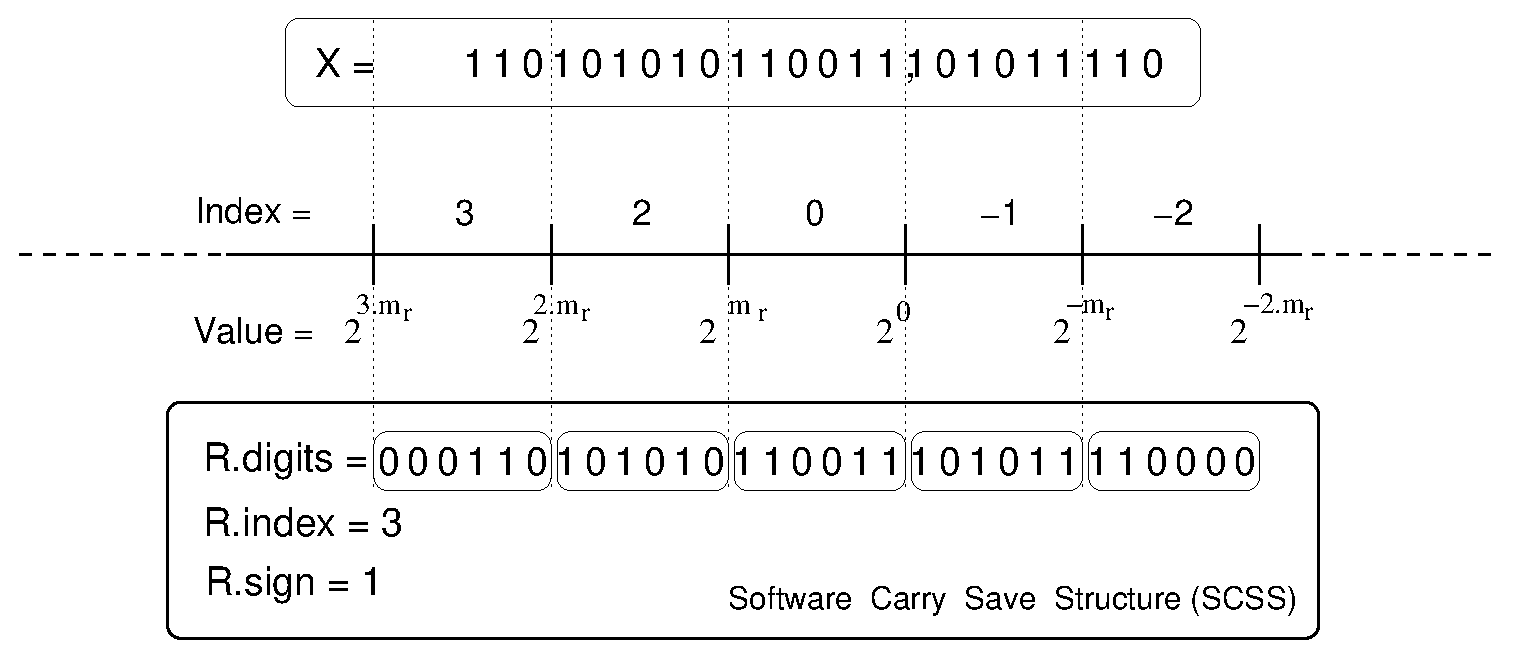
\includegraphics[width=0.7\textwidth]{fig_scs/exponent_representation} % image file name
\caption{The proposed format \label{fig:scsrepresentation}}
\end{center}
\end{figure}
  
In other words, the value  $x$ of a representation $R$  is:
\begin{equation}
\label{eqn4}
x = R.sign \times \sum_{j=1}^{n_r} R.digits[j] \times 2^{m_r * (R.index - j)}
\end{equation}

In such a \emph{normal} SCS number $R$, the bits from $m_I$ to $m_r$
of the $R.digits$ fields are thus set to zero. They will be exploited
by the algorithms to store temporary \emph{carry} information, and are
therefore called \emph{carry-save} bits. An SCS number where these
bits are non-zero is said to be non-normal.

The values of the parameters for use in \crlibm\ is $n_r=8$ digits of
$m_i=30$ bits stored on $m_r=32$-bit words. The worst-case precision
that this format may hold is when the most significant digit is equal
to $1$, meaning that an SCS numbers holds only $1+7\times 30=211$
significant digits.


\subsection{Arithmetic operations\label{sec:ops}}


\subsubsection{Conversion from double to SCS}
 A first method for converting a double precision floating
point number $d$ into an SCS representation is to extract the
exponent $d_{exp}$ from $d$, and then determine the corresponding
$R.index$ as the integer part of
$\frac{d_{exp}}{2^{m_r}}$.

Another method uses a variable number of multiplications by
$2^{m_r}$ or $2^{-m_r}$. This method is faster than the previous one
when the exponent of $d$ is close to $0$.

After testing both methods in \crlibm, the first method was preferred.


\subsubsection{Addition and subtraction}

The addition of two SCS numbers of the same sign consists in aligning,
then adding digits of the same order. Thanks to the carry-save bits,
all these additions will be \emph{exact} and \emph{independent}.
However the result will usually not be a normal SCS number: the sums
will have overflown in the carry-save bits. A \emph{renormalization}
procedure is presented in section \ref{renorm} to propagate these
carry bits and get again a normal SCS number.  However, the advantage
of SCS representation is that many SCS numbers can be summed before
needing to perform this expensive step (up to 7 with the choice of
parameters made in \crlibm).

The subtraction (addition of two numbers of opposite signs) is very
similar to the addition algorithm. It may also classically lead to a
cancellation, which may need an update of the index of the result.
However, as in other floating-point formats, a subtraction involving a
a cancellation is exact.

Although all the digit operations are exact, the addition or
subtraction of two numbers also classically involves a rounding error,
due to aligning the digits of same magnitude. For performance reason
this rounding is a truncation, so the worst-case relative error is one
ulp of the least accurate representable number, or $2^{-211}$.




%---------------- 
% MULTIPLICATION
%----------------
\subsubsection{Multiplication}

The multiplication of two normal SCS numbers involves the operations
depicted on the Figure \ref{fig:scsmultiplication}: The partial
products are computed (in parallel) and summed in columns. The
parameters are set up so that none of these operation overflow. Again,
the result is not a normal SCS number, and a renormalization procedure
(described below) has to be applied to empty the carry bits. However,
a few additions may follow a multiplication before this
renormalization, which allows for further optimization of algorithms
using SCS arithmetic. For instance, a polynomial evaluation can be
implemented with a renormalization after one multiplication and one
addition.

\begin{figure}[h]
\begin{center}
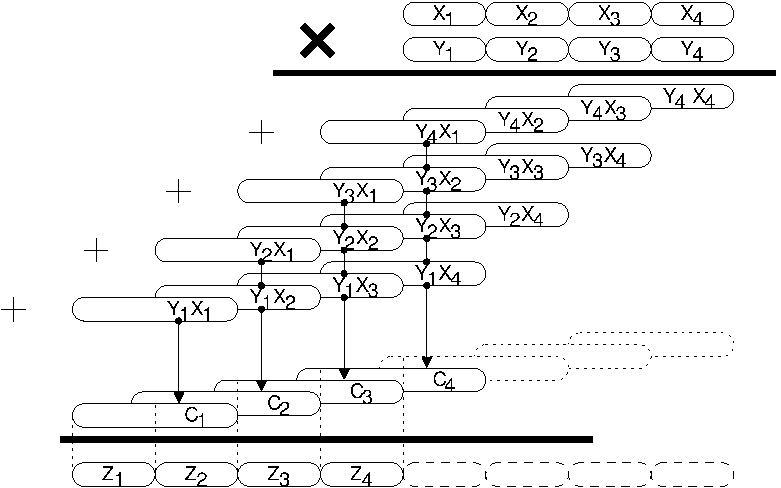
\includegraphics[width=0.7\textwidth]{fig_scs/multiplication}
\caption{SCS multiplication \label{fig:scsmultiplication}}
\end{center}
\end{figure}

Here also, a rounding error is involved when two $n_r$-digit numbers
are multiplied if the result is to fit on $n_r$ digits. The actual
implementation tests if the most significant digit ($z_1$ on
Figure~\ref{fig:scsmultiplication}) is null, in which case the index of
the result is that of $z_2$.

If the whole of the computations of
Figure~\ref{fig:scsmultiplication} are implemented, the worst case
for relative accuracy is again $2^{-211}$. However a further
optimization is to avoid computing the columns of lower magnitude, at
the expense of an increase in the rounding error. More specifically,
we compute 9 columns instead of 16.  The wors case is now when $z_1$
is null, in which case the relative error correspond to the truncation
of the 8 leftmost columns, whose maximum value is smaller than 3 ulps
of the SCS result. Therefore the relative error of the multiplication
is bounded by $2^{-208}$ with this optimization, which is still a
large overkill for the purpose of \crlibm.

This optimization is therefore implemented if the loop are hand-unrolled.
If they are not, the increased control complexity actually degrades
performance.


\subsubsection{Renormalization (carry propagation) \label{renorm}}

Renormalization is a carry propagation from the low order to high
order digits: Starting with an initially null carry, at each step, the
previous carry is added to the current digit, and this sum is then
split into two parts using masks. The low $m_r$ bits are a digit of
the normalized result, and the upper part is the next carry.

The actual algorithm is a little bit more complex. The initial
non-normal number may not be representable exactly as a normal SCS
number, therefore the index of the normalized result may have to be
increased by one or two.  Normalization thus again involves a rounding
error. Note that this error was already taken into account in the previous
discussions of addition and multiplication.




%-----------------
% CONVERSION BACK
%-----------------
\subsubsection{Conversion from SCS to floating-point}

A few (4 in the worst case) multiplications and additions suffice to
get the FP number closest to a SCS number.  For instance, for $m_I=53$
and $m_r=26$, we need to compute $d = A.sign \times 2^{A.index \times
  m_r} \times ( A.digits[0]+ 2^{-m_r} \times A.digits[1]+ 2^{-2.m_r}
\times A.digits[2]+ 2^{-3.m_r} \times A.digits[3])$. The number
$2^{A.index \times m_r}$ is build using integer masks. The actual
implementation of this formula is slightly less simple, but this
conversion is still very fast.


\subsubsection{Mixed 32- and 64-bit arithmetics}

An improvement implemented in \scslib\ was the combined use of integer 32- and 64-bit
arithmetics as follows: 

\begin{itemize}
\item MP digits are stored as 32-bit numbers where only a few bits are
  reserved for carries. This removes the main problem of the initial
implementation \cite{DefDin2002}, namely its memory inefficiency.

\item Addition uses 32-bit arithmetic. 

\item In the MP multiplication, the partial products are products of
  two 32-bit digits, which are 64-bit numbers. The column sums need
  thus to be computed using 64-bit arithmetic. This can be expressed
  in the C language in a non-ISO-C99, but de-facto standard way, as
  follows: 32-bit numbers have the \texttt{unsigned int} type; 64-bit
  numbers have the \texttt{unsigned long long int} type. When
  multiplying two digits, one is first cast into this 64-bit type.
  
  For UltraSPARC architectures (detected at build time) the
  conversion is to floating-point, but we will not detail this
  peculiarity further.
\end{itemize}


This works well because all modern processors either have 64-bit
integer units, or offer instructions which store the 64-bit product of
two 32-bit integers into two 32-bit registers. The compiler does the
rest well, because it is conceptually simple: casting unsigned 32-bit
into unsigned 64-bit is trivial; 64-bit addition is translated
straightforwardly into one 32-bit \emph{add} followed by one 32-bit
\emph{add-with carry}.




\subsubsection{Implementation considerations}

For portability purposes, the implemention uses C as defined by
the ISO C99 standard, and tries to use a recent version of \texttt{gcc}.
We could not exhibit a case where a native compiler from the processor
vendor (Intel or Sun) gave significantly better results than
\texttt{gcc}, which is probably a consequence of the simplicity of our
code.

However, when tuning for performance, we observed that the same code
which was efficient on one processor could lead to very poor results
on another.  Usually, this difference can be traced down to the
capabilities of the processor itself. The typical example is the
knowingly poor integer multiplication on UltraSPARC II. Sometimes
however, the processor should be able to perform well, and it is the
processor-specific backend of the compiler which is to blame, which
can be checked by observing the assembly code produced.  A typical
example is the casting of 32-bits digits to 64-bit arithmetic (or to
an FP number in the case of the UltraSPARC) in the multiplication
algorithm. In these cases we tried to change the programming style in
a way that works well on all processors. Sometimes it wasn't possible,
in which case the code contains, along with a generic version, several
processor-specific tricky versions of the problematic operation,
selected at compile time thanks to the GNU \texttt{automake/autoconf}
tools.


More surprisingly, we were disappointed by the higher-level
capabilities of the compilers, especially at unrolling loops. Our code
exhibits many small \texttt{for} loops whose size is known at
compile-time (usually $n$). This is the ideal situation for loop
unrolling, a technique well known and described in most textbooks on
compiler design. Options exist in most compilers to turn on this
optimisation. Unfortunately, leaving loop unrolling to the compiler
gives very poor results, even when compared to the non-unrolled case.
Since unrolling the loops by hand in the C code takes a few minutes,
we did it for the version of the library which we use ($m=30$, $n=8$).
It marginally increases the code sizes for this small $n$, and
sometimes provides a twofold improvement on speed, depending of the
processor. Of course, this is not satisfactory: We don't want to do it
for all values of $n$, nor do we want to study for each processor the
tradeoffs involved as $n$ increase. We expect however future compilers
to handle unrolling better, and we were surprised that no compiler had
a clear edge on the other in this respect. Some argue, however, that
this issue is pointless, as superscalarity, along with register
renaming and branch prediction inside modern processors, sum up to the
equivalent of dynamic unrolling of the code. In our tests (in 2003), it
doesn't: unrolling does bring a speed-up.








\section{Common Maple procedures \label{section:commonMaple}}


\subsection{Conversions}





Procedure \texttt{ieeedouble} returns the sign, the exponent and the
mantissa of the IEEE-754 double-precision number closest to input
value \texttt{x}.

\begin{lstlisting}[caption={ieeedouble},firstnumber=1]
ieeedouble:=proc(xx)
local x, sgn, logabsx, exponent, mantissa, infmantissa,powermin,powermax,expmin,expmax,expmiddle,powermiddle;
Digits := 100;
x := evalf(xx);
if (x=0) then sgn, exponent, mantissa := 1, -1022, 0
else
  if (x < 0) then sgn := -1
  else sgn := 1
  fi:
  x := abs(x);
  if x >=  2^(1023)*(2-2^(-53)) then mantissa := infinity; exponent := 1023
  else if x <= 2^(-1075) then mantissa := 0; exponent := -1022
      else
         if x <= 2^(-1022) then exponent := -1022
         else
# x is between 2^(-1022) and 2^(1024)
         powermin := 2^(-1022); expmin := -1022;
         powermax := 2^1024; expmax := 1024;
         while (expmax-expmin > 1) do
            expmiddle := round((expmax+expmin)/2);
            powermiddle := 2^expmiddle;
            if x >= powermiddle then
                powermin := powermiddle;
                expmin := expmiddle
            else
                powermax := powermiddle;
                expmax := expmiddle
            fi
          od;
# now, expmax - expmin = 1 and powermin <= x < powermax,
# powermin = 2^expmin and powermax = 2^expmax, so expmin is the exponent of x
         exponent := expmin;
         fi;
         infmantissa := x*2^(52-exponent);
	 if frac(infmantissa) <> 0.5 then mantissa := round(infmantissa)
            else
              mantissa := floor(infmantissa);
               if type(mantissa,odd) then mantissa := mantissa+1 fi
            fi;
         mantissa := mantissa*2^(-52);
      fi;
  fi;
fi;
sgn,exponent,mantissa;
end:
\end{lstlisting}


Procedure \texttt{ieeehexa} returns the hexadecimal representation of the nearest double to its input \texttt{x}.

\begin{lstlisting}[caption={ieeehexa},firstnumber=1]
ieeehexa:= proc(x)
local  hex2, xx, longint, expo, sgn, frac, resultat;
    if(x=0) then resultat:=["00000000","00000000"];
    elif(x=-0) then resultat:=["80000000","00000000"]; # nice try
    else
        xx:=ieeedouble(x);
        sgn:=xx[1]:
        expo:=xx[2]:
        frac:=xx[3]:
        if (expo = -1023) then
            longint := (frac)*2^51 ;   # subnormal
        else
            longint := (frac-1)*2^52 +   (expo+1023)*2^52;
        fi:
        if (sgn=-1) then
            longint := longint + 2^63;
        fi:
        longint := longint + 2^64:  # to get all the hexadecimal digits when we'll convert to string
        hex2:=convert(longint, hex);
        hex2:=convert(hex2, string):

        resultat:=[substring(hex2,2..9), substring(hex2,10..18)]:
    fi:
    resultat;
end proc:
\end{lstlisting}

Procedure \texttt{hexa2ieee} performs the reciprocal conversion.





Procedure \texttt{hi\_lo} returns two IEEE-double numbers $x\_hi$ and
$x\_lo$ so that $x = x\_hi + x\_lo + \epsilon_{-103}$.

\begin{lstlisting}[caption={hi\_lo},firstnumber=1]
hi_lo:= proc(x)
local x_hi, x_lo, res:
x_hi:= nearest(evalf(x)):
res:=x-x_hi:
if (res = 0) then
  x_lo:=0:
else
  x_lo:=nearest(evalf(res)):
end if;
x_hi,x_lo;
end:
\end{lstlisting}
\vspace{0.5cm}




Procedure \texttt{showHowDifficultToRound} takes a real number, and prints
the bits after the 53th of its nearest IEEE floating-point number.


\begin{lstlisting}[caption={showHowDifficultToRound},firstnumber=1]
showHowDifficultToRound:=proc(x)
local xb,xs,s,e,m:
    Digits:=200:
    s,e,m := ieeedouble(x):
    xb:=convert(evalf(x*2^(-e)),binary):
    xs:=convert(xb, string):
    substring(xs,55..153)
end proc:
\end{lstlisting}


\subsection{Procedures for polynomial approximation}


Procedure \texttt{Poly\_exact2} takes in arguments a polynomial
\texttt{P} and a integer \texttt{n}. It returns a truncated
polynomial, of which coefficients are exactly IEEE-double numbers. The
\texttt{n} first coefficients are written over 2 IEEE-double numbers.

\begin{lstlisting}[caption={poly\_exact2},firstnumber=1]
poly_exact2:=proc(P,n)
local deg,i, coef, coef_hi, coef_lo, Q:
Q:= 0:
convert(Q, polynom):
deg:=degree(P,x):
  for i from 0 to deg do
    coef :=coeff(P,x,i):
    coef_hi, coef_lo:=hi_lo(coef):
    Q:= Q + coef_hi*x^i:
    if(i<n) then
        Q := Q + coef_lo*x^i:
    fi:
  od:
  return(Q);
end:
\end{lstlisting}
\vspace{0.5cm}


We also have procedures for computing good truncated polynomial
approximation for a function. As they are useless to the proof, we do
not describe them here, the interested reader is referred to file
\texttt{maple/common-procedures.mpl} for more details.










\subsection{Accumulated rounding error in Horner evaluation
 \label{sec:Horner-maple}}



The following Maple procedures implement the error analysis described
in Section~\ref{sec:Horner}.

Procedure \texttt{compute\_abs\_rounding\_error} computes a bound on
the accumulated rounding error caused by the Horner evaluation of a
truncated polynomial. \texttt{poly} is the polynomial, \texttt{xmax} is the max value of
$|x|$, \texttt{nn} is the degree when \texttt{poly} is computed in double double, and the
first double-double operation is an addition.

This procedure returns the maximum absolute error, and safe bounds on the
minimum and maximum values of the function. It also checks on the fly
that the fast (test-free) versions of the double-double addition can
be used, and prints warnings if it not the case.

\begin{lstlisting}[caption={compute\_abs\_rounding\_error},firstnumber=1]
compute_abs_rounding_error:=proc(poly,xmax, nn)
local n, deg, delta, deltap, i, S, P, Snorm, Smin, Smax, prec:
deltap:=0:
delta:=0:
deg:=degree(poly):

prec:=53; # precision of the first iterations

S:=coeff(poly, x, deg):
Smax:=abs(S):
Smin:=Smax:

if nn<0 then n:=0: else n:=nn: fi:# sometimes called by compute_rel_rounding_error with n=-1

for i from (deg-1) to 0 by -1 do
  P:= convert(S*x, polynom):
  Smin := abs(coeff(poly,x,i)) - xmax*Smax : 
  if(Smin<=0) then 
    printf("Warning! in compute_abs_rounding_error, Smin<=0 at iteration %d, consider decreasing xmax\n",i);
  fi:
  delta:= evalf(xmax*deltap + 2**(-prec)*xmax*Smax):
  if i<n then 
    # fast Add22 ?    
    if abs(coeff(poly,x,i)) < xmax*Smax  # may be improved to xmax*Smax/2
    then printf("WARNING Add22 cannot be used at step %d, use Add22Cond\n" , i  );   
         printf("    coeff=%1.20e,  xmax*Smax=%1.20e"  ,  abs(coeff(poly,x,i)),  xmax*Smax );
    fi:
  fi:
  S:=convert(P+coeff(poly,x,i), polynom):
  Snorm:=evalf(infnorm(S, x=-xmax..xmax)):
  if i=n-1 then prec:=100: fi:  # from the addition of the n-1-th iteration
  deltap:= evalf(delta + 2**(-prec)*(delta + Snorm)): 
  Smax := Snorm + deltap:  
od:
deltap, Smin, Smax;
end proc:
\end{lstlisting}
\vspace{0.5cm}

Procedure \texttt{compute\_rel\_rounding\_error} computes a bound on
the total relative rounding error of a Horner polynomial evaluation,
in the same condition as the previous procedure.

\begin{lstlisting}[caption={compute\_abs\_rounding\_error},firstnumber=1]
compute_rel_rounding_error:=proc(poly,xmax, n)
local deg, p, rho, deltap, Smin, Smax:

deg:=degree(poly):
if(n>0) then p:=100: else p:=53: fi: 

if coeff(poly,x, 0) = 0 then
   deltap, Smin, Smax := compute_abs_rounding_error(poly/x,xmax, n-1):
   rho :=  (2^(-p)*(Smax+deltap) +deltap ) / Smin :
else
   deltap, Smin, Smax := compute_abs_rounding_error(poly,xmax, n):
   rho := deltap /  Smin:
fi:
rho;
end proc:
\end{lstlisting}
\vspace{0.5cm}

Procedures \texttt{compute\_abs\_rounding\_error\_firstmult} and
\texttt{compute\_abs\_rounding\_error\_firstmult} are similar to the
previous, but in the case when the first double-double operation is a
multiplication.



\subsection{Rounding}

Procedure \texttt{compute\_rn\_constant} computes a good constant for
the round-to-nearest test of Theorem~\ref{th:roundingRN1}. Its input
is a bound of the overall relative error of the approximation scheme.




\subsection{Using double-extended}

The file \texttt{maple/double-extended.mpl} contains procedures
similar to those previously described to handle double-extended
precision (64 bits of mantissa and 15 bits of exponent). This is
currently used in experimental code only: The \crlibm\ CVS repository
at \url{http://lipforge.ens-lyon.fr/} contains such code for
exponential and arctangent on Itanium, and arctangent on IA32
processors. For more details see \cite{DinDefLau2004LIP,DinErshGast2005}.




%%% Local Variables: 
%%% mode: latex
%%% TeX-master: "crlibm"
%%% End: 


\chapter{The natural logarithm \label{chap:log}}
There are two versions of the logarithm.
\begin{itemize}
\item The first relies on 80-bit double-extended arithmetic, and is
  well suited to IA32 and IA64 architectures which have hardware
  support for such arithmetic. It computes the quick step in
  double-extended arithmetic, and the accurate step in
  double-double-extended arithmetic.
\item The second relies only on double-precision arithmetic, and is
  portable. It uses double-double for the quick step, and
  triple-double for the accurate step.
\end{itemize}

Both implementations use the same algorithm, which is detailed in
\ref{sec:logoutline}. Sections \ref{sec:logdeproof} and
\ref{sec:logtdproof} detail the proof of both implementations, and
\ref{sec:logperf} give some performance results.


\section{General outline of the algorithm\label{sec:logoutline}}
The algorithm used is mainly due to 
Wong and Goto\cite{WG94} and has been discussed further in \cite{Muller97}. In the case we are given here,
both quick and accurate phase use principally the same algorithm however optimized for different accuracies.

The function's argument $x \in \F$ is first checked for special cases, such as $x\leq0$, $+\infty$, $\nan$ etc.
These checks are mainly implemented using integer arithmetics and will be further explained in section
\ref{subsec:reduction}. Then, the argument is reduced using integer arithmetics as follows:
$$x = 2^{E^\prime} \cdot m$$
where $E^\prime$ is the exponent of $x$ and $m$ a double corresponding
to the mantissa of $x$. This decomposition is done such that in any
case, i.e. even if $x$ is subnormal, $1 \leq m < 2$. In the subnormal
case, the exponent of $x$ is adjusted accordingly.  This first
argument reduction corresponds to the equality
$$\log\left( x \right) = E^\prime \cdot \log\left(2\right) + \log\left(m \right)$$
Using this term directly would lead to catastrophic cancellation in the case where $E^\prime = -1$ and
$m \approx 2$. To overcome this difficulty, a second adjustment is done as follows:
\begin{center}
  \begin{tabular}{cc}
    \begin{minipage}{50mm}
      $$E = \left \lbrace \begin{array}{lcl} E^\prime & \mbox{ if } & m \leq \sqrt{2} \\
          E^\prime +1 & \mbox{ if } & m > \sqrt{2} \end{array} \right.$$
    \end{minipage}
    &
    \begin{minipage}{50mm}
      $$y = \left \lbrace \begin{array}{lcl} m & \mbox{ if } & m \leq \sqrt{2} \\
          \frac{m}{2} & \mbox{ if } & m > \sqrt{2} \end{array} \right.$$
    \end{minipage}
  \end{tabular}
\end{center} 

The decision whether $m \leq \sqrt{2}$ or not is performed using integer arithmetics on 
the high order bits of the mantissa $m$. The test is therefore not completely exact which is no
disadvantage since, in any case, the bound $\sqrt{2}$ is somewhat arbitrary.\par
All the previous reduction steps can be implemented exactly as they consist mainly in decompositions
of a floating point number, multiplications by powers of $2$ and integer additions on the corresponding exponent value.
All this leads to the following equation 
$$\log\left( x \right) = E \cdot \log\left( 2 \right) + \log\left( y \right)$$
where
$$-\frac{1}{2} \cdot \log\left( 2 \right) \leq \log\left( y \right) \leq \frac{1}{2} \cdot \log\left( 2 \right)$$
The magnitude of $y$ is thus still too great for allowing for a direct polynomial approximation of $\log\left(y\right)$.
Therefore, a second argument reduction step is performed using a table of $128$ entries as follows:
using the high order bits of $y$ as an index $i$, a tabulated value $r_i$ is looked up which approximated very well
$\frac{1}{y}$. Setting $z = y \cdot r_i - 1$, one obtains 
$$\log\left( y \right) = \log\left( 1 + z \right) - \log\left( r_i \right)$$
Since $y = \frac{1}{r_i} + \delta$ the magnitude of $z$ is finally
small enough (typically $\left \vert z \right \vert < 2^{-8}$) for
approximating $\log\left(1+z\right)$ by a Remez polynomial
$p\left(z\right)$. The values for $\log\left(r_i\right)$ are of course also tabulated.

It is important to notice that the reduction step 
$$z = y \cdot r_i - 1$$ 
can be implemented exactly which eases the correctness proof of the algorithm. This property will be proven in 
section \ref{subsec:reduction}. The reduced argument $z$ will
be represented as a double-double number $z_\hi + z_\lo$ that will be fed into the polynomial approximation 
algorithms of both quick and accurate phase. Each of these phases will take into account the lower significant value 
$z_\lo$ for more or less 
higher monomial degrees.

Both phases will finally reconstruct the function's value as follows:
$$\log\left( x \right) \approx E \cdot \log\left( 2 \right) + p\left( z \right) - \log\left( r_i \right)$$
using a double (respectively a triple for the accurate phase) double value for each 
$\log\left( 2 \right)$ and $-\log\left( r_i \right)$. The computations necessary for performing this reconstruction
are carried out in double-double arithmetics for the quick phase and triple-double for the accurate phase.

The quick phase uses a modified Remez polynomial of degree $7$ of the form
$$p\left( z \right) = z - \frac{1}{2} \cdot z^2 + z^3 \cdot 
\left( c_3 + z \cdot \left( c_4 + z \cdot \left( c_5 + z \cdot \left( c_6 + z \cdot c_7 \right) \right) \right) \right)$$
with $c_i \in \F$.
This polynomial is evaluated as indicated by the parenthesis in the following term: 
$$p\left( z_\hi + z_\lo \right) \approx \left( \left(z_\hi + z_\lo \right) - \frac{1}{2} \cdot  z_\hi^2\right) + 
\left( \left( - z_\hi \cdot z_\lo \right) + 
\left(z_\hi^2 \cdot z_\hi \right) \cdot 
\left( c_3 + z_\hi \cdot \left( c_4 + z_\hi \cdot \left( c_5 + z_\hi \cdot \left( c_6 + z_\hi \cdot c_7 \right) \right) \right) \right) \right)$$
The mathematical relative approximation error of the polynomial $p\left( z \right)$ defined as
$$\epsilon_{\mbox{\tiny meth}} = \frac{p\left( z \right) - \log\left( 1 + z \right)}{\log\left(1 + z \right)}$$ is bounded by
$$\left \vert \epsilon_{\mbox{\tiny meth}} \right \vert \leq 2^{-62.99}$$
This methodical error is joined by the arithmetical error induced by the evaluation of $p\left( z \right)$ 
and by the rounding of the constants $\log\left( 2 \right)$ and $\log\left( r_i \right)$. 
As will be shown in section \ref{subsec:quickphase}, the overall error of the quick phase defined as
$$\epsilon_{\mbox{\tiny quick}} = \frac{\left(log_\hi + log_\lo\right) - \log\left(x\right)}{\log\left(x\right)}$$
is bounded by
$$\left \vert \epsilon_{\mbox{\tiny quick}} \right \vert \leq 5 \cdot 2^{-65} \leq 2^{-62.6}$$ ~ \par
After the computation of the quick phase double-double value $\left( log_\hi + log_\lo \right)$ a rounding test is performed
using the rounding constants according to \ref{th:roundingRN1}. If the rounding cannot be decided, the accurate 
phase is launched. \par
The accurate phase performs all its computations on the same reduced argument $z = z_\hi + z_\lo$ which will be shown to be 
exact. An approximation polynomial of degree $14$ is used. It is once again a modified Remez polynomial and has the 
following form:
$$p\left( z \right) = z + \frac{1}{2} \cdot z + z^3 \cdot q\left( z \right)$$
where 
$$q\left( z \right) = 
c^\prime_3 + z \cdot \left( 
c^\prime_4 + z \cdot \left( 
c^\prime_5 + z \cdot \left( 
c^\prime_6 + z \cdot \left( 
c^\prime_7 + z \cdot \left( 
c^\prime_8 + z \cdot \left( 
c^\prime_9 + z \cdot r\left( z \right) \right) \right) \right) \right) \right) \right)$$
with
$c^\prime_i = c_{i\hi} + c_{i\lo} \in \F + \F$ and
$$r\left( z \right) = 
c_{10} + z \cdot \left(
c_{11} + z \cdot \left(
c_{12} + z \cdot \left(
c_{13} + z \cdot c_{14} \right) \right) \right)$$
with $c_i \in \F$.
The mathematical relative error 
$$\epsilon_{\mbox{\tiny meth}} = \frac{p\left( z \right) - \log\left( 1 + z \right)}{\log\left( 1 + z \right)}$$
is bounded by
$$\left \vert \epsilon_{\mbox{\tiny meth}} \right \vert \leq  2^{-125}$$
The polynomial is evaluated using double precision for $r\left( z \right)$, double-double arithmetic for
$q\left( z \right)$ and a triple-double representation for $p\left( z \right)$ and the final reconstruction.

The overall error 
$$\epsilon_{\mbox{\tiny accurate}} = \frac{\left( log_\hi + log_\mi + log_\lo \right) - \log\left( x \right)}{\log\left( x \right)}$$
is bounded by 
$$\left \vert \epsilon_{\mbox{\tiny accurate}} \right \vert \leq 5735 \cdot 2^{-132} \leq 2^{-119.5}$$
as will be shown in section \ref{subsec:accuratephase}. Here $\left( log_\hi + log_\mi + log_\lo \right)$ 
are obtained by reconstructing the logarithm as indicated by the parenthesis in the following term:
$$log_\hi + log_\mi + log_\lo = \left(E \cdot \left( log2_\hi + log2_\mi + log2_\lo \right) \right) + 
\left( \left( p_\hi + p_\mi + p_\lo \right) + \left(logi_\hi + logi_\mi + logi_\lo \right) \right)$$
where
$log2_\hi + log2_\mi + log2_\lo \approx \log\left( 2 \right)$ and $logi_\hi + logi_\mi + logi_\lo \approx -\log\left(r_i \right)$.

Since the critical accuracy of the double precision $\log$ function is $118$ bits according to 
\cite{DinDefLau2004LIP}, rounding $\log_\hi + log_\mi + log_\lo \approx \log\left( x \right)$ to double precision is equivalent 
to rounding the infinite precision value $\log\left( x \right)$ to double precision. 
Using the final rounding sequences presented in \cite{Lauter2005LIP:tripledouble}, which are supposed to be correct, 
the double precision value returned by the function is the correctly rounded double precision value of 
$\log\left( x \right)$.



\section{Proof of correctness of the triple-double implementation \label{sec:logtdproof}}
Proving that an implementation of an elementary function is correctly rounded means mainly proving two 
bounds on the relative error $\epsilon_{\mbox{\tiny quick}}$ and $\epsilon_{\mbox{\tiny accurate}}$, using the appropriate lemma for proving the
correctness of the rounding test and conluding by means of the theorem stating the critical accuracy of the 
function considered. The computation of the error bounds will be done mainly using the Gappa tool\cite{Melqu05} but
some parts of the proof are still based on paper or Maple computations. These parts will be shown in sections 
\ref{subsec:reduction}, \ref{subsec:quickphase} and \ref{subsec:accuratephase} and mainly comprise the following:
\begin{itemize}
\item the demonstration that all special cases are handled correctly, 
\item a proof that $z_\hi + z_\lo = r_i \cdot y - 1$ exactly,
\item the bounds for the mathematical approximation errors for the polynoms,
\item a proof of the exactness of some multiplications in the code,
\item the proof for the accuracy of all basic addition and multiplication code sequences on 
double-double and triple-double numbers,
\item the correctness proof of the final rounding sequences for rounding triple-double numbers to double precision and
\item the mathematical equality of the term rewriting hints in the Gappa code.
\end{itemize}
The proofs for the accuracy of the basic operation bricks and the correctness proof of the final rounding sequences
are somewhat lengthy and are not given here; they can be found in \cite{Lauter2005LIP:tripledouble}.
\subsection{Exactness of the argument reduction\label{subsec:reduction}}
In this section, we will show that all special cases are handled correctly and that the 
reduced argument consisting in $E$ and $z_\hi + z_\lo$ is exact, which means that we have the mathematically exact 
equation
$$\log\left( x \right) = E \cdot \log\left( 2 \right) + \log\left( 1 + \left( z_\hi + z_\lo \right) \right) - \log\left( r_i \right)$$
This part of the algorithm is performed by the following code sequences which we will analyse line by line:
\begin{lstlisting}[caption={Handling of special cases and table access},firstnumber=1]
E=0;
xdb.d=x;

/* Filter cases */
if (xdb.i[HI] < 0x00100000){                     /* x < 2^(-1022)    */
  if (((xdb.i[HI] & 0x7fffffff)|xdb.i[LO])==0){
    return -1.0/0.0;     
  }                    		                 /* log(+/-0) = -Inf */
  if (xdb.i[HI] < 0){ 
    return (x-x)/0;                              /* log(-x) = Nan    */
  }
  /* Subnormal number */
  E = -52; 		
  xdb.d *= ((db_number) ((double) two52)).d; 	 /* make x a normal number    */ 
}
    
if (xdb.i[HI] >= 0x7ff00000){
  return  x+x;				         /* Inf or Nan       */
}
     

/* Do argument reduction */
E += (xdb.i[HI]>>20)-1023;                       /* extract the exponent */
index = (xdb.i[HI] & 0x000fffff);
xdb.i[HI] =  index | 0x3ff00000;	         /* do exponent = 0 */
index = (index + (1<<(20-L-1))) >> (20-L);
 
/* reduce  such that sqrt(2)/2 < xdb.d < sqrt(2) */
if (index >= MAXINDEX){                          /* corresponds to xdb>sqrt(2)*/
  xdb.i[HI] -= 0x00100000; 
  E++;
}
y = xdb.d;
index = index & INDEXMASK;

ed = (double) E;

ri = argredtable[index].ri;

logih = argredtable[index].logih;
logim = argredtable[index].logim;
\end{lstlisting}
Analysis of the code: 
{\renewcommand{\labelenumi}{}
\begin{enumerate}
\item line 1 and 2: Initialization of integer $E$ and {\tt db\_number} {\tt xdb} which is now equal to $x$.
\item line 5: As the integer ordering and the ordering on floating point numbers are compatible, 
$x < +2^{-1022}$, i.e. negative, negative infinite, equal to zero or a subnormal. 
\item line 6: {\tt xdb.i[HI] \& 0x7fffffff} is the high order word of $x$ without the sign bit. If the test is true,
$\left \vert x \right \vert = 0$. As the logarithm of $0$ is not defined but as the limit $-\infty$ is known, returning
$-1.0 / 0.0$ is correct.
\item line 9: Since the integer ordering and the ordering on floating point numbers are compatible, 
{\tt xdb.i[HI] < 0} implies $x < 0$. The logarithm is not defined for negative numbers, so the result must be $\nan$. 
$0.0 / 0.0$ leads to a $\nan$; one uses $\left(x - x\right) / 0.0$ in order to overcome the static tests of the compiler.
\item line 13 and 14: if this code lines are reached, $x$ is a subnormal. Since $E$ equals $0$ at this point, 
setting it to $-52$ and multipliying {\tt xdb} by $2^{-52}$ means bringing {\tt xdb} to the normal number range and
rescaling the internal representation $x = 2^E \cdot m = 2^E \cdot${\tt xdb} in consequence.
\item line 17: As the integer ordering and the ordering on floating point numbers are compatible and as 
{\tt 0x7fefffff ffffffff} is the greatest normal, the test being true implies that $x$ is equal to $+\infty$ or $\nan$.
In the case of $x=+\infty$, $+\infty$ must be returned which is done. In the other case, $\nan$ must be returned which is
still assured by $x + x$.
\item line 23: At this point of the code, the most significant bit of the high order word of {\tt xdb} must be $0$ as
the case where $x < 0$ is already filtered out. So {\tt xdb.i[HI] > > 20} is equal to the biased exponent of {\tt xdb} 
because a double number consists in $1$ sign bit, $11$ exponent bits and the word bit length is supposed to be $32$. 
Subtracting $1023$ yields to the unbiased exponent which is written to $E$.
\item line 24 and 25: Since a double number consists in $1$ sign bit and $11$ exponent bits, the operation 
{\tt xdb.i[HI] \& 0x000fffff} masks out the mantissa bits in the higher order word of {\tt xdb}. 
Rewriting {\tt xdb.i[HI] = index | 0x3ff00000} means setting the exponent of {\tt xdb} to $0$ because 
{\tt 0x3ff}$ - 1023 = 0$. 
\item line 26: Before execution of this line of code, {\tt index} contains the high order bits of the normalized mantissa
of $x$ stored as a double in {\tt xdb.d} and verifying thus $1 \leq m < 2$. The second argument reduction step
will slice this intervall in $128$ intervalls for each of which we dispose of a table entry. For reasons of possible 
cancellation in the reconstruction step on the operation $p\left( z \right) - \log\left( r_i \right)$, we want the 
small intervalls to be centered around $1$. That means e.g. for the intervall around $1$ and a table indexed by $7$ bits
that mantissas (as doubles) with the high order word {\tt 0x3fefffff} through {\tt 0x3ff00fff} must be mapped to $0$.
The decision is therefore made at the $7+1$th bit of the mantissa part of the double depending on whether this bit is $0$ 
-- in which case the value falls in the lower intervall -- or $1$ -- in which case the value goes to the next higher 
intervall. So adding $1$ to the $\left(20 - 7 - 1\right)$ rightmost bit ($L = 7$) increases the index value by $1$ iff this bit is $1$.
So after execution of the line, {\tt index} contains the number of the intervall for the second argument reduction step 
centered in $1$.
\item line 29 through 31: The second adjustment to be made on $E^\prime$ and $m$ is the decision whether $m > \sqrt{2}$ as
indicated in section \ref{sec:logoutline}. The high order word of $\sqrt{2}$ rounded to a double is {\tt 0x3ff6a09e}.
As one can simply verify, the value for {\tt index} calculated for this value is $53$. As the integer ordering and 
the ordering of floating point numbers are compatible and as the computations for computing {\tt index} are monotone,
{\tt index} being greater or equal than $53$ implies that the (normalized) mantissa of $x$ is greater than 
$\sqrt{2} + \delta$ with a neglectable error $\delta$. 
As {\tt MAXINDEX} is equal to $53$, the test will be true iff the adjustment on $E^\prime$ leading
to $E$ and $m$ yielding $y$ is to be made. It is trivial to see that the code in the {\tt if}'s body implements the
adjustment correctly.
\item lines 33 and 34: the final value of the reduced argument $y$ -- still stored in {\tt xdb.d} -- is copied to 
a {\tt double} variable (or register) named {\tt y}. The final index value is masked out by means of an {\tt INDEXMASK}
which is equal to $127 = 2^7-1$.
\item lines 36: The integer value of the exponent $E$ stored in {\tt E} is cast to a {\tt double ed}.
\item lines 38 through 41: The table is indexed by {\tt index} and values {\tt ri}$=r_i$ and 
{\tt logih}$=logi_\hi$ and {\tt logim}$=logi_\mi$ are read. 
Since the latter form a double-double precision value, we know that 
$logi_\hi + logi_\mi = \log\left( r_i \right) \cdot \left( 1 + \epsilon \right)$ with $\left \vert \epsilon \right \vert \leq 2^{-106}$.
The value {\tt ri} is stored as a single precision variable and a Maple procedure assures that for each value
$y$ the following inegality is verified:
$$\left \vert z \right \vert = \left \vert y \cdot r_i - 1 \right \vert \leq 2^{-8}$$
\end{enumerate}
} 
Let us show now that the following line calculate $z_\hi$ and $z_\lo$ such that for each $y$ and corresponding $r_i$,
we obtain exactly
$$z_\hi + z_\lo = y \cdot r_i - 1$$
\begin{lstlisting}[caption={Argument reduction},firstnumber=42]
Mul12(&yrih, &yril, y, ri);
th = yrih - 1.0; 
Add12Cond(zh, zl, th, yril); 
\end{lstlisting}
We know that we can suppose that the multiplication and addition sequences \Mul~ and \Add~ used at lines
42 and 44 are exact. Thus, it suffices to show that
$$yri_\hi - 1.0 = yri_\hi \ominus 1.0$$
because in that case, we can note
$$z_\hi + z_\lo = th + yri_\lo = yri_\hi \ominus 1.0 + yri_\lo = y \cdot r_i - 1.0$$
We will show this property using Sterbenz' lemma. It suffices thus to prove that
$$\frac{1}{2} \leq yri_\hi \leq 2$$
We know that 
\begin{eqnarray*}
yri_\hi & = & \circ\left( y \cdot r_i \right) \\
& \leq & \circ \left( 1 + 2^{-8} \right) \\
& = & 1 + 2^{-8} \\
& < & 2
\end{eqnarray*}
since the rounding function $\circ$ is monotonic and the accuracy of the format is greater than $9$ bits.

The other way round, we get
\begin{eqnarray*}
yri_\hi & = & \circ \left( y \cdot r_i \right) \\
& \geq & \circ \left( 1 - 2^{-8} \right) \\
& = & 1 - 2^{-8} \\
& > & \frac{1}{2}
\end{eqnarray*}
for the same reasons.

Thus $z_\hi + z_\lo = y \cdot r_i$ exactly. Since the previous phases of the argument reduction were all exact, the reduced argument
verifies $x = 2^{E} \cdot y$ exactly.

Still in this section, let us show that neither the reduced argument of the logarithm function nor its result may be
a sub-normal double number. The first property has already been assured by special case handling as shown above. The 
latter can be proven as follows: the $\log\left( x \right)$ function has one zero for $x = 1$ and only one. 
As it is monotone, for $x = 1 \pm 1 \mUlp = 1 \pm 2^{-52}$ we will obtain $\log\left( 1 \pm 2^{-52} \right) = 0 \pm 2^{-52} + \delta$ 
with 
$\left \vert \delta \right \vert \leq 2^{-103}$. As $0 \pm 2^{-1022}$ is the least normal, the result of the logarithm function will
always be a normal. Further, in both double-double and triple-double representations for the final intermediate result
for the function, as its critical accuracy is $118$, the least significant double in the representation will still be
a normal as $52 + 106 = 158 < 1022$. 
\subsection{Accuracy proof of the quick phase\label{subsec:quickphase}}
As already mentionned, the accuracy proof of the quick phase is mainly based on the Gappa tool. To prove the desired
accuracy bound defined as
$$\epsilon_{\mbox{\tiny quick}} = \frac{\left(log_\hi + log_\lo\right) - \log\left(x\right)}{\log\left(x\right)}$$ 
and given by
$$\left \vert \epsilon_{\mbox{\tiny quick}} \right \vert \leq 5 \cdot 2^{-65} \leq 2^{-62.6}$$ 
three different Gappa proof files are necessary depending on the following cases: 
\begin{itemize}
\item for $E \geq 1$ and all indexes to the table $0 \leq i \leq 127$, a general proof file named {\tt log-td.gappa} is used
\item for $E = 0$ and all indexes to the table except $0$, i.e. $1 \leq i \leq 127$, a proof file named {\tt log-td-E0.gappa}
comes to hand and
\item for $E = 0$ and the table index $i = 0$, a proof file called {\tt log-td-E0-logir0.gappa} is employed. 
This latter file
uses relative error computations in opposition to the other two cases where absolute error estimates suffice. This
is necessary because in this case and in this one only, the logarithm function has a zero in the intervall considered.
\end{itemize}
In each of the three proof files, we will ask the Gappa tool to verify the accuracy bound expressed in its syntax as
follows:
\begin{lstlisting}[caption={Accuracy bound to prove},firstnumber=109]
->
((logh + logm) - Log) / Log in [-5b-65,5b-65]
\end{lstlisting}
Still in any proof file, some hypothesis are made on the correctness of one multiplication sequence and the
accuracy of the constants and resting operations carried out in double-double arithmetic.
These hypothesis are the following:
\begin{itemize}
\item The operations in the following code sequence are exact since the constants are stored with enough trailing zeros:
\begin{lstlisting}[caption={Multiplication by $E$},firstnumber=50]
Add12(log2edh, log2edl, log2h * ed, log2m * ed);
\end{lstlisting}
This means that $log2ed_\hi + log2ed_\lo = E \cdot \left( log2_\hi + log2_\lo \right)$ exactly.
\item The operations in the following code sequence are exact since multiplications with a power of $2$ are exact
as long as the result is not underflowed:
\begin{lstlisting}[caption={Multiplication by $-0.5$},firstnumber=60]
zhSquareHalfh = zhSquareh * -0.5;
zhSquareHalfl = zhSquarel * -0.5;
\end{lstlisting}
i.e. $zhSquareHalf_\hi + zhSquareHalf_\lo = -0.5 \cdot \left( zhSquare_\hi + zhSquare_\lo \right)$.
\item The following hypothesis on the accuracy bounds, expressed here in Gappa syntax, are verified:
\begin{lstlisting}[caption={Gappa hypothesis},firstnumber=100]
(T2hl - T2) / T2 in [-1b-103,1b-103]
/\ (Phl - PE) / PE in [-1b-103,1b-103]
/\ (LogTabPolyhl - LogTabPoly) / LogTabPoly in [-1b-103,1b-103]
/\ (Loghm - LogE) / LogE in [-1b-103,1b-103]
/\ (Log2hm - Log2) / Log2 in [-1b-84,1b-84]
/\ (Logihm - Logir) / Logir in [-1b-106,1b-106]
/\ Z in [_zmin,_zmax]
/\ (P - Log1pZ) / Log1pZ in [-_epsilonApproxQuick,_epsilonApproxQuick]
/\ ((logh + logm) - Loghm) / Loghm in [-1b-106,1b-106]
\end{lstlisting}
Here, {\tt \_zmin}, {\tt \_zmax} and {\tt \_epsilonApproxQuick} are replaced by Maple calculated values, typically
$-zmin = zmax = 2^{-8}$ and $epsilonApproxQuick = 2^{-62.99}$.
\end{itemize}
Let us now show each of this hypothesises. 
\begin{enumerate}
\item The operations yielding {\tt log2edh} and {\tt log2edl} are all exact because the \Add~ sequence is supposed 
to be exact in any case and because the constants {\tt log2h} and {\tt log2m} are calculated by the following Maple
code and have in consequence at least 11 trailing zeros and {\tt ed} $=E$ is less than $1024$ in magnitude since $1024$ is
the maximum exponent value for double precision. 
\begin{lstlisting}[caption={Maple code for computing {\tt log2h} and {\tt log2m}},firstnumber=21,label={list:maplelog2}]
log2acc := log(2):
log2h := round(log2acc * 2**(floor(-log[2](abs(log2acc))) + (53 - 11))) / 
         2**(floor(-log[2](abs(log2acc))) + (53 - 11)):
log2m := round((log2acc - log2h) * 2**(floor(-log[2](abs((log2acc - log2h)))) + 
         (53 - 11))) / 2**(floor(-log[2](abs((log2acc - log2h)))) + (53 - 11)):
\end{lstlisting}
\item To show that $zhSquareHalf_\hi + zhSquareHalf_\lo = -0.5 \cdot \left( zhSquare_\hi + zhSquare_\lo \right)$ we just have to show
that both values $zhSquare_\hi$ and $zhSquare_\lo$ are either equal to $0$ or greater than $2$ times the smallest
normal. Let us first give the definitions of both values:
\begin{eqnarray*}
zhSquare_\hi & = & \circ \left( z_\hi \cdot z_\hi \right) \\
zhSquare_\lo & = & z_\hi \cdot z_\hi - zhSquare_\hi 
\end{eqnarray*}
where $z_\hi = \circ \left( z \right)$.
Let us suppose that $z \not = 0$. Otherwise all values are equal to $0$ and we can conclude.

Let us first show that $\left \vert zhSquare_\hi \right \vert$ is greater than $2^{54}$ times the smallest normal. 
Let us therefore suppose that this
is not the case, i.e. $\left \vert zhSquare_\hi \right \vert < 2^{-948}$. Since the rounding function is monotonic,
this implies that $\left \vert z_\hi \right \vert \leq 2^{-424}$. For the same reason, we can note that 
$\left \vert z \right \vert \leq 2^{-424}$. As we have $z = y \cdot r_i - 1$, clearly neither $y$ nor $r_i$ can be exactly $1$. 
If this were the case for both, we would obtain $z=0$ which we excluded; if there were one of them only that was
exactly $1$, the other being a floating point number in the intervall $\left[ 0.5; 1.5 \right]$, 
the resulting inegality $\left \vert z \right \vert \geq 2^{-53}$ which would be contradictory.

Otherwise, since we know that $1 - 2^{-8} \leq y \cdot r_i \leq 1 + 2^{-8}$ and since the precision of all formats used is greater than 
$9$, the hypothesis that $1 - 2^{-424} \leq y \cdot r_i \leq 1 + 2^{-424}$ and $y \cdot r_i \not = 0$ 
would imply that the infinite precision mantissa of 
$y \cdot r_i$ contains a $1$ weighted with $2^0$ and a $1$ weighted with less than $2^{-424}$. So its length would be greater than
$423$ bits. As it is the product of two floating point numbers which have $52$ and $23$ significant bits, there
cannot be a $1$ weighted with less than $76$ if there is a $1$ weighted with $2^0$ which is the case. Contradiction. 

So $-0.5 \cdot zhSquare_\hi$ is not underflowed. Additionally, with a similar argument, since {\tt zh} is a double precision
number, $zhSquare_\lo$ is either $0$ or greater in magnitude than $2^{-53} \cdot \left \vert zhSquare_\hi \right \vert$ which is
$2^{52}$ times greater in magnitude than the smallest normal. So $zhSquare_\lo$ is either $0$ or $2$ times greater in
magnitude than the smallest normal. 

So, the floating point multiplication of $zhSquare_\hi$ and $zhSquare_\lo$ with $-0.5$ can be considered to be exact.
\item {\tt (T2hl - T2) / T2 in [-1b-103,1b-103]} which means that 
$$\left \vert \frac{T2hl - T2}{T2} \right \vert \leq 2^{-103}$$ is verified as $T2hl$ and $T2$ are defined as follows:
$$T2hl = t2_\hi + t2_\lo \gets \mAddDD \left( z_\hi, z_\lo, zhSquareHalf_\hi, zhSquareHalf_\lo \right)$$
$$T2 = \left( z_\hi + z_\lo \right) + \left( zhSquareHalf_\hi + zhSquareHalf_\lo \right)$$
The given bound is thus just the accuracy bound of the \AddDD~ sequence for which a proof can be found in 
\cite{Lauter2005LIP:tripledouble}.
\item {\tt (Phl - PE) / PE in [-1b-103,1b-103]} is verified for the same reason; let us just recall the definitions
$$Phl = p_\hi + p_\lo \gets \mAddDD \left( t2_\hi, t2_\lo, t1_\hi, t1_\lo \right)$$
$$PE = \left( t2_\hi + t2_\lo\right) + \left( t1_\hi + t1_\lo \right)$$
\item {\tt (LogTabPolyhl - LogTabPoly) / LogTabPoly in [-1b-103,1b-103]} falls still into the same case with
$$LogTabPolyhl = logTabPoly_\hi + logTabPoly_\lo \gets \mAddDD \left( logi_\hi, logi_\mi, p_\hi, p_\lo \right)$$
$$LogTabPoly = \left( logi_\hi, + logi_\mi \right) + \left( p_\hi +  p_\lo \right)$$
\item And finally, {\tt (Loghm - LogE) / LogE in [-1b-103,1b-103]}
which is also just the accuracy bound of the \AddDD~ sequence for 
$$Loghm = log_\hi + log_\mi \gets \mAddDD \left( log2ed_\hi, log2ed_\lo, logTabPoly_\hi, logTabPoly_\lo \right)$$
$$LogE = \left( log2ed_\hi + log2ed_\lo \right) + \left( logTabPoly_\hi + logTabPoly_\lo \right)$$
\item {\tt (Log2hm - Log2) / Log2 in [-1b-84,1b-84]} is verified 
since $log2_\hi$ and $log2_\mi$ are computed as already indicated in listing \ref{list:maplelog2}.
This means that at least $11$ trailing zeros are stored in each in the doubles in this (pseudo-)double-double number, 
so it is exact to $2^{-106-2 \cdot 11} = 2^{-84}$.
\item {\tt (Logihm - Logir) / Logir in [-1b-106,1b-106]} which means
$$\left \vert \frac{\left( logi_\hi + logi_\mi \right) - \log\left( r_i \right)}{\log\left( r_i \right)} \right \vert \leq 2^{-106}$$
is verified by construction as $logi_\hi$ and $logi_\mi$ are computed by the following Maple code:
\begin{lstlisting}[caption={Maple code for computing $logi_\hi$ and $logi_\mi$},firstnumber=35]
(logih[i], logim[i], logil[i]) := hi_mi_lo(evalf(-log(r[i]))):
\end{lstlisting}
where {\tt hi\_mi\_lo} is the procedure for rounding an arbitrary precision number to a triple-double number the higher
significant numbers of which form a double-double number.
\item The hypothesis {\tt Z in [\_zmin,\_zmax]} simply recalls the bounds for $z$ as calculated by Maple.
\item The same can be said on the hypothesis \\
{\tt (P - Log1pZ) / Log1pZ in [-\_epsilonApproxQuick,\_epsilonApproxQuick]} \\
which gives the mathematical approximation error of the polynomial. This bound is computed by Maple using the following
instructions:
\begin{lstlisting}[caption={Maple code for computing the relative error of the polynomial},firstnumber=129]
epsilonApproxQuick := numapprox[infnorm]( 1-polyQuick/log(1+x), x=zminmin..zmaxmax)
\end{lstlisting}
\item Finally, Gappa's hypothesis {\tt ((logh + logm) - Loghm) / Loghm in [-1b-106,1b-106]} 
simply restates the fact that a double-double precision number is exact to 
at least $2^{-106}$ in terms of its relative error.
\end{enumerate}
The Gappa tool itself is not capable of proving the final accuracy bound it is asked for a complex algorithm as the 
one given here. Its user must provide hints to help it to rewrite the interval arithmetics terms it encounters
in the program. These hints are generally given in the form {\tt $\alpha$ -> $\beta$} 
where $\beta$ is an expression we want the
tool to rewrite the expression $\alpha$ by. Generally speaking, the idea behind each hint is one of the following:
\begin{itemize}
\item For computing intervall bounds on differences like $\alpha = a - A$ where both $a$ and $A$ are sums of terms like 
$a = c + C$ and $B = d + D$, it is often useful to rewrite $\alpha$ by $\beta = \left(c - d \right) + \left( C - D \right)$.
\item An intervall bound can often be easier found for a term $A$ representing an exact mathematical value that for $a$
which is its arithmetical equivalent. So it is useful to rewrite $a$ by $A \cdot \left( 1 + \frac{a - A}{A} \right)$ when 
an intervall for $\frac{a - A}{A}$ is known. 
\item Fractional left hand sides like $\frac{a}{b}$ where both expressions $a$ and $b$ are functions in a common argument
$x$ that can be written like $a = a\left( x \right) = x^n \cdot a^\prime\left( x \right)$ and 
$b = b\left( x \right) = x^m \cdot b^\prime\left( x \right)$ should usually be rewritten as follows:
$$\frac{a\left(x\right)}{b\left( x \right)} = \frac{x^n \cdot a^\prime\left( x \right)}{x^m \cdot b^\prime\left( x \right)} = 
x^{n - m} \cdot \frac{a^\prime\left( x \right)}{b^\prime\left( x \right)}$$ In particular, this kind of hint is needed when an 
intervall for the denominator of a fractional left-hand-side comprises $0$.
\item Fractional left-hand-sides of the form $\frac{a - A}{A}$ with an unknown $A$ can easily be written like
$$\frac{a - A}{A} = \frac{a - B}{B} + \frac{B - A}{A} + \frac{a - B}{B} \cdot \frac{B - A}{A}$$
We can show this equivalence like this
\begin{eqnarray*}
\frac{a - A}{A} & = & \frac{a - B + B - A}{A} \\
& = & \frac{a - B}{A} + \frac{B - A}{A} \\
& = & \frac{a - B}{B} \cdot \frac{B}{A} + \frac{B - A}{A} \\
& = & \frac{a - B}{B} \cdot \left( 1 + \frac{B - A}{A} \right) + \frac{B - A}{A} \\
& = & \frac{a - B}{B} + \frac{B - A}{A} + \frac{a - B}{B} \cdot \frac{B - A}{A}
\end{eqnarray*}
This is particularly useful when a bound on the relative error of some term $a$ with regard to $B$ should be 
extended to the next approximation level. 
\end{itemize}
Clearly, the left-hand-side $A$ and right-hand-side $B$ of an hint must be mathematically equivalent to provide a 
correct result. The Gappa tool checks for this equivalence and sometimes is able to prove it. If not, it emits a
warning indicating that the formal proof it is generating for the accuracy bound computations is valid only under
the hypothesis that both sides of the rewriting hint are mathematically equivalent. Further, it prints out the 
difference $A - B$ of both sides $A$ and $B$ which it has already reduced using the equivalences given in the 
Gappa code. It is relatively simple to verify that all this differences are equal to $0$ modulo the definitions 
given in the Gappa code by means of Maple-scripts. This work can even been done automatically. Thus, we refrain 
from giving a paper proof of each hint in the Gappa files used for proving the logarithm function but just 
give the exhaustive list of the hints in files {\tt log-td.gappa} and {\tt log-td-E0-logir0.gappa}:
\begin{lstlisting}[caption={Gappa term rewriting hints in file {\tt log-td.gappa}},firstnumber=115]
T2hl - T2 -> ((T2hl - T2) / T2) * T2;
T2hl -> (T2hl - T2) + T2;

Phl - PE -> ((Phl - PE) / PE) * PE;
Phl -> (Phl - PE) + PE;


LogTabPolyhl -> (LogTabPolyhl - LogTabPoly) + LogTabPoly;

Loghm -> (Loghm - LogE) + LogE;

Log2 -> Log2hm * (1 / (((Log2hm - Log2) / Log2) + 1));

Logir -> Logihm * (1 / (((Logihm - Logir) / Logir) + 1));


LogTabPolyhl - LogTabPoly -> ((LogTabPolyhl - LogTabPoly) / LogTabPoly) * LogTabPoly;

HZZsimp -> (-0.5 * zh * zh) - (0.5 * zl * zl);

T2hl - ZpHZZsimp -> (0.5 * zl * zl) + delta1;

zhCube - ZZZ -> (Z * (zhSquareh - Z * Z)) - (zl * zhSquareh);

polyUpper - ZZZPhigher -> ZZZ * (polyHorner - Phigher) + polyHorner * delta3 + delta2;

ZpHZZ + ZZZPhigher -> ZpHZZsimp + ZZZPhigherPzhzl;

Phl - P -> (T2hl - ZpHZZsimp) + (T1hl - ZZZPhigherPzhzl) + delta4;

Log1pZ -> P * (1 / (((P - Log1pZ) / Log1pZ) + 1));
P - Log1pZ -> ((P - Log1pZ) / Log1pZ) * Log1pZ;

Phl - Log1pZ -> (Phl - P) + delta6;

LogTabPolyhl - Log1pZpTab -> (Logihm - Logir) + (Phl - Log1pZ) + delta7;

Loghm - Log -> (Log2edhm - Log2E) + (LogTabPolyhl - Log1pZpTab) + delta5;

(logh + logm) - Loghm -> (((logh + logm) - Loghm) / Loghm) * Loghm;

(logh + logm) - Log -> ((logh + logm) - Loghm) + (Loghm - Log);
\end{lstlisting}
\begin{lstlisting}[caption={Gappa term rewriting hints in file {\tt log-td-E0-logir0.gappa}},firstnumber=81]
T2hl - T2 -> ((T2hl - T2) / T2) * T2;
T2hl -> (T2hl - T2) + T2;

Phl - PE -> ((Phl - PE) / PE) * PE;
Phl -> (Phl - PE) + PE;


(ZhSquarehl - ZZ) / ZZ -> 2 * ((zh - Z) / Z) + ((zh - Z) / Z) * ((zh - Z) / Z);

(zhSquareh - ZZ) / ZZ -> ((ZhSquarehl - ZZ) / ZZ) + ((zhSquareh - ZhSquarehl) / ZZ);

(zhSquareh - ZhSquarehl) / ZZ -> ((zhSquareh - ZhSquarehl) / ZhSquarehl) * (ZhSquarehl / ZZ);

ZhSquarehl / ZZ -> ((ZhSquarehl - ZZ) / ZZ) + 1;

(ZhCube - ZZZ) / ZZZ -> (((zh * zhSquareh) - ZZZ) / ZZZ) + ((ZhCube - (zh * zhSquareh)) / ZZZ);

((zh * zhSquareh) - ZZZ) / ZZZ -> (1 + ((zh - Z) / Z)) * (1 + ((zhSquareh - ZZ) / ZZ)) - 1;

((ZhCube - (zh * zhSquareh)) / ZZZ) -> ((ZhCube - (zh * zhSquareh)) / (zh * zhSquareh)) * (((zh - Z) / Z) + 1) * (((zhSquareh - ZZ) / ZZ) + 1);

polyHorner / Phigher -> ((polyHorner - Phigher) / Phigher) + 1;

(polyUpper - ZZZPhigher) / ZZZPhigher -> ((polyHorner - Phigher) / Phigher) + ((ZhCube - ZZZ) / ZZZ) * (polyHorner / Phigher) + 
					  + ((polyUpper - (polyHorner * ZhCube)) / (polyHorner * ZhCube)) * (polyHorner / Phigher) +
					  + ((ZhCube - ZZZ) / ZZZ) * ((polyUpper - (polyHorner * ZhCube)) / (polyHorner * ZhCube)) * 
					    (polyHorner / Phigher);


((ZhSquareHalfhl - (zh * zl)) - HZZ) / HZZ -> - ((zh - Z) / Z) * ((zh - Z) / Z);

(ZhSquareHalfhl - HZZ) / HZZ -> (ZhSquarehl - ZZ) / ZZ;

((T2hl - (zh * zl)) - ZpHZZ) / ZpHZZ -> ((HZ * (((ZhSquareHalfhl - (zh * zl)) - HZZ) / HZZ)) + ((T2hl - T2) / T2) 
                                        + (HZ * ((T2hl - T2) / T2)) 
					+ (HZ * ((ZhSquareHalfhl - HZZ) / HZZ) * ((T2hl - T2) / T2))) / (1 + HZ);

(PE - P) / P -> (((1 + HZ) * (((T2hl - (zh * zl)) - ZpHZZ) / ZpHZZ)) +
		((1 + ((zh - Z) / Z)) * (Z * ((zh - Z) / Z)) * ((Flzhzl - (zh * zl)) / (zh * zl))) 
	        + (ZZ * Phigher * ((polyUpper - ZZZPhigher) / ZZZPhigher))) / (1 + HZ + ZZ * Phigher);

(Phl - P) / P -> ((PE - P) / P) + ((((PE - P) / P) + 1) * ((Phl - PE) / PE));

(Loghm - Log) / Log -> ((Loghm - P) / P) + ((P - Log) / Log) + ((Loghm - P) / P) * ((P - Log) / Log);

(((logh + logm) - Log) / Log) -> (((logh + logm) - Loghm) / Loghm) + ((Loghm - Log) / Log) + (((logh + logm) - Loghm) / Loghm) * ((Loghm - Log) / Log);
\end{lstlisting}
For the reasons mentionned, we can consider the accuracy proof of the quick phase to be correct.
\subsection{Accuracy proof of the accurate phase\label{subsec:accuratephase}}
The accuracy proof of the accurate phase is also based mainly on the use of the Gappa tool. 
Nevertheless, since the tool is currently not directly supporting triple-double representations, some additional
hand-proven accuracy bound results for the main addition and multiplication operators are needed. They can be
found in \cite{Lauter2005LIP:tripledouble}. Since all these accuracy bounds are parameterized by the maximal overlap bound
for the triple-double numbers along the computations, before being able to give a numerical value for
these error bounds understood by the Gappa tool, it is necessary to do a maximal overlap bound analysis using
the theorems given in \cite{Lauter2005LIP:tripledouble}.\par
Eventually, since not an overlapped triple-double intermediate result is to be returned by the logarithm function but a 
double precision number that is the correct rounding according to the rounding mode chosen, the algorithm effectuates
a renormalizing operation on the final result and rounds this non-overlapped result down to a double using an
appropriate rounding sequence. All this renormalization and rounding sequences are exact and have been shown to be
correct in \cite{Lauter2005LIP:tripledouble}. The same way, all properties shown in section \ref{subsec:reduction} 
concerning the special case handling and exactness argument reduction can be reused because the algorithm implemented in
the accurate phase uses the same reduced argument and is substantially the same as for the quick phase. \par
We will thus rely on all these properties and simply show the following accuracy bound
$$\epsilon_{\mbox{\tiny accurate}} = \frac{\left( log_\hi + log_\mi + log_\lo \right) - \log\left( x \right)}{\log\left( x \right)}$$
is bounded by 
$$\left \vert \epsilon_{\mbox{\tiny accurate}} \right \vert \leq 5735 \cdot 2^{-132} \leq 2^{-119.5}$$
which will be expressed in Gappa syntax as follows:
\begin{lstlisting}[caption={Accuracy bound to prove for the accurate phase},firstnumber=165]
->
((logh + logm + logl) - MLog) / MLog in [-5735b-132,5735b-132]
\end{lstlisting}
The Gappa proof files still make the hypothesis that two of the multiplications in the accurate phase code can be 
considered to be 
exact. This property must therefore be shown in a paper proof in the following. 

The first of these multiplications is the following sequence:
\begin{lstlisting}[caption={Multiplication of triple-double $\circ\left( Z \cdot Z \right)$ by $-\frac{1}{2}$},firstnumber=99]
  zSquareHalfh = zSquareh * -0.5;
  zSquareHalfm = zSquarem * -0.5;
  zSquareHalfl = zSquarel * -0.5;
\end{lstlisting}
As it will be shown below, the relative error $\epsilon_{ZSquare}$ defined as
$$\epsilon_{ZSquare} = \frac{\left( zSquare_\hi + zSquare_\mi + zSquare_\lo \right) - Z^2}{Z^2}$$
is bounded by $\left \vert \epsilon_{ZSquare} \right \vert \leq 2^{-149}$.
Using the same argument as the one given in section \ref{subsec:quickphase}, one can show that $Z$ is either $0$ 
or greater in magnitude than at least $2^{-77}$. So the following is true
$$Z^2 = 0 \lor \left \vert Z^2 \right \vert \geq 2^{-154}$$
If $Z^2=0$, $ZSquarehml = zSquare_\hi + zSquare_\mi + zSquare_\lo$ trivially is $0$, too, and the multiplication is 
with $-\frac{1}{2}$ is therefore exact. 
Since we can note $ZSquarehml = Z^2 \cdot \left( 1 + \epsilon_{ZSquare} \right)$, we know that in the other case, 
$$\left \vert ZSquarehml \right \vert \geq 2^{-155}$$
We can suppose that in the triple-double number $zSquare_\hi + zSquare_\mi + zSquare_\lo$, $zSquare_\mi$ and 
$zSquare_\lo$ are not overlapped at all (since $zSquare_\mi = \circ \left( zSquare_\mi + zSquare_\lo \right)$) 
and that $zSquare_\hi$ and $zSquare_\mi$ are not fully overlapped.
So we can note $\left \vert zSquare_\mi \right \vert \leq 2^{-\beta_o} \cdot \left \vert zSquare_\hi \right \vert$ and
$\left \vert zSquare_\lo \right \vert \leq 2^{-\beta_u} \cdot \left \vert zSquare_\mi \right \vert$ with $\beta_o \geq 1$ and 
$\beta_u \geq 53$.
We will show this property below we are just supposing here.
So we can verify the following
\begin{eqnarray*}
\left \vert ZSquarehml \right \vert & = & \left \vert zSquare_\hi + zSquare_\mi + zSquare_\lo \right \vert \\
& \leq & \left \vert zSquare_\hi \right \vert + \left \vert zSquare_\mi \right \vert + \left \vert zSquare_\lo \right \vert \\
& \leq & \left \vert zSquare_\hi \right \vert + 
2^{-\beta_o} \cdot \left \vert zSquare_\hi \right \vert + 
2^{-\beta_o} \cdot 2^{-\beta_u} \cdot \left \vert zSquare_\hi \right \vert \\
& \leq & 2 \cdot \left \vert zSquare_\hi \right \vert 
\end{eqnarray*}
In consequence, we obtain
$$\left \vert zSquare_\hi \right \vert \geq \frac{1}{2} \cdot \left \vert ZSquarehml \right \vert$$
and thus
$$\left \vert zSquare_\hi \right \vert \geq 2^{-156}$$ under the hypothesis that it is not exactly zero.
So $zSquareHalf_\hi = -\frac{1}{2} \cdot zSquare_\hi$ will never be underflowed.

Let us now show first that the operations for computing $zSquareHalf_\mi$ and $zSquareHalf_\lo$ cannot both be
inexact. We will use the fact that $\left \vert zSquare_\lo \right \vert \leq 2^{-53} \cdot \left \vert zSquare_\mi \right \vert$.
Suppose first that 
$$zSquareHalf_\mi \gets - \frac{1}{2} \otimes zSquare_\mi$$ is inexact. So $\left \vert zSquare_\mi \right \vert < 2^{-1022}$ and
in consequence $\left \vert zSquare_\lo \right \vert < 2^{-1022-53}$. Note that the inegality is strict. 
Since the least (in magnitude) representable denormalized double precision floating point number is $2^{-52} \cdot 2^{-1023}$,
$zSquare_\lo = 0$ in this case. So $$zSquareHalf_\lo \gets - \frac{1}{2} \otimes zSquare_\lo$$ is exact because trivially, a 
multiplication with $0$ is exact. 

Suppose now that $$zSquareHalf_\lo \gets - \frac{1}{2} \otimes zSquare_\lo$$ is inexact. 
So $\left \vert zSquare_\lo \right \vert < 2^{-1022}$. Further, the least significant bit of the mantissa of $zSquare_\lo$ is 
$1$ because otherwise, a bit-shift in its mantissa by 1 would be an exact operation. 
Thus $\left \vert zSquare_\lo \right \vert \geq 2^{-52} \cdot 2^{-1023}$ and $\left \vert zSquare_\mi \right \vert \geq 2^{-1022}$. So
$$zSquareHalf_\mi \gets - \frac{1}{2} \otimes zSquare_\mi$$ cannot be inexact because in this case we would have 
$\left \vert zSquare_\mi \right \vert < 2^{-1022}$. 

So, in any case, if ever $zSquareHalf_\mi + zSquareHalf_\lo$ are not exactly 
$-\frac{1}{2} \cdot \left( zSquare_\mi + zSquare_\lo \right)$, the error made will be $\frac{1}{2} \cdot d$
in magnitude, where $d = 0^+$ is the smallest representable denormalized non-zero double. So we can note down in this case
$$zSquareHalf_\hi + zSquareHalf_\mi + zSquareHalf_\lo = - \frac{1}{2} \cdot \left( zSquare_\hi + zSquare_\mi + zSquare_\lo \right) + \delta$$
with $\left \vert \delta \right \vert \leq 2^{-1075}$. Since we know that
$\left \vert - \frac{1}{2} \cdot \left( zSquare_\hi + zSquare_\mi + zSquare_\lo \right) \right \vert \geq 2^{-156}$, we can give the
following bound
$$\left \vert \frac{\delta}{-\frac{1}{2} \cdot \left( zSquare_\hi + zSquare_\mi + zSquare_\lo \right)} \right \vert \leq 
\frac{2^{-1075}}{2^{-156}} = 2^{-919}$$
So we get
$$ZSquareHalfhml = - \frac{1}{2} \cdot ZSquarehml \cdot \left(1 + \epsilon\right)$$
with
$\left \vert \epsilon \right \vert \leq 2^{-919}$ 

In contrast, since we know that $\left \vert Z \right \vert \leq 2^{-8}$
thus that $\left \vert Z^2 \right \vert \leq 2^{-16}$ but that $\left \vert Z^2 \right \vert \geq 2^{-154}$, we can
assume that the infinite precision mantissa of $Z^2$ can always be written exactly with at most $154 - 16 = 138 < 149$ 
bits. As we can show that 
$\frac{1}{2} \cdot \left \vert ZSquarehml \right \vert \leq \left \vert zSquare_\hi \right \vert \leq 
2 \cdot \left \vert ZSquarehml \right \vert$ we know that if ever one of $zSquare_\mi$ or $zSquare_\lo$ is such that
the multiplication with $-\frac{1}{2}$ is not exact, the error made has already been accounted for in the error bound
for $ZSquarehml$ with regard to $Z^2$.
So the operation computing $ZSquareHalfhml$ out of $ZSquarehml$ can be considered to be exact. \par
Let us now analyse the following sequence 
\begin{lstlisting}[caption={Multiplication of triple-double $Log2hml$ by $E$},firstnumber=126]
  log2edhover = log2h * ed;
  log2edmover = log2m * ed;
  log2edlover = log2l * ed;
\end{lstlisting}
Similar to the argumentation that has been given in section \ref{subsec:quickphase}, since $E=ed$ is bound
in magnitude by $1024=2^{10}$ and since $log2_\hi$, $log2_\mi$ are stored with at least $11$ trailing bits at zero,
the multiplications in these components are exact. The constant $log2_\lo$ is not stored with $11$ trailing bits at zero
but it could be because we will be just supposing the bound $\left \vert \epsilon_{Log2hml} \right \vert \leq 2^{-3 \cdot 53 + 33} = 2^{-126}$ for
$$\epsilon_{Log2hml} = \frac{log2_\hi + log2_\mi + log2_\lo - \log\left( 2 \right)}{\log\left( 2 \right)}$$
So the multiplication is not exact in itself but the final result is exacter than the bound we are using for it.

Let us finally just recall the Maple code for computing the constants:
\begin{lstlisting}[caption={Maple code for computing $Log2hml$},firstnumber=21]
log2acc := log(2):
log2h := round(log2acc * 2**(floor(-log[2](abs(log2acc))) + (53 - 11))) / 2**(floor(-log[2](abs(log2acc))) + (53 - 11)):
log2m := round((log2acc - log2h) * 2**(floor(-log[2](abs((log2acc - log2h)))) + (53 - 11))) / 2**(floor(-log[2](abs((log2acc - log2h)))) + (53 - 11)):
log2l := log2acc - (log2h + log2m):
\end{lstlisting}
So the multiplication can be considered to be exact as long the less accurate bound for $\epsilon_{Log2hml}$ is used. 

Let us know analyse the bounds that we can give for the maximal overlap of the components of the triple-double numbers
in the logarithm implementation. For doing this, we will assign each triple-double number in the code an overlap bound as 
follows. Call the number in consideration e.g. $a_\hi + a_\mi + a_\lo$. So we will give the bounds expressed like this:
\begin{eqnarray*}
\left \vert a_\mi \right \vert & \leq & 2^{-\alpha_o} \cdot \left \vert a_\hi \right \vert \\
\left \vert a_\lo \right \vert & \leq & 2^{-\alpha_u} \cdot \left \vert a_\mi \right \vert 
\end{eqnarray*}
where $\alpha_o, \alpha_u \geq 2$.
We will then propagate this information following the flow of control in the implementation and using the overlap 
bound theorems given in \cite{Lauter2005LIP:tripledouble}. Here, we understand by ``propagating'' checking a system of constraints 
of the bounds under the limitations provided by the theorems. As the control-flow-graph of our implementation
is completely linear, this check is linear, too. The theorems mentionned can be summarized as follows:
\begin{center}
\begin{tabular}{|l|ll|ll|ll|}
\hline 
Operation & 1st arg. & 2nd arg. & result high & result low \\
\hline 
\AddTT & $\alpha_o \geq 4$, $\alpha_u \geq 1$ & $\beta_o \geq 4$, $\beta_u \geq 1$ & $\gamma_o \geq \min\left( \alpha_o, \beta_o \right) - 5$ & $\gamma_u \geq 53$ \\
\hline
\AddDTT & - & $\beta_o \geq 2$, $\beta_u \geq 1$ & $\gamma_o \geq \min\left( 45, \beta_o - 4, \beta_o + \beta_u - 2 \right)$ & $\gamma_u \geq 53$ \\
\hline
\MulDT & - & - & $\gamma_o \geq 48$ & $\gamma_u \geq 53$ \\
\hline
\MulDTT & - & $\beta_o \geq 2$, $\beta_u \geq 1$ & $\gamma_o \geq \min\left( 48, \beta_o - 4, \beta_o + \beta_u - 4 \right)$ & $\gamma_u \geq 53$ \\
\hline
\end{tabular}
\end{center}
So let us analyse the following code:
\begin{lstlisting}[caption={Triple-double computations},firstnumber=90,label={list:tripledouble}]
Mul23(&zSquareh, &zSquarem, &zSquarel, zh, zl, zh, zl); 
Mul233(&zCubeh, &zCubem, &zCubel, zh, zl, zSquareh, zSquarem, zSquarel); 
Mul233(&higherPolyMultZh, &higherPolyMultZm, &higherPolyMultZl, t14h, t14l, zCubeh, zCubem, zCubel); 
zSquareHalfh = zSquareh * -0.5;
zSquareHalfm = zSquarem * -0.5;
zSquareHalfl = zSquarel * -0.5;
Add33(&polyWithSquareh, &polyWithSquarem, &polyWithSquarel, 
      zSquareHalfh, zSquareHalfm, zSquareHalfl, 
      higherPolyMultZh, higherPolyMultZm, higherPolyMultZl);
Add233(&polyh, &polym, &polyl, zh, zl, polyWithSquareh, polyWithSquarem, polyWithSquarel);
Add33(&logyh, &logym, &logyl, logih, logim, logil, polyh, polym, polyl);
log2edhover = log2h * ed;
log2edmover = log2m * ed;
log2edlover = log2l * ed;
log2edh = log2edhover;
log2edm = log2edmover;
log2edl = log2edlover;
Add33(&loghover, &logmover, &loglover, log2edh, log2edm, log2edl, logyh, logym, logyl);
\end{lstlisting}
This code will finally generate triple-double numbers respecting the following overlap bounds as will be
shown below:
\begin{center}
\begin{tabular}{|l|l|l|l|}
\hline
Variable & Line(s) & $\alpha_o \geq$ & $\alpha_u \geq$ \\
\hline
$ZSquarehml$ & 90 & $48$ & $53$ \\
\hline
$ZCubehml$ & 91 & $44$ & $53$ \\
\hline
$HigherPolyMultZhml$ & 92 & $40$ & $53$ \\
\hline 
$ZSquareHalfhml$ & 93-95 & $48$ & $53$ \\
\hline
$PolyWithSquarehml$ & 96-98 & $35$ & $53$ \\
\hline 
$Polyhml$ & 99 & $31$ & $53$ \\
\hline
$Logyhml$ & 100 & $26$ & $53$ \\
\hline
$Log2edhml$ & 101-106 & $40$ & $40$ \\
\hline
$Logoverhml$ & 107 & $21$ & $53$ \\
\hline
\end{tabular}
\end{center}
So let us verify exemplarily some of these bounds: 
\begin{itemize}
\item At line 90, $ZSquarehml$ is computed out of the double-double number $z_\hi + z_\lo$ by use of the \MulDT~ sequence.
Since the inputs of this function are not triple-double, the overlap bound is just the bound provided by the sequence 
itself, i.e. $\alpha_o \geq 48$, $\alpha_u \geq 53$. 
\item $ZCubehml$ is the result of a \MulDTT~ sequence at line 91. Its overlap bound depends therefore on the one
for $ZSquarehml$, which is the second argument of the function. Since we know the bound for this variable, we easily 
verify the one for $ZCubehml$ which is $\alpha_o \geq 44$ and $\alpha_u \geq 53$.
\item $Log2edhml$ is the exact pairwise product of the triple-double constant $Log2hml$ and double $E$. Since $E$ may be
as small as $0$ in magnitude and further, since the multiplication is pairwise, the overlap bound we dispose of for
$Log2edhml$ is the same as for $Log2hml$ which is stored with at least $11$ bit trailing zeros. 
So an appropriate bound is $\alpha_o \geq 52 - 11 \geq 40$ and $\alpha_u \geq 40$. 
\end{itemize}
All other bounds can be verified the same way using the theorems given in \cite{Lauter2005LIP:tripledouble} and indicated above. \par
Since we have computed the overlap bounds for the different triple-double operands in the code, we can now 
calculate the accuracy bounds for the operations. Doing this is only possible with the knowledge of the
overlap of the operations because all accuracy bound theorems given in \cite{Lauter2005LIP:tripledouble} are parameterized with this 
overlap expressions. 

Let us first give a list of the accuracy of the different basic operations which is not exhaustive with regard to
its lack of listing almost all preconditions on the sequences required for theorems to hold. We refrain from explicitely 
verifying each of this preconditions in this document as this is only fastidious work but not of special interest. 
\begin{center}
\begin{tabular}{|l|l|l|l|}
\hline
Operation & Overlap 1st arg. & Overlap 2nd arg. & Relative error $\epsilon$ \\
\hline
\AddDD & - & - & $\left \vert \epsilon \right \vert \leq 2^{-103.5} \leq 2^{-103}$ \\
\hline
\MulDD & - & - & $\left \vert \epsilon \right \vert \leq 2^{-102}$\\
\hline
\AddTT & $\alpha_o \geq 4$, $\alpha_u \geq 1$ & $\beta_o \geq 4$, $\beta_u \geq 1$ & 
$\left \vert \epsilon \right \vert \leq 2^{-\min\left( \alpha_o + \alpha_u, \beta_o + \beta_u \right) -47} + 2^{-\min\left( \alpha_o, \beta_o \right) - 98}$
\\
\hline
\AddDTT & - & $\beta_o \geq 2$, $\beta_u \geq 1$ & 
$\left \vert \epsilon \right \vert \leq 2^{-\beta_o - \beta_u - 52} + 2^{-\beta_o-104} + 2^{-153}$
\\
\hline
\MulDT & - & - &  
$\left \vert \epsilon \right \vert \leq 2^{-149}$
\\
\hline
\MulDTT & - & $\beta_o \geq 2$, $\beta_u \geq 1$ &  
$\left \vert \epsilon \right \vert \leq 2^{-97-\beta_o} + 2^{-97-\beta_o-\beta_u} + 2^{-150}$
\\
\hline
\end{tabular}
\end{center}
Still analyzing the following double-double computations code and the code 
given at listing \ref{list:tripledouble}, one can now easily check the bounds for 
the relative error of the different operations listed in the table below.
We define here the relative error of an operation $\ast$ and its arithmetical equivalent $\circledast$ as follows:
$$\epsilon = \frac{\left(a \circledast b \right) - \left(a \ast b\right)}{\left(a \ast b \right)}$$
\begin{lstlisting}[caption={Double-double computations in accurate phase},firstnumber=73,label={list:doubledouble}]
  Mul12(&t1h, &t1l, zh, highPoly);
  Add22(&t2h, &t2l, accPolyC9h, accPolyC9l, t1h, t1l);
  Mul22(&t3h, &t3l, zh, zl, t2h, t2l);
  Add22(&t4h, &t4l, accPolyC8h, accPolyC8l, t3h, t3l);
  Mul22(&t5h, &t5l, zh, zl, t4h, t4l);
  Add22(&t6h, &t6l, accPolyC7h, accPolyC7l, t5h, t5l);
  Mul22(&t7h, &t7l, zh, zl, t6h, t6l);
  Add22(&t8h, &t8l, accPolyC6h, accPolyC6l, t7h, t7l);
  Mul22(&t9h, &t9l, zh, zl, t8h, t8l);
  Add22(&t10h, &t10l, accPolyC5h, accPolyC5l, t9h, t9l);
  Mul22(&t11h, &t11l, zh, zl, t10h, t10l);
  Add22(&t12h, &t12l, accPolyC4h, accPolyC4l, t11h, t11l);
  Mul22(&t13h, &t13l, zh, zl, t12h, t12l);
  Add22(&t14h, &t14l, accPolyC3h, accPolyC3l, t13h, t13l);
\end{lstlisting}
\begin{center}
\begin{tabular}{|l|l|l|l|}
\hline
Result & Line(s) & Operation & Relative error $\epsilon$ \\
\hline
$T1hl$ through $T14hl$ & 73 - 86 & \AddDD~ / \MulDD & 
$\left \vert \epsilon \right \vert \leq 2^{-103}$ / $\left \vert \epsilon \right \vert \leq 2^{-102}$ \\
\hline
$ZSquarehml$ & 90 & \MulDT & $\left \vert \epsilon \right \vert \leq 2^{-149}$ \\
\hline
$ZCubehml$ & 91 & \MulDTT & $\left \vert \epsilon \right \vert \leq 2^{-144}$ \\
\hline
$HigherPolyMultZhml$ & 92 & \MulDTT & $\left \vert \epsilon \right \vert \leq 2^{-141}$ \\
\hline 
$PolyWithSquarehml$ & 96-98 & \AddTT & $\left \vert \epsilon \right \vert \leq 2^{-137}$ \\
\hline 
$Polyhml$ & 99 & \AddDTT & $\left \vert \epsilon \right \vert \leq 2^{-134}$ \\
\hline
$Logyhml$ & 100 & \AddTT & $\left \vert \epsilon \right \vert \leq 2^{-128}$ \\
\hline
$Logoverhml$ & 107 & \AddTT & $\left \vert \epsilon \right \vert \leq 2^{-123}$ \\
\hline
\end{tabular}
\end{center}
Let us just explicitely check the bound for one of the operations for sake of an example. Let us take
therefore the \AddTT~ sequence at lines 96-98 computing $PolyWithSquarehml$ out of $ZSquareHalfhml$ and
$HigherPolyMultZhml$. We have already obtained to following overlap bounds:
\begin{eqnarray*}
\left \vert zSquareHalf_\mi \right \vert & \leq & 2^{-48} \cdot \left \vert zSquareHalf_\hi \right \vert \\
\left \vert zSquareHalf_\lo \right \vert & \leq & 2^{-53} \cdot \left \vert zSquareHalf_\mi \right \vert \\
\left \vert higherPolyMultZ_\mi \right \vert & \leq & 2^{-40} \cdot \left \vert higherPolyMultZ_\hi \right \vert \\
\left \vert higherPolyMultZ_\lo \right \vert & \leq & 2^{-53} \cdot \left \vert higherPolyMultZ_\mi \right \vert
\end{eqnarray*}
Feeding now this bounds into the theorem on the accuracy of \AddTT, we get
$$\left \vert \epsilon \right \vert \leq 2^{-\min\left( 48 + 53, 40 + 53 \right) - 47} + 2^{-\min \left( 48, 40 \right) - 98} \leq 2^{-140} + 2^{-138} \leq 2^{-137}$$
All other error bounds can be verified in a similar way. They are finally expressed in Gappa syntax as follows:
\begin{lstlisting}[caption={Relative error bounds in Gappa code},firstnumber=139]
(T2hl - T2) / T2 in [-1b-103,1b-103]
/\ (T3hl - T3) / T3 in [-1b-102,1b-102]
/\ (T4hl - T4) / T4 in [-1b-103,1b-103]
/\ (T5hl - T5) / T5 in [-1b-102,1b-102]
/\ (T6hl - T6) / T6 in [-1b-103,1b-103]
/\ (T7hl - T7) / T7 in [-1b-102,1b-102]
/\ (T8hl - T8) / T8 in [-1b-103,1b-103]
/\ (T9hl - T9) / T9 in [-1b-102,1b-102]
/\ (T10hl - T10) / T10 in [-1b-103,1b-103]
/\ (T11hl - T11) / T11 in [-1b-102,1b-102]
/\ (T12hl - T12) / T12 in [-1b-103,1b-103]
/\ (T13hl - T13) / T13 in [-1b-102,1b-102]
/\ (T14hl - T14) / T14 in [-1b-103,1b-103]
/\ (ZSquarehml - ZSquare) / ZSquare in [-1b-149,1b-149]
/\ (ZCubehml - ZCube) / ZCube in [-1b-144,1b-144]
/\ (HigherPolyMultZhml - HigherPolyMultZ) / HigherPolyMultZ in [-1b-141,1b-141]
/\ (PolyWithSquarehml - PolyWithSquare) / PolyWithSquare in [-1b-137,1b-137]
/\ (Polyhml - Poly) / Poly in [-1b-134,1b-134]
/\ (Logyhml - Logy) / Logy in [-1b-128,1b-128]
/\ (Loghml - Logover) / Logover in [-1b-123,1b-123]
/\ (Log2hml - MLog2) / MLog2 in [-1b-126,1b-126]
/\ (Logihml - MLogi) / MLogi in [-1b-159,1b-159]
/\ (MPoly - MLog1pZ) / MLog1pZ in [-_epsilonApproxAccurate,_epsilonApproxAccurate]
/\ Z in [_zmin,_zmax]
/\ ((logh + logm + logl) - Loghml) / Loghml in [-1b-159,1b-159]
\end{lstlisting}
Concerning the Gappa proofs for accurate phase, in a similar way as for the quick phase, three different proof
files are used. They reflect once again the three main cases for the argument of the logarithm function:
\begin{itemize}
\item For cases where after argument reduction $\left \vert E \right \vert \geq 1$, 
the file {\tt log-td-accurate.gappa} is used. In this case, absolute error computations are sufficient 
for the final relative error bound to be calculable because 
$\left \vert \log\left( x \right) \right \vert \geq \frac{1}{2} \log\left( 2 \right)$ in this case.
\item For the case where after argument reduction, $E = 0$ and $i \not = 0$, the file 
{\tt log-td-accurate-E0.gappa} is used. The same way here, we have a preponderant constant term so absolute
error computations suffice.
\item For the other case, where $E=0$ and $i=0$ the file {\tt log-td-accurate-E0-logir0.gappa} provides the 
accuracy bound proof. In contrast to the other cases, we obliged to relative error estimations since the beginning
since the function $\log\left( x \right)$ has a zero in this intervall.
\end{itemize}
Once again, several term rewriting hints are needed in the Gappa proof files for enabling the Gappa tool to 
generate a proof for the accuracy bounds. In a similar way, the hints which cannot directly be checked for their 
mathematical correctness by the tool itself are verified by semi-automatic Maple scripts.\par
By the existence of an accuracy proof for a final relative error of $\left \vert \epsilon_{\mbox{\tiny accurate}} \right \vert \leq 2^{-119.5}$ and
by the use of the critical accuracy of the double precision natural logarithm function which is 
$118$ bits\cite{DinDefLau2004LIP}, we can consider the implementation to be correctly rounding under the hypothesis
that the final rounding sequence used is exact and correct. Since we suppose this -- a correctness proof can be 
found in \cite{Lauter2005LIP:tripledouble} -- the correctly rounding property is verified.


\section{Proof of correctness of the double-extended implementation \label{sec:logdeproof}}


\section{Performance results\label{sec:logperf}}
The given implementation of the natural logarithm function aims at
being both portable and more performant than the previous
implementations using the SCS libary for the accurate phase.  This
goal is acheived in terms of memory consumption (if the code sizes for
{\tt scslib} are taken into account) and in terms of speed
performance. The reason for this is mainly the possibility of reusing
all values computed in the argument reduction phase and the tables for
the accurate phase directly.

\subsection{Memory requirements}



\subsection{Timings}


%%% Local Variables: 
%%% mode: latex
%%% TeX-master: "crlibm"
%%% End: 


\chapter{The logarithm in base 2 \label{chap:log2}}
 Todo. In between, see files log2-td.\{h,c,mpl,gappa\}.


\chapter{The logarithm in base 10 \label{chap:log10}}
This chapter is contributed by Ch. Q. Lauter.

\section{Main considerations, critical accuracy bounds}\label{subsec:criticalboundslog10}
If one wants to guarantee that an implementation of the logarithm in
base $10$, $\log_{10}\left( x \right)$, in double precision is
correctly rounded, one has to ensure that the final intermediate
approximation before rounding to double precision has a relative error
of less than $2^{-122}$.

An implementation of $\log_{10}\left(x\right)$ can also be derived from an
implementation of the natural logarithm $\ln\left(x\right)$ using the formula:

\begin{equation}
  \log_{10}\left( x \right) = \frac{1}{\ln\left( 10 \right)} \cdot
\ln\left( x \right)\label{eq:log10}
\end{equation}
When doing so, one must ensure that the constant
$\mathit{log10inv} = \frac{1}{\ln\left(10\right)}$ is stored with
enough accuracy, that the approximation for $\ln\left( x \right)$ is
exact enough and that the multiplication sequence does not introduce 
too great an error. As we will see in the next section
\ref{subsec:outlinelog10}, this implies slight changes to the code for
the natural logarithm with regard to what has been presented in
 Chapter \ref{chap:log}.

 With regard to final rounding, the elementary function $\log_{10}$
 presents a particular issue that is somewhat singular amongst all
 considered elementary functions: There exist a large set of input
 double-precision numbers $x$ such that $\log_{10}(x)$ is a rational
 and is representable as a double-precision number.

 For such cases, a final directed rounding will be correct only if the
 approximation error is exactly $0$. 
 Indeed, the rounding $\diamond\left( f\left( x \right) \right)$ of
 the exactly representably value $f\left(x\right) \in \F$ is trivially
 $\diamond\left( f\left( x \right) \right) = f\left( x \right)$
 \cite{IEEE754}. In contrast, $\diamond\left( f\left( x \right) +
   \delta \right) \not = f\left( x \right) \in \F$ holds for all
 $\left \vert \delta \right \vert > 0$. 

 As it is impossible to achieve an approximation error exactly equal
 to zero, it is preferable to filter out such cases and handle them
 separately. Other functions described so far had only one such argument
 ($x=1$ for $\log$, x=0 for the trigs). $\log_2$ has a set of such
 cases ($x = 2^k$, $k \in \Z$) which is equally trivial to handle in
 binary floating point.
 

For $f = \log_{10}$, filtering much more difficult. In fact, $y =
\log\left( x \right)$ is algebraic for exactly all $x = 10^k$, $k \in
\Z$ \cite{Baker75}. Filtering means thus testing whether an input $x$
can be written $x = 10^k$ with an integer $k \in \Z$. This is
equivalent to testing if $\log_{10}\left( x \right)$ an integer,
i.e. $\log_{10}\left( x \right) \in \Z$. However, since $\log_{10}\left( x
\right)$ can only be approximated, filtering this way is
impossible.

One possibility is the following approach. In
floating point arithmetic, in order to be in a situation of difficult
rounding, not only $\log_{10}\left( x \right)$ must be algebraic but
also the corresponding $x = 10^k$, $k \in \Z$, must be representable
in floating point. To start with eliminating cases, we can argue that
this impossible for all $k < 0$. Indeed, since $2 \nmid 5$, there
exist no $m \in \N$ and $e \in \Z$ for any $k \in \Z^-$ such that
$10^k = 2^e \cdot m$ \cite{Muller97}. So we have reduced the range of
cases to filter to all $x = 10^k$, $k \in \N \cup \left \lbrace
0\right \rbrace$. Further in double precision, the mantissa's length
is $53$. So $10^k = 2^k \cdot 5^k = 2^e \cdot m$ is exactly
representable in double precision only for values $k \in \N \cup \left
\lbrace 0 \right \rbrace$ such that $5^k \leq 2^{53}$. This yields to
$k \leq 53 \cdot \frac{\ln\left( 2 \right)}{\ln\left( 5 \right)}
\approx 22.82$; hence $0 \leq k \leq 22$. In consequence, it would be
possible to filter out the $23$ arguments $x = 10^k$ with $k \in \left
\lbrace 0 \dots 22 \right \rbrace$. Nevertheless, this approach would
be relatively costly. It is not the way that has been chosen for the
implementation presented here.

Our approach uses the critical worst case accuracy of the
elementary function $\log_{10}\left( x \right)$. As already mentioned,
it is $2^{-122}$. Under the condition that we can provide an
approximation to the function that is exact to at least $2^{-123}$, we
can decide the directed rounding using a modified final rounding
sequence: We know that a $1$ after a long series of $0$s (respectively
a $0$ after a long series of $1$s) must be present at least at the
$122$th bit of the intermediate mantissa.  If it is not, we can
consider a potentially present $1$ after the $122$th bit to be an
approximation error artefact. In fact this means neglecting $\delta$s
relatively less than $2^{-122}$ when rounding $\diamond \left( f\left(
x \right) + \delta \right)$ instead of $\diamond \left( f\left( x
\right) \right)$. 

One shortcoming of this approach is that the
accurate phase is launched for arguments where the quick phase's
accuracy would suffice to return the correct result. As
such arguments are extremely rare ($p = \frac{23}{2^{63}} \approx 2.5
\cdot 10^{-18}$~!), this is not of an issue. The modification of the
final rounding sequence is relatively lightweight: merely one floating
point multiplication, two integer masks and one integer comparison
have to be added to handle the case.

One remarks this approach is only possible because the critical worst
case accuracy of the function is known by Lef{\`e}vre's works. Ziv's oignon peeling
strategy without the filtering of the
$23$ possible cases in input and without any accuracy limitation for
intermediate computations yields to nontermination of the
implementation of the function on such arguments $x = 10^k$.

An earlier \crlibm\ implementation of the $\log_{10}\left(x\right)$
function based on the SCS format did not handle the problem and
returned incorrectly rounded results for inputs $x = 10^k$ in the
directed rounding modes.


\section{General outline of the algorithm and accuracy estimates}\label{subsec:outlinelog10}
% 1/2 page
% 
% - Multiply by the right constant, this time using a triple double for the constant => Mul33 which is costly
% - Tell about the need to gain some bits in the log for the worst case => renormalize at some point in the code
% - Analyse the issue of integer powers of 10 => give explanation that there are only 17 cases 
% - Indicate the way the final rounding sequence for triple double can be modified => additional costs
% - Mention that we launch the accurate phase even for results where the quick phase result suffices (10^n), 
%   analyse the problem and mention that it is unique for log10 (in the usual list of elementary functions) 
%   but that it is quasi impossible to get around it (tell that log10 in SCS did not correctly treat the problem)

The quick phase of the implementation of the $\log_{10}\left( x
\right)$ follows exactly the scheme depicted by equation
(\ref{eq:log10}) above. Similarly to the logarithm in base
$2$, the natural logarithm's intermediate double-double result is
multiplied by a double-double precision approximation of
$\mathit{log10inv}$. The rounding test is slightly modified in order
to ensure safe rounding or launching the accurate phase.

Concerning the accurate phase, some modifications in the natural
logarithm's code are necessary because of the tighter accuracy bound
needed for the worst case. The natural logarithms accurate phase
polynomial approximation relative error has already been less than
$2^{-125}$ which is exact enough for $\log_{10}\left( x
\right)$. The fact that the complete triple-double implementation is
exact to only $119$ bits, is mainly due to the inexactness of the
operators used in reconstruction phase. In turn, this inexactness is
caused by the relatively high overlap in the triple-double numbers
handled. By adding two additional renormalisations the triple-double
operators become exact enough.

The constant $\mathit{log10inv}$ cannot be stored in double-double
precision with an accuracy of $124$ bits. A triple-double
approximation is therefore used. Its relative approximation error is
smaller than $2^{-159}$. The final multiplication of the triple-double
constant representing $\mathit{log10inv}$ and the triple-double
natural logarithm result is performed by a \MulTT. The relative error
of this operator on non-overlapping triple-doubles is not greater than
$2^{-140}$. This last operation therefore offers a large accuracy
overkill.

TODO The combination of the previous errors should be verified in Gappa.


\section{Timings}\label{subsec:timingslog10}

We compare \crlibm's portable triple-double implementation
for $\log_{10}\left( x \right)$ to other correctly rounded and
not-correctly rounded implementations.  ``\crlibm\ portable using
\scslib'' is the timing for the earlier implementation in {\tt
  crlibm}, which has been superseded by the one depicted here since
version 0.10$\beta$. This earlier implementation was completely based
on the SCS format and did not contain a quick phase implemented in
double precision arithmetic. The values are given in arbitrary units
and obtained on a IBM Power 5 processor with gcc 3.3.3 on a Linux
Kernel 2.6.5.
 
\begin{table}[h]
  \begin{center}
\begin{tabular}{|l|r|r|}
 \hline
  Library                       &     avg time  & max time \\
 \hline
 \hline
 \multicolumn{3}{|c|}{Power5 / Linux-2.6 / gcc-3.3}   \\ 
 \hline
 \texttt{MPFR}   &   9490    & 84478        \\ 
 \hline
 \crlibm\ portable using \texttt{scslib}   &   2624    & 2744        \\ 
 \hline
 \crlibm\ portable using triple-double      &        60    & 311        \\ 
 \hline
 default \texttt{libm} (not correctly rounded)   &        66    & 71      \\ 
 \hline
 \hline
 \multicolumn{3}{|c|}{PentiumM / Linux-2.6 / gcc-4.0}   \\ 
 \hline
 \crlibm\ portable using triple-double                  &        304    & 1529      \\ 
 \hline
 default \texttt{libm}  (not correctly rounded)          &        153    & 1904      \\ 
 \hline
 \hline
\end{tabular}
\end{center}
\caption{Log10 timings on Power5 and PentiumM architectures}
\label{Log10timings}
\end{table}

On average, our triple-double based implementation is even $10\%$
faster than its  incorrectly rounding counterpart on Power. On
Pentium, we observe the usual factor 2 with respect to an
implementation using double-extended arithmetic. Worst case timings
are acceptable in both cases.



%%% Local Variables: 
%%% mode: latex
%%% TeX-master: "crlibm"
%%% End: 

 
\chapter{The exponential \label{chap:exp}}
This chapter is contributed by Ch. Q. Lauter.


\section{Overview of the algorithm}
The exponential function allows for additive argument reduction with
multiplicative reconstruction: $e^{a + b} = e^a \cdot e^b$. In
particular, the following equation is useful in developing an
argument reduction:
$$e^x = e^{E \cdot \ln\left(2\right) + z} = \left(e^{\ln\left( 2
\right)}\right)^E \cdot e^z = 2^E \cdot e^z$$ Here, $E$ can be
considered to be a signed integer, $E \in \Z$ and $z$ to be a reduced
argument such that $\left \vert z \right \vert <
\ln\left(2\right)$. One remarks that the use of such an argument
reduction implies a multiplication with a transcendental constant,
$\ln\left( 2 \right)$.  This means that the reduced argument will not
be exact. The corresponding error bound will be given in section
\ref{sec:expargred}.

A reduced argument obtained by the reduction shown above is generally
still to great for polynomial approximation. By use of tabulation
methods, the following argument reduction can be employed and yields
to smaller reduced arguments.
\begin{eqnarray*}
k & = & \left \lfloor x \cdot \frac{2^l}{\ln\left(2 \right)} \right \rceil \\
\hat{r} & = & x - k \cdot \frac{\ln\left( 2 \right)}{2^l} \\
k & = & 2^l \cdot M + 2^{w_1} \cdot i_2 + i_1 
\end{eqnarray*}
where $\hat{r}$ is the reduced argument, $k, M \in \N$ are intermediate
integers, and $w_1, w_2 \in \N$, $l = w_1 + w_2$, are the widths of
the indices to the two tables. The corresponding reconstruction phase
is
$$e^x = 2^M \cdot 2^{\frac{i_2}{2^{w_1}}} \cdot 2^{\frac{i_1}{2^l}}
\cdot e^{\hat{r}} = 2^M \cdot t_1 \cdot t_2 \cdot e^{\hat{r}}$$ with the table values $t_1 =
2^{\frac{i_2}{2^{w_1}}}$ and $t_2 = 2^{\frac{i_1}{2^l}}$. The argument
reduction ensures that $\left \vert \hat{r} \right \vert \leq
\frac{\ln\left( 2 \right)}{2^l} < 2^{-l}$. This magnitude is small enough for 
allowing for polynomial approximation.

In the case of the given algorithm, we use $l = 12$ and $w_1 = w_2 = 6$.

The subtraction $\hat{r} = x - k \cdot \round \left(\frac{\ln\left( 2
\right)}{2^l}\right)$ can be implemented exactly but leads to
catastrophic cancellation that amplifies the absolute error of the
potentially exact multiplication of $k$ by the approximated
$\frac{\ln\left( 2 \right)}{2^l}$. Is is nevertheless not of such an
issue, as will be shown in section \ref{sec:expaccuracy}.                  % ATTENTION: CHANGER EVTL LA MARQUE

\section{Special case handling}\label{sec:expspecial}
The exponential function $e^x$, which is monotone increasing, produces
results that are representable in a floating point format for
arguments $$x \in \left[ \mbox{\small \it underflowBound};
\mbox{\small \it overflowBound} \right]$$ Herein the following values
are observed for double precision: $$\mbox{\small \it underflowBound}
= \round \left( \ln\left(2^{-1075} \right) \right) \approx -745.13$$
and $$\mbox{\small \it overflowBound} = \round \left(
\ln\left(2^{1024} \cdot \left( 1 - 2^{-53} \right) \right) \right)
\approx 709.78$$ Its double precision result is gradually underflowed
in the argument domain $$x \in \left[\mbox{\small \it underflowBound};
\mbox{\small \it denormBound} \right]$$ where
$$\mbox{\small \it denormBound} = \round\left( \ln\left( 2^{-1022}
\right) \right) \approx -708.40$$ for double precision.  No special
case can therefore occur for arguments $x$ such that $$\left \vert x
\right \vert \leq \min \left( \left \vert \mbox{\small \it
underflowBound} \right \vert, \left \vert \mbox{\small \it
overflowBound} \right \vert, \left \vert \mbox{\small \it denormBound}
\right \vert \right) \approx 708.40$$ This provides us a very
efficient filter for the greatest part of the definition domain.
Since also some arguments are filtered out that actually do not
represent a special case, additional tests are made in the body of the
main special handling sequence launched by the filter. Particular cases like
$x=\pm \infty$, $x = \nan$ are handled as follows:
\begin{itemize}
\item The result for $x = \nan$ is $\nan$.
\item The result for $x = + \infty$ is $+ \infty$.
\item The result for $x = - \infty$ is $0$, even in round-upwards mode.
\end{itemize}
If the result is clearly underflowed, $0$ is returned with the inexact
flag set for round-to-nearest and round-downwards, $0^+$ is returned
for round-upwards.

The ordering of double precision numbers is compatible with the
integer ordering of the signed 64 bit integers the floating point
numbers can be read in memory as. Further the ordering on numbers is
equal to the lexicographic ordering of its digits. So if the higher
order word of $\left \vert x \right \vert$ is less than the higher
order word of $\mbox{\small \it overUnderDenormBound} = \min \left(
\left \vert \mbox{\small \it underflowBound} \right \vert, \left \vert
\mbox{\small \it overflowBound} \right \vert, \left \vert \mbox{\small
\it denormBound} \right \vert \right)$, no underflow, gradual
underflow or overflow can occur. In the other cases, special handling
in the reconstruction step may be necessary. A flag
\texttt{mightBeDenorm} is set for possible subnormals. Cases where
intermediate results are not representable because of overflow but
where the final result is representable can be overcome by replacing
the corresponding floating point multiplication by an integer
manipulation. This will be shown below.

Since $e^{x} = 1 + x + \Ord\left( x^2 \right)$ for small $\left
\vert x \right \vert$, underflowed arguments $x$ ($\left \vert x \right
\vert \leq 2^{-1022}$) can be handled as follows:
\begin{itemize}
\item In round-to-nearest mode, $1$ can be returned since $\round
\left( 1 + x \right) = 1$ for $\left \vert x \right \vert \leq
2^{-54}$.
\item In round-upwards mode, $1$ must be returned for $x = 0$. For $x
< 0$, $1$ can be returned, too, because $\roundup \left( 1 - \left
\vert x \right \vert \right) = 1$.  If $x > 0$, $1^+$ must be
returned.
\item Round-downwards mode is analogous to round-upwards mode, but the signs 
are inverted. 
\item Round-towards-zero mode is equivalent to round-downwards mode since 
$e^x > 0 \mbox{~~} \forall x \in \R$.
\end{itemize}

The following sequence realizes the special case handling for
round-to-nearest. The sequences for the other rounding modes are
straightforward and will not be shown here. The constants\\
\texttt{OVRUDRFLWSMPLBOUND}, \texttt{OVRFLWBOUND} and
\texttt{DENORMBOUND} are computed by the corresponding Maple script
that realizes the equations given above.
\begin{lstlisting}[caption={Handling special cases},firstnumber=1]
/* Special cases tests */
xIntHi = xdb.i[HI];
mightBeDenorm = 0;
/* Test if argument is a denormal or zero */
if ((xIntHi & 0x7ff00000) == 0) {
  /* We are in the RN case, return 1.0 in all cases */
  return 1.0;
}

/* Test if argument is greater than approx. 709 in magnitude */
if ((xIntHi & 0x7fffffff) >= OVRUDRFLWSMPLBOUND) {
  /* If we are here, the result might be overflowed, underflowed, inf, or NaN */

  /* Test if +/- Inf or NaN */
  if ((xIntHi & 0x7fffffff) >= 0x7ff00000) {
    /* Either NaN or Inf in this case since exponent is maximal */

    /* Test if NaN: mantissa is not 0 */
    if (((xIntHi & 0x000fffff) | xdb.i[LO]) != 0) {
	/* x = NaN, return NaN */
	return x + x;
    } else {
	/* +/- Inf */

	/* Test sign */
	if ((xIntHi & 0x80000000)==0) 
	  /* x = +Inf, return +Inf */
	  return x;
	else
	  /* x = -Inf, return 0 */
	  return 0;
    } /* End which in NaN, Inf */
  } /* End NaN or Inf ? */
  
  /* If we are here, we might be overflowed, denormalized or underflowed in the result 
     but there is no special case (NaN, Inf) left */

  /* Test if actually overflowed */
  if (x > OVRFLWBOUND) {
    /* We are actually overflowed in the result */
    return LARGEST * LARGEST;
  }

  /* Test if surely underflowed */
  if (x <= UNDERFLWBOUND) {
    /* We are actually sure to be underflowed and not denormalized any more 
	 So we return 0 and raise the inexact flag */
    return SMALLEST * SMALLEST;
  }
     
  /* Test if possibly denormalized */
  if (x <= DENORMBOUND) {
    /* We know now that we are not sure to be normalized in the result
	 We just set an internal flag for a further test 
    */
    mightBeDenorm = 1;
  }
} /* End might be a special case */
\end{lstlisting}
\section{Argument reduction}\label{sec:expargred}
Mathematically, the argument reduction used for quick and accurate phase is the same.
The reduced argument is nevertheless different for the both phases because the
reduction is inexact. It is therefore implemented in two or three phases:

First, $k$ corresponding to $\left \lfloor x \cdot
\frac{2^{12}}{\ln\left(2 \right)} \right \rceil$ is computed in both
integer and floating point (double) representation. Herein
$\frac{2^{12}}{\ln\left(2 \right)}$ is represented in double precision
and the multiplication by $x$ is performed in double precision,
too. Then the nearest integer $k$ to the number obtained is
computed. This computational problem is principally subject to the
Table Maker's Dilemma: $x \cdot \frac{2^{12}}{\ln\left(2 \right)}$ is
transcendental for all $x \not = \ln\left(2 \right)$ and the
to-nearest-integer operation is equivalent to a rounding to the
nearest. It is not possible to guarantee that the computed $k$ is
really the integer nearest to $x \cdot \frac{2^{12}}{\ln\left(2
\right)}$. Nevertheless, this is not a problem. The following argument
reduction steps, as $\hat{r} = x - k \cdot
\frac{\ln\left(2\right)}{2^{12}}$, and the reconstruction are
mathematically correct for any $k$. So computing the wrong $k$ only
leads to a slight enlargement of the interval of the reduced argument
$\hat{r}$, as one can see with the following argument:

The function's argument's value $x$ is bounded in magnitude by
$2^{10}$. So, $x \cdot \frac{2^{12}}{\ln\left(2 \right)}$ is bounded
in magnitude by $2^{22}$. Since the accuracy of the value
$xMultLog2InvMult2L = \round \left( x \cdot \round \left(
\frac{2^{12}}{\ln\left(2 \right)} \right) \right)$ with respect to the
exact value $x \cdot \frac{2^{12}}{\ln\left(2 \right)}$ is at least
$51$ bits, an error is made not earlier than at the $19$th bit
following the integer-fractional point. Thus
$$\left \vert \frac{k - x \cdot \frac{2^{12}}{\ln\left(2
      \right)}}{x \cdot \frac{2^{12}}{\ln\left(2 \right)}} \right
\vert \leq \frac{1}{2} + 2^{-19}$$ Therefore $\hat{r}^\prime$ is
actually bounded by $\left \vert \hat{r}^\prime \right \vert \leq
\frac{\ln\left( 2 \right)}{2^{12}} \cdot \left( \frac{1}{2} + 2^{-19}
\right)$ instead of $\left \vert \hat{r} \right \vert \leq
\frac{\ln\left( 2 \right)}{2^{12}} \cdot \frac{1}{2}$. This difference
can be taken into account in the error computation, and we may safely
assume that its effects will be negligible.

Note further that $k$ is computed exactly ($k = 0$) for $\left \vert x
\right \vert \leq 2^{-14}$ because no Table Maker's Dilemma can no
longer occur.

This first step is performed by the following code sequence:
\begin{lstlisting}[caption={Argument reduction - first step},firstnumber=1]
xMultLog2InvMult2L = x * log2InvMult2L;
shiftedXMult = xMultLog2InvMult2L + shiftConst;
kd = shiftedXMult - shiftConst;
shiftedXMultdb.d = shiftedXMult;
k = shiftedXMultdb.i[LO];
\end{lstlisting}
Here, \texttt{k} and \texttt{kd} represent $k$ in integer and floating
point (double) format. The technique for computing $\left \lfloor z
\right \rceil$ out of $z$ is explained in section
\ref{sec:double2int}, page \pageref{sec:double2int}.

In the second step of the argument reduction, an arithmetical
approximation to $\hat{r} = x - k \cdot \frac{\ln\left( 2
\right)}{2^{12}}$, $r_\hi + r_\mi = \hat{r} + \delta_{\mbox{\tiny
argred}}$, is computed using a double-double approximation to
$\frac{\ln\left( 2 \right)}{2^{12}}$ and double-double precision for
computations. We will consider its absolute error $\delta_{\mbox{\tiny
argredquick}} = r_\hi + r_\mi - \hat{r}$ and the resulting relative
error on the exponential function $\epsilon_{\mbox{\tiny argredquick}}
= \frac{e^{\hat{r} + \delta} - e^{\hat{r}}}{e^{\hat{r}}}$ below.

This argument reduction step is implemented as follows:
\begin{lstlisting}[caption={Argument reduction - second step},firstnumber=1]
Mul12(&s1,&s2,msLog2Div2Lh,kd);
s3 = kd * msLog2Div2Lm;
s4 = s2 + s3; 
s5 = x + s1;
Add12Cond(rh,rm,s5,s4);
\end{lstlisting}
Here, \texttt{msLog2Div2Lh} and \texttt{msLog2Div2Lm} are a
double-double representing $-\frac{\ln\left( 2 \right)}{2^{12}}$ with
an relative error $\left \vert \epsilon_{\mbox{\tiny logconstquick}}
\right \vert = \left \vert \frac{msLog2Div2L_\hi + msLog2Div2L_\mi +
2^{-12} \cdot \ln\left( 2 \right)}{-2^{-12} \cdot \ln\left( 2 \right)}
\right \vert \leq 2^{-109}$. Further, $\left \vert msLog2Div2L_\mi
\right \vert \leq 2^{-54} \cdot \left \vert msLog2Div2L_\hi \right
\vert$.

Let us now show first a bound on the absolute round-off error of the
given sequence.  We know that the multiplication $s_1 + s_2 = kd \cdot
msLog2Div2h$ and the final addition $r_\hi + r_\mi = s_5 + s_4$ are
exact. Further, the addition $s_5 = x \oplus s_1$ is exact as per Sterbenz' lemma.
In fact, since 
$$\left \vert x - \left \lfloor x \cdot
\frac{2^{12}}{\ln\left(2\right)} \right \rceil \cdot
\frac{\ln\left(2\right)}{2^{12}} \right \vert \leq 2^{-12}$$ and
$$s_1 = - \left \lfloor x \cdot \frac{2^{12}}{\ln\left(2\right)}
\right \rceil \cdot \frac{\ln\left(2\right)}{2^{12}} \cdot \left( 1 + \epsilon^\prime \right)$$
with $\left \vert \epsilon^\prime \right \vert \leq 2^{-50}$, it is trivial to see that
$$\frac{1}{2} \cdot \left \vert s_1 \right \vert \leq \left \vert x
\right \vert \leq 2 \cdot \left \vert s_1 \right \vert$$ In addition,
$s_1$ and $x$ are clearly of opposed sign. So, noting
$$s_3 = k \cdot msLog2Div2L_\mi \cdot \left( 1 + \epsilon_1 \right)$$ and
$$s_4 = \left( s_2 + s_3 \right) \cdot \left( 1 + \epsilon_2 \right)$$
with $\left \vert \epsilon_1 \right \vert \leq 2^{-53}$ and $\left
\vert \epsilon_2 \right \vert \leq 2^{-53}$, we get
$$r_\hi + r_\mi = x + k \cdot \left( msLog2Div2L_\hi + msLog2Div2L_\mi \right) + \delta^\prime$$
with 
$$\left \vert \delta^\prime \right \vert \leq \left \vert \epsilon_1 \right
\vert \cdot \left \vert k \cdot msLog2Div2L_\mi \right \vert + \left
\vert \epsilon_2 \right \vert \cdot \left \vert s_2 + s_3 \right
\vert$$
We have
$$\left \vert s_2 \right \vert \leq 2^{-53} \cdot \left \vert s_1
\right \vert \leq 2^{-53} \cdot \left \vert \round \left( k \cdot
msLog2Div2L_\hi \right) \right \vert \leq 2^{-52} \cdot \left \vert k
\cdot msLog2Div2L_\hi \right \vert$$
and further
$$\left \vert s_3 \right \vert \leq \left \vert k \cdot msLog2Div2L_\mi \left( 1 + \epsilon_1 \right) \right \vert
\leq \left \vert k \cdot msLog2Div2L_\mi \right \vert + \left \vert \epsilon_1 \right \vert \cdot
\left \vert k \cdot msLog2Div2L_\mi \right \vert$$
So one can easily check that 
$$\left \vert \delta^\prime \right \vert \leq 2^{-104} \cdot \left
\vert k \cdot msLog2Div2Lh \right \vert$$ In consequence using the
fact that $\left \vert msLog2Div2L_\hi \right \vert = \left \vert \round
\left( \frac{\ln\left( 2 \right)}{2^{12}} \right) \right \vert \leq 2
\cdot \left \vert \frac{\ln\left( 2 \right)}{2^{12}} \right \vert$ and
the bound for $k$, one obtains
$$\left \vert \delta^\prime \right \vert \leq \left \vert \left( x
\cdot \frac{2^{12}}{\ln\left( 2 \right)} + \frac{1}{2} + 2^{-19}
\right) \cdot \frac{\ln\left( 2 \right)}{2^{12}} \right \vert$$ Since
$\left \vert x \right \vert \leq 746$ after filtering out the special
cases, we obtain $\left \vert \delta^\prime \right \vert \leq 2^{-103}
\cdot 2^{10} = 2^{-93}$.  

To this round-off error adds the
approximation error comitted by rounding $\frac{\ln\left( 2
\right)}{2^{12}}$ to a double-double.
We can note 
$$r_\hi + r_\mi = x - k \cdot \frac{\ln\left( 2 \right)}{2^{12}} \cdot
\left( 1 + \epsilon_{\mbox{\tiny logconstquick}} \right) +
\delta^\prime$$
This gives us 
$$r_\hi + r_\mi = \hat{r} + \delta$$ with $\left \vert \delta \right
\vert \leq \left \vert k \cdot \frac{\ln\left( 2 \right)}{2^{12}}
\cdot \epsilon_{\mbox{\tiny logconstquick}} \right \vert + \left \vert
\delta^\prime \right \vert$. One can easily check that one obtains
thus finally $\left \vert \delta \right \vert \leq 2^{-92}$.

This absolute error $\delta$ in the reduced argument $\hat{r}$
translates to a relative error $\epsilon_{\mbox{\tiny argredquick}}$ in the function $e^{\hat{r}}$ as
follows:
\begin{eqnarray*}
e^r & = & e^{\hat{r} + \delta} \\
& = & e^{\hat{r}} \cdot e^{\delta} \\
& = & e^{\hat{r}} \cdot \sum\limits_{i=0}^{\infty} \frac{1}{i!} \cdot \delta^i \\
& = & e^{\hat{r}} \cdot \left( 1 + \sum\limits_{i=1}^{\infty} \frac{1}{i!} \cdot \delta^i \right) \\
& = & e^{\hat{r}} \cdot \left( 1 + \epsilon_{\mbox{\tiny argredquick}} \right)
\end{eqnarray*}
with $\epsilon_{\mbox{\tiny argredquick}} = \sum\limits_{i=1}^{\infty} \frac{1}{i!} \cdot \delta^i =
\delta \cdot \sum\limits_{i=0}^{\infty} \frac{1}{\left(i + 1 \right)!}
\cdot \delta^i$.
Since $\left \vert \delta \right \vert < \frac{1}{2}$, we get 
$$\forall i \geq 0 \mbox{ . } \left \vert \frac{1}{\left( i + 1
\right)!} \cdot \delta^i \right \vert \leq \left( \frac{1}{2}
\right)^i$$ In consequence, $\sum\limits_{i=0}^{\infty}
\frac{1}{\left(i + 1 \right)!}  \cdot \delta^i \leq
\sum\limits_{i=0}^{\infty} \left( \frac{1}{2} \right)^i = 2$.  

Thus we get $\left \vert \epsilon_{\mbox{\tiny argredquick}} \right
\vert \leq 2 \cdot \left \vert \delta \right \vert \leq 2^{-91}$.

Still in the second step of the argument reduction, the values $M$,
$i_1$ and $i_2$ are computed exactly in integer computation as
follows:
\begin{lstlisting}[caption={Argument reduction - second step (cont'd)},firstnumber=1]
M = k >> L;
index1 = k & INDEXMASK1;
index2 = (k & INDEXMASK2) >> LHALF;
\end{lstlisting}
Here \texttt{L} is equal to $12$ and \texttt{LHALF} is equal to
$6$. The values \texttt{INDEXMASK1} and \texttt{INDEXMASK2} are masks
to the lowest 6 bits and respectively to bits 6 through 15 of an 32
bit word.

If ever the accurate phase must be launched, a third argument
reduction phase is performed.  It computes a triple-double $r_\hi +
r_\mi + r_\lo = \hat{r} + \delta$ such that the resulting relative
error on the exponential function $\epsilon_{\mbox{\tiny
argredaccurate}} = \frac{e^{\hat{r} + \delta} -
e^{\hat{r}}}{e^{\hat{r}}}$ is bounded by $\left \vert
\epsilon_{\mbox{\tiny argredaccurate}} \right \vert \leq 2^{-140}$ as
will be shown below. This step uses a triple-double approximation to
$\frac{\ln\left( 2 \right)}{2^{12}}$ with a relative error $$\left
\vert \epsilon_{\mbox{\tiny logconstaccurate}} \right \vert = \left
\vert \frac{msLog2Div2L_\hi + msLog2Div2L_\mi + msLog2Div2L_\lo +
2^{-12} \cdot \ln\left( 2 \right)}{-2^{-12} \cdot \ln\left( 2 \right)}
\right \vert \leq 2^{-163}$$ It is implemented as follows:
\begin{lstlisting}[caption={Argument reduction - third step},firstnumber=1]
Mul133(&msLog2Div2LMultKh,&msLog2Div2LMultKm,&msLog2Div2LMultKl,kd,msLog2Div2Lh,msLog2Div2Lm,msLog2Div2Ll);
t1 = x + msLog2Div2LMultKh;
Add12Cond(rh,t2,t1,msLog2Div2LMultKm);
Add12Cond(rm,rl,t2,msLog2Div2LMultKl);
\end{lstlisting}
The values for $k$, $M$, $i_1$ and $i_2$ that have been exactly
computed already at the second argument reduction step can of course
be reused.

All operation but the first \texttt{Mul133} operator are exact: the
last two by their general properties, the addition $t_1 = x \oplus
msLog2Div2LMultK_\hi$ as per Sterbenz' lemma analogously as in the
second argument reduction step. So one can note
$$r_\hi + r_\mi + r_\lo = x - k \cdot \left( msLog2Div2L_\hi +
msLog2Div2L_\mi + msLog2Div2L_\lo \right) \cdot \left( 1 + \epsilon_1
\right)$$ where $\epsilon_1$ is the relative error bound of the
\texttt{Mul133} operator, for instance $\left \vert \epsilon_1 \right
\vert \leq 2^{-153}$. Integrating also the rounding error in the constant, we
get 
$$r_\hi + r_\mi + r_\lo = x - k \cdot \frac{\ln\left( 2
\right)}{2^{12}} + \delta$$ with $\left \vert \delta \right \vert \leq
\left \vert k \cdot \frac{\ln\left( 2 \right)}{2^{12}} \right \vert
\cdot \left( 2^{-163} + 2^{-153} \right) \leq 2^{-152} \cdot \left
\vert k \cdot \frac{\ln\left( 2 \right)}{2^{12}} \right \vert \leq
2^{-141}$.  One checks the previous upper bounds by using analogous
arguments as the ones given for the second argument reduction step.
Once again, this absolute error $\delta$ translates to a relative
error $\epsilon_{\mbox{\tiny argredaccurate}} = \frac{e^{\hat{r} +
\delta} - e^{\hat{r}}}{e^{\hat{r}}}$ in a similar way as mentioned
above. We get $$\left \vert \epsilon_{\mbox{\tiny argredaccurate}}
\right \vert \leq 2^{-140}$$ which is the bound to prove.

Let us still remark that argument reduction is exact for arguments $x$
such that $\left \vert x \right \vert \leq \frac{\ln\left( 2
\right)}{2^{13}} < 2^{-13}$. In fact, in this case, $k = 0$ which
implies that all multiplications of $k$ by the constants for
$\frac{\ln\left( 2 \right)}{2^{12}}$ are exact. 

According to their uses either in quick or accurate phase, the table
values $t_1 = e^{\frac{i_1}{2^{12}}}$ and $t_2 =
e^{\frac{i_1}{2^{12}}}$ for $i_1, i_2 \in \left \lbrace 0 \dots 63
\right \rbrace$ are read as a double-double or as a triple-double. By
construction, the double-double values have a relative error
$\epsilon_{\mbox{\tiny tablequick}} = \frac{tbl_{i\hi} + tbl_{i\mi} -
t_i}{t_i}$ bounded by $\left \vert \epsilon_{\mbox{\tiny tablequick}}
\right \vert \leq 2^{-106}$.  The triple-double values with
$\epsilon_{\mbox{\tiny tableaccurate}} = \frac{tbl_{i\hi} + tbl_{i\mi}
+ tbl_{i\lo} - t_i}{t_i}$ verify $\left \vert \epsilon_{\mbox{\tiny
tableaccurate}} \right \vert \leq 2^{-159}$. For $i_1 = 0$ and $i_2 =
0$ both errors are equal to $0$, so both argument reduction and
reconstruction steps are exact for argument $x$ that verify $\left
\vert x \right \vert \leq 2^{-13}$.

\section{Polynomial approximation and reconstruction}\label{sec:exppolynomial}
In both quick and accurate phase, the reduced argument $r_\hi + r_\mi$
respectively $r_\hi + r_\mi + r_\lo$ corresponding to their
mathematical equivalent $\hat{r}$ are bounded by $\left \vert \hat{r}
\right \vert \leq \frac{\ln\left( 2 \right)}{2^{12}} \cdot \left(
2^{-1} + 2^{-19} \right) + \delta < 2^{-13}$.  After simplification by
$e^{r_\hi + r_\mi + r_\lo} = e^{r_\hi} \cdot e^{r_\mi} \cdot
e^{r_\lo}$, $e^{r_\hi} - 1$ is approximated by a polynomial of degree
4 or 7. The functions $e^{r_\mi} - 1$ and potentially $e^{r_\lo} - 1$
are both approximated linearly by $r_\mi$ or, respectively, $r_\lo$.

Concerning the approximation errors for $e^{r_\mi}$ and $e^{r_\lo}$,
one can note that $\left \vert r_\mi \right \vert \leq 2^{-52} \cdot
2^{-13} \leq 2^{-65}$ and $\left \vert r_\lo \right \vert \leq
2^{-105} \cdot 2^{-13} \leq 2^{-118}$. In consequence
$\epsilon_{\mbox{\tiny approxargmiddle}} = \frac{r_\mi - \left(
e^{r_\mi} - 1 \right)}{\left( e^{r_\mi} - 1 \right)}$ and
$\epsilon_{\mbox{\tiny approxarglower}} = \frac{r_\lo - \left(
e^{r_\lo} - 1 \right)}{\left( e^{r_\lo} - 1 \right)}$ are bounded by
$\left \vert \epsilon_{\mbox{\tiny approxargmiddle}} \right \vert \leq
2^{-66}$ and $\left \vert \epsilon_{\mbox{\tiny approxarglower}}
\right \vert \leq 2^{-119}$.

\subsection{Quick phase polynomial approximation and reconstruction}
In quick phase $e^{r_\hi} - 1$ is approximated by a polynomial
$p\left( r_\hi \right)$ of the following form
$$p\left( r_\hi \right) = r_\hi + \frac{1}{2} \cdot r_\hi^2 + c_3
\cdot r_\hi^3 + c_4 \cdot r_\hi^4$$ The coefficients $c_3$ and $c_4$
are stored in double precision, $\frac{1}{2}$ is exactly
representable. For $r_\hi$ bounded as indicated above, the relative
approximation error $\epsilon_{\mbox{\tiny approxarghighquick}} =
\frac{p\left( r_\hi \right) - e^{r_\hi} + 1}{e^{r_\hi} - 1}$ is bounded by 
$\left \vert \epsilon_{\mbox{\tiny approxarghighquick}} \right \vert \leq 2^{-62}$.

The polynomial $p\left(r_\hi \right) - r_\hi = \frac{1}{2} \cdot
r_\hi^2 + c_3 \cdot r_\hi^3 + c_4 \cdot r_\hi^4$ is evaluated in
double precision using the following scheme:
\begin{enumerate}
\item In the beginning, an approximation to $r_\hi^2$, $rhSquare$, is computed. Concurrently, 
$c_3$ is multiplied by $r_\hi$ yielding to $rhC3 = c_3 \cdot r_\hi \cdot \left( 1 + \epsilon \right)$.
\item At the first step, the squared argument $rhSquare$ is multiplied
by $\frac{1}{2}$ yielding to the approximation $rhSquareHalf$. At the
same time, it is multiplied by $rhC3$ which results in $monomialCube$
approximating now $c_3 \cdot r_\hi^3$. Still in the same moment, it is
squared once again yielding to $rhFour$ which approximates thus
$r_\hi^4$.
\item At the next dependency top, $rhFour$ is multiplied by
$c_4$. This results in $monomialFour$ -- a value corresponding to $c_4
\cdot r_\hi^4$.
\item In the next moment, $monomialCube$ and $monomialFour$ are added
together. This gives a value approximating $c_3 \cdot r_\hi^3 + c_4
\cdot r_\hi^4$.
\item Finally, $rhSquareHalf$ is added to the value obtained at the
previous step yielding to an arithmetical approximation of
$\frac{1}{2} \cdot r_\hi + c_3 \cdot r_\hi^3 + c_4 \cdot r_\hi^4$,
stored in $highPolyWithSquare$.
\end{enumerate}
This scheme does not completely exploit the possible parallelism for
purpose of not deteriorating too much the final accuracy. It is
implemented as follows:
\begin{lstlisting}[caption={Quick phase polynomial evaluation - high order terms},firstnumber=1]
rhSquare = rh * rh;
rhC3 = c3 * rh;

rhSquareHalf = 0.5 * rhSquare;
monomialCube = rhC3 * rhSquare;
rhFour = rhSquare * rhSquare;

monomialFour = c4 * rhFour;

highPoly = monomialCube + monomialFour;

highPolyWithSquare = rhSquareHalf + highPoly;
\end{lstlisting}
The following steps must still add the linear term $r_\hi$ of the
polynomial ($p\left( r_\hi \right) = r_\hi + highPolyWithSquare$) and
reconstruct the exponential as
$$e^{x} = 2^M \cdot \left( tbl_{1\hi} + tbl_{1\mi} \right) \cdot
\left( tbl_{2\hi} + tbl_{2\mi} \right) \cdot \left( 1 + r_\hi +
highPolyWithSquare \right) \cdot \left( 1 + r_\mi \right) + \delta$$
In order to allow for increasing speed by approximating different
terms, they are implemented as this:
\begin{enumerate}
\item The two table values $tbl_{1\hi} + tbl_{1\mi}$ and $tbl_{2\hi} +
tbl_{2\mi}$ are multiplied using a double-double multiplication
operator yielding to $tables_\hi + tables_\lo = \left( tbl_{1\hi} +
tbl_{1\mi} \right) \cdot \left( tbl_{2\hi} + tbl_{2\mi} \right) \cdot
\left( 1 + \epsilon \right)$.
\item The term \\
$\left( 1 + r_\hi + highPolyWithSquare \right) \cdot
\left( 1 + r_\mi \right) =$ \\ $1 + r_\hi + highPolyWithSquare + r_\mi +
r_\hi \cdot r_\mi + highPolyWithSquare \cdot r_\mi$ \\ is approximated
by neglecting the quadratic terms. First $r_\hi$ and
$highPolyWithSquare$ are added together in double precision. Their sum
is then added to $r_\hi$ in double precision, too.  This yields to the
intermediate value $t_9$. The addition with $1$ is not explicited.
\item The multiplication $\left( tables_\hi + tables_\lo \right) \cdot
\left( 1 + t_9 \right)$ is approximated by $tables_\hi + tables_\lo +
tables_\hi \cdot t_9$. The multiplication $tables_\hi \cdot t_9$ is
performed in double precision. It produces $t_{10}$.
\item The addition $tables_\hi + tables_\lo + t_{10}$ is carried out
in double-double precision. Its result $polyTbl_\hi + polyTbl_\mi$
approximates finally
$$polyTbl_\hi + polyTbl_\mi = \left( tbl_{1\hi} + tbl_{1\mi} \right)
\cdot \left( tbl_{2\hi} + tbl_{2\mi} \right) \cdot \left( 1 + p\left(
r_\hi \right) \right) \cdot \left( 1 + r_\mi \right) \cdot \left( 1 +
\epsilon \right)$$
for some relative error $\epsilon$.
\end{enumerate}
The steps explained above are implemented in the code as follows:
\begin{lstlisting}[caption={Quick phase reconstruction},firstnumber=1]
Mul22(&tablesh,&tablesl,tbl1h,tbl1m,tbl2h,tbl2m);

t8 = rm + highPolyWithSquare;
t9 = rh + t8;

t10 = tablesh * t9;

Add12(t11,t12,tablesh,t10);
t13 = t12 + tablesl;
Add12(polyTblh,polyTblm,t11,t13);
\end{lstlisting}

The final result for the exponential is $e^x \approx 2^M \cdot \left(
polyTbl_\hi + polyTbl_\mi \right)$.  On this value, a rounding test
would have to be performed. Since gradual underflow is excluded by
special case handling, the multiplication by $2^M$ is exact. In
consequence, it is possible to do the rounding test on $polyTbl_\hi +
polyTbl_\mi$ and to multiply then by $2^M$. This is the way chosen in
the given implementation. See section \ref{sec:expfinalround}, page
\pageref{sec:expfinalround}, for further details.

\subsection{Accurate phase polynomial approximation and reconstruction}
In accurate phase, $e^{r_\hi} - 1$ is approximated by a polynomial
$p\left( r_\hi \right)$ of degree $7$. It has the following form:
$$p\left( r_\hi \right) = r_\hi + \frac{1}{2} \cdot r_\hi^2 + r_\hi^3
\cdot \left( \left( c_{3\hi} + c_{3\lo} \right) + r_\hi \cdot \left(
\left( c_{4\hi} + c_{4\lo} \right) + r_\hi \cdot \left( c_5 + r_\hi
\cdot \left( c_6 + r_\hi \cdot c_7 \right) \right) \right) \right)$$
Coefficients $c_{3\hi} + c_{3\lo}$ and $c_{4\hi} + c_{4\lo}$ are
stored as double-double numbers, coefficients $c_5$ through $c_7$ are
stored in double precision.

For $r_\hi$ bounded by $\left \vert r_\hi \right \vert \leq 2^{-13}$,
the relative approximation error $\epsilon_{\mbox{\tiny
approxarghighaccu}} = \frac{p\left( r_\hi \right) - e^{r_\hi} +
1}{e^{r_\hi} - 1}$ is bounded by $\left \vert \epsilon_{\mbox{\tiny
approxarghighaccu}} \right \vert \leq 2^{-113}$.  For $r_\hi$ such
that $\left \vert r_\hi \right \vert \leq 2^{-30}$,
$\epsilon_{\mbox{\tiny approxarghighaccu}}$ is bounded by $\left \vert
\epsilon_{\mbox{\tiny approxarghighaccu}} \right \vert \leq 2^{-160}$.

The polynomial $p\left( r_\hi \right)$ is evaluated as follows:
\begin{enumerate}
\item The high order terms of $p\left( r_\hi \right)$, $c_5 + r_\hi
\cdot \left( c_6 + r_\hi \cdot c_7 \right)$ are evaluated in double
precision using Horner's scheme.  The result of this evaluation is
stored in $highPoly \approx c_5 + r_\hi \cdot \left( c_6 + r_\hi \cdot
c_7 \right)$.
\item The multiplication $r_\hi \cdot highPoly$ is implemented using
an exact operator and yields to a double-double $t_{1\hi} +
t_{1\lo}$. The following steps leading to $t_{4\hi} + t_{4\lo} \approx
\left( c_{3\hi} + c_{3\lo} \right) + r_\hi \cdot \left( \left(
c_{4\hi} + c_{4\lo} \right) + \left( t_{1\hi} + t_{1\lo} \right)
\right)$ are implemented using double-double computations and Horner's
scheme.
\item The sum of the low order terms $r_\hi + \frac{1}{2} \cdot
r_\hi^2$, stored in a non-overlapped triple-double $lowPoly_\hi +
lowPoly_\mi + lowPoly_\lo$, is computed exactly as follows: first
$r_\hi$ is squared exactly using an exact multiplication operator
producing $rhSquare_\hi + rhSquare_\lo = r_\hi \cdot r_\hi$. Since for
arguments $x$ to the exponential function such that $\left \vert x
\right \vert \leq 2^{-55}$ rounding is trivial in all rounding modes,
we can suppose that $\left \vert x \right > 2^{-55}$. In consequence,
since $x$ is a double precision number, the reduced argument $r_\hi$
is either equal to $0$ or greater in magnitude than $2^{-58}$. So both
$rhSquare_\hi$ and $rhSquare_\lo$ are either exactly $0$ or greater in
magnitude than $\left( 2^{-58} \right)^2 \cdot 2^{-53} =
2^{-169}$. They are thus never subnormal.  Therefore the pairwise
multiplication of $rhSquare_\hi + rhSquare_\lo$ by $\frac{1}{2}$
yielding to $rhSquareHalf_\hi + rhSquareHalf_\lo = \frac{1}{2} \cdot
r_\hi^2$ is exact. Since $r_\hi$ is such that $\left \vert r_\hi
\right \vert \leq 2^{-13}$, $r_\hi + rhSquareHalf_\hi +
rhSquareHalf_\lo$ can be considered as a partially overlapped
triple-double number. The overlap bound is such that $\left \vert
rhSquareHalf_\hi \right \vert \leq 2^{-12} \cdot \left \vert r_\hi
\right \vert$ and $\left \vert rhSquareHalf_\lo \right \vert \leq
2^{-53} \cdot \left \vert rhSquareHalf_\hi \right \vert$.  Thus it is
possible to use the \Renormalize~ sequence
\cite{Lauter2005LIP:tripledouble} to obtain a non-overlapped
triple-double $lowPoly_\hi + lowPoly_\mi + lowPoly_\lo$ which is
exactly equal to $r_\hi + \frac{1}{2} \cdot r_\hi^2$ because the
renormalization operator is exact and all preceeding operations have
been, too.
\item An triple-double approximation to $r_\hi^3$, stored in
$rhCube_\hi + rhCube_\mi + rhCube_\lo$ is computed by multiplying
$r_\hi$ by the exact $rhSquare_\hi + rhSquare_\lo$ computed in the
previous step. For this operation the \MulDT~ sequence is used.
\item The approximation of the high order terms of the polynomial,
$t_{4\hi} + t_{4\lo}$ is then multiplied by $rhCube_\hi + rhCube_\mi +
rhCube_\lo$ using a triple-double multiplication operator. The result
of this operation is added to $lowPoly_\hi + lowPoly_\mi +
lowPoly_\lo$ in order to obtain a potentially overlapped triple-double
$p_\hi + p_\mi + p_\lo$ approximating $p\left( r_\hi \right)$.
\end{enumerate}
All this steps are implemented by the following code:
\begin{lstlisting}[caption={Accurate phase polynomial approximation},firstnumber=1]
highPoly = accPolyC5 + rh * (accPolyC6 + rh * accPolyC7);

Mul12(&t1h,&t1l,rh,highPoly);
Add22(&t2h,&t2l,accPolyC4h,accPolyC4l,t1h,t1l);
Mul22(&t3h,&t3l,rh,0,t2h,t2l);
Add22(&t4h,&t4l,accPolyC3h,accPolyC3l,t3h,t3l);

Mul12(&rhSquareh,&rhSquarel,rh,rh);
Mul23(&rhCubeh,&rhCubem,&rhCubel,rh,0,rhSquareh,rhSquarel);

rhSquareHalfh = 0.5 * rhSquareh;
rhSquareHalfl = 0.5 * rhSquarel;  

Renormalize3(&lowPolyh,&lowPolym,&lowPolyl,rh,rhSquareHalfh,rhSquareHalfl);

Mul233(&highPolyMulth,&highPolyMultm,&highPolyMultl,t4h,t4l,rhCubeh,rhCubem,rhCubel);

Add33(&ph,&pm,&pl,lowPolyh,lowPolym,lowPolyl,highPolyMulth,highPolyMultm,highPolyMultl);
\end{lstlisting}
For reconstructing $e^x$ out of the polynomial approximation of
$e^{r_\hi}-1$, $e^{r_\mi}-1$, $e^{r_\lo}-1$ and the table values
$tbl_{1\hi} + tbl_{1\mi} + tbl_{1\lo}$ and $tbl_{2\hi} + tbl_{2\mi} +
tbl_{2\lo}$ the following term must be approximated:
$$e^x \approx 2^M \cdot \left( tbl_{1\hi} + tbl_{1\mi} + tbl_{1\lo}
\right) \cdot \left( tbl_{2\hi} + tbl_{2\mi} + tbl_{2\lo} \right)
\cdot \left( 1 + \left( p_\hi + p_\mi + p_\lo \right) \right) \cdot
\left( 1 + r_\mi \right) \cdot \left( 1 + r_\lo \right)$$ First, the
following approximation is possible $$\left( 1 + \left( p_\hi + p_\mi
+ p_\lo \right) \right) \cdot \left( 1 + r_\mi \right) \cdot \left( 1
+ r_\lo \right) \approx 1 + \left( p_\hi + p_\mi + p_\lo + r_\mi +
r_\lo + \left( r_\mi + r_\lo \right) \cdot \left( p_\hi + p_\mi
\right) \right)$$ First an arithmetical approximation $fullPoly_\hi +
fullPoly_\mi + fullPoly_\lo$ to $p_\hi + p_\mi + p_\lo + r_\mi + r_\lo
+ \left( r_\mi + r_\lo \right) \cdot \left( p_\hi + p_\mi \right)$ is
computed as follows:
\begin{enumerate}
\item By means of an exact, unconditional addition, $p_\hi$ and
$p_\mi$, which may be potentially overlapped because of being the
higher significant parts of an overlapped triple-double, are
renormalized. 
\item They are then multiplied by the non-overlapping $r_\mi +
r_\lo$ using a double-double multiplication operator. The result of
this product is added to $r_\mi + r_\lo$ in double-double
precision. 
\item The result of this addition, $q_\hi + q_\lo$, approximates
thus $r_\mi + r_\lo + \left( r_\mi + r_\lo \right) \cdot \left( p_\hi
+ p_\mi \right)$.
\item The triple-double addition operator \AddDTT~ allows then for adding 
$p_\hi + p_\mi + p_\lo$ to $q_\hi + q_\lo$ resulting in $fullPoly_\hi +
fullPoly_\mi + fullPoly_\lo$.
\end{enumerate}
Then $1$ is added to $fullPoly_\hi + fullPoly_\mi + fullPoly_\lo$ by
the following code sequence:
\begin{lstlisting}[caption={Addition with $1$},firstnumber=1]
Add12(polyAddOneh,t5,1,fullPolyh);
Add12Cond(polyAddOnem,t6,t5,fullPolym);
polyAddOnel = t6 + fullPolyl;
\end{lstlisting}
Since the \Add~ operator is exact, the round-off error of this adding
of $1$ is equal to the round-off error in the last addition
$polyAddOne_\lo = t_6 \oplus fullPoly_\lo$. In absolute value, it is
always less than $2^{-53} \cdot \left \vert t_6 + fullPoly_\lo \right
\vert$. Since $\left \vert r_\hi \right \vert \leq 2^{-12}$, one
checks that $\frac{1}{2} < polyAddOne_\hi < 2$. So the relative error
of this addition with $1$, $\epsilon_{\mbox{\tiny addOne}}$ is in
magnitude less than $2^{-52} \cdot \left \vert t_6 + fullPoly_\lo
\right \vert$. This is particularly important when considering high
critical precision worst cases, see section \ref{sec:expaccuracy},
page \pageref{sec:expaccuracy}.

The result of the polynomial approximation, $$polyWithOne_\hi +
polyWithOne_\mi + polyWithOne_\lo \approx e^{r_\hi} \cdot e^{r_\mi}
\cdot e^{r_\lo}$$ is then multiplied in two steps first by $tbl_{1\hi}
+ tbl_{1\mi} + tbl_{2\lo}$ and then by $tbl_{2\hi} + tbl_{2\mi} +
tbl_{2\lo}$ using each time the triple-double multiplication operator
\MulTT. Remark that these multiplications are exact for arguments
$\left \vert x \right \vert \leq 2^{-14}$ because in this case, $k=0$,
$i_1 = 0$ and $i_2 = 0$ which implies that $tbl_{1\hi} = 1$,
$tbl_{2\hi} = 1$ and $tbl_{i\mi} = 0$ and $tbl_{i\lo} = 0$. In fact
machine multiplications by $1$ are always exact. 

The final product of this multiplications may be overlapped and is
therefore renormalized using the \Renormalize~ sequence. This yields
to the non-overlapped triple-double $polyTbl_\hi + polyTbl_\mi +
polyTbl_\lo$ approximating $\frac{e^x}{2^M}$.

All these steps are implemented by the following code sequence:
\begin{lstlisting}[caption={Accurate phase reconstruction},firstnumber=1]
Add12(phnorm,pmnorm,ph,pm);
Mul22(&rmlMultPh,&rmlMultPl,rm,rl,phnorm,pmnorm);
Add22(&qh,&ql,rm,rl,rmlMultPh,rmlMultPl);

Add233Cond(&fullPolyh,&fullPolym,&fullPolyl,qh,ql,ph,pm,pl);
Add12(polyAddOneh,t5,1,fullPolyh);
Add12Cond(polyAddOnem,t6,t5,fullPolym);
polyAddOnel = t6 + fullPolyl;
Mul33(&polyWithTbl1h,&polyWithTbl1m,&polyWithTbl1l,tbl1h,tbl1m,tbl1l,polyAddOneh,polyAddOnem,polyAddOnel);
Mul33(&polyWithTablesh,&polyWithTablesm,&polyWithTablesl,
	tbl2h,tbl2m,tbl2l,
	polyWithTbl1h,polyWithTbl1m,polyWithTbl1l);

Renormalize3(polyTblh,polyTblm,polyTbll,polyWithTablesh,polyWithTablesm,polyWithTablesl);
\end{lstlisting}

The multiplication of $polyTbl_\hi + polyTbl_\mi + polyTbl_\lo$ by
$2^M$ and the final rounding will be discussed in the next section.

\section{Final rounding}\label{sec:expfinalround}
For both quick and accurate phase, final rounding is simple when the
result cannot be underflowed. In this case, the final multiplication
of $t_1 \cdot t_2 \cdot e^r$ by $2^M$ only affects the exponent of $t_1
\cdot t_2 \cdot e^r$. So the rounding test and the final rounding (in
quick and accurate phase) can be done on $t_1 \cdot t_2 \cdot e^r$
before this value is multiplied by $2^M$. This rounding is a standard
\crlibm~ rounding of respectively a double-double or a
triple-double. Since $M$ might be as great as $M = 1024$ (whilst $t_1
\cdot t_2 \cdot e^r < 1$ in this case, because overflow in the final
result has been filtered out), $2^M$ may not be
representable. Nevertheless it is possible not to representate
$2^M$ explicitely in a variable and to replace the operation by the
following sequence. We suppose that $polyTbl_\hi = \round \left( t_1
\cdot t_2 \cdot e^r + \delta \right)$.
\begin{lstlisting}[caption={Final multiplication by $2^M$},firstnumber=1]
polyTblhdb.d = polyTblh;
polyTblhdb.i[HI] += M << 20;
return polyTblhdb.d;
\end{lstlisting}

If the result might be gradually underflowed but is not completely
underflowed (i.e. not equal to $0$ or $0^+$ depending on the rounding
mode), the quick phase is not used and the accurate phase is launched
in any case. This does not sensibly affect performance. The
triple-double result of the accurate phase, \texttt{polyTblh},
\texttt{polyTblm} and \texttt{polyTbll}, where $polyTbl_\hi +
polyTbl_\mi + polyTbl_\lo \approx t_1 \cdot t_2 \cdot e^r$, is
multiplied by $2^M$ and rounded to double precision as follows:
\begin{itemize}
\item $polyTbl_\hi$ is multiplied by $2^M$ in two steps: $2^M$ is not
representable in double precision but $2^{-1000}$ and $2^{M+1000}$
are. This multiplication generates a subnormal $t_4$, which prevents
us from replacing it by an integer sequence manipulating the exponent
of the numbers involved. We have $t_4 = \round \left( 2^M \cdot
polyTbl_\hi\right) = 2^M polyTbl_\hi + \delta$ with $\left \vert
\delta \right \vert \leq \frac{1}{2} \cdot \mUlp\left( \mbox{\small \it denorm} \right)
= 2^{-1075}$.
\item The obtained value $t_4$ is remultiplied by $2^{-M}$, once again
in $2$ steps. This multiplication produces a normal number and is
therefore exact: $t_6 = 2^{-M} \cdot \round\left( 2^M \cdot
polyTbl_\hi \right) = polyTbl_\hi + 2^{-M} \cdot \delta$.
\item Since $\left \vert M \right \vert \leq 1075$ and $\left \vert
polyTbl_\hi \right \vert \leq 2$, one checks that 
$$\frac{1}{2} \cdot polyTbl_\hi \leq t_6 \leq 2 \cdot polyTbl_\hi$$
is verified. So the arithmetical substraction $t_7 = polyTbl_\hi \ominus t_6$ 
is exact by Sterbenz' lemma and one obtains: 
$$t_7 = 2^{-M} \cdot \left( 2^M \cdot polyTbl_\hi - \round \left( 2^M
\cdot polyTbl_\hi \right) \right)$$
We obtain therefore
$$t_4 + 2^M \cdot \left( t_7 + polyTbl_\mi + polyTbl_\lo \right) = 
2^M \cdot \left( polyTbl_\hi + polyTbl_\mi + polyTbl_\lo \right)$$
Further, since the triple-double number
$polyTbl_\hi + polyTbl_\mi + polyTbl_\lo$ is non-overlapping, we know that
$$t_4 \in \left \lbrace r^-, r, r^+\right \rbrace$$
with $r = \round \left( polyTbl_\hi + polyTbl_\mi + polyTbl_\lo \right)$.
In addition, since the precision of a denormal is maximally $52$ bits and 
that of a normal (like $polyTbl_\hi$) is $53$ bits, $t_7$ is either $0$ or 
greater in magnitude than $polyTbl_\mi + polyTbl_\lo$. If this were not the case, 
the triple-double would overlap. Thus $2^M \cdot \left( t_7 + polyTbl_\mi + polyTbl_\lo \right)$
corresponds to the part of the high accuracy mantissa that is rounded off when 
rounding to the subnormal and if $t_7$ is not zero, it contains at least the first bit that is rounded off.
\end{itemize}
The arithmetical steps mentioned are performed by the following code sequence:
\begin{lstlisting}[caption={Underflowed final multiplication and rounding},firstnumber=1]
/* Final rounding and multiplication with 2^M 

   We first multiply the highest significant byte by 2^M in two steps
	and adjust it then depending on the lower significant parts.

	We cannot multiply directly by 2^M since M is less than -1022.
	We first multiply by 2^(-1000) and then by 2^(M+1000).

*/

t3 = polyTblh * twoPowerM1000;

/* Form now twoPowerM with adjusted M */
twoPowerMdb.i[LO] = 0;
twoPowerMdb.i[HI] = (M + 2023) << 20;


/* Multiply with the rest of M, the result will be denormalized */
t4 = t3 * twoPowerMdb.d;

/* For x86, force the compiler to pass through memory for having the right rounding */

t4db.d = t4;   /* Do not #if-ify this line, we need the copy */
#if defined(CRLIBM_TYPECPU_AMD64) || defined(CRLIBM_TYPECPU_X86) 
t4db2.i[HI] = t4db.i[HI];
t4db2.i[LO] = t4db.i[LO];
t4 = t4db2.d;
#endif

/* Remultiply by 2^(-M) for manipulating the rounding error and the lower significant parts */
M *= -1;
twoPowerMdb.i[LO] = 0;
twoPowerMdb.i[HI] = (M + 23) << 20;
t5 = t4 * twoPowerMdb.d;
t6 = t5 * twoPower1000;
t7 = polyTblh - t6;
\end{lstlisting}
One remarks that on $x86$ platforms, it is necessary to write $t_4$ to
memory and to reread it from there in order to to overcome the inexistence
of pseudosubnormals in the underlying $80$ bit register format.

Depending on the rounding mode, $t_4$ is then adjusted to the correct
rounding of \\$2^M \cdot \left( polyTbl_\hi + polyTbl_\mi + polyTbl_\lo
\right)$ as follows:
\begin{itemize}
\item In round-to-nearest mode, the rounding decision when rounding to
a subnormal is made at a constant value $\frac{1}{2} \cdot \mUlp\left(
\mbox{\small \it denorm}\right) = 2^{-1075}$. 

Rounding is simple for round-to-nearest when the mantissa does not
contain a one following the last mantissa bit of the rounded
result. In this case, the rounding downwards and thus equivalent to a
truncation. Truncation to different lengths is associative. Omitting
$polyTbl_\mi + polyTbl_\lo$ is a truncation. The rounding of $2^M
\cdot polyTbl_\hi$ to a subnormal is correct as per the use of a IEEE
754 operation. So $t_4$ already is equal to $\round\left( polyTbl_\hi
+ polyTbl_\mi + polyTbl_\lo \right)$.

If the first bit following the last mantissa bit of the rounded result
is a one, two cases must be considered: if the TMD's case is such that
the next following mantissa one is contained in the bits of
$polyTbl_\hi$ that are rounded of, the rounding $\round \left( 2^M
\cdot polyTbl_\hi \right)$ is equivalent to the rounding $\round
\left( 2^M \cdot \left( polyTbl_\hi + polyTbl_\mi + polyTbl_\lo
\right) \right)$ because both roundings are upwards. So in this case,
too, $t_4$ already contains the correct result. 

In contrast, if the the TMD's case is such that the next following
mantissa one (after the first one following the rounded mantissa) is
only contained in $polyTbl_\mi + polyTbl_\lo$, the rounding direction
of $\round \left( 2^M \cdot polyTbl_\hi \right)$ and $\round \left(
2^M \cdot \left( polyTbl_\hi + polyTbl_\mi + polyTbl_\lo \right)
\right)$ may be different.  As $t_7$ is the (scaled) correction of the
roundoff of $\round \left( 2^M \cdot polyTbl_\hi \right)$ and greater
in magnitude than $polyTbl_\mi + polyTbl_\lo$, its sign determines the
rounding direction of the rounding $t_4 = \round \left( 2^M \cdot
polyTbl_\hi \right)$. The sign of $polyTbl_\mi = \round \left(
polyTbl_\hi + polyTbl_\lo \right)$ determines then that of the
direction of \\$\round \left( 2^M \cdot \left( polyTbl_\hi + polyTbl_\mi
+ polyTbl_\lo \right) \right)$ and such whether $t_4$ must be adjusted
by $\pm 1 \mUlp$.

The algorithm is thus the following: $2^M \cdot t_7$ is compared to
$\frac{1}{2} \cdot \mUlp\left( \mbox{\small \it denorm}\right)$ by
comparing $t_7$ to $2^{-1075-M}$. This determines whether the rounding
is easy and $t_4$ can be returned or whether an adjustment must be
made. If the latter is the case, the signs of $t_7$ and $polyTbl_\hi$ 
are examined and $t_4$ is adjusted. Since $e^x > 0 \mbox{~~} \forall x \in \R$,
the adjustment of $t_4$ by $\pm \mUlp$ can be simplified.
The code sequence below implements this:
\begin{lstlisting}[caption={Rounding adjustment in round-to-nearest},firstnumber=1]
/* The rounding decision is made at 1/2 ulp of a denormal, i.e. at 2^(-1075)
	We construct this number and by comparing with it we get to know 
	whether we are in a difficult rounding case or not. If not we just return 
	the known result. Otherwise we continue with further tests.
*/

twoPowerMdb.i[LO] = 0;
twoPowerMdb.i[HI] = (M - 52) << 20;

if (ABS(t7) != twoPowerMdb.d) return t4;

/* If we are here, we are in a difficult rounding case */

/* We have to adjust the result iff the sign of the error on 
	rounding 2^M * polyTblh (which must be an ulp of a denormal) 
	and polyTblm +arith polyTbll is the same which means that 
	the error made was greater than an ulp of an denormal.
*/

polyTblm = polyTblm + polyTbll;

if (t7 > 0.0) {
  if (polyTblm > 0.0) {
	 t4db.l++;
	 return t4db.d;
  } else return t4;
} else {
  if (polyTblm < 0.0) {
	 t4db.l--;
	 return t4db.d;
  } else return t4;
}
\end{lstlisting}
\item In round-upwards mode, the rounding~~ $\roundup \left( polyTbl_\hi
+ polyTbl_\mi + polyTbl_\lo \right)$ is determined by $\round\left(
polyTbl_\hi \right)$ and the rounding rest $2^M \cdot \left( t_7 +
polyTbl_\mi + polyTbl_\lo \right)$. 

If $t_7$ not equal to $0$, it is greater in magnitude than
$polyTbl_\mi + polyTbl_\lo$. Thus the rounding direction of the
to-nearest rounding $\round\left( polyTbl_\hi \right)$ is downwards if
$t_7 + polyTbl_\mi + polyTbl_\lo$ is positive. In this case, an
adjustment of $+ 1 \mUlp$ must be made on $t_4$.

If $t_7$ is equal to $0$, the rounding $\round\left( polyTbl_\hi
\right)$ was errorless and $t_4 = 2^M \cdot polyTbl_\hi$. So we get
$$\roundup\left( 2^M \cdot \left( polyTbl_\hi + polyTbl_\mi +
polyTbl_\lo \right) \right) = \roundup\left( t_4 + 2^M \cdot \left(
polyTbl_\mi + polyTbl_\lo \right) \right)$$ Clearly, $2^M \cdot \left(
polyTbl_\mi + polyTbl_\lo \right)$ is less than $\mUlp\left( t_4
\right)$ because $polyTbl_\hi + polyTbl_\mi + polyTbl_\lo$ is
non-overlapping. One can show that
$$\roundup\left( x + \mu \right) = \roundup\left( x + \nu \right)$$ if
$x \in \F$ and $\sgn\left( \mu \right) = \sgn\left( \nu \right)$,
$\left \vert \mu \right \vert, \left \vert \nu \right \vert <
\mUlp\left( x \right)$ and $\mu, \nu \in \R$
\cite{Lauter2005LIP:tripledouble}.  Since the algebraic images of double
arguments have been filtered out, it is thus possible to find $\mu \in \R$ such that
with $\nu = 2^M \cdot \left( polyTbl_\mi + polyTbl_\lo \right)$ respectively 
$\nu = \mUlp\left(t_4\right) + 2^M \cdot \left( polyTbl_\mi + polyTbl_\lo \right)$
the following can be verified:
$$\roundup \left( t_4 + 2^M \cdot \left( polyTbl_\mi + polyTbl_\lo
\right) \right) = \left \lbrace \begin{array}{ll} t_4 & \mbox{ if }
polyTbl_\mi + polyTbl_\lo < 0 \\ t_4^+ & \mbox{ otherwise} \end{array}
\right.$$

So it suffices to add $t_7$ and $polyTbl_\mi = \round\left(
polyTbl_\mi + polyTbl\lo \right)$ together and to check for the sign
of this sum. The rounding error of this operation may not affect the
sign of its result. If the sign is positive, $+1 \mUlp$ is added 
to $t_4$. The following code sequence realizes this:
\begin{lstlisting}[caption={Rounding adjustment in round-upwards},firstnumber=1]
/* The rounding can be decided using the sign of the arithmetical sum of the
	round-to-nearest-error (i.e. t7) and the lower part(s) of the final result.
	We add first the lower parts and add the result to the error in t7. We have to 
	keep in mind that everything is scaled by 2^(-M).
	t8 can never be exactly 0 since we filter out the cases where the image of the 
	function is algebraic and the implementation is exacter than the TMD worst case.
*/

polyTblm = polyTblm + polyTbll;
t8 = t7 + polyTblm;

/* Since we are rounding upwards, the round-to-nearest-rounding result in t4 is 
	equal to the final result if the rounding error (i.e. the error plus the lower parts)
	is negative, i.e. if the rounding-to-nearest was upwards.
*/

if (t8 < 0.0) return t4;

/* If we are here, we must adjust the final result by +1ulp 
	Relying on the fact that the exponential is always positive, we can simplify this
	adjustment 
*/

t4db.l++;
return t4db.d;
\end{lstlisting}
\item Round-downwards mode is analogous to round-upwards mode with signs inverted.
\item Round-towards-zero is equivalent to rounding downwards.
\end{itemize}
\section{Accuracy bounds}\label{sec:expaccuracy}
In this section we give an overview on the error bound
computation. The actual error bound proof is implemented using the
Gappa tool.

An implementation of the exponential function in double precision can
be considered to be correctly rounding if the accuracy of the accurate
phase is at least $113$ bits for arguments $x$ such that $\left \vert
x \right \vert \geq 2^{-30}$ and at least $158$ bits for $2^{-54} \leq
\left \vert x \right \vert < 2^{-30}$ -- provided that the rounding
test after the quick phase is correct \cite{DinDefLau2004LIP}.

In order to give a first error estimate, one can consider
\begin{eqnarray*}
\mbox{\tt exp(x)} & = & 2^M \cdot tbl_1 \cdot tbl_2 \cdot \left( 1 +
p\left( r_\hi \right) \right) \cdot \left( 1 + r_\mi \right) \cdot
\left( 1 + r_\lo \right) \cdot \left( 1 + \epsilon_{\mbox{\tiny
arith}} \right) \\ & = & 2^M \cdot t_1 \cdot \left( 1 +
\epsilon_{\mbox{\tiny tbl1}} \right) \cdot t_2 \left( 1 +
\epsilon_{\mbox{\tiny tbl1}} \right) \cdot \\ & & \cdot \left( 1 +
\left( e^{r_\hi} - 1 \right) \cdot \left( 1 + \epsilon_{\mbox{\tiny
approxhigh}} \right) \right) \cdot \\ & & \cdot \left( 1 + \left(
e^{r_\mi} - 1 \right) \cdot \left( 1 + \epsilon_{\mbox{\tiny
approxmiddle}} \right) \right) \cdot \\ & & \cdot \left( 1 + \left(
e^{r_\lo} - 1 \right) \cdot \left( 1 + \epsilon_{\mbox{\tiny
approxlower}} \right) \right) \cdot \left( 1 + \epsilon_{\mbox{\tiny
arith}} \right) \\ & = & 2^M \cdot t_1 \cdot t_2 \cdot e^{r_\hi +
r_\mi + r_\lo} \cdot \\ & & \cdot \left( 1 + \epsilon_{\mbox{\tiny
tbl1}} \right) \cdot \left( 1 + \epsilon_{\mbox{\tiny tbl2}} \right)
\cdot \left( 1 + \epsilon_{\mbox{\tiny approxhigh}}^\prime \right)
\cdot \left( 1 + \epsilon_{\mbox{\tiny approxmiddle}}^\prime \right)
\cdot \left( 1 + \epsilon_{\mbox{\tiny approxlower}}^\prime \right)
\cdot \left( 1 + \epsilon_{\mbox{\tiny arith}} \right) \\ & = & 2^M
\cdot t_1 \cdot t_2 \cdot e^{\hat{r}} \cdot \\ & & \cdot \left( 1 +
\epsilon_{\mbox{\tiny tbl1}} \right) \cdot \left( 1 +
\epsilon_{\mbox{\tiny tbl2}} \right) \cdot \left( 1 +
\epsilon_{\mbox{\tiny approxhigh}}^\prime \right) \cdot \left( 1 +
\epsilon_{\mbox{\tiny approxmiddle}}^\prime \right) \cdot \left( 1 +
\epsilon_{\mbox{\tiny approxlower}}^\prime \right) \cdot \left( 1 +
\epsilon_{\mbox{\tiny arith}} \right) \cdot \left( 1 +
\epsilon_{\mbox{\tiny argred}} \right) \\ & = & e^x \cdot \left( 1 +
\epsilon \right)
\end{eqnarray*}
where $\epsilon_{\mbox{\tiny approxhigh}}^\prime =
\epsilon_{\mbox{\tiny approxhigh}} - \frac{\epsilon_{\mbox{\tiny
approxhigh}}}{e^{r_\hi}}$, $\epsilon_{\mbox{\tiny
approxmiddle}}^\prime = \epsilon_{\mbox{\tiny approxmiddle}} -
\frac{\epsilon_{\mbox{\tiny approxmiddle}}}{e^{r_\mi}}$ and
$\epsilon_{\mbox{\tiny approxlower}}^\prime = \epsilon_{\mbox{\tiny
approxlower}} - \frac{\epsilon_{\mbox{\tiny
approxlower}}}{e^{r_\lo}}$.  The Gappa proof files integrate all these
errors and allow for evaluating the relative arithmetical round-off
error $\epsilon_{\mbox{\tiny arith}}$.

%TODO: inserer les valeurs obtenues en Gappa pour les deux phases

\section{Timings}\label{sec:exptiming}
For evaluating the timings of the triple-double based implementation
of the exponential function $e^x$, in comparison with other correctly
rounded functions.  ``{\tt crlibm} portable using {\tt scslib}'' still
stands for a logarithm implementation in {\tt crlibm} before the work
on triple-double. The values are given in arbitrary units and obtained
on a IBM Power 5 processor with gcc 3.3.3 on a Linux Kernel 2.6.5. The
timings on other systems are comparable.
\begin{center}
\begin{tabular}{|l|r|r|}
 \hline
  Library                       &     avg time  & max time \\
 \hline
 \hline
 \texttt{MPFR}   &   2128    & 4908        \\ 
 \hline
 \texttt{crlibm} portable using \texttt{scslib}   &   44    & 1976        \\ 
 \hline
 \texttt{crlibm} portable using triple-double      &        39    & 258        \\ 
 \hline
 default \texttt{libm} (IBM's {\tt libultim})  &        34    & 221062      \\ 
 \hline
\end{tabular}
\end{center}
On average, our triple-double based implementation wins about $12\%$
speed-up in comparison with the SCS based implementation. It is
however slightly less performant than Ziv's library.

Concerning worst case timing, the results are more striking and
confirm the general results concering triple-double: the use of
triple-double arithmetic instead of the SCS format allows for a
speed-up of a factor of about $7.65$. In comparison with IBM's {\tt
libultim} a performance gain of a factor $857$ is achieved. The timing
difference between average and worst-case is decreased to a factor of
about $6.6$.

%%% Local Variables: 
%%% mode: latex
%%% TeX-master: "crlibm"
%%% End: 



\chapter{The \texttt{expm1} function\label{chap:expm1}}
 Todo. In between, see files expm1-td.\{h,c,mpl,gappa\}.


\chapter{The \texttt{log1p} function\label{chap:log1p}}
 Todo. In between, see files log1p-td.\{h,c,mpl,gappa\}.


\chapter{The trigonometric functions \label{chap:trigo}}
This chapter is contributed by F. de~Dinechin with assistance of C.
Daramy-Loirat and D. Defour.

\section*{Introduction}
This chapter describes the implementations of sine, cosine and
tangent, as they share much of their code. The proof sketch below is
supported by the Maple script \texttt{maple/trigo.mpl} and the Gappa
scripts \texttt{gappa/trigoSinCosCase3.gappa} and
\texttt{gappa/trigoTanCase2.gappa} of the \crlibm\ distribution. These scripts 
implement the computations of error bounds and validity bounds for the
various algorithmic paths described here.

\section{Overview of the algorithms}

\subsection{Exceptional cases}

The three trigonometric functions return NaN for infinite and NaN
arguments, and are defined otherwise. 

An argument based on continued fractions to find the worst cases for
range reduction may also be used to show that the sine and cosine of a
floating-point number outside of $[-1,1]$ is always larger than
$2^{-150}$, and therefore never flushes to zero nor to subnormal (see
\cite{Muller97} p. 151 and following). Therefore
$\tan(x)=\sin(x)/\cos(x)$ also remains larger than $2^{-150}$.

This has two important consequences:

\begin{itemize}
\item as the output a trigonometric function is never a subnormal except for
  inputs around zero (for which the value to return is trivial
  anyway), we can safely use the rounding tests from Section
  \ref{section:testrounding} p.~\pageref{section:testrounding}.

\item as the cosine never flushes to zero, the tangent of a
  floating-point number is never an infinity, and does not even come
  close, so again we may safely use the rounding tests from Section
  \ref{section:testrounding}.
\end{itemize}

For very small arguments,
\begin{itemize}
\item $\sin(x) = x-x^3/6 + O(x^5) = x(1-x^2/6) + O(x^5)$ where
  $O(x^5)$ has the sign of $x$. Therefore $\sin(x)$ is rounded to $x$
  or one of its floating-point neighbours as soon as $|x|<2^{-26}$.
\item $\cos(x) = 1-x^2/2 + O(x^4)$ where $O(x^4)$ is positive.
  Therefore $\cos(x)$ is rounded to $1$ in RN and RU mode if
  $x<\sqrt{2^{-53}}$. In RD and RZ modes, we have $\cos(0)=1$ and
  $\cos(x)=1-2^{-53}$ for $|x|<2^{-26}$.
\item $\tan(x) = x+x^3/3 + O(x^5) = x(1+x^2/3) + O(x^5)$ where
  $O(x^5)$ has the sign of $x$. Therefore $\tan(x)$ is rounded to $x$
  or one of its neighbours for all the rounding  modes if $|x|<2^{-27}$.
\end{itemize}


\subsection{Range reduction}

Most implementations of the trigonometric functions have two steps of range reduction: 
\begin{itemize}
\item first the input number $x$ is reduced to $y\in
  [-\frac{\pi}{4}, \frac{\pi}{4}]$, with reconstruction using periodicity and
  symmetry properties,
\item then the reduced argument is further broken down as $y=a+z$,
  with reconstruction using the formula for $\sin(a+z)$ and
  $\cos(a+z)$, using tabulated values of $\sin(a)$ and
  $\cos(a)$
\end{itemize}

We chose to implement range reduction in one step only, which
computes an integer $k$ and a reduced argument y such that

\begin{equation}
  x = k\frac{\pi}{256} + y\label{eq:trigoargred}
\end{equation}
where $k$ is an integer and  $ |y| \leq {\pi}/{512}$.
This step computes $y$ as a double-double: $y\approx y_h+y_l$. 

In the following we note $$a=k\pi/256.$$ 

Then we read off a table 

$$sa_h+sa_l \approx sin(a)$$
$$ca_h+ca_l \approx cos(a)$$

Only 64 quadruples $(sa_h,sa_l,ca_h,ca_l)$ are tabulated (amounting to
$64\times 8 \times 4 = 2048$ bytes), the rest is obtained by
periodicity and symmetry, implemented as masks and integer operations
on the integer $k$. For instance,  $a \mod 2\pi$ is implemented by $k \mod 512$,
$\pi/2-a$ is implemented as $128-k$, etc.



Then we use the reconstruction steps:

\begin{equation}        
  \sin(x) = \sin(a + y) =  \cos(a) \sin(y) +  \sin(a) \cos(y) 
  \label{eq:sinapy}
\end{equation}

\begin{equation}
  \cos(x) = \cos(a + y) = \cos(a) \cos(y) -  \sin(a) \sin(y) 
  \label{eq:cosapy}
\end{equation}

\begin{equation} 
  tan(x) = \frac{\sin(x)}{\cos(x)} 
  \label{eq:tanapy}
\end{equation}


\subsection{Polynomial evaluation}


To implement the previous equations, $\cos(y)$ and $\sin(y)$ are
computed as unevaluated $1+t_c$ and $(y_h+y_l)(1+t_s)$ respectively,
where $t_c$ and $t_s$ are doubles computed using a polynomial
approximation of small degree:

\begin{itemize}
\item $t_s = y^2(s_3 + y^2(s_5 + y^2s_7)))$ with $s3$, $s5$ and
$s7$ the Taylor coefficients.
\item $t_c = y^2(c_2 + y^2(c_4 + y^2c_6))$ with $c2$, $c4$ and $c6$ the
Taylor coefficients (or a more accurate minimax approximation).
\end{itemize}



\subsection{Reconstruction}

\subsubsection{Sine}
According to equation (\ref{eq:sinapy}), we have to compute: 
 \begin{eqnarray*}
  \sin(a+y) &=& \sin(a) \cos(y)  + \cos(a)\sin(y)  \\
  & \approx& (sa_h+sa_l)(1+t_c) + (ca_h+ca_l)(y_h+y_l)(1+t_s)
\end{eqnarray*}


Figure~\ref{fig:sine-reconstruction} shows the worst-case respective
orders of magnitude of the terms of this sum. The terms completely to the
right of the vertical bar will be neglected, and a bound on the
error thus entailed is computed in the following. Note that the term
$ca_hy_h$ has to be computed exactly by a Mul12.

Finally the reconstruction consists of adding together the lower-order
terms in increasing order of magnitude, and computing the
double-double result by an Add12.

\begin{figure}[htbp]    
  \begin{center}
    \small
    \setlength{\unitlength}{3ex}
      \framebox{
        \begin{picture}(22,9)(-3,-4.2)
          \put(9.5,4){\line(0,-1){8}}  %\put(9,4){$\epsilon$}
          
          \put(4,3.2){$sa_h$} \put(0.05,3){\framebox(7.9,0.7){}}
          \put(12,3.2){$sa_l$}  \put(8.05,3){\framebox(7.9,0.7){}}
          
          \put(6,2.2){$sa_ht_c$} \put(2.05,2){\framebox(7.9,0.7){}}
          \put(14,2.2){$sa_lt_c$}  \put(10.05,2){\framebox(7.9,0.7){}}

          \put(4.5,1.2){$ca_hy_h$} \put(0.55,1){\framebox(7.9,0.7){}}
          \put(12.5,1.2){$ca_hy_h$}  \put(8.55,1){\framebox(7.9,0.7){}}

          \put(11.5,0.2){$ca_hy_l $}  \put(7.55,0){\framebox(7.9,0.7){}}
          \put(11.5,-0.8){$ca_ly_h $}  \put(7.55,-1){\framebox(7.9,0.7){}}

         \put(6.5,-1.8){$ca_hy_ht_s$} \put(2.55,-2){\framebox(7.9,0.7){}}
         \put(13.5,-2.8){$ca_hy_lt_s $}  \put(9.55,-3){\framebox(7.9,0.7){}}
         \put(13.5,-3.8){$ca_ly_ht_s $}  \put(9.55,-4){\framebox(7.9,0.7){}}
        
       \end{picture}
     }
   \end{center}
   \caption{The sine reconstruction}
   \label{fig:sine-reconstruction}
 \end{figure}
 
 

\subsubsection{Cosine}
According to equation (\ref{eq:cosapy}), we have to compute in double-double precision:
 \begin{eqnarray*}
  \cos(a+y) &=& \cos(a) \cos(y)  - \sin(a)\sin(y)  \\
  & \approx& (ca_h+ca_l)(1+t_c) - (sa_h+sa_l)(y_h+y_l)(1+t_s)
\end{eqnarray*}

This is similar to the case of the sine, and the respective orders of
magnitude are given by Figure~\ref{fig:sine-reconstruction}.

\begin{figure}[htbp]
  \begin{center}
    \small \setlength{\unitlength}{3ex} \framebox{
      \begin{picture}(22,9)(-3,-4.2)
        \put(9.5,4){\line(0,-1){8}}
%        \put(9,4){$\epsilon$}
  
        \put(4,3.2){$ca_h$} \put(0.05,3){\framebox(7.9,0.7){}}
        \put(12,3.2){$ca_l$}  \put(8.05,3){\framebox(7.9,0.7){}}

        \put(6,2.2){$ca_ht_c$} \put(2.05,2){\framebox(7.9,0.7){}}
        \put(14,2.2){$ca_lt_c$}  \put(10.05,2){\framebox(7.9,0.7){}}

        \put(4.5,1.2){$-sa_hy_h$} \put(0.55,1){\framebox(7.9,0.7){}}
        \put(12.5,1.2){$-sa_hy_h$}  \put(8.55,1){\framebox(7.9,0.7){}}

        \put(11.5,0.2){$-sa_hy_l $}  \put(7.55,0){\framebox(7.9,0.7){}}
        \put(11.5,-0.8){$-sa_ly_h $}  \put(7.55,-1){\framebox(7.9,0.7){}}

        \put(6.5,-1.8){$-sa_hy_ht_s$} \put(2.55,-2){\framebox(7.9,0.7){}}
        \put(13.5,-2.8){$-sa_hy_lt_s $}  \put(9.55,-3){\framebox(7.9,0.7){}}
        \put(13.5,-3.8){$-sa_ly_ht_s $}  \put(9.55,-4){\framebox(7.9,0.7){}}
 
        \end{picture}
      }
    \end{center}\centering
    
    \caption{The cosine reconstruction}
    \label{fig:cosine-reconstruction}
  \end{figure}


\subsubsection{Tangent}

The tangent is obtained by the division of the sine by the cosine,
using the \texttt{Div22} procedure which is accurate to  $2^{-104}$.


\subsection{Precision of this scheme}

As we have $|y|<2^{-7}$, this scheme computes these functions
accurately to roughly $2^{53+13}$ bits, so these first steps are very
accurate. 
 

\subsection{Organisation of the code}


The code for range reduction is shared by the three
trigonometric functions. It is detailed and proven in
Section~\ref{trigo:argred}.

Then there are four procedures (currently implemented as macros for
efficiency), respectively called \texttt{DoSinZero},
\texttt{DoCosZero}, \texttt{DoSinNotZero} and \texttt{DoCosNotZero}
which do the actual computation after range reduction as per
Figures~\ref{fig:sine-reconstruction} and
\ref{fig:cosine-reconstruction}. The tangent function is computed by
dividing the sine by the cosine. These procedures are studied in
section \ref{trigo:auxiliary}.

Finally, each of the three trigonometric functions comes in four
variants for the four rounding modes. These four variants differ in
the beginning (special cases) and in the end (rounding), but share the
bulk of the computation. The shared computation is called
\verb!compute_trig_with_argred!.




\section{Details of range reduction
\label{trigo:argred}}

\subsection{Which accuracy do we need for range reduction?}

The additive reduction consists in adding or removing $N$ times a
certain constant $C$ from the input argument. For trigonometric
function this constant is usually equal to $\pi/2$ or $\pi/4$, in our
case it is $\pi/128$. A naive range reduction based on
machine precision for trigonometric function would be implemented as :

\begin{equation}
\begin{array}{rcl}
k    &=&  \lfloor \frac{x}{C} \rfloor \\
x^*  &=&  x-kC. \\
\end{array}
\label{chap6:eqn:rangereduction}
\end{equation}

Obviously, this subtraction cancels all the bits common to $x$ and $kC$:
\begin{itemize}
\item The absolute accuracy of $x^*$ with respect to the exact value
  of $x-kC$ depends only on the precision used to compute the subtraction
  and the product in $x-kC$ ($x$ is considered exact as it is the
  input to the function).

\item However, the relative accuracy of $x^*$ with respect to the
  exact value of $x-kC$ also depends on this exact value. For a given
  precision of the operations used in computing $x-kC$, the closer $x$
  to $kC$, the smaller the exact value of $x-kC$, and the worse the
  relative accuracy (or, in less formal terms, the more bits of the
  results are lost to cancellation).
\end{itemize}

As the theorems for correct rounding of
Section~\ref{section:testrounding} p.~\pageref{section:testrounding}
depend on the relative accuracy of the evaluation (and therefore on
the relative accuracy of the reduced argument), we have to prove
bounds on the relative accuracy of range reduction.

Formulated in simpler terms, how many bits can be lost in the
subtraction $x-kC$ ? This number is related to the knowledge of the
closest input number $x$ to a multiple of $C$. There exists an
algorithm due to Kahan/Douglas and based on continued fraction to
compute this number and therefore the number of bit lost (see
\cite{Muller97} p. 151 and following).  We used a Maple version from
\cite{Muller97} to determine than up to 62 bits may be cancelled
during range reduction for a ieee double precision number. This Maple
procedure is implemented as function
\texttt{WorstCaseForAdditiveRangeReduction} in
\texttt{maple/common-procedures.mpl}.

One advantage of having $C=\pi/128$, however, is that this is only a
concern when $x$ is close to a multiple of $\pi/2$ (that is, $k \mod
128=0$): in the other cases (i.e. in the general, most frequent case)
the reconstruction will add some tabulated non-zero value, so the
error to consider in the range reduction is the absolute error.  Only
in the cases when $k \mod 128=0$ do we need to have 62 extra bits to
compute with. This is ensured by using a slower, more accurate range
reduction. As a compensation, in this case when $k \mod 128=0$, there
is no table to read and no reconstruction to perform: a simple
polynomial approximation to the function suffices.



\subsection{Details of the used scheme}

We have 4 possible range reductions, depending on the magnitude of the
input number (and the previous considerations):

\begin{itemize}
\item Cody and Waite with 2 constants (the fastest),
\item Cody and Waite with 3 constants (almost as fast),
\item Cody and Waite with 3 constants in double-double and $k$ a
  64-bit int, and 
\item Payne and Hanek, implemented in SCS (the slowest).
\end{itemize}
Each of these range reductions except Payne and Hanek is valid for $x$
smaller than some bound. The computation of these bounds is detailed
below.

Section \ref{trigo:structargred} details the organization of this
multi-level range reduction, and is followed by a detailed proof of
each level.



\subsection{Structure of the range reduction
  \label{trigo:structargred}} The complete code is detailed below. To
provide a complete picture to the reader it actually also includes the
reconstruction.

\begin{lstlisting}[caption={Multilevel range reduction \label{lst:trig:argred}},firstnumber=1]
struct rrinfo_s {double rh; double rl; double x; int absxhi; int function;} ;
typedef struct rrinfo_s rrinfo;
#define changesign function /* saves one int in the rrinfo structure */

static void ComputeTrigWithArgred(rrinfo *rri){ 
  double sah,sal,cah,cal, yh, yl, yh2, ts,tc, kd; 
  double kch_h,kch_l, kcm_h,kcm_l, th, tl,sh,sl,ch,cl;
  int k, quadrant, index;
  long long int kl;

  if  (rri->absxhi < XMAX_CODY_WAITE_3) {
    /* Compute k, deduce the table index and the quadrant */
    DOUBLE2INT(k, rri->x * INV_PIO256);
    kd = (double) k;
    quadrant = (k>>7)&3;      
    index=(k&127)<<2;
    if((index == 0)) { 
      /* Here a large cancellation on yh+yl would be a problem, so use double-double RR */
      /* all this is exact */
      Mul12(&kch_h, &kch_l,   kd, RR_DD_MCH);
      Mul12(&kcm_h, &kcm_l,   kd, RR_DD_MCM);
      Add12 (th,tl,  kch_l, kcm_h) ;
      /* only rounding error in the last multiplication and addition */ 
      Add22 (&yh, &yl,    (rri->x + kch_h) , (kcm_l - kd*RR_DD_CL),   th, tl) ;
      goto computeZero;
    } 
    else {      
      /* index <> 0, don't worry about cancellations on yh+yl */
      if (rri->absxhi < XMAX_CODY_WAITE_2) {
	/* CW 2: all this is exact but the rightmost multiplication */
	Add12 (yh,yl,  (rri->x - kd*RR_CW2_CH),  (kd*RR_CW2_MCL) ) ; 
      }
      else { 
	/* CW 3: all this is exact but the rightmost multiplication */
	Add12Cond(yh,yl,  (rri->x - kd*RR_CW3_CH) -  kd*RR_CW3_CM,   kd*RR_CW3_MCL);
      }
    }
    goto computeNotZero;
  }

  else if ( rri->absxhi < XMAX_DDRR ) {
    /* x sufficiently small for a Cody and Waite in double-double */
    DOUBLE2LONGINT(kl, rri->x*INV_PIO256);
    kd=(double)kl;
    quadrant = (kl>>7)&3;
    index=(kl&127)<<2;
    if(index == 0) { 
      /* Here again a large cancellation on yh+yl would be a problem, 
	 so we do the accurate range reduction */
      RangeReductionSCS();   /*recomputes k, index, quadrant, and yh and yl*/
      /* Now it may happen that the new k differs by 1 of kl, so check that */
      if(index==0)   /* no surprise */
	goto computeZero; 
      else 
	goto computeNotZero;
    }
    else {   /*  index<>0 : double-double range reduction*/
      /* all this is exact */
      Mul12(&kch_h, &kch_l,   kd, RR_DD_MCH);
      Mul12(&kcm_h, &kcm_l,   kd, RR_DD_MCM);
      Add12 (th,tl,  kch_l, kcm_h) ;
      /* only rounding error in the last multiplication and addition */ 
      Add22 (&yh, &yl,    (rri->x + kch_h) , (kcm_l - kd*RR_DD_CL),   th, tl) ;
      goto computeNotZero;
    }
  } /* closes if ( absxhi < XMAX_DDRR ) */ 

  else {
    /* Worst case : x very large, sin(x) probably meaningless, we return
       correct rounding but do't mind taking time for it */
    RangeReductionSCS(); 
    quadrant = (k>>7)&3;                                       
    if(index == 0)
      goto computeZero;
    else 
      goto computeNotZero;
  }


 computeZero:
  switch(rri->function) {
 
  case SIN: 
    if (quadrant&1)
      DoCosZero(&rri->rh, &rri->rl);
    else 
      DoSinZero(&rri->rh, &rri->rl);
    rri->changesign=(quadrant==2)||(quadrant==3);
    return;
    
  case COS: 
    if (quadrant&1)
      DoSinZero(&rri->rh, &rri->rl);
    else 
      DoCosZero(&rri->rh, &rri->rl);
    rri->changesign= (quadrant==1)||(quadrant==2);
    return;

  case TAN: 
    rri->changesign = quadrant&1;
    if (quadrant&1) {
      DoSinZero(&ch, &cl);
      DoCosZero(&sh, &sl);
    } else {
      DoSinZero(&sh, &sl);
      DoCosZero(&ch, &cl);
    }
    Div22(&rri->rh, &rri->rl, sh, sl, ch, cl);
    return;
  }
  
 computeNotZero:
  if(index<=(64<<2)) {                                    
    sah=sincosTable[index+0].d; /* sin(a), high part */   
    sal=sincosTable[index+1].d; /* sin(a), low part  */   
    cah=sincosTable[index+2].d; /* cos(a), high part */   
    cal=sincosTable[index+3].d; /* cos(a), low part  */   
  }else { /* cah <= sah */                                
    index=(128<<2) - index;                               
    cah=sincosTable[index+0].d; /* cos(a), high part */   
    cal=sincosTable[index+1].d; /* cos(a), low part  */   
    sah=sincosTable[index+2].d; /* sin(a), high part */   
    sal=sincosTable[index+3].d; /* sin(a), low part  */   
  }                                                       
  yh2 = yh*yh ;
  ts = yh2 * (s3.d + yh2*(s5.d + yh2*s7.d));	
  tc = yh2 * (c2.d + yh2*(c4.d + yh2*c6.d ));	
  switch(rri->function) {

  case SIN: 
    if (quadrant&1)   
      DoCosNotZero(&rri->rh, &rri->rl);
    else 
      DoSinNotZero(&rri->rh, &rri->rl);
    rri->changesign=(quadrant==2)||(quadrant==3);
    return;

  case COS: 
    if (quadrant&1)   
      DoSinNotZero(&rri->rh, &rri->rl);
    else 
      DoCosNotZero(&rri->rh, &rri->rl);
    rri->changesign=(quadrant==1)||(quadrant==2);
    return;

  case TAN: 
    rri->changesign = quadrant&1;
    if (quadrant&1) {
      DoSinNotZero(&ch, &cl);
      DoCosNotZero(&sh, &sl);
    } else {
      DoSinNotZero(&sh, &sl);
      DoCosNotZero(&ch, &cl);
    }
    Div22(&rri->rh, &rri->rl, sh, sl, ch, cl);
    return;
  }
}
\end{lstlisting}
 

Here are some comments on the structure of this code (the details on
actual range reduction come in the following sections).

\begin{itemize}
\item The DOUBLETOINT macro at line 13 is called only if
  $x<\verb!XMAX_CODY_WAITE_3!$ (line 11). This constant is defined  (see
  Listing~\ref{trigo:lst:cw3maple} below) such
  that the conditions for this macro to work (see
  Section~\ref{sec:double2int}) are fullfilled. 

\item Similarly for the DOUBLETOLONGINT macro (see
  Section~\ref{sec:double2longint}) at line 43, which is called for
  inputs smaller than \verb!XMAX_DDR! defined in Listing
  \ref{trigo:lst:cwddrmaple} below.

\item There is one subtlety at lines 51 and following. There we take
  the decision of computing a more accurate range reduction depending
  on the value of $\mathit{index}=k\mod 256$. However, in the case
  when $x\times\frac{256}{\pi}$ is very close to the middle between
  two integers, it may happen (very rarely) that the value of $k\mod
  256$ computed by this second range reduction differs from the first
  by $\pm 1$. In such cases, both values will provide different but
  equally valid reduced arguments, but we have to ensure that $k$ and
  the reduced value match, hence the test line 52.
\end{itemize}



\subsection{Cody and Waite range reduction with two constants}

Here we split $C$ into two floating-point constants $C_h$ and $C_l$
such that $C_h$ holds 21 bits of the mantissa of $C$ (the rest being
zeroes), and $C_l=\round(C-C_h)$.  The following gives the
Maple code that computes these constants, and then computes the
bound on which this range reduction is valid.

\begin{lstlisting}[caption={Maple script for computing constants for Cody and Waite 2},
  firstnumber=1,  language={sh}, numbers=none]% of course it's maple
%Skip a line here, I don't know why, otherwise latex eats the first line

bitsCh_0:=32:  # ensures at least 53+11 bits

# 1/2 <= C/2^(expC+1) <1
Ch:= round(evalf(  C * 2^(bitsCh_0-expC-1))) / (2^(bitsCh_0-expC-1)):
# recompute bitsCh in case we are lucky (and we are for bitsCh_0=32)
bitsCh:=1+log2(op(2,ieeedouble(Ch)[3])) :  # this means the log of the denominator

Cl:=nearest(C - Ch):
# Cody and Waite range reduction will work for |k|<kmax_cw2
kmax_cw2:=2^(53-bitsCh):

# The constants to move to the .h file
RR_CW2_CH := Ch:
RR_CW2_MCL := -Cl:
XMAX_CODY_WAITE_2 := nearest(kmax_cw2*C):
\end{lstlisting}

The C code that performs the reduction in this case is the following:

\begin{lstlisting}[caption={Cody and Waite range reduction with two
    constants},firstnumber=31]
	Add12 (yh,yl,  (x - kd*RR_CW2_CH),  (kd*RR_CW2_MCL) ) ;
\end{lstlisting}

Here only the rightmost multiplication involving a rounding: 
\begin{itemize}
\item The multiplication $\mathrm{kd}\otimes \mathrm{RR\_CW2\_CH}$ is
  exact because $kd$ is a small integer and $\mathrm{RR\_CW2\_CH}$
  has enough zeroes in the mantissa.
\item The subtraction is exact thanks to Sterbenz Lemma.
\item The \texttt{Add12} procedure is exact.
\end{itemize}

The following Maple code thus computes the maximum absolute error on
the reduced argument (with respect to the ideal reduced argument) in
this case.
\begin{lstlisting}[caption={Maple script for computing absolute error for Cody and Waite 2},
  firstnumber=1,  language={sh}, numbers=none]% of course it's maple

delta_repr_C_cw2   := abs(C-Ch-Cl);
delta_round_cw2    := kmax_cw2 * 1/2 * ulp(Cl) ;
delta_cody_waite_2 := kmax_cw2 * delta_repr_C_cw2 + delta_round_cw2;
# This is the delta on y, the reduced argument
\end{lstlisting}


\subsection{Cody and Waite range reduction with three constants}
The C code that performs the reduction in this case is the following:

\begin{lstlisting}[caption={Cody and Waite range reduction with three 
    constants},firstnumber=35]
	Add12Cond(yh,yl,  (x - kd*RR_CW3_CH) -  kd*RR_CW3_CM,   kd*RR_CW3_MCL);
\end{lstlisting}

Here again all the operations are exact except the rightmost multiplication. 

The following Maple code computes the constants, the bound on $x$ for
this reduction to work, and the resulting absolute error of the reduced
argument with respect to the ideal reduced argument.

\begin{lstlisting}[caption={Maple script for computing constants for
    Cody and Waite 3\label{trigo:lst:cw3maple} },
  language={sh}, numbers=none]% of course it's maple
%Skip a line here, I don't know why, otherwise latex eats the first line

bitsCh_0:=21:
Ch:= round(evalf(  C * 2^(bitsCh_0-expC-1))) / (2^(bitsCh_0-expC-1)):
# recompute bitsCh in case we are lucky
bitsCh:=1+log2(op(2,ieeedouble(Ch)[3])) :  # this means the log of the denominator

r := C-Ch:
Cmed := round(evalf(  r * 2^(2*bitsCh-expC-1))) / (2^(2*bitsCh-expC-1)):
bitsCmed:=1+log2(op(2,ieeedouble(Cmed)[3])) :

Cl:=nearest(C - Ch - Cmed):

kmax_cw3 := 2^31:# Otherwise we have integer overflow

# The constants to move to the .h file
RR_CW3_CH  := Ch;
RR_CW3_CM  := Cmed:
RR_CW3_MCL := -Cl:
XMAX_CODY_WAITE_3 := nearest(kmax_cw3*C):

# The error in this case (we need absolute error)
delta_repr_C_cw3   := abs(C - Ch - Cmed - Cl):
delta_round_cw3    := kmax_cw3 * 1/2 * ulp(Cl) :
delta_cody_waite_3 := kmax_cw3 * delta_repr_C_cw3 + delta_round_cw3:
# This is the delta on y, the reduced argument
\end{lstlisting}

\subsection{Cody and Waite range reduction in double-double\label{trigo:CWDD}}
The C code that performs the reduction in this case is the following:

\begin{lstlisting}[caption={Cody and Waite range reduction in
    double-double},firstnumber=20]
    /* all this is exact */
    Mul12(&kch_h, &kch_l,   kd, RR_DD_MCH);
    Mul12(&kcm_h, &kcm_l,   kd, RR_DD_MCM);
    Add12 (th,tl,  kch_l, kcm_h) ;
    /* only rounding error in the last multiplication and addition */ 
    Add22 (&yh, &yl,    (x + kch_h) , (kcm_l - kd*RR_DD_CL),   th, tl) ;
\end{lstlisting}


The error and the bound are computed by the following Maple code.

\begin{lstlisting}[caption={Maple script for computing constants for Cody and Waite
    double-double\label{trigo:lst:cwddrmaple}},
  language={sh}, numbers=none]% of course it's maple
%Skip a line here, I don't know why, otherwise latex eats the first line

# This max int value can be produced by DOUBLE2LONGINT
kmax:=2^46-1:
XMAX_DDRR:=nearest(kmax*C);

#in this case we have C stored as 3 doubles
Ch   := nearest(C):
Cmed := nearest(C-Ch):
Cl   := nearest(C-Ch-Cmed):

RR_DD_MCH := -Ch:
RR_DD_MCM := -Cmed:
RR_DD_CL  := Cl:

delta_repr_C := abs(C - Ch - Cmed - Cl):

# and we have only exact Add12 and Mul12  operations. The only place
# with possible rounding errors is:
#       Add22 (pyh, pyl,    (x + kch_h) , (kcm_l - kd*RR_DD_CL),   th, tl) ;
# where (x + kch_h) is exact (Sterbenz) with up to kmax bits of cancellation
# and the error is simply the error in  (kcm_l - kd*RR_DD_CL)
# At the very worst :
delta_round :=
              kmax * 1/2 * ulp(Cl) # for   kd*RR_DD_CL
              + kmax*ulp(Cl)         # for the subtraction
              + 2^(-100) * Pi/512 :    # for the Add22
delta_RR_DD :=  kmax * delta_repr_C + delta_round:
\end{lstlisting}

The value of kmax defined here will be explained below in Section
\ref{sec:trigo:maxvalred}.

\subsection{Payne and Hanek range reduction }

This range reduction is very classical (see K.C. Ng's
paper\cite{Ng1992} or Muller's book \cite{Muller97}) and the code both
too long and too simple to appear here. The Payne and Hanek reduction
uses SCS computations which ensure relative accuracy of $2^{-200}$.
The result is then converted to a double-double.  Even counting a
worst-case cancellation of less than 70 bits, the final absolute error
is much smaller than for the other reductions.

\begin{lstlisting}[caption={Payne and Hanek error},
  language={sh}, numbers=none]% of course it's maple
%Skip a line here, I don't know why, otherwise latex eats the first line

delta_PayneHanek := 2^(-100):
\end{lstlisting}


\subsection{Maximum error of range reduction }

We have two cases here.

\paragraph*{Case when $k\mod 256\ne 0$}

In this case we will need the absolute error of range reduction to compute the
total relative error of DoSinNotZero and
DoCosNotZero: These procedures add tabulated values to the
reduced argument. This error bound is computed by the following Maple code.

\begin{lstlisting}[caption={Maple script computing the absolute error bound of range reduction}, firstnumber=1,
  language={sh}, numbers=none]% of course it's maple
%Skip a line here, I don't know why, otherwise latex eats the first line

delta_ArgRed := max(delta_cody_waite_2, delta_cody_waite_3,
                    delta_RR_DD, delta_PayneHanek):
\end{lstlisting}

We find that $\maxdelta_{\mathrm{argred}}\approx 2^{-71}$


\paragraph*{Case when $k\mod 256= 0$}

Here we directly need the relative error $\epsilon_{\mathrm{argred}}$
on range reduction, which will be used below in Section
\ref{sec:dosinzero}. Looking back at Listing~\ref{trigo:structargred}, we
see that in this case we compute range reduction either in
double-double, or in SCS. The following Maple code computes
$\maxeps_{\mathrm{argred}}$.

\begin{lstlisting}[caption={Maple script computing the relative error bound of range reduction}, firstnumber=1,
  language={sh}, numbers=none]% of course it's maple
%Skip a line here, I don't know why, otherwise latex eats the first line

# First, what is the worst case for cancellation ?

emax := ieeedouble(XMAX_DDRR)[2] +1 :
# above emax, we will use Payne and Hanek so we do not worry

(wcn, wce, wceps) := WorstCaseForAdditiveRangeReduction(2,53,-8, emax, C):
wcx := wcn * 2^wce:
wck := round(wcx/C):
wcy := wcx - wck*C:

log2(wcy);   # y > 2^(-67);

# In these cases we use the double-double range reduction, for |k|<kmax_cw3
# and the relative precision in the worst case is for wcy

delta_round := kmax_cw3 * 1/2 * ulp(Cl)      # for   kd*RR_DD_CL
              + kmax_cw3 * ulp(Cl) :         # for the subtraction

delta_RR_DD :=  kmax_cw3 * delta_repr_C + delta_round:

eps_ArgRed := (1+delta_RR_DD/wcy)*(1+2^(-100)) -1:
\end{lstlisting}

This script first computes the smallest possible reduced value thanks
to the Kahan/Douglas algorithm. It then computes the absolute
worst-case error of double-double reduction, divides it by the
smallest possible value to get a relative error, and adds the relative
error of the final Add22.

 We find that
$\maxeps_{\mathrm{argred}} \approx 2^{-69.6}$.


\subsection{Maximum value of the reduced argument
\label{sec:trigo:maxvalred}}

For simplicity, we want to define a common upper bound $y_{\max}$ on
$|\hat{y}|$, $|\mathtt{yh}+\mathtt{yl}|$ and $|\mathtt{yh}|$. This
bound takes into account $\epsilon_{argred}$, an $\epsilon_{53}$ 
for the case when it is a bound on $y_h$, and also an error due to the
fact that we had a rounding error when computing
$x\otimes\verb!INV_PIO256!$, so the reduced value may slightly exceed
$\pi/512$. This rounding error is at most one half-ulp of $x\times
256/\pi$, but cancellation may then scale it up. 

More precisely, the \texttt{DOUBLE2INT} macro always returns the
nearest integer of its argument, so we have
$\intpart{x}=x+\epsilon_{-1}$. However its argument is
$$x\otimes\verb!INV_PIO256! = x \times
\verb!INV_PIO256!(1+\epsilon_{-53}) = x\times
256/\pi(1+\epsilon_{-53})(1+\epsilon')  = x\times
256/\pi(1+\epsilon_k)$$
where $\epsilon'=\verb!INV_PIO256!\times256/\pi-1$ can be
computed exactly.

Therefore we have 

$$k\ =\ \intpart{x\times \frac{256}{\pi}(1+\epsilon_k)}
\ =\ x\times \frac{256}{\pi}(1+\epsilon_k) - f \quad\mbox{where} \quad |f|\le 1/2
$$

And, assuming this computation was done exactly,

$$\hat{y}=x-k\frac{\pi}{256} = f\frac{\pi}{256} - x\epsilon_k$$

In absolute value, $$\left|\hat{y}\right| \le \frac{\pi}{512} +
|x|\maxeps_k$$
where $\maxeps_k<\maxeps_{-52}$.

Again to compute this value precisely we have to consider the various
paths of the algorithm. The SCS range reduction is not concerned,
since the Payne and Hanek algorithm used there does not compute $k$ in
this manner. For the other paths, the worst case is of course for the
larger $x$, in the double-double argument reduction. There we define
$x_{\max} = k_{\max}*C$, hence  $\left|\hat{y}\right|
\le \frac{\pi}{512} + 2^{k_{\max}}\frac{\pi}{256}\maxeps_k$ where
$\maxeps_k<2^{-52}$.


This is the reason for the bound on $x$ defined in \ref{trigo:CWDD}:
although this range reduction could work for values up to
$k_{\max}=2^{52}-1$, larger values would increase the maximum
value of the reduced argument, decreasing the accuracy of the
polynomial evaluation. With a smaller value of $k_{\max}$, we still have
$\left|\hat{y}\right|$ close to $\pi/512$. 

Finally we compute the common maximum value of $y_h$, $y_h+y_l$ and
$\widehat{y}$ by taking into account the rounding errors and the
less-than-ulp difference between $y_h$, $y_h+y_l$ and $\widehat{y}$.
 



\section{Actual computation of sine and cosine
  \label{trigo:auxiliary}}

A sine or a cosine will actually be computed by one of DoSinZero,
DoSinNotZero, DoCosZero and DoCosNotZero (with a possible change of sine).
Section~\ref{sec:dosinnotzero} will show how we compute the maximum
total error of DoSinNotZero and DoCosNotZero. As DoCosZero is a
simpler, more accurate computation than DoCosNotZero, its worst-case
error will be smaller than that of DoCosNotZero, and we do not need to
compute it. We currently have only one rounding constant for the Zero and
NotZero cases, because having separate constants would degrade performance.

However, DoSinZero is slightly different in that it doesn't add a
constant value at the end of the computation, as do the three others.
Its error computation has to consider more relative errors than
absolute errors. We therefore need to compute its error separately,
which is done in the following section.

This section \ref{sec:dosinzero} should also help understanding the
method used to write the Gappa input file given in
Section~\ref{sec:dosinnotzero}.



\subsection{DoSinZero \label{sec:dosinzero} }
Upon entering  DoSinZero, we have in
$y_h+y_l$ an approximation to the ideal reduced value
$\hat{y}=x-k\frac{\pi}{256}$ with a relative accuracy $\epsilon_{\mathrm{argred}}$:

\begin{equation}
  y_h+y_l = (x-k\frac{\pi}{256})(1+\epsilon_{\mathrm{argred}}) 
  = \hat{y}(1+\epsilon_{\mathrm{argred}})
  \label{eq:sinargrederror1}
\end{equation}
with, depending on the quadrant, $\sin(\hat{y}) = \pm\sin(x)$ or
$\sin(\hat{y}) = \pm\cos(x)$ and similarly for $\cos(\hat{y})$. This
just means that $\hat{y}$ is the ideal, errorless reduced value.


In the following we will
assume we are in the case $\sin(\hat{y}) = \sin(x)$, (the proof is
identical in the other cases), therefore the relative error that we need
to compute is
\begin{equation}
  \epsilon_{\mathrm{sinkzero}} = \frac{(\mathtt{*psh} + \mathtt{*psl})}{\sin(\mathtt{x})} -1 = \frac{(\mathtt{*psh} + \mathtt{*psl})}{\sin(\hat{y})} -1
\end{equation}


 \begin{lstlisting}[caption={DoSinZero},firstnumber=1]
  yh2 = yh*yh;					   \
  ts = yh2 * (s3.d + yh2*(s5.d + yh2*s7.d));	   \
  Add12(*psh,*psl,   yh, yl+ts*yh);	           \
\end{lstlisting}

One may remark that we almost have the same code as we have for
computing the sine of a small argument (without range reduction) in
Section~\ref{sec:trigo:fastsine}. The difference is that we have as
input a double-double $\mathtt{yh}+\mathtt{yl}$, which is itself an
inexact term.

At Line 4, the error of neglecting $y_l$ and the rounding error in the
multiplication each amount to half an ulp:
  $\mathtt{yh2}=\mathtt{yh}^2(1+\epsilon_{-53})$, 
 with $\mathtt{yh} = (\mathtt{yh}+\mathtt{yl})(1+\epsilon_{-53}) = \hat{y}(1+\epsilon_{\mathrm{argred}})(1+\epsilon_{-53})$

Therefore
\begin{equation}
  \mathtt{yh2}=\hat{y}^2(1+\epsilon_{\mathtt{yh2}})
\end{equation}

with
\begin{equation}
  \maxeps_{\mathtt{yh2}} = (1+\maxeps_{\mathrm{argred}})^2(1+\maxeps_{-53})^3 - 1
\end{equation}

Line 5 is a standard Horner evaluation. Its approximation error is defined by: 
$$
P_{\mathtt{ts}}(\hat{y}) = \frac{\sin(\hat{y})-\hat{y}}{\hat{y}}(1+\epsilon_{\mathrm{approxts}})
$$

This error is computed in Maple as in \ref{sec:trigo:fastsine}, only the interval changes:
$$\maxeps_{\mathrm{approxts}} = \left\Vert \frac{xP_{\mathtt{ts}}(x)}{\sin(x)-x} -1 \right\Vert_{\infty}$$

We also compute $\maxeps_{\mathrm{hornerts}}$, the bound on the relative error due
to rounding in the Horner evaluation thanks to the
\texttt{compute\_horner\_rounding\_error} procedure. This time, this procedure 
takes into account the relative error carried by \texttt{yh2}, which is
$\maxeps_{\mathtt{yh2}}$ computed above.
We thus get the total relative error on \texttt{ts}:

\begin{equation}
  \mathtt{ts} = P_{\mathtt{ts}}(\hat{y})(1+\epsilon_{\mathrm{hornerts}}) = \frac{\sin(\hat{y})-\hat{y}}{\hat{y}}(1+\epsilon_{\mathrm{approxts}})(1+\epsilon_{\mathrm{hornerts}})
  \label{eq:sink0ts}
\end{equation}

The final \texttt{Add12} is exact. Therefore the overall relative error is:

\begin{eqnarray*}
  \epsilon_{\mathrm{sinkzero}} 
  &=& \frac{((\mathtt{yh}\otimes \mathtt{ts}) \oplus \mathtt{yl}) + \mathtt{yh}}{\sin(\hat{y})} -1 \\
  &=& \frac{(\mathtt{yh}\otimes\mathtt{ts} + \mathtt{yl})(1+\epsilon_{-53}) + \mathtt{yh}}{\sin(\hat{y})} -1\\
  &=& \frac{\mathtt{yh}\otimes\mathtt{ts} + \mathtt{yl} + \mathtt{yh}    \ +\  (\mathtt{yh}\otimes\mathtt{ts} + \mathtt{yl}).\epsilon_{-53}}{\sin(\hat{y})} -1\\
\end{eqnarray*}

Let us define for now 
\begin{equation}
  \delta_{\mathrm{addsin}} = (\mathtt{yh}\otimes\mathtt{ts} + \mathtt{yl}).\epsilon_{-53} 
\label{eq:addsin}
\end{equation}
Then we have
\begin{eqnarray*}
  \epsilon_{\mathrm{sinkzero}} 
  &=& \frac{(\mathtt{yh} + \mathtt{yl})\mathtt{ts}(1+\epsilon_{-53})^2 + \mathtt{yl} + \mathtt{yh}    \ +\  \delta_{\mathrm{addsin}} }{\sin(\hat{y})} -1\\
\end{eqnarray*}

Using (\ref{eq:sinargrederror1}) and (\ref{eq:sink0ts}) we get:
\begin{eqnarray*}
  \epsilon_{\mathrm{sinkzero}} 
  &=& \frac{\hat{y}(1+\epsilon_{\mathrm{argred}})\times\frac{\sin(\hat{y})-\hat{y}}{\hat{y}}(1+\epsilon_{\mathrm{approxts}})(1+\epsilon_{\mathrm{hornerts}})(1+\epsilon_{-53})^2 + \mathtt{yl} + \mathtt{yh}    \ +\  \delta_{\mathrm{addsin}} }{\sin(\hat{y})} -1\\
\end{eqnarray*}

To lighten notations, let us define 
\begin{equation}
 \epsilon_{\mathrm{sin1}} = (1+\epsilon_{\mathrm{approxts}})(1+\epsilon_{\mathrm{hornerts}})(1+\epsilon_{-53})^2 \ -\ 1
  \label{eq:epssin1}
\end{equation}

We get
\begin{eqnarray*}
  \epsilon_{\mathrm{sinkzero}} 
  &=& \frac{(\sin(\hat{y})-\hat{y})(1+\epsilon_{\mathrm{sin1}}) + \hat{y}(1+\epsilon_{\mathrm{argred}})    \ +\   \delta_{\mathrm{addsin}} - \sin(\hat{y})}{\sin(\hat{y})}\\
  &=& \frac{(\sin(\hat{y})-\hat{y}).\epsilon_{\mathrm{sin1}} + \hat{y}.\epsilon_{\mathrm{argred}}    \ +\ \delta_{\mathrm{addsin}}}{\sin(\hat{y})}\\
\label{eq:sinkzero}
\end{eqnarray*}

Using the following bound:
\begin{equation}
  |\delta_{\mathrm{addsin}}| = |(\mathtt{yh}\otimes\mathtt{ts} + \mathtt{yl}).\epsilon_{-53}| \quad < \quad 2^{-53}\times |y|^3/3 
\end{equation}
 we may compute the value of $\maxeps_{\mathrm{sinkzero}}$ as an
infinite norm under Maple. We get an error smaller than $2^{-67}.$ 



\subsection{DoSinNotZero and DoCosNotZero\label{sec:dosinnotzero} }

The proof would here be much longer than the previous one, in the same
spirit. It would therefore be much more error prone. We probably would
be even less confident in such a proof than if it was generated
automatically using experimental software. Therefore, let us do just
that: We will use \texttt{Gappa} (see
\url{http://lipforge.ens-lyon.fr/projects/gappa/}), another
development of the Arenaire project to automate the proof of numerical
properties, including an interface to the automatic theorem prover
Coq. Gappa will assist us in computing bounds (in the form of
intervals) for all the errors entailed by our code.


Here we need to compute the error bound for the following straight line of
code.

\begin{lstlisting}[caption={DoSinNotZero},firstnumber=1]
  yh2 = yh*yh ;
  ts = yh2 * (s3.d + yh2*(s5.d + yh2*s7.d));	
  tc = yh2 * (c2.d + yh2*(c4.d + yh2*c6.d ));	
  Mul12(&cahyh_h,&cahyh_l, cah, yh);				       
  Add12(thi, tlo, sah,cahyh_h);					       
  tlo = tc*sah+(ts*cahyh_h+(sal+(tlo+(cahyh_l+(cal*yh + cah*yl))))) ;  
  Add12(*psh,*psl,  thi, tlo);	   			               
\end{lstlisting}

The additional information we have is 

\begin{itemize}

\item The range reduction total absolute error, such that 
  \begin{equation}
    y_h+y_l = (x-k\frac{\pi}{256})(1+\epsilon_{\mathrm{argred}}) 
    = \hat{y}(1+\epsilon_{\mathrm{argred}})
  \end{equation}

\item The rounding error of the double-double tabulated values
  $sa_h+sa_l$ and  $ca_h+ca_l$  ($\maxeps_{-104}$) and their ranges

\item The approximation error of the polynomials used, computed in
  Maple
\end{itemize}

We use Gappa to compute the evaluation error, then the total error.
Currently, we actually have to lauch Gappa 63 times, one time for each
of the possibles values of $a=k\pi/256$ that appear in our tables. The
reason is that, in the current version of Gappa, we are unable to
express the identity $sin^2(a) + cos^2(a) = 1$ in a useful manner.
Without this identity, the only information that we could give to
Gappa is that both $sin(a)$ and $cos(a)$ belong to $[-1,1]$, which
leads to an overestimation of the error.

The Maple script that computes the table of $(ca_h,ca_l,sa_h,sa_l)$,
the polynomial coefficient, and the approximation errors, also outputs
it in a form suitable for input to Gappa (for technical reasons they
have to be substituted in the code using the Unix utility
\texttt{sed}).  

The input to Gappa is as follows:

\lstinputlisting[caption={Gappa input to compute the error of DoSineNotZero},
  language={sh}, numbers=none]{../../gappa/trigoSinCosCase3.gappa}



The max of the bounds computed by Gappa for all the
values of this table is a little bit smaller than $2^{-66}$.
Therefore, we take $\maxeps_{SinCosCase3}=2^{-66}$ for the
trigonometric functions (because the reconstruction simply manipulates
the signs and is therefore exact).

In the very near future, this bound should be machine-checked by the
Coq proof assistant.



\section{Detailed examination of the sine}

The sine begins with casting the high part of the absolute value of
the input number into a 32-bit integer, to enable faster comparisons.
However we have to be aware that we lost the lower part of \texttt{x},
which had a value up to $(2^{31}-1)\ulp(x)$. This is taken care of in
the procedure that converts a Maple high-precision number into an
integer to which \texttt{x} will be compared (procedure
\texttt{outputHighPart} in \texttt{trigo.mpl}).

\begin{lstlisting}[caption={Casting to an int for faster comparisons \label{lst:trigo:takehighpart}},firstnumber=1]
  db_number x_split;
  x_split.d=x;
  absxhi = x_split.i[HI] & 0x7fffffff;
\end{lstlisting}


\subsection{Exceptional cases in RN mode}
\begin{lstlisting}[caption={Exceptional cases for sine RN},firstnumber=1]
  /* SPECIAL CASES: x=(Nan, Inf) sin(x)=Nan */
  if (absxhi>=0x7ff00000) return x-x;    
   
  else if (absxhi < XMAX_SIN_CASE2){
    /* CASE 1 : x small enough sin(x)=x */
    if (absxhi <XMAX_RETURN_X_FOR_SIN)
      return x;
\end{lstlisting}

\subsection{Exceptional cases in RU mode}
\begin{lstlisting}[caption={Exceptional cases for sine RU},firstnumber=1]
  /* SPECIAL CASES: x=(Nan, Inf) sin(x)=Nan */
  if (absxhi>=0x7ff00000) return x-x;    
  
  if (absxhi < XMAX_SIN_CASE2){

    /* CASE 1 : x small enough, return x suitably rounded */
    if (absxhi <XMAX_RETURN_X_FOR_SIN) {
      if(x>=0.)
	return x;
      else {
	x_split.l --;
	return x_split.d;
      }
    }
\end{lstlisting}
\subsection{Exceptional cases in RD mode}
\begin{lstlisting}[caption={Exceptional cases for sine RD},firstnumber=1]
  /* SPECIAL CASES: x=(Nan, Inf) sin(x)=Nan */
  if (absxhi>=0x7ff00000) return x-x;    
  
  if (absxhi < XMAX_SIN_CASE2){

    /* CASE 1 : x small enough, return x suitably rounded */
    if (absxhi <XMAX_RETURN_X_FOR_SIN) {
      if(x<=0.)
	return x;
      else {
	x_split.l --;
	return x_split.d;
      }
    }
\end{lstlisting}
\subsection{Exceptional cases in RZ mode}
\begin{lstlisting}[caption={Exceptional cases for sine RZ},firstnumber=1]
  /* SPECIAL CASES: x=(Nan, Inf) sin(x)=Nan */
  if (absxhi>=0x7ff00000) return x-x;    
  
  if (absxhi < XMAX_SIN_CASE2){

    /* CASE 1 : x small enough, return x suitably rounded */
    if (absxhi <XMAX_RETURN_X_FOR_SIN) {
      x_split.l --;
      return x_split.d;
    }
\end{lstlisting}


\subsection{Fast approximation of sine for small arguments \label{sec:trigo:fastsine}}

\begin{lstlisting}[caption={Sine, case 2},firstnumber=1]
    xx = x*x;
    ts = xx * (s3.d + xx*(s5.d + xx*s7.d ));
    Add12(sh,sl, x, x*ts);
\end{lstlisting}

Here we have had no range reduction, therefore \texttt{x} is exact.
We need to compute the relative error of $\mathtt{sh}+\mathtt{sl}$
with respect to $\sin(\mathtt{x})$. As $\mathtt{sh}+\mathtt{sl}$ is
the result of an (exact) \texttt{Add12}, the error is:

\begin{equation}
  \epsilon_{\mathrm{sinCase2}} = \frac{\mathtt{x}\otimes \mathtt{ts} + \mathtt{x}}{\sin(\mathtt{x})} -1 = \frac{\mathtt{x}\times\mathtt{ts}(1+\epsilon_{-53}) + \mathtt{x}}{\sin(\mathtt{x})} -1
\label{eq:SinCase2Total}
\end{equation}
The polynomial used to compute \texttt{ts}
approximates $\frac{\sin(x)-x}{x}$: 
$$
P_{\mathtt{ts}}(x) = \mathtt{s3}.x^2 + \mathtt{s5}.x^4 + \mathtt{s7}.x^6
= \frac{\sin(x)-x}{x}(1+\epsilon_{\mathrm{approxts}})
$$

We compute a bound on this error in Maple as 
$$\maxeps_{\mathrm{approxts}} = \left\Vert \frac{xP_{\mathtt{ts}}(x)}{\sin(x)-x} -1 \right\Vert_{\infty}[-x_{\mathrm{max}}...x_{\mathrm{max}}]$$

We also compute $\epsilon_{\mathrm{hornerts}}$, the relative error due
to rounding in the Horner evaluation thanks to the
\texttt{compute\_horner\_rounding\_error} procedure. For this we need
the relative error carried by \texttt{xx}, which is only due to the
rounding error in the multiplication since \texttt{x} is exact:
$$\mathtt{xx}=\mathtt{x}^2(1+\epsilon_{-53})$$

We therefore have:

$$\mathtt{ts} = P_{\mathtt{ts}}(\mathtt{x})(1+\epsilon_{\mathrm{hornerts}}) = \frac{\sin(\mathtt{x})-\mathtt{x}}{\mathtt{x}}(1+\epsilon_{\mathrm{approxts}})(1+\epsilon_{\mathrm{hornerts}})$$

Reporting this in (\ref{eq:SinCase2Total}), we get 
\begin{equation*}
  \epsilon_{\mathrm{sinCase2}} = \frac{(\sin(\mathtt{x})-\mathtt{x})(1+\epsilon_{\mathrm{approxts}})(1+\epsilon_{\mathrm{hornerts}})(1+\epsilon_{-53}) + \mathtt{x}}{\sin(\mathtt{x})} -1
\end{equation*}
or,
\begin{equation*}
  \epsilon_{\mathrm{sinCase2}} =  \frac{\sin(\mathtt{x})-\mathtt{x}}{\sin(\mathtt{x})}\left((1+\epsilon_{\mathrm{approxts}})(1+\epsilon_{\mathrm{hornerts}})(1+\epsilon_{-53})\ -\ 1\right)
\end{equation*}

Finally
\begin{equation}
  \maxeps_{\mathrm{sinCase2}} =  \left\Vert\frac{\sin(\mathtt{x})-\mathtt{x}}{\sin(\mathtt{x})}\right\Vert_{\infty}((1+\maxeps_{\mathrm{approxts}})(1+\maxeps_{\mathrm{hornerts}})(1+\maxeps_{-53})\ -\ 1)
  \label{eq:SinCase2Total2}
\end{equation}
 



\section{Detailed examination of the cosine}
The bulk of the computation is shared with the sine.  The main
differences are therefore in handling special values. We juste show
the code here. The error computation for small arguments is similar to
that of the sine, and is implemented in \texttt{maple/trigo.mpl}.

\subsection{Round to nearest mode}
\begin{lstlisting}[caption={Exceptional cases for cosine RN},firstnumber=1]
double cos_rn(double x){ 
  double tc, x2;
  rrinfo rri;
  db_number x_split;

  x_split.d=x;
  rri.absxhi = x_split.i[HI] & 0x7fffffff;

  /* SPECIAL CASES: x=(Nan, Inf) cos(x)=Nan */
  if (rri.absxhi>=0x7ff00000) {
    /* was : return x-x; 
       but it's optimized out by Intel compiler (bug reported).
       Who cares to be slow in this case anyway... */
    x_split.l=0xfff8000000000000LL;
    return x_split.d-x_split.d;
  }

  if (rri.absxhi < XMAX_COS_CASE2){
    /* CASE 1 : x small enough cos(x)=1. */
    if (rri.absxhi <XMAX_RETURN_1_FOR_COS_RN)
      return 1.;
    else {
      /* CASE 2 : Fast polynomial evaluation */
      x2 = x*x;
      tc = x2 * (c2.d + x2*(c4.d + x2*c6.d ));
      Add12(rri.rh,rri.rl, 1.0, tc);
      if(rri.rh == (rri.rh + (rri.rl * RN_CST_COS_CASE2)))	
	return rri.rh;
      else
	return scs_cos_rn(x); 
    }
  }
  else {
  /* CASE 3 : Need range reduction */ 
    rri.x=x;
    rri.function=COS;
    ComputeTrigWithArgred(&rri);
    if(rri.rh == (rri.rh + (rri.rl * RN_CST_COS_CASE3)))	
      if(rri.changesign) return -rri.rh; else return rri.rh;
    else
      return scs_cos_rn(x); 
  }
}
\end{lstlisting}

\subsection{RU mode}
\begin{lstlisting}[caption={Exceptional cases for cosine RU},firstnumber=1]
double cos_ru(double x){ 
  double x2, tc, epsilon; 
  rrinfo rri;
  db_number x_split;

  x_split.d=x;
  rri.absxhi = x_split.i[HI] & 0x7fffffff;

  /* SPECIAL CASES: x=(Nan, Inf) cos(x)=Nan */
  if (rri.absxhi>=0x7ff00000) {
    x_split.l=0xfff8000000000000LL;
    return x_split.d - x_split.d;
  }
   
  if (rri.absxhi < XMAX_COS_CASE2){
    /* CASE 1 : x small enough cos(x)=1. */
    if (rri.absxhi <XMAX_RETURN_1_FOR_COS_RDIR)
      return 1.;
    else{
      /* CASE 2 : Fast polynomial evaluation */
      x2 = x*x;
      tc = x2 * (c2.d + x2*(c4.d + x2*c6.d ));
      Add12(rri.rh,rri.rl, 1, tc);
      epsilon=EPS_COS_CASE2; 
    }
  }

  else {
    /* CASE 3 : Need range reduction */ 
    rri.x=x;
    rri.function=COS;
    ComputeTrigWithArgred(&rri);
    epsilon=EPS_COS_CASE3;
    if(rri.changesign) {
      rri.rh = -rri.rh;
      rri.rl = -rri.rl;
    }
  }    
  

  TEST_AND_RETURN_RU(rri.rh, rri.rl, epsilon);

  /* if the previous block didn't return a value, launch accurate phase */
  return scs_cos_ru(x);
}
\end{lstlisting}

\subsection{RD mode}
\begin{lstlisting}[caption={Exceptional cases for cosine RD},firstnumber=1]
double cos_rd(double x){ 
  double x2, tc, epsilon; 
  rrinfo rri;
  db_number x_split;

  x_split.d=x;
  rri.absxhi = x_split.i[HI] & 0x7fffffff;

  /* SPECIAL CASES: x=(Nan, Inf) cos(x)=Nan */
  if (rri.absxhi>=0x7ff00000) {
    x_split.l=0xfff8000000000000LL;
    return x_split.d - x_split.d;
  }   

  if (rri.absxhi < XMAX_COS_CASE2){
    if (x==0) return 1;
    /* CASE 1 : x small enough cos(x)=1. */
    if (rri.absxhi <XMAX_RETURN_1_FOR_COS_RDIR)
      return ONE_ROUNDED_DOWN; 
    else {   
      /* CASE 2 :  Fast polynomial evaluation */
      x2 = x*x;
      tc = x2 * (c2.d + x2*(c4.d + x2*c6.d ));
      Add12(rri.rh,rri.rl, 1, tc);
      epsilon=EPS_COS_CASE2; 
    }
  }
  else {
  /* CASE 3 : Need range reduction */ 
    rri.x=x;
    rri.function=COS;
    ComputeTrigWithArgred(&rri);
    epsilon=EPS_COS_CASE3;
    if(rri.changesign) {
      rri.rh = -rri.rh;
      rri.rl = -rri.rl;
    }     
  }

  TEST_AND_RETURN_RD(rri.rh, rri.rl, epsilon);

  /* if the previous block didn't return a value, launch accurate phase */
  return scs_cos_rd(x);
}
\end{lstlisting}

\subsection{RZ mode}
\begin{lstlisting}[caption={Exceptional cases for cosine RZ},firstnumber=1]
double cos_rz(double x){ 
  double x2, tc, epsilon; 
  rrinfo rri;
  db_number x_split;

  x_split.d=x;
  rri.absxhi = x_split.i[HI] & 0x7fffffff;

  /* SPECIAL CASES: x=(Nan, Inf) cos(x)=Nan */
  if (rri.absxhi>=0x7ff00000) {
    x_split.l=0xfff8000000000000LL;
    return x_split.d - x_split.d;
  }   

  if (rri.absxhi < XMAX_COS_CASE2){
    if (x==0) return 1;
    /* CASE 1 : x small enough cos(x)=1. */
    if (rri.absxhi <XMAX_RETURN_1_FOR_COS_RDIR)
      return ONE_ROUNDED_DOWN; 
    else {
      /* CASE 2 : Fast polynomial evaluation */
      x2 = x*x;
      tc = x2 * (c2.d + x2*(c4.d + x2*c6.d ));
      Add12(rri.rh,rri.rl, 1, tc);
      epsilon=EPS_COS_CASE2; 
    }
  }
  else {
    /* CASE 3 : Need range reduction */ 
    rri.x=x;
    rri.function=COS;
    ComputeTrigWithArgred(&rri);
    epsilon=EPS_COS_CASE3;
    if(rri.changesign) {
      rri.rh = -rri.rh;
      rri.rl = -rri.rl;
    } 
  }

  TEST_AND_RETURN_RZ(rri.rh, rri.rl, epsilon);

  /* if the previous block didn't return a value, launch accurate phase */
  return scs_cos_rz(x);
}
\end{lstlisting}

\section{Detailed examination of the tangent}

\subsection{Total relative error}
In the general case, we compute the tangent by using successively the
macros for computing the sine and the cosine (each accurate to
$\maxeps_{SinCosCase3}$), then dividing sine by cosine using the Div22
macro, accurate to $2^{-100}<<\maxeps_{SinCosCase3}$ (see lines 146-156
of listing \ref{lst:trig:argred}). The overall error is thus bounded
by $$\maxeps_{tan} = 2.1\maxeps_{SinCosCase3} .$$


\subsection{RN mode}
\begin{lstlisting}[caption={Exceptional cases for tangent RN},firstnumber=1]
double tan_rn(double x){  
  double x2, p5, tt;
  rrinfo rri;
  db_number x_split, rndcst;

  x_split.d=x;
  rri.absxhi = x_split.i[HI] & 0x7fffffff;

  /* SPECIAL CASES: x=(Nan, Inf) cos(x)=Nan */
  if (rri.absxhi>=0x7ff00000) {
    x_split.l=0xfff8000000000000LL;
    return x_split.d - x_split.d; 
  }   

  if (rri.absxhi < XMAX_TAN_CASE2){ 
    if (rri.absxhi < XMAX_RETURN_X_FOR_TAN) 
      return x;
    /* Dynamic computation of the rounding constant */
    rndcst.i[HI] = 0x3ff00000 + (((rri.absxhi & 0x000fffff)+0x00100000) >> (0x3ff+2 - (rri.absxhi>>20))) ;
    rndcst.i[LO] =0xffffffff;
    /* Fast Taylor series */
    x2 = x*x;
    p5 = t5.d + x2*(t7.d + x2*(t9.d + x2*t11.d));
    tt = x2*(t3h.d + (t3l.d +x2*p5));
    Add12(rri.rh, rri.rl, x, x*tt);  
    /* Test if round to nearest achieved */ 
    if(rri.rh == (rri.rh + (rri.rl * rndcst.d)))
      return rri.rh;
    else
      return scs_tan_rn(x); 
  }
  else {
    /* Otherwise : Range reduction then standard evaluation */
    rri.x=x;
    rri.function=TAN;
    ComputeTrigWithArgred(&rri);

    /* Test if round to nearest achieved */ 
    if(rri.rh == (rri.rh + (rri.rl * RN_CST_TAN_CASE3)))
      if(rri.changesign) return -rri.rh; else return rri.rh;
    else
      return scs_tan_rn(x); 
  }    
}
\end{lstlisting}

There is a peculiarity in lines 19 and 20: We compute the rounding
constant dynamically, out of the value of $x$. The idea here is that
in the neighborhood of zero, both $tan$ and its approximation are
equivalent to $x$ with no order-2 term, therefore the relative error
$\maxeps$ is equivalent to $x^2$ and therefore $\maxeps/x$ will vanish
as $x\rightarrow 0$ (of course, in the presence of rounding error this
has to be proven more rigorously - we will use Gappa below).  As the
error constant is computed out of $\maxeps$ (see
Theorem~\ref{th:roundingRN1} page~\pageref{th:roundingRN1}), for $x$
sufficiently small we can compute $e$ out of $x$ and get a finer
rounding constant, hence a lower probability of going through the
accurate phase.

The lines 19-20 implement $$\mathtt{rndcst} \approx 1 + 2^{-2}|x|$$ 
with  
$$\mathtt{rndcst} \ge 1 + 2^{-2}|x|$$ ensured by line 20.

To prove that that this rounding constant is correct, we just have to
check that it fulills the requirements of Theorem \ref{th:roundingRN1}.

Let us note $\maxeps_{TanCase2}$ simply $\maxeps$ in this section.
First, we compute in Gappa (file\\ \texttt{maple/trigoTanCase2.gappa} below),
using the same constants (produced by the same Maple) as in the C
code, a bound $M$ on $\dfrac{\maxeps}{|x|}$. We find that, for
$x<2^{-4}$, we have 
$$\maxeps_{TanCase2} < 2^{-60.9} $$
(hence the $k$ of Theorem \ref{th:roundingRN1} may be chosen as $k=7$) and
$$\dfrac{\maxeps}{|x|} < M=2^{-56.5} .$$
Or, $$|x| > \maxeps/M$$
Therefore, 
$$\mathtt{rndcst} > 1 + 2^{-2}/M\maxeps$$. 

It is now trivial to check that $2^{-2}/M >
\dfrac{2^{54}}{(1-2^{-7})(1-2^{-53})}$, therefore for any $x$
the value of $\mathtt{rndcst}$ thus computed allows to determine
correct rounding according to Theorem \ref{th:roundingRN1}. 

Note that the computation of the rounding constant, although complex, is performed in
integer arithmetic and independently of the evaluation of the polynomial.
Therefore both computations may be carried out in parallel in a superscalar processor.

The input to Gappa is as follows. Note that it needs a bound on
$\dfrac{p(x)-\tan(x)}{x \tan(x)}$ which has been computed as an infinite
norm in Maple.


\lstinputlisting[caption={Gappa input file to prove the previous bounds on $\maxeps_{TanCase2}$ and $\maxeps_{TanCase2}/x$},
  language={sh}, numbers=none]{../../gappa/trigoTanCase2.gappa}




\subsection{RU mode}
\begin{lstlisting}[caption={Exceptional cases for tangent RU},firstnumber=1]
double tan_ru(double x){  
  double epsilon, p5, tt, x2;
  db_number x_split;
  rrinfo rri;

  x_split.d=x;
  rri.absxhi = x_split.i[HI] & 0x7fffffff;
  
  /* SPECIAL CASES: x=(Nan, Inf) cos(x)=Nan */
  if (rri.absxhi>=0x7ff00000) {
    x_split.l=0xfff8000000000000LL;
    return x_split.d - x_split.d;
  }   
  
  if (rri.absxhi < XMAX_TAN_CASE2){
    if (rri.absxhi < XMAX_RETURN_X_FOR_TAN) {
      if(x<=0.)
	return x;
      else {
	x_split.l ++;
	return x_split.d;
      }
    }
    else {
      /* Fast Taylor series */
      x2 = x*x;
      p5 = t5.d + x2*(t7.d + x2*(t9.d + x2*t11.d));
      tt = x2*(t3h.d + (t3l.d +x2*p5));
      Add12(rri.rh, rri.rl, x, x*tt);  

      /* TODO dynamic computation of error constant */
      TEST_AND_RETURN_RU(rri.rh, rri.rl, EPS_TAN_CASE2);

      /* if the previous block didn't return a value, launch accurate phase */
      return  scs_tan_ru(x);
    }
  }
  else { 
    /* Normal case: Range reduction then standard evaluation */
    rri.x=x;
    rri.function=TAN;
    ComputeTrigWithArgred(&rri);
    epsilon=EPS_TAN_CASE3; 
    if(rri.changesign) {
      rri.rh= -rri.rh; 
      rri.rl=-rri.rl;
    }
  }
  
  TEST_AND_RETURN_RU(rri.rh, rri.rl, epsilon);

  /* if the previous block didn't return a value, launch accurate phase */
  return  scs_tan_ru(x);
}
\end{lstlisting}

\subsection{RD mode}
\begin{lstlisting}[caption={Exceptional cases for tangent RD},firstnumber=1]
double tan_rd(double x){  
  double epsilon, p5, tt, x2;
  rrinfo rri;
  db_number x_split;

  
  x_split.d=x;
  rri.absxhi = x_split.i[HI] & 0x7fffffff;
  
  /* SPECIAL CASES: x=(Nan, Inf) cos(x)=Nan */
  if (rri.absxhi>=0x7ff00000){
    x_split.l=0xfff8000000000000LL;
    return x_split.d - x_split.d;

  }   
  
  if (rri.absxhi < XMAX_TAN_CASE2){
    if (rri.absxhi < XMAX_RETURN_X_FOR_TAN) {
      if(x>=0.)
	return x;
      else {
	x_split.l ++;
	return x_split.d;
      }
    }
    
    /* Fast Taylor series */
    x2 = x*x;
    p5 = t5.d + x2*(t7.d + x2*(t9.d + x2*t11.d));
    tt = x2*(t3h.d + (t3l.d +x2*p5));
    Add12(rri.rh, rri.rl, x, x*tt);  
      
    TEST_AND_RETURN_RD(rri.rh, rri.rl, EPS_TAN_CASE2);

    /* if the previous block didn't return a value, launch accurate phase */
    return  scs_tan_rd(x);
  }
  
  else { 
    /* normal case: Range reduction then standard evaluation */
    rri.x=x;
    rri.function=TAN;
    ComputeTrigWithArgred(&rri);
    epsilon=EPS_TAN_CASE3; 
    if(rri.changesign) {
      rri.rh= -rri.rh; 
      rri.rl=-rri.rl;
    }
  }
  
  TEST_AND_RETURN_RD(rri.rh, rri.rl, epsilon);

  /* if the previous block didn't return a value, launch accurate phase */
  return  scs_tan_rd(x);
}
\end{lstlisting}

\subsection{RZ mode}
\begin{lstlisting}[caption={Exceptional cases for tangent RZ},firstnumber=1]
double tan_rz(double x){  
  double epsilon, p5, tt, x2;
  rrinfo rri;
  db_number x_split;

  x_split.d=x;
  rri.absxhi = x_split.i[HI] & 0x7fffffff;
  
  /* SPECIAL CASES: x=(Nan, Inf) cos(x)=Nan */
  if (rri.absxhi>=0x7ff00000) {
    x_split.l=0xfff8000000000000LL;
    return x_split.d - x_split.d;
  }   
  
  if (rri.absxhi < XMAX_TAN_CASE2){
    if (rri.absxhi < XMAX_RETURN_X_FOR_TAN) {
      return x;
    }
    else{ 
      /* Fast Taylor series */
      x2 = x*x;
      p5 = t5.d + x2*(t7.d + x2*(t9.d + x2*t11.d));
      tt = x2*(t3h.d + (t3l.d +x2*p5));
      Add12(rri.rh, rri.rl, x, x*tt);  

      TEST_AND_RETURN_RZ(rri.rh, rri.rl, EPS_TAN_CASE2);

      /* if the TEST_AND_RETURN block didn't return a value, launch accurate phase */
      return  scs_tan_rz(x);
    }
  }
  else { 
    /* Normal case: Range reduction then standard evaluation */
    rri.x=x;
    rri.function=TAN;
    ComputeTrigWithArgred(&rri);
    epsilon=EPS_TAN_CASE3; 
    if(rri.changesign) {
      rri.rh = -rri.rh; 
      rri.rl = -rri.rl;
    }
  }

  TEST_AND_RETURN_RZ(rri.rh, rri.rl, epsilon);

  /* if the previous block didn't return a value, launch accurate phase */
  return  scs_tan_rz(x); 
}
\end{lstlisting}

 


\section{Accurate phase}

For simplicity, the accurate phase (in file \texttt{trigo\_accurate.c}) always
computes a Payne and Hanek range reduction to $[-\pi/4, \pi/4]$,
then a polynomial evaluation using a Taylor formula.

The results of the search for worst cases are the following so far:

\begin{center}
  \begin{tabular}{|c|c|c|}
    \hline
    Function & interval & worst-case accuracy \\
    \hline
    \hline
       $\sin(x)$ &  $|x|< 2^{-17}$                            & $2^{-126}$      \\
                 &  $ 2^{-17} \le |x| \le 2+\frac{4675}{8192}$& $2^{-119}$     \\
    \hline
       $\cos(x)$ &  $2^{-25} \le |x| \le 2^{-22}$            & $2^{-142}$       \\
                 &  $2^{-22} \le |x| \le 2^{-18}$            & $2^{-136}$       \\
                 &  $2^{-18} \le |x| \le 2^{-17}$            & $2^{-114}$       \\
                 &  $2^{-17} \le |x| \le \frac{12867}{8192}$ & $2^{-112}$       \\
    \hline
       $\tan(x)$ &  $2^{-25} \le |x| \le 2^{-18}$            & $2^{-132}$       \\
                 &  $2^{-18} \le |x| \le \arctan(2)$         & $2^{-111}$       \\
    \hline
  \end{tabular}
\end{center}

The polynomials used are Pade approximation computed in
\texttt{maple/trigo.mpl}. This maple script produces the \texttt{trigo.h} file, and also prints out the
approximation error, as follows.
\begin{itemize}
\item of degree 25 for sine, with an approximation error
  lower than $2^{-125}$ on $[-\pi/4, \pi/4]$, and lower than
  $2^{-158}$ for $|x|< 2^{-17}$,

\item of degree 26 for cosine, with an approximation error
  lower than $2^{-132}$ on $[-\pi/4, \pi/4]$, and lower than
  $2^{-168}$ for $|x|< 2^{-18}$,

\item of degree 69 for the tangent, with an approximation error lower
  than $2^{-30}$ on $[-\pi/4, \pi/4]$, and lower than
  $2^{-163}$ for $|x|< 2^{-18}$.
\end{itemize}

The polynomial evaluation is an Horner scheme in SCS, ensuring better
than $2^{-200}$ accumulated roundoff errors. Therefore, the overall
evaluation error for the accurate phase is lower than the worst case accuracy for
each function on each interval of the previous table.

This Maple script, and \crlibm\ in general, are designed to allow easy
increase of the accuracy, should cases worst than those of this table
be found in the future.


\section{Performance results}

Table~\ref{tbl:sine_abstime} gives performance results for input numbers with random
mantissa and exponents uniformely distributed between -20 and 40, by the command:\\
\verb!tests/crlibm_testperf sin RN 10000!.

In this case the second step was taken 3 times out of 10000.

Which input interval should be used to measure the performance of
trigonometric functions is an open question for us. For larger
exponents, \texttt{libultim} is faster than \texttt{crlibm}.

\begin{table}[!htb]
\begin{center}
\renewcommand{\arraystretch}{1.2}
\begin{tabular}{|l|r|r|r|}
\hline
 \multicolumn{4}{|c|}{Pentium III / Linux Debian sarge / gcc 3.3}   \\ 
 \hline
                        & min time       & avg time     & max time        \\ 
 \hline
 \texttt{libm}          & 108           &        118    & 142      \\ 
 \hline
 \texttt{mpfr}          & 16715         &      67153    & 186925      \\ 
 \hline
 \texttt{libultim}      & 91            &        300    & 1294619      \\ 
 \hline
\texttt{crlibm}         & 81            &        229    & 13616      \\ 
 \hline
\end{tabular}
\end{center}
\caption{Absolute timings for the sine (arbitrary units)
  \label{tbl:sine_abstime}}
\end{table}

Results for the cosine are very similar. The tangent leaves more room
for improvement, as Table~\ref{tbl:tan_abstime} shows. The culprit is
the Div22 procedure, which is very expensive. 

Directed rounding mode have a penalty of about 50 cycles on a Pentium
III, due to the heavy use of integer 64-bit arithmetic.

\begin{table}[!htb]
\begin{center}
\renewcommand{\arraystretch}{1.2}
\begin{tabular}{|l|r|r|r|}
\hline
 \multicolumn{4}{|c|}{Pentium III / Linux Debian sarge / gcc 3.3}   \\ 
 \hline
                        & min time       & avg time     & max time        \\ 
 \hline
 \texttt{libm}          & 158           &        167    & 183      \\ 
 \hline
 \texttt{mpfr}          & 22759         &      80108    & 222550      \\ 
 \hline
 \texttt{libultim}      & 113           &        428    & 1357592      \\ 
 \hline
 \texttt{crlibm}         & 105           &        367    & 33830      \\ 
 \hline
\end{tabular}
\end{center}
\caption{Absolute timings for the tangent (arbitrary units)
  \label{tbl:tan_abstime}}
\end{table}



%%% Local Variables: 
%%% mode: latex
%%% TeX-master: "crlibm"
%%% End: 


\chapter{The arcsine \label{chap:asin}}
This chapter is contributed by Ch. Q. Lauter.

WARNING: This chapter is out-of-sync with the code. The function was
completely rewritten using machine-generated polynomials. Gappa proofs
were automatically generated, too, and are available in the
\texttt{gappa/asin} directory. This chapter will be updated soon.

\section{Overview of the algorithm\label{sec:asin-overview}}
The arcsine $\arcsin\left( x \right) = \sum\limits_{i=0}^{\infty}
\frac{\left( 2i - 1 \right)!!}{\left(2i+1\right) \cdot \left( 2i
\right)!!} \cdot x^{2i+1}$ is defined on the domain $x \in \left[ -1;
1 \right]$. It is a odd function: $\arcsin\left(-x\right) =
-\arcsin\left( x \right)$. Its value in $0$ is $\arcsin\left( 0
\right) = 0$. Its derivative tends to infinity when $x$ tends to $1$:
$\lim\limits_{x \rightarrow 1} \left( \frac{d}{dx} \arcsin
\right)\left(x\right) = \infty$; the function's value in $1$ is
nevertheless finite: $\arcsin\left( 1 \right) = \frac{\pi}{2}$.  There
is no simple additive or multiplicative decomposition of this
function.

A correctly rounded implementation of $\arcsin$ must provide an
accuracy of at least $126$ bits for $\left \vert x \right \vert \leq
2^{-18}$ and of at least $118$ bits for the rest of the definition
domain in the accurate phase \cite{DinDefLau2004LIP}.

The algorithm chosen principally consists of a piecewise polynomial
approximation either of the function itself or of a asymptotic
development of the function. More precisely, the following is done:
\begin{itemize}
\item Special cases, such as $\left \vert x \right \vert > 1$, $x = \pm \infty$, $x = \nan$, are handled.
\item The sign of the argument $x$ is stripped off because
$\arcsin\left(x\right) = \sgn\left(x\right) \cdot \arcsin\left( \left
\vert x \right \vert \right)$. We will suppose in the following, that
$x$ stands for a positive argument, $x \geq 0$.
\item The argument is classified in one of $10$ subdomains of $\left[
0; 1 \right]$.  This means an integer $i \in \left[0\dots9\right]$ is
computed such that $x \in I_i$ where
$$\bigcup\limits_{i=0}^9 I_i = \left[0; 1 \right]$$
$$i \not= j \Rightarrow I_i \cap I_j = \emptyset$$
$$i < j \Rightarrow \forall x_i \in I_i, x_j \in I_j \mbox{ . } x_i < x_j$$
\item If $i = 0$, $\arcsin$ is directly approximated as 
$$\arcsin\left( x \right) \approx x + x^3 \cdot p_0\left( x^2 \right)$$
\item If $1 \leq i \leq 8$, an interval midpoint value $m_i
\approx \frac{\inf I_i + \sup I_i}{2}$ is read in a table.  The function is
then approximated as
$$\arcsin\left( x \right) \approx \arcsin\left( m_i \right) +  \left(x - m_i \right) \cdot p_i\left( x - m_i \right)$$
\item If $i = 9$, $\arcsin$ is approximated as 
$$\arcsin\left( x \right) \approx p_9\left( 1 - x \right) \cdot \sqrt{2 - 2\cdot x} + \frac{\pi}{2}$$
\end{itemize}
The polynomials $p_i$, $1 \leq i \leq 8$, for the middle intervals are
all of the same degree and, loaded from a table, can be evaluated in
the same computation path. The polynomials $p_0$ and $p_9$ are of
different degree. So there are three distinct paths in the code. In
the following, they are referred to as the low, middle and high path.

Concerning the quick and accurate phase of the implementation, it must
mentioned that code and cache size considerations do not allow for
using different coefficient tables for the quick phase polynomials
$p_{i\mbox{\tiny ~quick}}$ as for the accurate phase polynomials
$p_{i\mbox{\tiny ~accurate}}$ that are obviously longer and must contain
more accurately stored coefficients. So the quick phase polynomials are
simply the accurate phase polynomials truncated to some degree and simplified 
by omitting low significance components of the coefficients.

The double precision midpoint values $m_i \in \F$ for the middle path
intervals $I_i$, $1 \leq i \leq 8$, are chosen such that a
double-double approximation $asinm_{i\hi} + asinm_{i\lo}$ of
$\arcsin\left( m_i \right)$ is accurate to at least $121$ bits. This
allows for saving up memory in the tables used.

The intervals $I_i$ are not uniformly distributed. This has the
disadvantage that the computation of $i$ cannot be done by simple
bitmasks on the arcsine's argument $x$ but that a dichotomy must be
performed. On the other hand, this is the only way of using
polynomials for the same degree for all middle intervals without
wasting accuracy for the lower ones. In fact, the derivative of
$\arcsin$ grows over-polynomially, which means that the polynomial
degrees must increase for equally sized reduced arguments in order to
achieve the same approximation error. 

The decomposition of the domain $\left[0;1\right]$ into the $I_i$s is
relatively ad-hoc. The given implementation uses:
$$I_i = \left[bound_i;bound_{i+1}\right]$$
with
\begin{eqnarray*}
bound_0 & = & 0 \\
bound_1 & = & 0.184999942779541015625  \\
bound_2 & = & 0.2997171878814697265625  \\
bound_3 & = & 0.40296268463134765625  \\
bound_4 & = & 0.4932067394256591796875  \\
bound_5 & = & 0.5696849822998046875  \\
bound_6 & = & 0.639662265777587890625  \\
bound_7 & = & 0.696256160736083984375 \\
bound_8 & = & 0.741760730743408203125  \\
bound_9 & = & 0.77999973297119140625  \\
bound_{10} & = & 1 
\end{eqnarray*}
One remarks that in order to simplify the dichotomy for computing $i$,
the bounds of the intervals are chosen all such that the low order
word of the double precision numbers they are stored in are $0$. See
\ref{sec:asinargred}, page \pageref{sec:asinargred} for more precise
considerations on that subject.

Let be
$$z_i = \left \lbrace \begin{array}{ll} x & \mbox{ if } i = 0 \\
x - m_i & \mbox{ if } 1 \leq i \leq 8 \\
1 - x & \mbox{ if } i = 9 \end{array} \right.$$
This value $z_i$ is the argument to the polynomial $p_i$. With the given interval bounds, it is bounded by 

$$\left \vert z_1 \right \vert  \leq  2^{-2.434403}$$
$$\left \vert z_2 \right \vert  \leq  2^{-4.123846}$$
$$\left \vert z_3 \right \vert  \leq  2^{-4.275849}$$
$$\left \vert z_4 \right \vert  \leq  2^{-4.470024}$$
$$\left \vert z_5 \right \vert  \leq  2^{-4.708807}$$
$$\left \vert z_6 \right \vert  \leq  2^{-4.836970}$$
$$\left \vert z_7 \right \vert  \leq  2^{-5.143210}$$
$$\left \vert z_8 \right \vert  \leq  2^{-5.457845}$$
$$\left \vert z_9 \right \vert  \leq  2^{-5.708811}$$
$$\left \vert z_{10} \right \vert  \leq  2^{-2.184423}$$

The degrees of the polynomials $p_i$ and the number of double (D),
double-double (DD) and triple-double (TD) coefficients stored in the
table are listed below. Here the degree of the polynomial is the
highest exponent of the monomial whose coefficient is not equal to
$0$. We repeat that the $p_i$ are such that
$$\arcsin\left( x \right) \approx x + x^3 \cdot p_0\left( x^2 \right)$$
$$\arcsin\left( x \right) \approx \arcsin\left( m_i \right) + \left(x
- m_i \right) \cdot p_i\left( x - m_i \right), \mbox{~~} 1 \leq i \leq
8$$
$$\arcsin\left( x \right) \approx p_9\left( 1 - x \right) \cdot \sqrt{2 - 2\cdot x} + \frac{\pi}{2}$$

\begin{center}
\begin{tabular}{|l|l|l|l|l|l|l|l|}
\hline
$i$ & quick phase & accurate phase & D quick & DD quick & D accur. & DD accur. & TD accur. \\
\hline
\hline
$0$ & 8 & 17 & 5 & 4 & 7 & 6 & 5 \\ 
\hline
$1\dots8$ & 13 & 34 & 8 & 6 & 20 & 9 & 6 \\ 
\hline
$9$ & 18 & 28 & 10 & 8 & 12 & 9 & 8 \\ 
\hline
\end{tabular}
\end{center}
Remark that the listing does not account neither for the $8$
double-double values representing approximations to $\arcsin\left( m_i
\right)$ nor for the $8$ double precision numbers $m_i$.

Taking into account also these values, the overall table size for both
quick and accurate phase is 4640 bytes. Some additional values, for
example the triple-double $PiHalf_\hi + PiHalf_\mi + PiHalf_\lo
\approx \frac{\pi}{2}$, interval bounds or table indices, are directly
compiled into the code. Their overall size is 100 bytes.

\section{Special case handling, interval discrimination and argument reduction}\label{sec:asinargred}
As already mentioned, $\arcsin$ is only defined on the domain $\left[
  -1; 1 \right]$. For other arguments, including $\pm \infty$ and
$\nan$, $\nan$ must be returned. This is implemented in the code as
follows: the sign of $x$ is stripped off by integer computations and
stored in variable {\tt sign}. Than, $\left \vert x \right \vert$ is
compared to $1$ by integer comparisons.
\begin{lstlisting}[caption={Handling special cases - definition domain},firstnumber=1]
/* Transform the argument into integer */
xdb.d = x;

/* Special case handling */

/* Strip off the sign of argument x */
if (xdb.i[HI] & 0x80000000) sign = -1; else sign = 1;
xdb.i[HI] &= 0x7fffffff;

/* asin is defined on -1 <= x <= 1, elsewhere it is NaN */
if ((xdb.i[HI] > 0x3ff00000) || ((xdb.i[HI] == 0x3ff00000) && (xdb.i[LO] != 0x00000000))) {
  return (x-x)/0.0;    /* return NaN */
}
\end{lstlisting}

Concerning subnormals in argument and in result of the function, the
following is to be mentioned.  The Taylor series of $\arcsin$
developed in $0$ is $$\arcsin\left( x \right) = x \cdot \left( 1 +
\frac{1}{6} \cdot x^2 + \sum\limits_{n=2}^\infty \frac{\left( 2n - 1
\right)!!}{\left(2n\right)!! \cdot \left( 2n + 1 \right)} \cdot
x^{2n}\right)$$ It is easy to check that $\sum\limits_{n=2}^\infty
\frac{\left( 2n - 1 \right)!!}{\left(2n\right)!! \cdot \left( 2n + 1
\right)} \cdot x^{2n} < \frac{1}{3} \cdot x^2$ for $\left \vert x
\right \vert < \frac{1}{2}$. So for $\left \vert x \right \vert \leq
2^{-28}$, one gets $\arcsin\left( x \right) \leq x \cdot \left( 1 +
\frac{1}{2} \cdot x^2 \right) \leq x \cdot \left( 1 + 2^{-57} \right)
< x + \frac{1}{2} \mUlp\left(x\right)$. So the rounding can be decided
without even computing the cubic term of the Taylor
development. Thus subnormals in argument and in result can be avoided
by performing a simple test on the absolute value of $x$. In
particular, since $\sum\limits_{n=1}^\infty \frac{\left( 2n - 1
\right)!!}{\left(2n\right)!! \cdot \left( 2n + 1 \right)} \cdot
x^{2n}$ is an even function, the sign of the truncation rest is known,
which allows for simplifications in the directed rounding modes. Here,
only some special care is needed for the case where $x$ is exactly
equal to $0$.  

The test and the rounding are implemented as follows. Let us first
consider the round-to-nearest case:
\begin{lstlisting}[caption={Handling special cases - rounding (to nearest)},firstnumber=1]
if (xdb.i[HI] < 0x3e300000) {
  return x;
}
\end{lstlisting}
In the round-upward case, a correction of $x$ is potentially
necessary. We implement:
\begin{lstlisting}[caption={Handling special cases - rounding (upwards)},firstnumber=1]
/* If x == 0 then we got the algebraic result arcsin(0) = 0
   If x < 0 then the truncation rest is negative but less than 
   1 ulp; we round upwards by returning x
*/
if (x <= 0) return x;
/* Otherwise the rest is positive, less than 1 ulp and the
   image is not algebraic 
   We return x + 1ulp
*/
xdb.l++;
return xdb.d;
\end{lstlisting}
The other directed rounding cases are analogous to the round-upwards
case.

For the discrimination of the argument $\left \vert x \right \vert$ in
the 10 possible approximation intervals $I_i$, the following technique
is used. The intervals at the definition domain borders $I_0$ and
$I_9$ are first filtered out by tests checking the high order word of
$x$ against the corresponding bounds. If $x$ is found to be in one of
these two intervals, the function is approximated in quick and if
needed in accurate phase and the correctly rounded value is
returned. In any case, the two intervals have particular properties in
comparison to the other 8 middle intervals, so this technique should
not be considered as a performance disadvantage. The polynomial
coefficients' indices in the main coefficient table are fixed in this
case and directly compiled into the code via macros.

If $x$ does not fall in one of the both border intervals $I_0$ and
$I_9$, the corresponding interval $I_i$, $1 \leq i \leq 8$ is computed
by a 3-level dichotomy on the bounds $bound_2 \dots bound_8$.  Its
result is not a number $i$ in $1 \leq i \leq 8$ but an index {\tt i}
to the main coefficient table. Beginning at the point indexed, the
table reads the midpoint value $m_i$ and the polynomial coefficients
for the corresponding interval $I_i$. 

The correponding code is the following:
\begin{lstlisting}[caption={Interval discrimination},firstnumber=1]
/* Recast x */
x = xdb.d;

/* Find correspondant interval and compute index to the table
   We start by filtering the two special cases around 0 and 1
*/

if (xdb.i[HI] < BOUND1) {

(*@-- Compute quick and potentially accurate phase polynomial approximation $p_0$ and return --@*)

}

if (xdb.i[HI] > BOUND9) {

(*@-- Reduce the argument, compute quick and potentially accurate
phase approximation using $p_9$, reconstruct and return --@*)
}

/* General 8 main intervals 
   We can already suppose that BOUND1 <= x <= BOUND9
*/

if (xdb.i[HI] < BOUND5) {
  if (xdb.i[HI] < BOUND3) {
    if (xdb.i[HI] < BOUND2) i = TBLIDX2; else i = TBLIDX3;
  } else {
    if (xdb.i[HI] < BOUND4) i = TBLIDX4; else i = TBLIDX5;
  }
} else {
  if (xdb.i[HI] < BOUND7) {
    if (xdb.i[HI] < BOUND6) i = TBLIDX6; else i = TBLIDX7;
  } else {
    if (xdb.i[HI] < BOUND8) i = TBLIDX8; else i = TBLIDX9;
  }
}

(*@-- Reduce the argument, compute quick and potentially accurate~
phase polynomial approximation $p_i$ and return --@*)
\end{lstlisting}

In the case of $x$ being classified in either the middle or the higher
intervals $I_i$, $1 \leq i \leq 9$, an argument reduction is to be
performed. Let us consider it first for the high path interval $I_9$
and then for the middle path intervals $I_i$, $1 \leq i \leq 8$. In
both cases, we will show that the argument reduction is mathematically
exact and that it may not produce a subnormal different from $0$.

In the high path, we know that $1 \geq x > bound_9 > 0.77$. The
argument reduction to be performed is $z = 1 - x$. Since $\frac{1}{2}
\leq x \leq 2$ is verified, we can implement it exactly thanks to
Sterbenz' lemma. If $x$ is exactly equal to $1$ is produces exactly
$0$. Otherwise, it may not produce a subnormal, because $x \leq 1 -
\frac{1}{2} \cdot \mUlp\left( 1 \right) \leq 1 - 2^{-53}$. Thus $z = 1
- x > 2^{-53} > 2^{-1021}$.

In the middle path intervals, the argument reduction to be performed
is $z_i = x - m_i$. Since $\left \vert z \right \vert \leq 0.058$ and
$x \geq 0.18$, Sterbenz' lemma is verified in each interval $I_i$ and
we can still implement the argument reduction exactly in double
precision arithmetic. Since, $x > 0.18 > \frac{1}{8}$, a similar
argument as the one given above shows that the result of the reduction
is either exactly $0$ or a non-subnormal double precision number.

The value $m_i$ is read in the main table at the index {\tt i}
computed by the interval discrimination phase. We implement thus:
\begin{lstlisting}[caption={Argument reduction},firstnumber=1]
/* Argument reduction 
   i points to the interval midpoint value in the table
*/
z = x - tbl[i];
\end{lstlisting}

Concerning the higher path interval $I_9$ where $\arcsin$ is
approximated as
$$\arcsin\left( x \right) \approx p_9\left( 1 - x \right) \cdot
\sqrt{2 - 2\cdot x} + \frac{\pi}{2}$$ let us remark that $2 - 2\cdot x
= 2 \cdot z$ can also be computed exactly. Trivially, since $z$ less
than $2^{1023}$, the multiplication by a positive integer power of $2$
is errorfree. If $z$ is not exactly $0$, its result may not be
subnormal because $z$ cannot.

Since the argument reduction has been shown to be exact, its result
can clearly be reused in the accurate phase.

\section{Polynomial approximation and reconstruction}\label{sec:asinpolynomial}
\subsection{Quick phase polynomial approximation and reconstruction}\label{subsec:asinquickpolynomial}
As already mentioned, the quick phase polynomials $p_{i\mbox{\tiny ~quick}}$ 
are truncated versions of the accurate phase polynomials
$p_{i\mbox{\tiny ~accurate}}$ with coefficients rounded from
triple-double to double-double or from double-double to double. This
means simply that not all coefficients are read and used.
\subsubsection{Low path - interval $I_0$}
The polynomial $p_{0\mbox{\tiny ~quick}}$ approximates $\arcsin$ in the interval $I_0$ as follows:
$$\arcsin\left( x \right) \approx x + x^3 \cdot p_{0\mbox{\tiny ~quick}}\left( x^2 \right)$$
It is of degree $8$ with $5$ double-double and $4$ double precision
coefficients. 

For arguments $\left \vert x \right \vert \leq 2^{-10}$, the
polynomial needs not be evaluated fully to provide enough accuracy. 
Here, only its constant and linear term are evaluated. So we get in this case
$$\arcsin\left( x \right) \approx x + x^3 \cdot \left( \left( c_{0\hi} + c_{0\lo} \right) + 
  x^2 \cdot \left( c_{1\hi} + c_{1\lo} \right) \right)$$ This special
path yields to a significant performance gain on average. In fact,
since floating point numbers are not equispaced but distributed
logarithmatically around $0$, speeding up a function for low arguments
is worth it.

The square of $x$, $x^2$ can be computed exactly by use of a \Mul~
sequence, which will produce a double-double $xSq_\hi + xSq_\lo =
x^2$. The polynomial $p_{0\mbox{\tiny ~quick}}\left( xSq_\hi + xSq_\lo
\right)$ is evaluated using Horner's scheme and neglecting $xSq_\lo$
for the $8$ higher degree coefficients if these need to be evaluated. 

The double-double precision Horner steps are implemented the
double-double multiply-and-add macros \MulAddDD~ and \MulAddDdD~ (see
section \ref{sec:double-double-horner}, page
\pageref{sec:double-double-horner}). It is easy to check that the
preconditions on the arguments of these macros are verified: $x^2$ is
bounded by $x^2 \leq \left(2^{-2.434403}\right)^2 \leq 2^{-4}$ in this
path. Further, in the order of the Horner evaluation, the coefficients
$c_i$ of the polynomial are stricly increasing in magnitude and all
less than $1$.  Concerning the accuracy of this operations, see
section \ref{subsec:asinquickphaseaccu}, page
\pageref{subsec:asinquickphaseaccu}.

Including the test $\left \vert x \right \vert \stackrel{?}{\leq} 2^{-10}$, the code computing 
an approximation $t_{5\hi} + t_{5\lo} \approx p_{0\mbox{\tiny ~quick}}\left( x^2 \right)$ reads:
\begin{lstlisting}[caption={Low path quick phase polynomial approximation (higher degrees)},firstnumber=1]
Mul12(&xSqh,&xSql,x,x);

tmp4 = tbl[3];
tmp5 = tbl[4];
t4h = tmp4;
t4l = tmp5;
if (xdb.i[HI] > EXTRABOUND) {
  /* Double precision evaluation */
  highPoly = tbl[15] + xSqh * (tbl[17] + xSqh * (tbl[19] + xSqh * (tbl[21] + xSqh * tbl[23])));

  /* Double-double precision evaluation */
  Mul12(&tt1h,&tt1l,xSqh,highPoly);
  Add22(&t1h,&t1l,tbl[12],tbl[13],tt1h,tt1l);
  
  MulAdd212(&t2h,&t2l,tbl[9],tbl[10],xSqh,t1h,t1l);
  MulAdd212(&t3h,&t3l,tbl[6],tbl[7],xSqh,t2h,t2l);
  MulAdd22(&t4h,&t4l,tmp4,tmp5,xSqh,xSql,t3h,t3l);
}

MulAdd22(&t5h,&t5l,tbl[0],tbl[1],xSqh,xSql,t4h,t4l);
\end{lstlisting}
Once $t_{5\hi} + t_{5\lo}$ are computed, they must be multiplied by
$x^3$ and the result must be added to $x$.  The value $x^3$ is
computed approximatively as a double-double $xCube_\hi + xCube_\lo$ by
multiplying $x$ by $xSq_\hi + xSq_\lo = x^2$. This value $xCube_\hi +
xCube_\lo$ is than multiplied by $t_{5\hi} + t_{5\lo}$, yielding to
$tt_{6\hi} + tt_{6\lo}$. The last addition implying $x$ and $tt_{6\hi}
+ tt_{6\lo}$ is implemented in an ad-hoc way by means of two exact
additions and a double precision addition on the lower part of the
addition of the higher significant parts. The code reads:
\begin{lstlisting}[caption={Low path quick phase polynomial approximation (lower degrees)},firstnumber=1]
Mul122(&xCubeh,&xCubel,x,xSqh,xSql);
Mul22(&tt6h,&tt6l,xCubeh,xCubel,t5h,t5l);

Add12(tmp1,tmp2,x,tt6h);
tmp3 = tmp2 + tt6l;
Add12(polyh,polyl,tmp1,tmp3);
\end{lstlisting} 
The obtained polynomial approximation value is then multiplied by the
sign of $x$ the argument reduction had stripped off and the rounding
test is performed.  If it fails, the accurate phase is launched; see
section \ref{sec:asinacculowpath}, page \pageref{sec:asinacculowpath},
for its implementation.  The code for the last steps in
round-to-nearest mode is given below. The code for the direct rounding
modes is analogous. One remarks that the rounding test constants,
computed by the corresponding Maple scripts in function of the
relative error bounds to be shown in section
\ref{subsec:asinquickphaseaccu}, page
\pageref{subsec:asinquickphaseaccu}, are stored also in double
precision and also read from the main table.
\begin{lstlisting}[caption={Low path quick phase rounding test},firstnumber=1]
/* Multiply by sign */
asinh = sign * polyh;
asinm = sign * polyl;

/* Rounding test 
   The RN rounding constant is at tbl[34]
*/
if(asinh == (asinh + (asinm * tbl[34]))) 
  return asinh;

/* Launch accurate phase */
\end{lstlisting} 

\subsubsection{Middle path - interval $I_i$, $1 \leq i \leq 8$}
In the quick phase middle path, i.e. for arguments $x \in I_i$, $1
\leq i \leq 8$, $\arcsin$ is approximated by the polynomial
$p_{i\mbox{\tiny ~quick}}$ as follows:
$$\arcsin\left( x \right) \approx \arcsin\left( m_i \right) + z_i \cdot p_{i\mbox{\tiny ~quick}}\left( z_i \right)$$
where $z_i = x - m_i$ is a double precision number.  Further an
approximation $asm_{i\hi} + asm_{i\lo}$ to $\arcsin\left( m_i \right)$
is used. It is read in the main table at {\tt tbl[i+1]} and {\tt
  tbl[i+2]} where {\tt i} is the index computed at the interval
discrimination phase.  The polynomial $p_{i\mbox{\tiny ~quick}}$ is of
degree $13$ with $6$ double-double and $8$ double coefficients.  It is
always evaluated completely by means of Horner's scheme. Once again,
the \MulAddDdD~ operator allows for evaluating the $5$ last
double-double steps. The first double-double step is evaluated in a
more ad-hoc way because of the entering only double precision current
intermediate result. The preconditions for the \MulAddDdD~ operator
can again be checked easily: $z_i$ is bounded in magnitude by
$2^{-4.123846}$, the coefficients increase in the order of Horner's
scheme evaluation and are all less than $1$. So in each step, the
product of $z_i$ and the current value is less than $\frac{1}{4}$ the
next coefficient as asked for by the precondition.  The multiplication
of the result of the polynomial $p_{i\mbox{\tiny ~quick}}$ by $z_i$
and the addition of $asm_{i\hi} + asm_{i\lo}$ can also be considered
as a Horner step and are therefore implemented using the \MulAddDdD~
macro, too. 

The corresponding evaluation code reads thus:
\begin{lstlisting}[caption={Middle path quick phase polynomial approximation},firstnumber=1]
highPoly = tbl[i+21] + z * (tbl[i+23] + z * (tbl[i+25] + z * (
           tbl[i+27] + z * (tbl[i+29] + z * (tbl[i+31] + z * ( 
           tbl[i+33] + z *  tbl[i+35]))))));
  
Mul12(&tt1h,&tt1l,z,highPoly);
Add22(&t1h,&t1l,tbl[i+18],tbl[i+19],tt1h,tt1l);

MulAdd212(&t2h,&t2l,tbl[i+15],tbl[i+16],z,t1h,t1l);
MulAdd212(&t3h,&t3l,tbl[i+12],tbl[i+13],z,t2h,t2l);
MulAdd212(&t4h,&t4l,tbl[i+9],tbl[i+10],z,t3h,t3l);
MulAdd212(&t5h,&t5l,tbl[i+6],tbl[i+7],z,t4h,t4l);
MulAdd212(&t6h,&t6l,tbl[i+3],tbl[i+4],z,t5h,t5l);
MulAdd212(&polyh,&polyl,tbl[i+1],tbl[i+2],z,t6h,t6l);
\end{lstlisting} 
One remarks that in this case, since the polynomial evaluation code is
the same for all intervals $I_i$, $1 \leq i \leq 8$, the coefficients
read in the table are not at fixed indices but indexed by {\tt i},
value computed in the interval discrimination phase. 

The result of this approximation whose accuracy will be analysed in
section \ref{subsec:asinquickphaseaccu}, page
\pageref{subsec:asinquickphaseaccu}, is then multiplied by the sign of
the the original argument and submitted to the rounding test whose
rounding constant is read in the main table dependingly on the
interval $I_i$. The corresponding code for round-to-nearest is given
below. The directed rounding cases are analogous.
\begin{lstlisting}[caption={Middle path quick phase rounding test},firstnumber=1]
asinh = sign * polyh;
asinm = sign * polyl;

/* Rounding test 
   The RN rounding constant is at tbl[i+59]
*/
if(asinh == (asinh + (asinm * tbl[i+59]))) 
  return asinh;

/* Launch accurate phase */
\end{lstlisting} 

\subsubsection{High path - interval $I_9$}
In the high path $\arcsin$ is approximated as 
$$\arcsin\left( x \right) \approx p_{9\mbox{\tiny ~quick}}\left( z \right) \cdot \sqrt{2 \cdot z} + \frac{\pi}{2}$$
Herein, $z = 1 - x$ is the exactly computed double precision reduced
argument. The constant $\frac{\pi}{2}$ is approximated by the
double-double number $PiHalf_\hi + PiHalf_\mi = \frac{\pi}{2} \cdot
\left( 1 + \epsilon \right)$ with $\left \vert \epsilon \right \vert
\leq 2^{-109}$. It has already been shown that $z$ and $twoZ = 2 \cdot
z$ can be computed exactly. The square root $\sqrt{2 \cdot z}$ is
approximated in double-double precision using the \SqrtD~ macro
operator described in section \ref{subsection:sqrt}, page
\pageref{subsection:sqrt}. 

The polynomial $p_{9\mbox{\tiny ~quick}}$ has degree $18$ with $9$
double-double and $10$ double precision coefficients. Its constant
term is exactly $-1$, so this coefficient is not stored in the table.
It is always evaluated completely. Horner's scheme is used and
implemented by means of the \MulAddDdD~ operator whose precodnitions
can once again easily be verified by an analogous argument as the one
given above for low and middle paths. 

The corresponding code reads:
\begin{lstlisting}[caption={High path quick phase polynomial approximation},firstnumber=1]
highPoly = tbl[TBLIDX10+24] + z * (tbl[TBLIDX10+26] + z * (tbl[TBLIDX10+28] + z * (
           tbl[TBLIDX10+30] + z * (tbl[TBLIDX10+32] + z * (tbl[TBLIDX10+34] + z * (
           tbl[TBLIDX10+36] + z * (tbl[TBLIDX10+38] + z * (tbl[TBLIDX10+40] + z * 
           tbl[TBLIDX10+42]))))))));

Mul12(&tt1h,&tt1l,z,highPoly);
Add22(&t1h,&t1l,tbl[TBLIDX10+21],tbl[TBLIDX10+22],tt1h,tt1l);

MulAdd212(&t2h,&t2l,tbl[TBLIDX10+18],tbl[TBLIDX10+19],z,t1h,t1l);
MulAdd212(&t3h,&t3l,tbl[TBLIDX10+15],tbl[TBLIDX10+16],z,t2h,t2l);
MulAdd212(&t4h,&t4l,tbl[TBLIDX10+12],tbl[TBLIDX10+13],z,t3h,t3l);
MulAdd212(&t5h,&t5l,tbl[TBLIDX10+9],tbl[TBLIDX10+10],z,t4h,t4l);
MulAdd212(&t6h,&t6l,tbl[TBLIDX10+6],tbl[TBLIDX10+7],z,t5h,t5l);
MulAdd212(&t7h,&t7l,tbl[TBLIDX10+3],tbl[TBLIDX10+4],z,t6h,t6l);
MulAdd212(&t8h,&t8l,tbl[TBLIDX10+0],tbl[TBLIDX10+1],z,t7h,t7l);
MulAdd212(&polyh,&polyl,-1,0,z,t8h,t8l);
\end{lstlisting} 

The result $poly_\hi + poly_\lo$ of the polynomial approximation is
multiplied by $sqrtz_\hi + sqrtz_\lo$, the double-double approximation
of $\sqrt{2 \cdot z}$ by the double-double multiplication
operator \MulDD~ and then added to $PiHalf_\hi + PiHalf_\mi$ using the
double-double addition operator \AddDD. In this addition no
catastrophic cancellation can occur: since $x > 0.78 >
\frac{\sqrt{2}}{2}$ in this interval, the result of the addition, a
good approximation to $\arcsin\left( x \right)$ will always be greater
than $\frac{\pi}{4}$ as per the monotony of arcsine.  So $pTimesS_\hi
+ pTimesS_\lo \approx p_{9\mbox{\tiny ~quick}}\left( z \right) \cdot
\sqrt{2 \cdot z}$ will always be less than $\frac{1}{2} \cdot \left(
  PiHalf_\hi + PiHalf_\mi \right)$. In this argumentation,
approximation errors can be neglected since the bound to be shown is
not tight at all.

The corresponding implementation is the following:
\begin{lstlisting}[caption={High path: square root extraction and reconstruction},firstnumber=1]
twoZ = 2 * z;
sqrt12(&sqrtzh,&sqrtzl,twoZ);                                                         

/* Multiply p(z) by sqrt(2*z) and add Pi/2 */

Mul22(&pTimesSh,&pTimesSl,polyh,polyl,sqrtzh,sqrtzl);                    
Add22(&allh,&alll,PIHALFH,PIHALFM,pTimesSh,pTimesSl);       
\end{lstlisting} 

In this path, too, the obtained result is multiplied by the sign which
had stripped off from the function's argument $x$ and submitted to the
rounding test using a rounding constant read in the main table. The
code reads for round-to-nearest mode:
\begin{lstlisting}[caption={Multiplication of the function's sign, rounding test (round-to-nearest)},firstnumber=1]
asinh = sign * allh;
asinm = sign * alll;

/* Rounding test 
   The RN rounding constant is at tbl[TBLIDX10+54]
*/
if(asinh == (asinh + (asinm * tbl[TBLIDX10+54]))) 
  return asinh;

/* Launch accurate phase */
\end{lstlisting} 
\subsection{Accurate phase polynomial approximation and reconstruction}\label{subsec:asinaccupolynomial}
As already mentioned, in the accurate phase, the polynomials
$p_{i\mbox{\tiny ~accurate}}$ for the different intervals $I_i$ whose
coefficient are stored in the main table, are evaluated completely.
This evaluation is done in double, double-double and triple-double
precision using mainly Horner's scheme.

The accurate phase is implemented in three different {\tt C} functions
corresponding to the low, middle and high paths. These functions
return a triple-double approximate $asin_\hi + asin_\mi + asin_\lo$ to
$\arcsin$ which is accurate enough that the correct rounded result for
$\arcsin$ is obtained when rounding the approximate.  The final
rounding for itself is implemented in the four functions containing
the quick phase code and the call to the accurate phase for the four
possible rounding modes. In round-to-nearest mode, for the high path
the code reads:
\begin{lstlisting}[caption={Final rounding of the accurate phase result (RN)},firstnumber=1]
/* Launch accurate phase */

asin_accurate_higher(&asinh,&asinm,&asinl,z,sign);

ReturnRoundToNearest3(asinh,asinm,asinl); 
\end{lstlisting}
For the other rounding modes and evaluation paths the code is
completely analogous.

\subsubsection{Low path - interval $I_0$\label{sec:asinacculowpath}}
For the low path, the polynomial $p_{0\mbox{\tiny ~accurate}}$
approximates $\arcsin$ as follows:
$$\arcsin\left( x \right) \approx x + x^3 \cdot p_{0\mbox{\tiny ~accurate}}\left( x^2 \right)$$
is of degree $17$ with $7$ double precision coefficients and Horner
steps, $6$ double-double coefficients and steps and $5$ triple-double
coefficients and steps. It reuses the value $xSq_\hi + xSq_\lo = x^2$
which has already been computed in the quick phase. The lower
significant term $xSq_\lo$ is neglected for the first $8$ double
precision (and early double-double precision) steps. The double-double
Horner steps are implemented using the \MulAddDD~ sequence. The
triple-double steps used separate \AddTT~ and \MulTT~ macros. The
value $x^3$ is computed out of $x$ and $x^2$ in triple-double
precision using the \MuldDT~ operator. It is multiplied by the
polynomial's result in triple-double by a \MulTT. The resulting
triple-double is added to $x$ using the \AdddTT~ macro.

In addition to the final renormalization which is needed before
correct rounding to double precision is performed, one intermediate
renormalization is necessary. Otherwise overlap in the triple-double
intermediate values would deteriorate the accuracy to much. See
section \ref{subsec:asinaccuratephaseaccu}, page
\pageref{subsec:asinaccuratephaseaccu} for the overlap bounding.

The code of the low path accurate phase polynomial approximation is
the following:
\begin{lstlisting}[caption={Low path accurate phase polynomial approximation},firstnumber=1]
highPoly = tbl[28] + xSqh * (tbl[29] + xSqh * (tbl[30] + xSqh * (tbl[31] + xSqh * (tbl[32] + xSqh * tbl[33]))));

/* Double-double computations */

Mul12(&tt1h,&tt1l,xSqh,highPoly);
Add22(&t1h,&t1l,tbl[27],0,tt1h,tt1l);

MulAdd22(&t2h,&t2l,tbl[25],tbl[26],xSqh,xSql,t1h,t1l);
MulAdd22(&t3h,&t3l,tbl[23],tbl[24],xSqh,xSql,t2h,t2l);
MulAdd22(&t4h,&t4l,tbl[21],tbl[22],xSqh,xSql,t3h,t3l);
MulAdd22(&t5h,&t5l,tbl[19],tbl[20],xSqh,xSql,t4h,t4l);
MulAdd22(&t6h,&t6l,tbl[17],tbl[18],xSqh,xSql,t5h,t5l);
MulAdd22(&t7h,&t7l,tbl[15],tbl[16],xSqh,xSql,t6h,t6l);

/* Triple-double computations */

Mul23(&tt8h,&tt8m,&tt8l,xSqh,xSql,t7h,t7l);                            
Add33(&t8h,&t8m,&t8l,tbl[12],tbl[13],tbl[14],tt8h,tt8m,tt8l);          
Mul233(&tt9h,&tt9m,&tt9l,xSqh,xSql,t8h,t8m,t8l);                       
Add33(&t9h,&t9m,&t9l,tbl[9],tbl[10],tbl[11],tt9h,tt9m,tt9l);           
Mul233(&tt10h,&tt10m,&tt10l,xSqh,xSql,t9h,t9m,t9l);                    
Add33(&t10h,&t10m,&t10l,tbl[6],tbl[7],tbl[8],tt10h,tt10m,tt10l);       
Mul233(&tt11hover,&tt11mover,&tt11lover,xSqh,xSql,t10h,t10m,t10l);     

Renormalize3(&tt11h,&tt11m,&tt11l,tt11hover,tt11mover,tt11lover);      

Add33(&t11h,&t11m,&t11l,tbl[3],tbl[4],tbl[5],tt11h,tt11m,tt11l);       
Mul233(&tt12h,&tt12m,&tt12l,xSqh,xSql,t11h,t11m,t11l);                 
Add33(&t12h,&t12m,&t12l,tbl[0],tbl[1],tbl[2],tt12h,tt12m,tt12l);       

Mul123(&xCubeh,&xCubem,&xCubel,x,xSqh,xSql);                           

Mul33(&tt13h,&tt13m,&tt13l,xCubeh,xCubem,xCubel,t12h,t12m,t12l);       
Add133(&t13h,&t13m,&t13l,x,tt13h,tt13m,tt13l);                         

Renormalize3(&polyh,&polym,&polyl,t13h,t13m,t13l);                     
*asinh = sign * polyh;
*asinm = sign * polym;
*asinl = sign * polyl;
\end{lstlisting} 

\subsubsection{Middle path - interval $I_i$, $1 \leq i \leq 8$}
For the middle path for $x \in I_i$, $1 \leq i \leq 8$, we use the
following polynomial approximation by $p_{i \mbox{\tiny ~accurate}}$:
$$\arcsin\left( x \right) \approx \left( asm_{i\hi} + asm_{i\lo} \right) + 
z_i \cdot p_{i \mbox{\tiny ~accurate}}\left( z_i\right)$$ where $z_i =
x - m_i$ and $asm_{i\hi} + asm_{i\lo} = \arcsin\left( m_i \right)
\cdot \left( 1 + \epsilon \right)$ with $\left \vert \epsilon \right
\vert \leq 2^{-121}$ by construction of $m_i$. 

The polynomial $p_{i \mbox{\tiny ~accurate}}$ is of degree $34$. In
order of decreasing monomial degrees, its coefficients are stored on
$20$ double precision numbers, $9$ double-double precision numbers and
$6$ triple-double precision numbers. It is completely evaluated using
Horner's scheme using the same intermediate precision for the
computation as the one used for the coefficients. The last
multiplication by $z$ and the addition of $asm_{i\hi} + asm_{i\lo}$
can be considered as an additional Horner step and is of course
performed in triple-double precision.

The double-double precision steps are implemented using the
\MulAddDdD~ macro. The triple-double steps use separate addition and
multiplication operators. In particular, \AddTT~ and \MuldTT~ come at
hand. Overall, two triple-double renormalizations are necessary: one
before final rounding can be performed and one other for avoiding a
too great overlap in the components of the intermediate triple-double
values. See section \ref{subsec:asinaccuratephaseaccu}, page
\pageref{subsec:asinaccuratephaseaccu} for the overlap bounding.

The coefficients of the polynomial $p_{i \mbox{\tiny ~accurate}}$ and
the value $asm_{i\hi} + asm_{i\lo}$ are read in the main table using
the index {\tt i} computated at the interval discrimination phase. The
reduced argument $z_i$ has already been computed exactly at the quick
phase and can be reused.

The implementation of the accurate phase middle path polynomial approximation reads:
\begin{lstlisting}[caption={Middle path accurate phase polynomial approximation},firstnumber=1]
highPoly = tbl[i+39] + z * (tbl[i+40] + z * (tbl[i+41] + z * (tbl[i+42] + z * (
           tbl[i+43] + z * (tbl[i+44] + z * (tbl[i+45] + z * (tbl[i+46] + z * (
           tbl[i+47] + z * (tbl[i+48] + z * (tbl[i+49] + z * (tbl[i+50] + z * (
           tbl[i+51] + z * (tbl[i+52] + z * (tbl[i+53] + z * (tbl[i+54] + z * (
           tbl[i+55] + z * (tbl[i+56] + z * (tbl[i+57] + z * tbl[i+58]))))))))))))))))));


/* Double-double computations */

Mul12(&tt1h,&tt1l,z,highPoly);
Add22(&t1h,&t1l,tbl[i+37],tbl[i+38],tt1h,tt1l);

MulAdd212(&t2h,&t2l,tbl[i+35],tbl[i+36],z,t1h,t1l);
MulAdd212(&t3h,&t3l,tbl[i+33],tbl[i+34],z,t2h,t2l);
MulAdd212(&t4h,&t4l,tbl[i+31],tbl[i+32],z,t3h,t3l);
MulAdd212(&t5h,&t5l,tbl[i+29],tbl[i+30],z,t4h,t4l);
MulAdd212(&t6h,&t6l,tbl[i+27],tbl[i+28],z,t5h,t5l);
MulAdd212(&t7h,&t7l,tbl[i+25],tbl[i+26],z,t6h,t6l);
MulAdd212(&t8h,&t8l,tbl[i+23],tbl[i+24],z,t7h,t7l);
MulAdd212(&t9h,&t9l,tbl[i+21],tbl[i+22],z,t8h,t8l);

/* Triple-double computations */

Mul123(&tt10h,&tt10m,&tt10l,z,t9h,t9l);                                    
Add33(&t10h,&t10m,&t10l,tbl[i+18],tbl[i+19],tbl[i+20],tt10h,tt10m,tt10l);  
Mul133(&tt11h,&tt11m,&tt11l,z,t10h,t10m,t10l);                             
Add33(&t11h,&t11m,&t11l,tbl[i+15],tbl[i+16],tbl[i+17],tt11h,tt11m,tt11l);  
Mul133(&tt12h,&tt12m,&tt12l,z,t11h,t11m,t11l);                             
Add33(&t12h,&t12m,&t12l,tbl[i+12],tbl[i+13],tbl[i+14],tt12h,tt12m,tt12l);  
Mul133(&tt13hover,&tt13mover,&tt13lover,z,t12h,t12m,t12l);                 

Renormalize3(&tt13h,&tt13m,&tt13l,tt13hover,tt13mover,tt13lover);          

Add33(&t13h,&t13m,&t13l,tbl[i+9],tbl[i+10],tbl[i+11],tt13h,tt13m,tt13l);   
Mul133(&tt14h,&tt14m,&tt14l,z,t13h,t13m,t13l);                             
Add33(&t14h,&t14m,&t14l,tbl[i+6],tbl[i+7],tbl[i+8],tt14h,tt14m,tt14l);     
Mul133(&tt15h,&tt15m,&tt15l,z,t14h,t14m,t14l);                             
Add33(&t15h,&t15m,&t15l,tbl[i+3],tbl[i+4],tbl[i+5],tt15h,tt15m,tt15l);     
Mul133(&tt16h,&tt16m,&tt16l,z,t15h,t15m,t15l);                             
Add233(&t16h,&t16m,&t16l,tbl[i+1],tbl[i+2],tt16h,tt16m,tt16l);             

Renormalize3(&polyh,&polym,&polyl,t16h,t16m,t16l);                         
*asinh = sign * polyh;
*asinm = sign * polym;
*asinl = sign * polyl;
\end{lstlisting} 

\subsubsection{High path - interval $I_9$}
On the high path interval $I_9$, computing the approximation for
$\arcsin$ means evaluating the polynomial $p_{9 \mbox{\tiny~accurate}}\left( z \right)$ 
and calculating a triple-double approximation to $\sqrt{2 \cdot z}$ 
where $z$ is the reduced argument. The function can then be 
reconstructed as follows:
$$\arcsin\left( x \right) \approx p_{9 \mbox{\tiny~accurate}}\left( z \right) \cdot \sqrt{2\cdot z} + 
\left( PiHalf_\hi + PiHalf_\mi + PiHalf_\lo \right)$$ where
$PiHalf_\hi + PiHalf_\mi + PiHalf_\lo = \frac{\pi}{2} \cdot \left( 1 +
  \epsilon \right)$, $\left \vert \epsilon \right \vert \leq 2^{-164}$

The polynomial $p_{9 \mbox{\tiny~accurate}}\left( z \right)$ is of
degree $28$ with $12$ double precision, $9$ double-double precision
and $8$ triple-double precision coefficients. The intermediate
precisions used correspond to the precision the coefficients are
stored in. The polynomial is completely evaluated in Horner's scheme.
Once again, for doing so, the \MulAddDdD~ macro is used for the
double-double steps whilst the triple-double stage is implemented by
means of separate additions and multiplications mainly expressed with
\AddTT~ and \MuldTT~ operators. 

The square root extraction yielding to the triple-double approximate
$sqrtz_\hi + sqrtz_\mi + sqrtz_\lo = \sqrt{2 \cdot z } \cdot
\left( 1 + \epsilon \right)$ is implemented using the \SqrtT~ macro.
Unfortunately, this means recomputing some steps of the square root
extraction already computed in the quick phase in the \SqrtD~ macro.
The choice made is motivated by implementatory reasons.

The multiplication of the polynomial's value and of the square root is
performed in triple-double precision by means of the \MulTT~ macro.
The following addition with the triple-double approximate of
$\frac{\pi}{2}$ is implemented using the \AddTT~ operator. 

Overall, three renormalizations are needed. One of them renormalizes
the final result, two allow for sufficient overlap bounding. Remark
that the square root extraction by \SqrtT~ comprises an additional
renormalization; see section \ref{subsection:sqrt}, page
\pageref{subsection:sqrt} for further details.  The overlap bounds
will be given in section \ref{subsec:asinaccuratephaseaccu}, page
\pageref{subsec:asinaccuratephaseaccu}.

The code implementing this accurate phase path is the following:
\begin{lstlisting}[caption={High path accurate phase polynomial approximation},firstnumber=1]
highPoly = tbl[TBLIDX10+42] + z * (tbl[TBLIDX10+43] + z * (tbl[TBLIDX10+44] + z * (
           tbl[TBLIDX10+45] + z * (tbl[TBLIDX10+46] + z * (tbl[TBLIDX10+47] + z * (
           tbl[TBLIDX10+48] + z * (tbl[TBLIDX10+49] + z * (tbl[TBLIDX10+50] + z * (
           tbl[TBLIDX10+51] + z * (tbl[TBLIDX10+52] + z *  tbl[TBLIDX10+53]))))))))));

/* Double-double computations */

Mul12(&tt1h,&tt1l,z,highPoly);
Add22(&t1h,&t1l,tbl[TBLIDX10+40],tbl[TBLIDX10+41],tt1h,tt1l);

MulAdd212(&t2h,&t2l,tbl[TBLIDX10+38],tbl[TBLIDX10+39],z,t1h,t1l);
MulAdd212(&t3h,&t3l,tbl[TBLIDX10+36],tbl[TBLIDX10+37],z,t2h,t2l);
MulAdd212(&t4h,&t4l,tbl[TBLIDX10+34],tbl[TBLIDX10+35],z,t3h,t3l);
MulAdd212(&t5h,&t5l,tbl[TBLIDX10+32],tbl[TBLIDX10+33],z,t4h,t4l);
MulAdd212(&t6h,&t6l,tbl[TBLIDX10+30],tbl[TBLIDX10+31],z,t5h,t5l);
MulAdd212(&t7h,&t7l,tbl[TBLIDX10+28],tbl[TBLIDX10+29],z,t6h,t6l);
MulAdd212(&t8h,&t8l,tbl[TBLIDX10+26],tbl[TBLIDX10+27],z,t7h,t7l);
MulAdd212(&t9h,&t9l,tbl[TBLIDX10+24],tbl[TBLIDX10+25],z,t8h,t8l);

/* Triple-double computations */

Mul123(&tt10h,&tt10m,&tt10l,z,t9h,t9l);                                                        
Add33(&t10h,&t10m,&t10l,tbl[TBLIDX10+21],tbl[TBLIDX10+22],tbl[TBLIDX10+23],tt10h,tt10m,tt10l); 
Mul133(&tt11h,&tt11m,&tt11l,z,t10h,t10m,t10l);                                                 
Add33(&t11h,&t11m,&t11l,tbl[TBLIDX10+18],tbl[TBLIDX10+19],tbl[TBLIDX10+20],tt11h,tt11m,tt11l); 
Mul133(&tt12h,&tt12m,&tt12l,z,t11h,t11m,t11l);                                                 
Add33(&t12h,&t12m,&t12l,tbl[TBLIDX10+15],tbl[TBLIDX10+16],tbl[TBLIDX10+17],tt12h,tt12m,tt12l); 
Mul133(&tt13h,&tt13m,&tt13l,z,t12h,t12m,t12l);                                                 
Add33(&t13hover,&t13mover,&t13lover,
                        tbl[TBLIDX10+12],tbl[TBLIDX10+13],tbl[TBLIDX10+14],tt13h,tt13m,tt13l); 

Renormalize3(&t13h,&t13m,&t13l,t13hover,t13mover,t13lover);                                    

Mul133(&tt14h,&tt14m,&tt14l,z,t13h,t13m,t13l);                                                 
Add33(&t14h,&t14m,&t14l,tbl[TBLIDX10+9],tbl[TBLIDX10+10],tbl[TBLIDX10+11],tt14h,tt14m,tt14l);  
Mul133(&tt15h,&tt15m,&tt15l,z,t14h,t14m,t14l);                                                 
Add33(&t15h,&t15m,&t15l,tbl[TBLIDX10+6],tbl[TBLIDX10+7],tbl[TBLIDX10+8],tt15h,tt15m,tt15l);    
Mul133(&tt16h,&tt16m,&tt16l,z,t15h,t15m,t15l);                                                 
Add33(&t16h,&t16m,&t16l,tbl[TBLIDX10+3],tbl[TBLIDX10+4],tbl[TBLIDX10+5],tt16h,tt16m,tt16l);     
Mul133(&tt17hover,&tt17mover,&tt17lover,z,t16h,t16m,t16l);                                     

Renormalize3(&tt17h,&tt17m,&tt17l,tt17hover,tt17mover,tt17lover);                              

Add33(&t17h,&t17m,&t17l,tbl[TBLIDX10+0],tbl[TBLIDX10+1],tbl[TBLIDX10+2],tt17h,tt17m,tt17l);    

Mul133(&tt18h,&tt18m,&tt18l,z,t17h,t17m,t17l);                                                 
Add133(&polyh,&polym,&polyl,-1,tt18h,tt18m,tt18l);                                             

/* Compute sqrt(2*z) as a triple-double */

twoZ = 2 * z;
sqrt13(&sqrtzh,&sqrtzm,&sqrtzl,twoZ);                                                           

/* Multiply p(z) by sqrt(2*z) and add Pi/2 */

Mul33(&pTimesSh,&pTimesSm,&pTimesSl,polyh,polym,polyl,sqrtzh,sqrtzm,sqrtzl);                    
Add33(&allhover,&allmover,&alllover,PIHALFH,PIHALFM,PIHALFL,pTimesSh,pTimesSm,pTimesSl);        

/* Renormalize and multiply by sign */
Renormalize3(&allh,&allm,&alll,allhover,allmover,alllover);                                     
*asinh = sign * allh;
*asinm = sign * allm;
*asinl = sign * alll;
\end{lstlisting} 

\section{Accuracy bounds}\label{sec:asinaccuracy}

\subsection{Quick phase accuracy}\label{subsec:asinquickphaseaccu}

TODO: see possibly available Gappa files meanwhile


\subsection{Accurate phase accuracy}\label{subsec:asinaccuratephaseaccu}

TODO: see possibly available Gappa files meanwhile


\section{Timings and memory consumption}\label{sec:asintimingmemory}
The given implementation of the arcsine uses tables and constants that
consume 4740 bytes of memory. This values are fully shared between
quick and accurate phase. The code size, including the tables, is
about 22 kbytes when compiled to PowerPC machine code. The quick phase
code for one rounding mode needs about 1.5 kbytes without the table.
This means that there are about 12 kbytes of code for the accurate
phase, which is shared between all rounding modes.

Concerning the timing, we compare our implementation to IBM's {\tt
  libultim} and to MPFR. The values are given in arbitrary units and
obtained on a IBM Power 5 processor with gcc 3.3.3 on a Linux Kernel
2.6.5. The timings on other systems are comparable.
\begin{center}
\begin{tabular}{|l|r|r|}
 \hline
  Library                       &     avg time  & max time \\
 \hline
 \hline
 \texttt{MPFR}   &   6322    & 83415        \\ 
 \hline
 \texttt{crlibm} portable using triple-double      &        45    & 300        \\ 
 \hline
 default \texttt{libm} (IBM's {\tt libultim})  &        23    & 206239      \\ 
 \hline
\end{tabular}
\end{center}
It is worth mentioning that IBM's library uses about 20 kbytes of
tables for its mere quick phase.

%%% Local Variables: 
%%% mode: latex
%%% TeX-master: "crlibm" 
%%% End: 


\chapter{The arccosine \label{chap:acos}}
 Todo. In between, see files acos-td.\{h,c,mpl,gappa\}.


\chapter{The arctangent \label{chap:atan}}
This chapter is contributed by Nicolas Gast under the supervision of
F. de~Dinechin.  

\newcommand{\xred}{X_{\mathrm{red}}}
\newcommand{\xredhi}{{\mathrm{Xredhi}}}
\newcommand{\xredlo}{{\mathrm{Xredlo}}}

\section{Overview}

For the arctangent, the quick phase has a precision of 64 bits, and
the accurate phase computes to a precision of 136 bits.

\subsubsection{Definition interval and exceptional cases}

The inverse tangent is defined over all real numbers.

\begin{itemize}
\item If $x = NaN$ , then $\arctan(x)$ should return $NaN$
\item If $x = \pm\infty$ , then $\arctan(x)$ should return
$\pm\round(\pi/2) = \pm\rounddown(\pi/2)$ in rounding to nearest mode. In
directed rounding modes, we may return $\pm\roundup(\pi/2)$ which
invalidates the inequation $|\arctan(x)|<\frac{\pi}{2}$ but respects the
rounding.
\item  For $2^{54}<|x|<+\infty$ we choose to return $\pm\round(\pi/2)$
  in all rounding modes.
\item For $|x|<2^{-27}$ we have $|\arctan(x)-x|<2^{-53}x$ and
  $|\arctan(x)|<|x|$, which allows to decide to return either $x$ or the
  FP number next to $x$ towards zero.
\end{itemize}





\section{Quick phase}

The code of the quick phase is organized in  five
functions. The function (\texttt{atan\_quick})  returns two doubles
($atanhi$ and $atanlo$) that represent $\arctan(x)$ with a precision
of about 64 bits. Four other functions compute the correct rounding :
\texttt{atan\_rn}, \texttt{atan\_ru}, \texttt{atan\_rd} and
\texttt{atan\_rz}. 


\subsection{Overview of the algorithm for the quick phase.}

This phase is computed in double or double-double. There are two steps
in the algorithm: an argument reduction and a polynomial approximation
with a polynomial of degree 9.

We compute $\arctan(x)$ as 
\begin{equation}
\arctan(x) = \arctan( b_i ) + \arctan(\frac{x-b_i}{1+x.b_i}) \label{eq:arctan_redu}
\end{equation}

The $b_i$ are exact doubles and the $\arctan(b_i)$ are stored in
double-double.

We define $\xred = \dfrac{x-b_i}{1+x.b_i}$ for the rest of this chapter.

We tabulate intervals bounds $a_i$ and values $b_i$ such
that 
\begin{equation}
 x \in [a_i;a_{i+1}] \Rightarrow \dfrac{x-b_i}{1+x.b_i} < e \quad .
\label{atan_ineq_interval}
\end{equation}

The $i$ such that $x \in [a_i;a_{i+1}]$ will be found by dichotomy.
Therefore we choose a power of two for the number of intervals: 64
intervals ensure $e=2^{-6.3}$.

Then we use a polynomial of degree 9 for the approximation of $\arctan(\xred)$
which ensures 66 bits of precision:

\begin{equation}
\begin{split} \arctan(x)& \approx x - \dfrac{1}{3} .x^3 + \frac{1}{5}.x^5
- \frac{1}{7}.x^7 + \frac{1}{9}.x^9 \nonumber \\ 
  & \approx x . + x.Q(x^2)
\end{split}
\label{eq:poly_eval1}
\end{equation}
 
Q is evaluated thanks to a Horner scheme:
$ Q(z) = z. (-\frac{1}{3} + z.(\frac{1}{5} + z.(-\frac{1}{7} +
z.\frac{1}{9}))) $
where each operation is computed in double.

As $|z| \leq e$, $Q(z) \leq e^2$

At the end, the reconstruction implements equation
(\ref{eq:poly_eval1}) and (\ref{eq:arctan_redu}) in double-double
arithmetic.


\subsection{Error analysis on atan\_quick}

We choose four rounding constant: two when there is a argument
reduction, two in the other case. For each case, we use two constants
on order to improve performances.

The error analysis presented here is implemented in
\texttt{maple/atan.mpl}

\paragraph{Notes on $b_i$, $a_i$ and $\arctan(b_i)$}
The $b_i$ and $a_i$ are computed thanks to the \texttt{allbi} maple
procedure (see \texttt{maple/atan.mpl}). There is no approximation
error on the $b_i$ since we chose them to be FP numbers. The $\arctan
(b_i)$ are stored in double-double so there is an approximation of
$2^{-105}$ on them. The value of $e$ is fixed, then the $a_i$ are also
chosen as FP numbers such that inequation (\ref{atan_ineq_interval})
is true.

\subsubsection{Argument reduction}

\begin{lstlisting}[caption={Reduction part 1},firstnumber=1]
  if (x > MIN_REDUCTION_NEEDED) /* test if reduction is necessary : */ 
  {
    double xmBIhi,xmBIlo;      

      if (x > arctan_table[61][B].d) {
        i=61;
        Add12( xmBihi , xmBilo , x , -arctan_table[61][B].d);
      }
      else
        {
          /* compute i so that a[i] < x < a[i+1] */
          i=31;
          if (x < arctan_table[i][A].d) i-= 16;
          else i+=16;
          if (x < arctan_table[i][A].d) i-= 8;
          else i+= 8;
          if (x < arctan_table[i][A].d) i-= 4;
          else i+= 4;
          if (x < arctan_table[i][A].d) i-= 2;
          else i+= 2;
          if (x < arctan_table[i][A].d) i-= 1;
          else i+= 1;
          if (x < arctan_table[i][A].d) i-= 1
          xmBihi = x-arctan_table[i][B].d;
          xmBilo = 0.0;
        }
      
\end{lstlisting}

\begin{tabular}{ll}
Lines  1 & test if $x > 2^{-6.3}$ and so need to be reduced\\
Line 5 & test if $x>b[61]$ because when $i \in [0;60] : b_i/2 < x <
b_i$ (or $ x/2 < b_i < x$) and then \\&$x-b_i$ is computed exactly
thanks to Sterbenz lemma.\\
Line 10...21 & compute $i$ so that $\frac{x-b_i}{1+x.b_i} < 2^{-6.3} $\\
Line 7 and 23 & compute $xmBIhi + xmBIlo = x - b_i$

\end{tabular}

We have no rounding error in the computation of $x-b_i$.

\begin{lstlisting}[caption={Reduction part 2},firstnumber=1]
      Mul12(&tmphi,&tmplo, x, arctan_table[i][B].d);

      if (x > 1)
        Add22(&x0hi,&x0lo,tmphi,tmplo, 1.0,0.0);
      else {Add22( &x0hi , &x0lo , 1.0,0.0,tmphi,tmplo);}

      Div22( &Xredhi, &Xredlo, xmBihi , xmBilo , x0hi,x0lo);
\end{lstlisting}

\begin{tabular}{ll}
Line 1 & compute $x.b_i$ exactly as a double-double\\
Line 3-5 & We need to have a Add22Comp but as we know that $x.b_i > 0$ (so
$tmphi>0$), we test if\\& $tmphi$ is greater than 1 in order to be
faster. The Add22 makes an error of $\epsilon_{Add22}=\epsilon_{103}$\\
Line 7 & We compute $\xred = \dfrac{x-b_i}{1+x.b_i}$. The Div22 makes $\epsilon_{104}$ (according to Ziv \cite{Ziv91}) error so we have :
\end{tabular}
\bigskip

\begin{equation}
\begin{split}
   \round\big(\xred\big) & = \frac{(x-b_i).(1+\epsilon_{105})}{(1+x.b_i).(1+\epsilon_{105})
          .(1+\epsilon_{105}) )}.(1+\epsilon_{105}) \\
         & =
          \frac{x-b_i}{1+x.b_i}.(1+\epsilon_{105})(1+\epsilon_{105}+\epsilon_{105}+\epsilon_{104})\\
         & = \xred . (1+\epsilon_{101.9})\nonumber
\end{split}
\end{equation}
So: 
\begin{equation}
\epsilon_{\xred} = \epsilon_{102.6} \label{eps:equation}
\end{equation}



\subsubsection{Polynomial evaluation}

The error due to the polynomial approximation is $\delta_{approx} =
\infnorm{ \arctan(x) - x.(1+q)}= \delta_{72.38}$ 

\begin{lstlisting}[caption={Polynomial Evaluation},firstnumber=1]
      Xred2 = Xredhi*Xredhi;
      
      q = Xred2*(coef_poly[3]+Xred2*
                 (coef_poly[2]+Xred2*
                  (coef_poly[1]+Xred2*
                   coef_poly[0]))) ;

\end{lstlisting}
\begin{tabular}{ll}
Line 1 & The error between $\mathrm{Xred2}$ and the ideal value of $\xred^2$ comes from\\
       & $\bullet$~ the error $\epsilon_{\xred}$  on $\xredhi+\xredlo$\\
       & $\bullet$~ the truncation of $\xredlo$ adds $\epsilon_{53}$\\
       & $\bullet$~ then the FP multiplication squares this term and adds a rounding error of $\epsilon_{53}$\\
       & which sum up to  $\epsilon_\mathrm{Xred2} = ((1+2^{-53}+2^{-105})^2)(1+2^{-53}) 
          \approx \epsilon_{51.4}$ \\
Line 3 & Horner approximation with error on $\mathrm{Xred2}$:
      Maple computes an error around $\epsilon_{50.7}$\\
      & or $\delta_{q}=\delta_{63.3}$\\ 
\end{tabular}

\subsubsection{Reconstruction}

The reconstruction adds $\arctan(b_i)$ (read as a double-double
from a table) to $\arctan(\xred)$ (approximated by
$(\xredhi+\xredlo)(1+q)$).  The terms of this developed product are
depicted in the following figure.


\begin{center}
 \small
 \setlength{\unitlength}{3ex}
      \framebox{
        \begin{picture}(22,3.5)(-3,-4.15)
         \put(9.5,-0.5){\line(0,-1){4}}  \put(9,-1){$\epsilon$}
  
          \put(4,-2){$\arctan(b_i)_{hi}$} \put(0.05,-2.15){\framebox(7.9,0.7){}}
          \put(12,-2){$\arctan(b_i)_{lo}$}  \put(8.05,-2.15){\framebox(7.9,0.7){}}

          \put(4,-3){$\xredhi$} \put(0.55,-3.15){\framebox(7.9,0.7){}}
          \put(12,-3){$\xredlo$}  \put(8.55,-3.15){\framebox(7.9,0.7){}}

          \put(5,-4){$\xredhi.q$} \put(2.05,-4.15){\framebox(7.9,0.7){}}
          \put(13,-4){$\xredlo.q$}  \put(10.05,-4.15){\framebox(7.9,0.7){}}

        \end{picture}
      }
  \end{center}
  
  Here the $\epsilon$ bar represents the target accuracy of $2^{-64}$.
  One can see that the term $\xredlo.q$ can be truncated. As $\xredlo
  < \xredhi.2^{-53}$ and $q<x^2<2^{-12.6}$ this entails an error of
  $\epsilon_\mathrm{trunc} = \epsilon_{65.6}$ relative to $\xred$,
  or an absolute error of $\delta_\mathrm{trunc} =
    e.\epsilon_\mathrm{trunc} = e^3 .2^{-53} \approx \delta_{71.9}$.


\begin{lstlisting}[caption={Reconstruction},firstnumber=1]
      /* reconstruction : atan(x) = atan(b[i]) + atan(x) */
      double atanlolo = Xredlo+ arctan_table[i][ATAN_BLO].d + Xredhi*q;
      double tmphi2, tmplo2;
      Add12( tmphi2, tmplo2, arctan_table[i][ATAN_BHI].d, Xredhi);
      Add12( atanhi, atanlo, tmphi2, (tmplo2+atanlolo));

\end{lstlisting}

Upon entering this code we have:
\begin{center}
 \small
 \setlength{\unitlength}{3ex}
      \framebox{
        \begin{picture}(22,3.5)(-3,-4.15)
         \put(9.5,-0.5){\line(0,-1){4}}  \put(9,-1){$\epsilon$}
         \put(10.1,-0.5){\line(0,-1){4}}  \put(10.2,-1){$\delta_{71.9}$}
  
          \put(4,-2){$\arctan(b_i)_{hi}$} \put(0.05,-2.15){\framebox(7.9,0.7){}}
          \put(12,-2){$\arctan(b_i)_{lo}$}  \put(8.05,-2.15){\framebox(7.9,0.7){}}

          \put(4,-3){$\xredhi$} \put(0.55,-3.15){\framebox(7.9,0.7){}}
          \put(12,-3){$\xredlo$}  \put(8.55,-3.15){\framebox(7.9,0.7){}}

          \put(5,-4){$\xredhi.q$} \put(2.05,-4.15){\framebox(7.9,0.7){}}

        \end{picture}
      }
  \end{center}


Before line 5, the situation is the following:

\begin{center}
 \small
 \setlength{\unitlength}{3ex}
      \framebox{
        \begin{picture}(22,2.5)(-3,-4.15)
         \put(9.5,-0.5){\line(0,-1){4}}  \put(9,-1){$\epsilon$}
         \put(10.1,-0.5){\line(0,-1){4}}  \put(10.2,-1){$\delta_{71.9}$}
  
          \put(0.5,-3){$\mathrm{tmphi2}$}
          \put(0.05,-3.15){\framebox(7.9,0.7){}}
          \put(8.5,-3){$\mathrm{tmplo2}$} \put(8.05,-3.15){\framebox(7.9,0.7){}}

          \put(5,-4){$atanlolo$} \put(2.05,-4.15){\framebox(7.9,0.7){}}


        \end{picture}
      }
  \end{center}
\begin{tabular}{ll}
Line 2 & The computation of  $atanlolo$  causes 3 errors :\\
      & $ \epsilon_{53}.(\xredlo+ \arctan(b_i)_{lo}) < \delta_{105}$\\
      & $\epsilon_{53}.\xredhi.q < \delta_{72}$\\
      & $\epsilon_{53} . atanlolo < \delta_{72}$ (again) \\
Line 4 & Add12 adds no error\\
Line 5 & Here we have an FP addition which adds again $\delta_{72}$\\
      & Add12 adds no error.
\end{tabular}      

Finally, we get (after  accurate computation in Maple) \\
$ \delta_\mathrm{reconstr} \approx \delta_{71.8}$



\subsubsection {Final error and rounding constant}

We have to add all error : 
\begin{equation}
\delta_{final} =  \delta_{approx} + \delta_{q}  + \delta_\mathrm{reconstr} = \delta_{70.2}
\end{equation}

So when $i < 10$, the relative error is $\epsilon_{63.8}$ that leads to a
rounding constant of $1.001$.

And when $i > 10$ the relative error is $\epsilon_{68.24}$ that leads to a
rounding constant of $1.000068$.

\subsubsection{Error when there is no reduction}
\begin{lstlisting}[caption={No reduction},firstnumber=1]

      x2 = x*x;
      q = x2*(coef_poly[3]+x2*
                 (coef_poly[2]+x2*
                  (coef_poly[1]+x2*
                   coef_poly[0]))) ;
      Add12(atanhi,atanlo, x , x*q);

\end{lstlisting}

The code is very simple so there are few error terms:

\begin{tabular}{ll}
Line 1 & $\epsilon_{53}$ \\
Line 2 & The Maple procedure to compute Horner approximation gives $\epsilon_{51}$\\
Line 3 & $\delta_{no\_reduction} = \epsilon_{105}.x + \epsilon_q.x^3 + 
\epsilon_{x.q}.x^3 + |arctan(x) - x.(1+q)| $
\end{tabular}

When $x>2^{-10}$ the relative error is $\epsilon_{62.9}$. The
constant is $1.0024$. 

When $x<2^{-10}$ the relative error is $\epsilon_{70.4}$. The
constant is $1.000005$. 

\bigskip

\subsection{Exceptional cases and rounding}
\subsubsection{Rounding to nearest}
\begin{lstlisting}[caption={Exceptional cases : rounding to nearest},firstnumber=1]

  db_number x_db;
  x_db.d = x;
  unsigned int hx = x_db.i[HI] & 0x7FFFFFFF; 

  /* Filter cases */
  if ( hx >= 0x43500000)           /* x >= 2^54 */
    {
      if ((hx > 0x7ff00000) || ((hx == 0x7ff00000) && (x_db.i[LO] != 0)))
        return x+x;                /* NaN */
      else
        return HALFPI.d;           /* \arctan(x) = Pi/2 */
    }
  else
    if ( hx < 0x3E400000 )
      {return x;                   /* x<2^-27 then \arctan(x) =~ x */}

\end{lstlisting}
\begin{tabular}{ll}
Lines 3 & Test if x is greatear than $2^{54}$, $\infty$ or $NaN$. \\
Line 5,6 & return $\arctan(NaN) = NaN$\\
Line 8 & \texttt{HALFPI} is the greatest double smaller than
$\frac{\pi}{2}$ in order not to have $\arctan(x) > \dfrac{pi}{2}$ \\
Line 11 & When $x<2^{-27}$ : $x^2 < 2^{-54}$ so $o(\arctan(x)) = x$
\end{tabular}
\\

\textbf{Proof}

 we know that $\arctan(x) = \displaystyle {\sum_{i=0}^{\infty}
\frac{x^{2i+1}}{2i+1}(-1)^i}$.

So:
\begin{equation}
   \begin{split}
       \Big| \frac{\arctan(x)-x}{x}  \Big| & = 
       \Bigg|\frac{ \displaystyle {\sum_{i=0}^{\infty}
       \Big( \frac{x^{2i+1}}{2i+1}(-1)^i} \Big) - x}{x} \Bigg|
       \nonumber\\
       & = \Big|\displaystyle {\sum_{i=1}^{\infty}}
       \frac{x^{2i}}{2i+1}(-1)^i\Big|\nonumber \\ 
       & < \frac{x^2}{3}\nonumber \\
       & < 2^{-54} \nonumber
   \end{split}
\end{equation}

Then : $\arctan(x) \approx x $
\bigskip

\subsubsection{Rounding toward $-\infty$}
\begin{lstlisting}[caption={Exceptional cases : rounding down},firstnumber=1]

  if ( hx >= 0x43500000)           /* x >= 2^54 */
    {
      if ((hx > 0x7ff00000) || ((hx == 0x7ff00000) && (x_db.i[LO] != 0)))
        return x+x;                /* NaN */
      else
        if (x>0)
          return HALFPI.d;
        else
          return -HALFPI_TO_PLUS_INFINITY.d;           /* atan(x) = Pi/2 */
    }
  else
    if ( hx < 0x3E400000 )
      {if (sign>0)
        {if(x==0)
          {x_db.i[HI]  = 0x80000000;
          x_db.i[LO] = 0;}
        else
          x_db.l--;
        return x_db.d;
        }
      else
        return x;
      }
  
\end{lstlisting}

The differences with rounding to nearest mode are for $frac{pi}{2}$ for
$x<2^(-27)$.

\begin{lstlisting}[caption={Test for rounding down},firstnumber=1]
  absyh.d=atanhi;
  absyl.d=atanlo;
  
  absyh.l = absyh.l & 0x7fffffffffffffffLL;
  absyl.l = absyl.l & 0x7fffffffffffffffLL;
  u53.l     = (absyh.l & 0x7ff0000000000000LL) +  0x0010000000000000LL;
  u.l   = u53.l - 0x0350000000000000LL;
  
  if(absyl.d > roundcst*u53.d){
    if(atanlo<0.)
      {atanhi -= u.d;}
    return atanhi;
  }
  else {
    return scs_atan_rd(sign*x);
  }
\end{lstlisting}

\subsubsection{Rounding toward $-\infty$}

\begin{lstlisting}[caption={Exceptional cases : rounding up},firstnumber=1]

  if ( hx >= 0x43500000)           /* x >= 2^54 */
    {
      if ((hx > 0x7ff00000) || ((hx == 0x7ff00000) && (x_db.i[LO] != 0)))
        return x+x;                /* NaN */
      else
        if (x>0)
          return HALFPI.d;
        else
          return -HALFPI_TO_PLUS_INFINITY.d;           /* atan(x) = Pi/2 */
    }
  else
    if ( hx < 0x3E400000 )
      {if (sign<0)
        {x_db.l--;
        return -x_db.d;
        }
      else
        if(x==0)
          return 0;
      return x;
      }

\end{lstlisting}

There are the same differences for rounding down.

\subsubsection{Rounding to zero}

This function is quite simple: it call one of the two function defineded
before.

\begin{lstlisting}[caption={Rounding to zero},firstnumber=1]

extern double atan_rz(double x) {
  if (x>0)
    return atan_rd(x);
  else
    return atan_ru(x);
}
\end{lstlisting}

\subsubsection{Test if rounding is possible}
This test use the theorem \ref{th:roundingRN1}.
The code is the same than in the theorem except that we have 4 rounding
constants : 
\begin{itemize}
\item 1.0047 when $i<10$
\item 1.000068 when $i\geq10$
\item 1.0024 when $x>2^{-10}$
\item 1.0000132 when $x<2^{-10}$
\end{itemize}


\section{Accurate phase}
The accurate phase is the same as the quick phase, except that number are
scs and not double.

The intervals are the same as in quick phase. The only difference is that
$\arctan(b_i)$ as a third double to improve the precision of $\arctan(b_i)$ to
150 bits. Then we use less memory, that is why we can use the same
intervals as in the quick phase.

The polynomial degree is 19 in order to have 136 bits of precision.

\begin{equation} \arctan(x) \approx
x-\frac{1}{3}.x^3+\frac{1}{5}.x^5-\frac{1}{7}.x^7+\frac{1}{9}.x^9-\frac{1}{11}.x^{11}+\frac{1}{13}.x^{13}-\frac{1}{15}.x^{15}+\frac{1}{17}.x^{17}-\frac{1}{19}.x^{19}
\label{eq:arctan_scspoly}
\end{equation}

\section{Analysis of the performance}

\subsection{Speed}
Table \ref{tbl:arctan_abstime} (produced by the \texttt{crlibm\_testperf}
executable) gives absolute timings for a variety of processors. The test
computed 50000 atan in rounding to nearest mode. The second step of
\texttt{crlibm} was taken 1 time on 50000.

\begin{table}[!htb]
\begin{center}
\renewcommand{\arraystretch}{1.2}
\begin{tabular}{|l|r|r|r|}
\hline
\hline

 \multicolumn{4}{|c|}{Pentium 4 Xeon / Linux Debian / gcc 2.95}   \\
 \hline
                         & min time      & max time      & avg time \\ 
 \hline
                         & min time      & max time      & avg time \\ 
 \hline
 \texttt{libm}           & 180          & 344           &        231 \\ 
 \hline
  \texttt{mpfr}          & 417016       & 3956992       &     446362 \\ 
 \hline
  \texttt{libultim}      & 48           & 257616        &        189 \\ 
 \hline
 \texttt{crlibm}         & 36           & 46428         &        381 \\ 
 \hline
 \hline
  \multicolumn{4}{|c|}{PowerPC G4 / MacOS X / gcc2.95}   \\
 \hline
                         & min time      & max time      & avg time \\
 \hline
 \texttt{libm}           & 6            & 11            &          9 \\
 \hline
  \texttt{mpfr}          & 35291        & 303019        &      37022 \\
 \hline
  \texttt{libultim}      & 7            & 13251         &         14 \\
 \hline
 \texttt{crlibm}         & 5            & 1037          &         19 \\
 \hline
 \hline

\end{tabular}
\end{center}
\caption{Absolute timings for the inverse tangent (arbitrary units)
  \label{tbl:arctan_abstime}}
\end{table}

\subsection{Memory requirements}
Table size is
\begin{itemize}
\item for the \quick\ phase,
  $62\times (1+1+2) \times8=1984$ bytes for the 62 $a_i$, $b_i$,
  $\arctan(b_i)$ (hi and lo), plus another $8$ bytes for the rounding
  constant, plus $4\times8$ for the polynomial, $8$ bytes for
  $\frac{\pi}{2}$ and $64$ for the rounding constants or $2096$ bytes in
  total.
  
\item for the \accurate\ phase, we just have $10$ SCS constants for the
  polynomial, and 62 other double for $\arctan(b_i)_{lo_{lo}}$.
  If we add all : $10*11*8 + 62*8 = 1376$
\end{itemize}
If we add the fast phase and the acurate one, we have a total of 3472
bytes. 


\section{Conclusion and perspectives}

Our $\arctan$ is reasonably fast.  Libultim is faster but requires ten
times more memory (241 polynomials of degree 7 and 241 of degree 16
that represents more than 40KB !). Instead, our argument reduction
performs a division, which is an expensive operation.

To improve performances we could inline the code of \texttt{atan\_quick},
but we prefer to keep it as it is in order to ease the evolution of the
algorithm.

The main problem of our $\arctan$ is the worst case time which is about 100
times slower than the average time. Thus to improve performances we could
try to use double-extended. A double-extended has a mantissa of 64 bits
which could transform all double-double operation in double-extended
operation. This format number is present in most of the Intel recent
processors.


%%% Local Variables: 
%%% mode: latex
%%% TeX-master: "crlibm"
%%% End: 

\chapter{The trig-of-$\pi x$ functions  \label{chap:trigpi}}
This chapter is contributed by F. de Dinechin.


\section{Overview}
The trigpi functions are defined as follows:
\begin{eqnarray}
 \sinpi(x) &=& sin(\pi x) \\
 \cospi(x) &=& cos(\pi x) \\
 \tanpi(x) &=& tan(\pi x)  
\end{eqnarray}

These functions are similar to the trigonometric functions, with
two main differences:
\begin{itemize}
\item Their first argument reduction is exact, and relatively easy: It
  consists in removing the integer part of $x$, as e.g.
  $\sinpi(x+n)=\pm \sinpi(x)$ for $n\in\N$. As an important consequence, their
  worst-case critical accuracy is known on $\F$ as soon as it is known
  on  the interval $[0 1]$.
\item Their Taylor expansion, on the other hand, has irrational
  coefficients, which requires more careful handling around zero.
\end{itemize}

Apart from these two differences, we use the same secondary argument
reduction as for the trigonometric functions in chapter
\ref{chap:trigo}. Indeed, we even use the same tabulated values:
first, decompose the input value as follows: 

\begin{equation}
  \pi x = k\frac{\pi}{256} + \pi y\label{eq:trigpiargred}
\end{equation}
where  $k$  is an integer and  $ |y| \leq {1}/{512}$.

Contrary to the usual trig functions, $y$ so defined is an exact
double: this second argument reduction is errorless, too. Actually, it
is performed in the same operations that compute the first.

Then, denoting $a=k\pi/256$, 
we read off a table the following triple-double values: 

$$sa_h+sa_m+sa_l \approx sin(a)$$
$$ca_h+ca_m+ca_l \approx cos(a)$$

Only 64 pairs of triple-doubles  are tabulated (amounting to
$64\times 8 \times 6 = 3$ Kbytes), the rest is obtained by
periodicity and symmetry, implemented as masks and integer operations
on the integer $k$. For instance,  $a\mod 2\pi$ is implemented by $k\mod 512$,
$\pi/2-a$ is implemented as $128-k$, etc.


Then we use the reconstruction steps:

\begin{equation}        
  \sinpi(x) = \sin(a + \pi y) =  \cos(a) \sinpi(y) +  \sin(a) \cospi(y) 
  \label{eq:sinpiapy}
\end{equation}

\begin{equation}
  \cospi(x) = \cos(a + \pi y) = \cos(a) \cospi(y) -  \sin(a) \sinpi(y) 
  \label{eq:cospiapy}
\end{equation}

\begin{equation} 
  tanpi(x) = \frac{\sinpi(x)}{\cospi(x)} 
  \label{eq:tanpiapy}
\end{equation}



\section{Special cases for $\cos(\pi x)$ }

$\cospi$ should return a NaN on infinities and NaN.

In all the rounding modes, we have $\cospi(x)=1$ for all the even integer
 values of $|x|$, and $\cospi(x)=-1$ for all the odd integer values of
 $|x|$.


 In all the rounding modes, we have $\cospi(x)=1$ for all the even
 integer values of $|x|$, and $\cospi(x)=-1$ for all the odd integer
 values of $|x|$. We have $\cospi(x)=+0$ for all the half-integer
 values of $x$. One could discuss whether having alternate $+0$ and
 $-0$ would not be better, but there will be a conflict between
 $\cos(\pi+x)=-\cos(x)$ and $\cos(-x)=\cos(x)$ for e.g. $x=0.5\pi$.
 Our choice ($+0$ only) is inspired by the LIA2 standard.


 Concerning small inputs, we have the Taylor expansion:

  \begin{equation}
    \cos(\pi x) = 1-(\pi x)^2/2 + O(x^4)\label{eq:cospiTaylor}
  \end{equation}
 where $O(x^4)$ is positive.

 Therefore $\cos(\pi x)$ is rounded to $1$ in RN and RU mode if $(\pi
 x)^2<{2^{-53}}$. We test this with a constant $C$ which is defined as
 the upper 32 bits of $\sqrt(2^{-53})/4$.

 In RD and RZ modes, we have $\cospi(0)=1$ and $\cospi(x)=1-2^{-53}$
 for $0<|x|<C$. 





\section{Special cases for $\sin(\pi x)$}
$\sinpi$ should return a NaN on infinities and NaN.

In all the rounding modes, we return $\sinpi(x)=+0$ for all the positive
integer values of $|x|$, and $\sinpi(x)=-0$ for all the negative integer
values of $|x|$. We have $\sinpi(x)=\pm 1$ for  the half-integer
values of $|x|$. 

For small numbers, the Taylor expansion is
\begin{equation}
  \sin(\pi x) = \pi x - (\pi x)^3/6 + O(x^5) = \pi x(1-(\pi
  x)^2/6) + O(x^5)\label{eq:sinpiTaylor}
\end{equation}
  where $O(x^5)$ has the sign of $x$. 

The situation is therefore more complex than for the radian
trigonometrics.

\subsection{Worst case accuracy}

The worst case accuracy has been computed only for $x \in [2^{-57},
1]$, with a worst case accuracy of $2^{-111}$. For smaller arguments,
equation (\ref{eq:sinpiTaylor}) shows that the worst case arguments
will be the same: the worst-cases (up to a certain limit) become those
of $\pi x$, and may be deduced for each binade of $x<2^{-55}$.

\subsection{Subnormal numbers}
This is no longer true for subnormals, however, as the relative error
becomes an absolute error there. In the subnormal domain, we use the
following argument: the worst-case search over the small normal
binades show that $\pi x$ cannot have more than 58 identical ones or
zero after the mantissa.  Supposing that there exist a worst case in
the subnormal binade, it may not have more than 53 + 58 identical
bits.

As computing with denormals is tricky -- and, on some systems, very
slow --, we chose in this case to evaluate $\pi x$ in SCS, and to use
the SCS-to-double functions to manage the subnormal rounding. SCS
accuracy (210 bits) is a large overkill considering the 53+58 required
bits. If $x$ is a subnormal number, then $\pi x$ is an approximation to
$\sinpi(x)$ accurate to $2^{-2000}$ according to
(\ref{eq:sinpiTaylor}). 



\subsection{Computing $\pi x$ for small arguments}
As $\pi$ is transcendental, we need a two-step approach even for the
small arguments.  We therefore want to ensure that the bound on the
error of approximating $sin(\pi x)$ with $sin(\pi x)$ is between
$2^{-60}$ and $2^{-64}$.  This bound is given by
(\ref{eq:sinpiTaylor}): For $x<2^{-31}$, we have $(\pi x)^2/6
<2^{-61.28}$.  We may then use an algorithm that efficiently computes
an approximation to $\pi x$ with a relative rounding error smaller
than $2^{-74}$. The total relative error will be smaller than
$2^{-61}$.

If the rounding test fails, the accurate computation (of $\sinpi(x)$,
not of $\pi\times x$) has to be launched.

There exists an algorithm, due to Brisebarre and Muller, which
computes the correctly rounded value of $\pi x$, for any
double-precision number $x$, in two FMA operations.  Its proof is a
variation of the Kahan/Douglas algorithm mentionned in Chapter
\ref{chap:trigo}. Unfortunately, it is of little use here. A first
problem is that it requires an FMA, however an equivalent algorithm
using double-double arithmetic should be easy to derive. A more
important problem is that it is only relevant if one may prove that
the correctly rounded value of $\pi x$ is also the correctly rounded
value of $\sin(\pi x)$. This happens when the relative difference
between $\pi x$ and $\sin(\pi x)$ is smaller than the worst-case
critical accuracy, which is $2^{-110}$ for
$x<2^{-31}$. We conclude, again from (\ref{eq:sinpiTaylor}) that this
algorithm is useful for $x<2^{-55}$.
As we have a two-step approach anyway, the cost of an additional test
is difficult to justify. 

However, if an FMA is available, we will use the Brisebarre/Muller sequence of two
FMAs to evaluate $\pi x$ using  a double-double
approximation to $\pi$.

In the general case, we will be contented with an approximation to
$\pi x$ accurate to anything much more than $2^{-60}$, as suggested
before. Let us start with the straightforward double-double multiplication:\\
\texttt{ Mul12(\&rh,\&rl, x,0, PIH, PIL);}\\
where $x$ is completed with a zero and \texttt{PIH} and \texttt{PIL}
form a double-double approximation to $\pi$. This would provide much
too much accuracy, so the algorithm is adapted to the specific case as
follows:
\begin{itemize}
\item In the previous algorithm, all the multiplications by zero are of course optimised out;
\item The previous algorithm first splits \texttt{x} into \texttt{xh}
  and \texttt{xl}, and does the same for \texttt{PIH}. An obvious
  optimisation is to pre-split \texttt{PIH} into \texttt{PIHH} and
  \texttt{PIHM}.
\item A last optimisation is to neglect the term \texttt{xl*PIL}.
\end{itemize}

The final algorithm is therefore :
\begin{lstlisting}[caption={Multiplication by $\pi$ \label{lst:trigpi:pix}},firstnumber=1]
  const double c  = 134217729.; /* 2^27 +1 */   
  double t, xh, xl;                           
  /* Splitting of x. Both xh and xl have at least 26 consecutive LSB zeroes */
  t = x*c;     
  xh = (x-t)+t;
  xl = x-xh;   

  Add12(rh,rl, xh*PIHH, (xl*PIHH + xh*PIHM) + (xh*PIL + xl*PIHM) );               
\end{lstlisting}

The splitting is exact (Dekker). In the Add12, all the multiplications
are exact except \texttt{xh*PIL}. The \texttt{Add12} itself is also
exact. The error is therefore purely due to the three additions, and
lead to a conservative majoration of the relative error of $2^{-53-22}
= 2^{-75}$. 



\section{Special cases for $\tan(\pi x)$}
$\tanpi$ should return a NaN on infinities and NaN.

In all the rounding modes, we return $\tanpi(x)=0$ with the sign of $x$ for all
integer values of $|x|$. We have $\tanpi(x)=\pm \infty$ for  the half-integer
values of $|x|$. 

For small numbers, the Taylor expansion is
\begin{equation}
  \tan(\pi x) = \pi x + (\pi x)^3/3 + O(x^5) 
  = \pi x(1+(\pi x)^2/3) + O(x^5)\label{eq:tanpiTaylor}
\end{equation}
where $O(x^5)$ has the sign of $x$. 

The handling of special cases is similar to those of $\sinpi$. The
first step for small arguments now has an overall relative error
bounded by $2^{-60}$.
 

\section{The inverse function $\arctan(\pi x)$}

This function is the inverse of $\tanpi$ and is thus defined as follows:
$$\atanpi(x) = \frac{1}{\pi}\arctan(x)$$

Its implementation is very simply derived from that of $\arctan$ by a
final multiplication by an approximation to $1/\pi$. 

\begin{itemize}
\item In the first step, we use a double-double approximation to
  $1/\pi$ (accurate to $2^{-105}$) and a Dekker double-double
  multiplication (which should actually be sped up, in the absence of
  FMA, by pre-splitting the constant).  The overall error of this
  final multiplication is below $2^{-100}$, and practically doesn't
  even change the rounding constants.

\item In the second step (currently still SCS) we similarly multiply 
  by an SCS approximation to $1/\pi$ with an  error well below $2^{-200}$
  which barely impacts the  overall error ($2^{-136}$, 
  see chapter \ref{chap:atan}).
\end{itemize}

Care has to be taken of the special cases, though. To keep things
simple, the SCS accurate phase is launched for small arguments to
avoid problems with subnormals. This should also be improved soon.

Implementations of $\asinpi$ and $\acospi$ along the same lines should
follow soon.

\chapter{The hyperbolic sine and cosine \label{chap:csh}}
This chapter was initially contributed by Matthieu Gallet under the
supervision of F. de~Dinechin. The accurate phase was rewritten by Ch.
Q. Lauter and F. de~Dinechin.


\section{Overview}

Like the algorithms for others elementary functions, we will compute
our hyperbolic cosine and sine in one or two steps.  The first one,
which is called 'fast step' is always executed and provides a
precision of about 63 bits.  This is a sufficient precision in most
cases, but sometimes more precision is needed, and then we enter the
second step using the SCS library. 



\subsection{Definition interval and exceptional cases}
The hyperbolic cosine and the hyperbolic sine are defined for all real
numbers, and then for all floating point numbers.  These functions are
divergent toward $+\infty$ and $-\infty$, so for $|x| > 710.47586007$,
$\cosh(x)$ and $\sinh(x)$ should return $+\infty$ or the greatest
representable number (depending ot the choosen rounding mode).

\begin{itemize}
\item If $x = NaN$ , then $\sin(x)$ and $\cosh(x)$ should return $NaN$
\item If $x = +\infty$ , then $\cosh(x)$ and $\sinh(x)$ should return $+\infty$. 
\item If $x = -\infty$ , then $\cosh(x)$ should return $+\infty$. 
\item If $x = -\infty$ , then $\sinh(x)$ should return $-\infty$. 
\end{itemize}

This is true in all rounding modes.

Concerning subnormals, $\cosh(x) \geq 1$, so $\cosh(x)$ can't return
subnormal numbers, even for subnormal inputs.  For small inputs ($|x|
\leq 2^{-26}$), we have $\sinh(x) = x$ with 80 bits of precision, so
we can return a result without any computation on subnormals.

\subsection{Relation between $\cosh(x)$, $\sinh(x)$ and $e^x$}

The hyperbolic sine and cosine are defined by 
 $$\sinh(x) = \frac{e^x -  e^{-x}}{2}$$ 
and
 $$\cosh(x) = \frac{e^x +  e^{-x}}{2}$$
respectively.

For large arguments, we will be able to neglect the smaller term.
\begin{itemize}
\item $e^{-x}<2^{-65}e^x$ as soon as $x>23$ (this is the target precision of the first step) 
\item $e^{-x}<2^{-115}e^x$ as soon as $x>40$ (this is the target precision of the second step)
\end{itemize}

Note that this has been used in the search for worst cases, too:
knowing that correct rounding of \texttt{exp} requires at most
$2^{-113}$ accuracy for $x>2^{-30}$, and the division by 2 being
exact, we deduce that the worst cases for $\sinh$ and $\cosh$ will be
those of the exponential for all the input values greater
than 40.


However, due to the division by 2, the domain of $\sinh$ and $\cosh$
is slightly larger than that of exp, so there is a little additional
search to do (precisely between 709.78 and 710.75). For the same
reason, this additional search gives worst cases for both $\sinh$ and
$\cosh$.


\subsection{Worst cases for correct rounding}
The search for the worst-case accuracy required for correct rounding
the hyperbolic sine and cosine and their inverses is completed. The
$\cosh$ function require a relative accuracy of
$2^{-142}$ in the worst case, while $\sinh$ requires
$2^{-126}$. However, for $x>2^{-12}$, both functions require only
$2^{-111}$.


\section{Quick phase}

\subsection{Overview of the algorithm}

The algorithm consists of two argument reduction using classical
formulae of hyperbolic trigonometry, followed by a polynomial
evaluation using a Taylor polynom of degree $6$ (for $\cosh$) and $7$
(for $\sinh$).

These formulaes are:
\begin{itemize}
\item  $\sinh(x + y) = \sinh(x)  \cosh(y) + \sinh(y)  \cosh(x)$
\item  $\cosh(x + y) = \cosh(x)  \cosh(y) + \sinh(x)  \sinh(y)$
\item  $\cosh(k\ln(2)) = 2^{k-1} + 2^{-k-1}$
\item   $\sinh(k\ln(2)) = 2^{k-1} - 2^{-k-1}$
\end{itemize}



After having treated special cases ($NaN$, $+\infty$, $-\infty$), we
do a first range reduction to reduce the argument between
$\frac{-ln(2)}{2}$ and $\frac{ln(2)}{2}$.  So, we write $x = k\ln(2)
+ y$, where k is given by rounding to the nearest integer $x 
\frac{1}{ln(2)}$.  Now, $\frac{-ln(2)}{2} \leq y \leq
\frac{ln(2)}{2}$, but it is even too large to have a sufficient
precision during polynomial evaluation with small polynoms, and we do
a second range reduction, by writing $y = a + b$, where $a = index .
2^{-8}$ (index is an integer) and $|b| \leq 2^{-9}$.

Mathematically, we have: $$\sinh(x) = (2^{k-1} + 2^{-k-1})\sinh(y) +
(2^{k-1} - 2^{-k-1}) \cosh(y)$$
and $$\cosh(x) = (2^{k-1} +
2^{-k-1})\cosh(y) + (2^{k-1} - 2^{-k-1}) \sinh(y)$$
The second range
reduction allows to compute $\sinh(y)$ and $\cosh(y)$ as $\sinh(y) =
\sinh(a) \cosh(b) + \sinh(b) \cosh(a)$ and $\cosh(y) = \cosh(a) 
\cosh(b) + \sinh(a) \sinh(b)$. In the C code, we have $ch\_hi + ch\_lo
\approx \cosh(y)$ and $sh\_hi + sh\_lo \approx \sinh(y)$.

A quick computation shows that $-89 \leq index \leq 89$, and we can
pre-compute so few values of $\sinh(a)$ and $\cosh(a)$ and store them in
a table as double-doubles.


The constants $2^{k-1}$ and $2^{-k-1}$ are constructed by working
directly on their binary representation.


$\cosh(b)$ and $\sinh(b)$ are computed with Taylor polynoms. It's
well-known that $$\cosh(b) = \sum_{n \geq 0}{\frac{x^{2n}}{(2n)!}}$$
and $$\sinh(b) = \sum_{n \geq 0}{\frac{x^{2n+1}}{(2n+1)!}}$$
For our
needs, a degree $6$ polynom for cosh and a degree $7$ polynom for sinh
give enough accuracy.

We write $\cosh(b) = 1 + tcb$ and $\sinh(b) = b(1 + tsb)$, where
$$tcb = b^{2}  (\frac{1}{2} + b^{2}(\frac{1}{24} + b^{2} 
\frac{1}{720}))$$
$$tsb = b^{2} (\frac{1}{6} + b^{2} 
(\frac{1}{120} + b^{2}  \frac{1}{5040}))$$
We use the Horner
scheme  for the evaluation of the polynoms, with all the
coefficients being coded on double-precision numbers.

If the input is very small (i.e. $|b| \leq 2^{-40}$), $tsb$ and $tcb$
are not calculated but directly set to $0$, to avoid any problem with
subnormal numbers.


At this stage, we have computed all the needed sub-terms before the
final reconstruction, which is done in two steps, corresponding to the
two-step range-reduction. The reconstruction is computed in
double-double arithmetic.  In the first reconstruction, some sub-terms
can be ignored without any loss of precision, due to their very small
relative values.  For this step, it exists a particular case, when
$index = 0$, since it is the only case where $|\sinh(a)| < 2^{-9}$
($\sinh(a) = 0$).  Now we have the definitive values of $\cosh(y)$ and
$\sinh(y)$.

In the second reconstruction, we begin by computing all needed
products before adding their results (i.e. $2^{k-1}\cosh(y)$,
$2^{k-1}\sinh(y)$,...).  Computations are also done using double
double arithmetics, with the Add22 function.



\subsection{Error analysis}

Many of the previous computations can introduce some error.
\begin{itemize}
\item{First range reduction}
We have to consider two different cases:
\begin{itemize}
\item{$|x| \leq \frac{ln(2)}{2}$}

We have $k = 0$, and there is no reduction, and no term of error.
\item{$|x| > \frac{ln(2)}{2}$}

  We have $k \neq 0$, and we must compute the term of error introduced
  by the range reduction.  Since $k$ is an integer, we can assume that
  there is no error on it.  $ln(2)$ is a constant which is stored in
  the function in double-double, and we have $ln(2) =
  ln2_{hi} + ln2_{lo} + \maxabserr{repr\_ln2}$, where
  $|\maxabserr{repr ln2}| \leq 1.94e-31$.  The total absolute error of
  this reduction is $\maxabserr{range\_reduc} = 3.437e-27$, so the
  maximum relative error is $\maxrelerr{range\_reduc} = 9.9e-27$ (we
  have $|x| \geq 0.36$), and that represents about $86.38$ bits of
  precision.

\end{itemize}

\item{Second range reduction} This range reduction is exact (we only
  cut y in two parts, with no multiplication nor division), so no new
  term of error is introduced.

\item{Error in tabulation} Since $\cosh(a)$ and $\sinh(a)$ are stored as
  double-doubles, and since they are transcendental numbers (when $a
  \neq 0$), some error is done on their approximation.  A simple Maple
  procedure can compute this error, which is about $\maxabserr{ca} =
  6.08e-33$ for cosh and $\maxabserr{sa} = 1.47e-33$ for sinh. That is
  large overkill compared to precision on other values.

\item{Error in polynomial approximations} We use the
  $errlist\_quickphase$ and $compute\_horner\_rounding\_error$ Maple
  procedures to compute thes errors on $tcb$ and $tsb$, which are
  $\maxabserr{rounding\_cosh} = 6.35e-22$ and
  $\maxabserr{rounding\_sinh} = 1.94e-22$. Then there is the approximation error. The sum of theses errors
  gives $\maxabserr{tcb} = 6.35e-22$ and $\maxabserr{tsb} = 1.11e-21$.

\item{First reconstruction} This reconstruction is done by adding all
  the pre-calculated terms ($tcb$, $tsb$, $ca = \cosh(a)$, $sa =
  \sinh(a)$), in an order which try to minimize the total
  error.$\maxabserr{sh} = 2.10e-25$. Maple scripts are used to compute
  the error, since there are many terms.  There are 2 different cases:
\begin{itemize}

\item{$a = 0$}

  $ch_{hi}+ch_{lo} = \widehat{\cosh(\widehat{y})} + \abserr{cosh0}$, where $|\abserr{cosh0}| \leq \maxabserr{cosh0} = 6.35e-22$, and 
  $\sinh(y) = \widehat{\sinh(\widehat{y})} + \abserr{sinh0}$, where $|\abserr{sinh0}| \leq  \maxabserr{sinh0} = 5.4e-20$.

\item{$a \neq 0$}

  $ch_{hi}+ch_{lo} = \widehat{\cosh(\widehat{y})} + \abserr{cosh1}$, where $|\abserr{cosh1}| \leq \maxabserr{cosh1} = 2.39e-20$, and 
  $\sinh(y) = \widehat{\sinh(\widehat{y})} + \abserr{sinh1}$, where $|\abserr{sinh1}| \leq  \maxabserr{sinh1} = 1.09e-22$.
\end{itemize}

\item{Second reconstruction} This reconstruction is based on
  multiplying the obtained results before adding them. The products
  are exact since each product has a factor which a power of 2.  We
  have to leave absolute errors for relative errors, since the range
  of values returned by $\cosh$ is too large.  We will distinguish three
  different cases:
\begin{itemize}
\item{$|k| \leq 35$}
  All terms must be computed. We have $ch_{hi} + ch_{lo} = \widehat{\cosh(\widehat{x})}(1+\relerr{ch})$, where $|\relerr{ch}| \leq \maxrelerr{ch} = 7.66e-19$
\item{$k > 35$}
  In this case, the terms corresponding to $e^{-x}$  are neglected, with an error smaller than $2^{-68}$. We have $ch_{hi} + ch_{lo} = \widehat{\cosh(\widehat{x})}(1+\relerr{ch})$, where $|\relerr{ch}| \leq \maxrelerr{ch} = 7.69e-19$
\item{$k < -35$}
  This case is symmetric to the previous one, we just have to remplace k by -k.
\end{itemize}
\end{itemize} 

\subsection{Details of computer program}

The procedures \texttt{cosh\_quick} and \texttt{sinh\_quick} contain the computation respectively shared by the 
functions \texttt{cosh\_rn}, \texttt{cosh\_ru}, \texttt{cosh\_rd} and \texttt{cosh\_rz} in one hand, and by the 
functions \texttt{sinh\_rn}, \texttt{sinh\_ru}, \texttt{sinh\_rd} and \texttt{sinh\_rz} in the other hand.
The eight functions \texttt{cosh\_rX} and \texttt{sinh\_rX} call \texttt{cosh\_quick} or \texttt{sinh\_quick} with an integer which represent the choosen rounding mode.
We will begin to prove the cosh function, and then we will prove the sinh function. Since both functions share a lot a code, only the different part between cosh and sinh will be proven for the sinh. 

\subsubsection{Exceptional cases and argument reduction}

This part  is shown for \texttt{cosh\_rn}, but it is quite identical for the three other functions.

\begin{lstlisting}[caption={Exceptional cases},firstnumber=1]

 double cosh_rn(double x){ 
  db_number y;
  y.d = x;
  y.i[HI] = y.i[HI] & 0x7FFFFFFF;     /* to get the absolute value of the input */
  if (y.d > max_input_ch.d) { /* out of range */
    y.i[LO] = 0; y.i[HI] = 0x7FF00000; return (y.d);
  }
  if ((y.i[HI] & 0x7FF00000) >= (0x7FF00000)) {    /*particular cases : QNaN, SNaN, +- oo*/
   return (y.d);
  }
  return(cosh_quick(x, RN));
}
\end{lstlisting}

\begin{tabular}{ll}
Lines  3 &  Initialize y\\
Line 4 & Get the absolute value of y by removing the first bit.\\
Line 5 & Test if $\cosh(|x|) = \cosh(x)$ is representable as a double.\\
Line 6 & If this test is true, we must return $\infty$.\\
Line 8 & Test if $|x|$ is a special case, like NaN or $\infty$\\
Line 9 & If this test is true, we must return $|x|$ \\
Line 11 & $x$ is a correct input, we can return cosh\_quick. \\
\end{tabular}



\subsubsection{Procedure cosh\_quick}

\begin{lstlisting}[caption={Procedure \texttt{cosh\_quick} - variables},firstnumber=1]

 double cosh_quick(double x, int rounding_mode){

  /*some variable declarations */
  int k;
  db_number y;
  double res_hi, res_lo;
  double ch_hi, ch_lo, sh_hi, sh_lo;/* cosh(x) = (ch_hi + ch_lo)*(cosh(k*ln(2)) + (sh_hi + sh_lo)*(sinh(k*ln(2))) */
  db_number  table_index_float;
  int table_index;
  double temp_hi, temp_lo, temp;/* some temporary variables */
  double b_hi, b_lo,b_ca_hi, b_ca_lo, b_sa_hi, b_sa_lo;
  double ca_hi, ca_lo, sa_hi, sa_lo; /*will be the tabulated values */
  double tcb_hi, tsb_hi; /*results of polynomial approximations*/
  double square_y_hi;
  double ch_2_pk_hi, ch_2_pk_lo, ch_2_mk_hi, ch_2_mk_lo;
  double sh_2_pk_hi, sh_2_pk_lo, sh_2_mk_hi, sh_2_mk_lo;
  db_number two_p_plus_k, two_p_minus_k; /* 2^(k-1) + 2^(-k-1) */
  db_number absyh, absyl, u53, u;

\end{lstlisting}

Here there are all the variables which will be used in the code.

\subsubsection{First range reduction}

\begin{lstlisting}[caption={Procedure \texttt{cosh\_quick} - first range reduction},firstnumber=19]

  /* Now we can do the first range reduction*/
  DOUBLE2INT(k, x * inv_ln_2.d)
    if (k != 0){ /* b_hi+b_lo =  x - (ln2_hi + ln2_lo) * k */
      temp_hi = x - ln2_hi.d * k;                                         
      temp_lo = -ln2_lo.d * k;                                          
      Add12Cond(b_hi, b_lo, temp_hi, temp_lo); 
    }
    else {                                                         
      b_hi = x;  b_lo = 0.;
    }                                                               
\end{lstlisting}

\begin{tabular}{ll}
Line 20 & Put in k the closest integer of x * inv\_ln\_2. \\
        & We use the property of DOUBLE2INT that convert a floating-point number in rouding to nearest mode. \\
        & By its definition, $k$ satisfies the following properties:\\
        &  $\lfloor x \times inv\_ln2 \rfloor \leq k \leq \lceil x \times inv\_ln2\rceil$ \\
        & $|k| \leq \frac{x}{2} \times inv\_ln2$ \\
        & since $|x| \leq 710.475...$, we have $|k| \leq 1025$, so $k$ is coded on at most 11 bits. \\
Line 21 & First case : $k \neq 0$ \\
        & We have by contruction : $ln2_{hi} + ln2_{lo} = \ln(2) + \abserr{repr\_ln2}$, where $|\abserr{repr\_ln2}| \leq \maxabserr{repr\_ln2} = 1.95e-31$.\\
        & the last 11 bits of $ln_{hi}$ are set to zero by its construction \\
Line 22 & the $ln2_{hi}  k$ product is exact since $k$ is coded on at most 11 bits and the last 11 bits of $ln2_{hi}$ are zeros \\
        & we have to use the properties verified by $k$: $x  inv\_ln2 - 1 \leq k \leq x  inv\_ln2 + 1$\\
        & if $x \geq 0$ \\
        & we have $ k \geq 1$ and then $x \geq \frac{\ln(2)}{2}$, so $(x  inv\_ln2 + 1)ln2_{hi} \leq 2 x$\\
        & since $|k| \leq \frac{x}{2} \times inv\_ln2$, we have $\frac{x}{2} \leq (x  inv\_ln2 - 1)ln2_{hi}$\\
        & and then we have $\frac{x}{2} \leq k  ln2_{hi} \leq 2 x$\\
        & we can apply the Sterbenz theorem to prove that the result of this line is exact\\
        & if $x \leq 0$\\
        & we can use the same reasoning and then apply the Sterbenz theorem\\
        & and this line of code is always exact. \\
Line 23 & this product is not exact, we can loose at most 11 bits of precision\\
        & there is an error of $\abserr{round}$ which satisfies $|\abserr{round}|\leq \maxabserr{round} = 3.15e-30$ on $ln2_{lo}$ \\
        & so a bound to the maximal absolute error is $k_{max} \maxabserr{round}$\\
Line 24 & We do an Add12 to have well-aligned double doubles in $b_{hi}$ and $b_{lo}$\\
        & The conditionnal version is used since temp\_hi  can be zero if $x$ is very close to $k ln(2)$.\\
        & The total absolute error is bounded by $\maxabserr{b} = 3.43e-27$ \\
Line 27 & We have $k = 0$. We needn't to do any reduction, so $b_{hi} + b_{lo} = x$ exactly.\\
\end{tabular}

At this stage, we have $b_{hi} + b_{lo} = \widehat{y} + \abserr{b}$, where $|\abserr{b}| \leq \maxabserr{b} = 3.43e-24$. Now we will write $y = a + b$, where $a = 2^{-8}  index$. 

\subsubsection{Second range reduction}

\begin{lstlisting}[caption={Procedure \texttt{cosh\_quick} - second range reduction},firstnumber=29]

  /*we'll construct 2 constants for the last reconstruction */
  two_p_plus_k.i[LO] = 0;
  two_p_plus_k.i[HI] = (k-1+1023) << 20;
  two_p_minus_k.i[LO] = 0;
  two_p_minus_k.i[HI] = (-k-1+1023) << 20;

  /* at this stage, we've done the first range reduction : we have b_hi + b_lo  between -ln(2)/2 and ln(2)/2 */
  /* now we can do the second range reduction */
  /* we'll get the 8 leading bits of b_hi */
  table_index_float.d = b_hi + two_43_44.d;
  /*this add do the float equivalent of a rotation to the right, since -0.5 <= b_hi <= 0.5*/
  table_index = LO(table_index_float.d);/* -89 <= table_index <= 89 */
  table_index_float.d -= two_43_44.d;
  table_index += bias; /* to have only positive values */
  b_hi -= table_index_float.d;/* to remove the 8 leading bits*/
  /* since b_hi was between -2^-1 and 2^1, we now have b_hi between -2^-9 and 2^-9 */  
\end{lstlisting}

\begin{tabular}{ll}
Line 30-33 & Put in \texttt{two\_p\_plus\_k} and \texttt{two\_p\_minus\_k} the exact values of $2^{k-1}$ and $2^{-k-1}$.\\
Line 38-44 & The goal of the second range reduction is to write $y$ as $y = index  2^{-8} + b$ \\
           & We have $|y| \leq \frac{ln(2)}{2} \leq \frac{1}{2}$ \\
           & so $2^{44} \leq 2^{44} + 2^{43} + y \leq 2^{44} + 2^{43} + 2^{42}$ \\
           & since the mantissa counts 53 bits, only the part above $2^{-8}$ si kept in table\_index\_float\\
           & It is easy to show that we have $-89 \leq table\_index \leq 89$ \\
           & so we can add $bias = 89$ to $table\_index$ to have only positive values. \\
           & then we remove this bits of $y$ to obtain the final $b = b_{hi} + b_{lo}$ \\
           & all these operations are exact, so the final absolute error doesn't increase \\

\end{tabular}


\subsubsection{Polynomial evaluation - First reconstruction}

\begin{lstlisting}[caption={Procedure \texttt{cosh\_quick} - polynomial evaluation - first reconstruction},firstnumber=45]
  y.d = b_hi;
  /*   first, y�  */
  square_b_hi = b_hi * b_hi;
  /* effective computation of the polynomial approximation */
  
  if (((y.i[HI])&(0x7FFFFFFF)) < (two_minus_30.i[HI])) {
    tcb_hi = 0;
    tsb_hi = 0;
  }
  else {
    /*   second, cosh(b) = b� * (1/2 + b� * (1/24 + b� * 1/720)) */
    tcb_hi = (square_b_hi)* (c2.d + square_b_hi * (c4.d + square_b_hi * c6.d));
    tsb_hi = square_b_hi * (s3.d + square_b_hi * (s5.d + square_b_hi * s7.d));
  }
 

  if( table_index != bias) {
    /* we get the tabulated the tabulated values */
    ca_hi = cosh_sinh_table[table_index][0].d;
    ca_lo = cosh_sinh_table[table_index][1].d;
    sa_hi = cosh_sinh_table[table_index][2].d;
    sa_lo = cosh_sinh_table[table_index][3].d;
    
    /* first reconstruction of the cosh (corresponding to the second range reduction) */
    Mul12(&b_sa_hi,&b_sa_lo, sa_hi, b_hi);
    temp =  ((((((ca_lo + (b_hi * sa_lo)) + b_lo * sa_hi) + b_sa_lo) + (b_sa_hi * tsb_hi)) + ca_hi * tcb_hi) + b_sa_hi);
    Add12Cond(ch_hi, ch_lo, ca_hi, temp);
      /* first reconstruction for the sinh (corresponding to the second range reduction) */
  }
  else {
    Add12Cond(ch_hi, ch_lo, (double) 1, tcb_hi);
  }
  
  
\end{lstlisting}

\begin{tabular}{ll}
Line 45 & Put in $y$ the value of $b_{hi}$, so we can use its hexadecimal aspect \\
Line 47    & Put $b^2$ in $square\_b_{hi}$. We have $square\_b_{hi} = \widehat{b} + \abserr{square\_b}$, where $|\abserr{square\_b}| \leq \maxabserr{square\_b} = 4.23e-22$ \\
Line 50    & Match $b_{hi}$ and then $b$ with $2^{-40}$\\
Line 51-52 & If $|b| \leq 2^{-40}$, we will have $|tcb|,[tsb| \leq \maxabserr{square\_b}$, so we can directly set $tcb$ and $tsb$ to zero: \\
           & converning the mathematical values, we have $|\widehat{tcb}|, |\widehat{tsb}| \leq 2^{-24}$. \\
           & We can avoid by this way any problem with subnormal numbers. \\
Line 55-56 & Polynomial evaluation of $\cosh(x)-1$ and $\frac{\sinh(x)}{x}-1$, following the H�rner scheme. \\
           & A maple procedure is used to compute the error on this computations\\
           & There are 2 reasons for the total error :\\
           & the effective computations, since all operations are done with 53 bits of precision.\\
           & the mathematical approximation, since we use polynoms \\
           & finally, we have $tcb = \widehat{\cosh(\widehat{b}-1)} + \abserr{tcb}$, where $|\abserr{tcb}| \leq \maxabserr{tcb} = 6.35e-22$, \\
           & and $tsb = \widehat{(\frac{\sinh(\widehat{b})}{\widehat{b}}-1)} + \abserr{tsb}$, where $|\abserr{tsb}| \leq \maxabserr{tsb} = 1.11e-21$ \\
Line 60    & If $y$ is very close to $0$, we have the 8 bits of the second range reduction which are null \\
Line 62-65 & We get tabulated values for $\cosh(a)$ and $\sinh(a)$. They are tabulated as double doubles: \\
           & we have $ca_{hi} + ca_{lo} = \widehat{\cosh(\widehat{a})} + \abserr{ca}$, where $|\abserr{ca}| \leq \maxabserr{ca} = 6.08e-33$, \\
           & and $sa_{hi} + sa_{lo} = \widehat{\sinh(\widehat{a})} + \abserr{sa}$, where $|\abserr{sa}| \leq \maxabserr{sa} = 1.47e-33$, \\
Line 68    & $b\_sa_{hi} + b\_sa_{lo} = sa_{hi}  b_{hi}$. This product is exact. \\
Line 69-70 & it is the reconstruction : $\cosh(y) = \cosh(a)(1+tcb) + \sinh(a)b(1+tsb)$ \\
           & A maple procedure is used to compute the error done in this reconstruction. \\
           & We have $ch_{hi}+ch_{lo} = \widehat{\cosh(\widehat{y})} + \abserr{cosh1}$, where $|\abserr{cosh1}| \leq \maxabserr{cosh1} = 2.39e-20$\\
Line 75    & If $y$ is very close to $0$, we have $a = 0$ and $\cosh(y) = \cosh(b) = 1 + tcb$. \\
           & This addition is exact, so no error is introduced. \\
           & We have $ch_{hi}+ch_{lo} = \widehat{\cosh(\widehat{y})} + \abserr{cosh0}$, where $|\abserr{cosh0}| \leq \maxabserr{cosh0} = 6.35e-22$\\
\end{tabular}


\subsubsection{Second reconstruction}

\begin{lstlisting}[caption={Procedure \texttt{cosh\_quick} - reconstruction},firstnumber=77]
  if(k != 0) {
    if( table_index != bias) {
      /* first reconstruction for the sinh (corresponding to the second range reduction) */
      Mul12(&b_ca_hi , &b_ca_lo, ca_hi, b_hi);
      temp = (((((sa_lo + (b_lo * ca_hi)) + (b_hi * ca_lo)) + b_ca_lo) + (sa_hi*tcb_hi)) + (b_ca_hi * tsb_hi));
      Add12(temp_hi, temp_lo, b_ca_hi, temp);
      Add22Cond(&sh_hi, &sh_lo, sa_hi, (double) 0, temp_hi, temp_lo);
    }
    else {
      Add12Cond(sh_hi, sh_lo, b_hi, tsb_hi * b_hi + b_lo);
    }
    if((k < 35) && (k > -35) )
      {
        ch_2_pk_hi = ch_hi * two_p_plus_k.d;
        ch_2_pk_lo = ch_lo * two_p_plus_k.d;
        ch_2_mk_hi = ch_hi * two_p_minus_k.d;
        ch_2_mk_lo = ch_lo * two_p_minus_k.d;
        sh_2_pk_hi = sh_hi * two_p_plus_k.d;
        sh_2_pk_lo = sh_lo * two_p_plus_k.d;
        sh_2_mk_hi = -1 * sh_hi * two_p_minus_k.d;
        sh_2_mk_lo = -1 * sh_lo * two_p_minus_k.d;
        
        Add22Cond(&res_hi, &res_lo, ch_2_mk_hi, ch_2_mk_lo, sh_2_mk_hi, sh_2_mk_lo);
        Add22Cond(&ch_2_mk_hi, &ch_2_mk_lo , sh_2_pk_hi, sh_2_pk_lo, res_hi, res_lo);
        Add22Cond(&res_hi, &res_lo, ch_2_pk_hi, ch_2_pk_lo, ch_2_mk_hi, ch_2_mk_lo);
      } 
    else if (k >= 35) 
      {
        ch_2_pk_hi = ch_hi * two_p_plus_k.d;
        ch_2_pk_lo = ch_lo * two_p_plus_k.d;
        sh_2_pk_hi = sh_hi * two_p_plus_k.d;
        sh_2_pk_lo = sh_lo * two_p_plus_k.d;
        Add22Cond(&res_hi, &res_lo, ch_2_pk_hi, ch_2_pk_lo, sh_2_pk_hi, sh_2_pk_lo);
      }
    else /* if (k <= -35) */
      {
        ch_2_mk_hi = ch_hi * two_p_minus_k.d;
        ch_2_mk_lo = ch_lo * two_p_minus_k.d;
        sh_2_mk_hi = -1 * sh_hi * two_p_minus_k.d;
        sh_2_mk_lo = -1 * sh_lo * two_p_minus_k.d;
        Add22Cond(&res_hi, &res_lo, ch_2_mk_hi, ch_2_mk_lo, sh_2_mk_hi, sh_2_mk_lo);
      }
  }
  else {
    res_hi = ch_hi;
    res_lo = ch_lo;
  }

\end{lstlisting}

\begin{tabular}{ll}
Line 77    & Test if $k = 0$ or not \\
Line 78-87 & We have $k \neq 0$, so we must compute $\sinh(y)$ \\
           & This computation is done like the computation of $\cosh(h)$ \\
           & We can use an Add12 (instead of Add12Cond) since $b_{hi}  ca_{hi} \geq  temp$ \\
           & A maple script gives $\sinh(y) = \widehat{\sinh(\widehat{y})} + \abserr{sinh1}$, where $|\abserr{sinh1}| \leq  \maxabserr{sinh1} = 1.09e-22$ \\

           & and $|\abserr{sinh1}| \leq  \maxabserr{sinh0} = 5.4e-20$ (when $\sinh(a) = 0$) \\
Line 89    & We have $k\neq 0$, and $|k| \leq 35$ \\
Line 91-98 & we multiply $\sinh(y)$ and $\cosh(y)$ by powers of 2, so these products are exact \\
Line 100-102 & A maple script is used to compute the error: \\
             & We have $ch_{hi} + ch_{lo} = \widehat{\cosh(\widehat{x})}(1+\relerr{ch})$, where $|\relerr{ch}| \leq \maxrelerr{ch} = 7.66e-19$ \\
Line 104   & $k \geq 35$ \\
Line 106-109 & we multiply $\sinh(y)$ and $\cosh(y)$ by powers of 2, so these products are exact \\
           & Some terms are not computed, since they are too little \\
Line 110   &  A maple script is used to compute the error: \\
             & We have $ch_{hi} + ch_{lo} = \widehat{\cosh(\widehat{x})}(1+\relerr{ch})$, where $|\relerr{ch}| \leq \maxrelerr{ch} = 7.69e-19$ \\
Line 112   & $k \leq -35$ \\
Line 114-118 & this case is symmetric to the previous one. \\
           & We also have $ch_{hi} + ch_{lo} = \widehat{\cosh(\widehat{x})}(1+\relerr{ch})$, where $|\relerr{ch}| \leq \maxrelerr{ch} = 7.69e-19$ \\
Line 121   & we now have $k = 0$ \\
           & Since we have $1 \leq \cosh(x)$, we have  $\maxrelerr{ch} \leq max(\maxabserr{cosh0},\maxabserr{cosh1}) = 2.39e-20$ \\
\end{tabular}

At this, stage, we have $ch_{hi} + ch_{lo} = \widehat{\cosh(\widehat{x})}(1+\relerr{ch})$, where  $|\relerr{ch}| \leq \maxrelerr{ch} = 7.69e-19 = 2^{-60.17}$ .


\subsection{Rounding}

\subsubsection{Rounding to the nearest}

The code for rounding is strictly identical to that of
Theorem~\ref{th:roundingRN1}.  The condition to this theorem that
$\mathtt{res\_hi}\ge 2^{-1022+53}$ is ensured by the image domain of
the $\cosh$, since $\cosh(x) \geq 1$. The rounding constant

\subsection{Directed rounding}
Here again, the code is strictly identical to that of
Theorem~\ref{th:roundingDirected}, and the conditions to this theorem
are ensured by the image domain of the cosh.




%%%%%%%%%%%%%%%%%%%%%%%%%%%%%%%%%%%%%%%%%%%%%%%%%%%%%%%%%%%%%%%%%%%%%%%%%%%%%%%%%%%%%
\section{Accurate phase}

It is reminded that correct rounding requires an intermediate accuracy
of $2^{-142}$ for $\cosh$ and $2^{-126}$ for $\sinh$. The
triple-double exponential function in \texttt{crlibm} is sufficiently
accurate for computing the $\cosh$, using the equation
 $$\cosh(x) = \frac{e^x +  e^{-x}}{2}\quad.$$

 For $\sinh$, we use the \texttt{expm1} triple-double implementation:
 This is more accurate around $0$, as the following equation shows:
 $$\sinh(x) = \frac{e^x -  e^{-x}}{2}\quad = \frac{(e^x-1) -  (e^{-x}-1)}{2}\quad .$$

 As already noted, the $e^{-x}$ term is optimised out for large
 arguments. Indeed, for $|x|>40$ we have $e^{-x}<2^{-115}e^x$,
 therefore the relative error due to neglecting $e^{-x}$ is much
 smaller than the worst case accuracy required to decide rounding,
 which is smaller than $2^{-111}$ for both functions in this range.



%%%%%%%%%%%%%%%%%%%%%%%%%%%%%%%%%%%%%%%%%%%%%%%%%%%%%%%%%%%%%
\section{Analysis of cosh performance}
\label{section:cosh_results}
The input numbers for the performance tests given here are random
positive double-precision numbers with a normal distribution on the
exponents. More precisely, we take random 63-bit integers and cast
them into double-precision numbers.  


In average, the second step is taken in 0.13\% of the calls.


\subsection{Speed}
Table \ref{tbl:cosh_abstime} (produced by the \texttt{crlibm\_testperf}
executable) gives absolute timings for a variety of processors and
operating systems.  

\begin{table}[!htb]
\begin{center}
\renewcommand{\arraystretch}{1.2}
\begin{tabular}{|l|r|r|r|}
\hline
 \multicolumn{4}{|c|}{Pentium III / Linux 2.6 / gcc 4.0}   \\ 
 \hline
 \hline
                             & min time          & avg time     & max time        \\ 
 \hline
 default \texttt{libm}          & 242           &        272    & 304      \\ 
 \hline
 \texttt{crlibm}                & 212           &        344    & 2639      \\ 
 \hline
 \hline
\end{tabular}
\end{center}
\caption{Absolute timings for the hyperbolic cosine
  \label{tbl:cosh_abstime}}
\end{table}

Contributions to this table for new processors/OS/compiler combinations are welcome.




%%% Local Variables: 
%%% mode: latex
%%% TeX-master: "crlibm"
%%% End: 



\appendix


\bibliographystyle{plain} 
\bibliography{elem-fun}

\end{document}


